\documentclass[a4paper, 11pt, oneside, polutonikogreek, italian]{article}
\usepackage{lmodern}
\usepackage[T1]{fontenc}
% Load encoding definitions (after font package)

\usepackage[dvipsnames]{xcolor}
\usepackage{eso-pic,graphicx}
\usepackage[top=80mm, bottom=80mm, outer=57mm, inner=57mm]{geometry}
\setlength{\columnsep}{90pt}
\usepackage{etoolbox}    % for \patchcmd
\usepackage{sectsty}
\usepackage{tocloft}

\allsectionsfont{\small\bfseries}
\sectionfont{\large\bfseries}
\subsectionfont{\normalsize\bfseries}
\subsubsectionfont{\small\bfseries}

% change color of text, example replace all \color{Goldenrod} with \color{lightgray}
%\definecolor{myColor}{RGB}{230, 224, 212}

\color{Black}

\usepackage{textalpha}
\usepackage{bbding}
\usepackage{listings}
\lstset{basicstyle=\ttfamily}
\usepackage{wasysym}

% Babel package:
\usepackage[italian]{babel}

% With XeTeX$\$LuaTeX, load fontspec after babel to use Unicode
% fonts for Latin script and LGR for Greek:
\ifdefined\luatexversion \usepackage{fontspec}\fi
\ifdefined\XeTeXrevision \usepackage{fontspec}\fi

% "`Lipsiakos"' italic font `cbleipzig`:
\newcommand*{\lishape}{\fontencoding{LGR}\fontfamily{cmr}%
		 \fontshape{li}\selectfont}
\DeclareTextFontCommand{\textli}{\lishape}
\usepackage{booktabs}
\setlength{\emergencystretch}{15pt}
\usepackage{fancyhdr}
\usepackage{microtype}
\usepackage{graphicx}
\setlength{\emergencystretch}{15pt}
\graphicspath{ {./ } }
\usepackage[figurename=]{caption}
\usepackage{float}
\renewcommand\thefootnote{\bfseries\tiny\arabic{footnote}}
\let\oldfootnote\footnote
    \renewcommand{\footnote}[1]{\oldfootnote{\bfseries\tiny#1}}
\makeatletter % change only the display of \thepage, but not \thepage itself:
\patchcmd{\ps@plain}{\thepage}{\bfseries\scriptsize\color{Black}{\thepage}}{}{}
\makeatother
\begin{document}
\bfseries
\AddToShipoutPictureBG{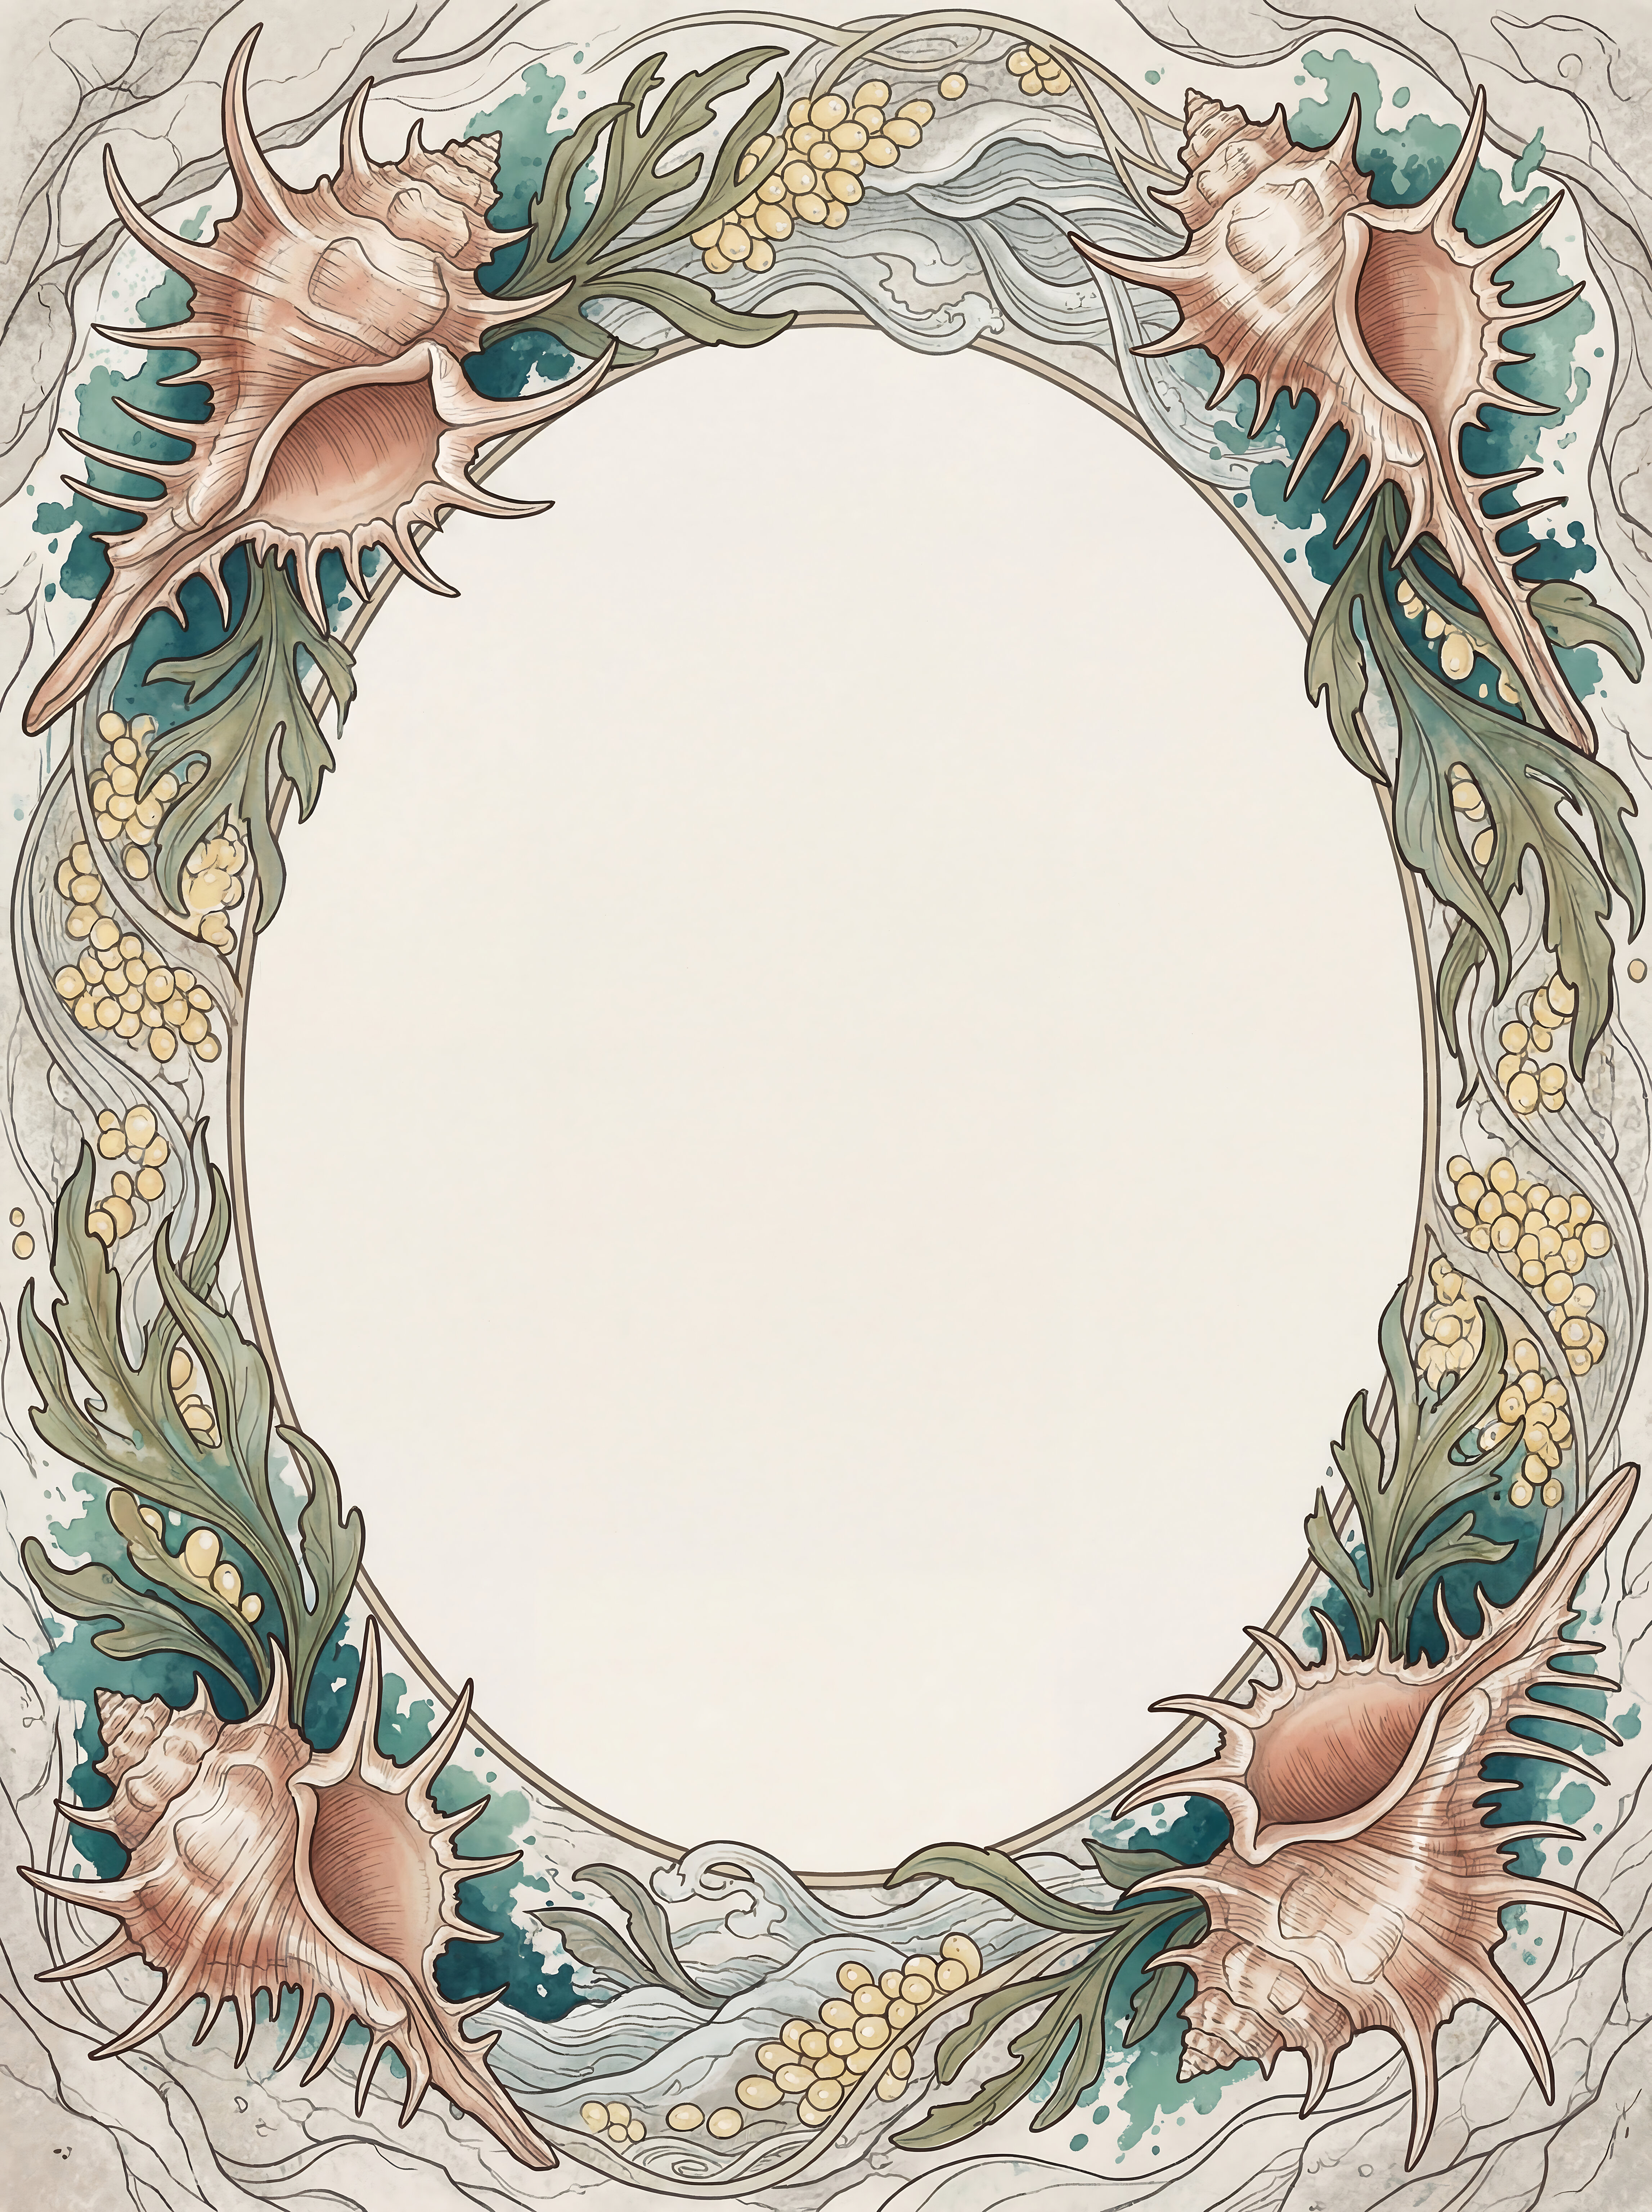
\includegraphics[width=\paperwidth,height=\paperheight]{murex-1.jpg}}
\fancypagestyle{plain}{%
\fancyhf{} % clear all header and footer fields
\fancyfoot[C]{\bfseries\scriptsize\thepage} % except the center
\renewcommand{\headrulewidth}{0pt}
\renewcommand{\footrulewidth}{0pt}
}
\pagestyle{plain}
\begin{titlepage}
    \centering                     % Center everything on the page

    % -------------------------------------------------
    % Title rules
    % -------------------------------------------------
    \rule{\textwidth}{1.6pt}\\[-\baselineskip]\vskip2pt
    \rule{\textwidth}{0.4pt}\\[1\baselineskip]

    % -------------------------------------------------
    % Title
    % -------------------------------------------------
    {\scshape\Large Libellum de Restitutione Purpurarum}\\[0.2\baselineskip]

    % -------------------------------------------------
    % Bottom title rules
    % -------------------------------------------------
    \rule{\textwidth}{0.4pt}\\[-\baselineskip]\vskip3.2pt
    \rule{\textwidth}{1.6pt}\\[1\baselineskip]

    % -------------------------------------------------
    % Subtitle (long Latin sentence)
    % -------------------------------------------------
    {\scshape Tertio editum, emendatum, et auctum \\\large Paschalis Amatius}

    {\scshape Sabinianensis\\Jurisconsultus\\D. D. D.}

    % -------------------------------------------------
    % Date / defense statement / author line
    % -------------------------------------------------


    % -------------------------------------------------
    % Place / publisher info (pushed to bottom)
    % -------------------------------------------------
    \vfill

    \begin{figure}[H]
    \centering
    \includegraphics[width=0.65\textwidth,keepaspectratio]{cover.png}
    \end{figure}

    \vfill

    {\scshape Cæsenæ, 1784\\\small Typis Gregorii Blasinii\\Præsidibus annuentibus}
 
    % -------------------------------------------------
    % Edition / license line
    % -------------------------------------------------
    {\scshape Solar Anamnesis Edition}\\[0.2\baselineskip]
    {\scshape\small CC0 1.0 Universale}
\end{titlepage}
\setlength{\parskip}{1mm plus1mm minus1mm}
\clearpage
\tableofcontents
\clearpage
\footnotesize
\section*{}
\begin{center}
\bfseries
Amplissime

Ravennatium Senator.
\end{center}
\paragraph{}
Quod post duas de flumine Rubicone a me editas dissertationes tertiam, quod post tres Italicae Bibliographiae libros, reliquos annuos adhuc desiderari permittam, cum huiusce rei caussae multae fuerint, quas referre sit longum, suffecerit spondere, me non ita longo tempore primum opus completurum, et secundum profecto maius, et toti Italicae Litteraturae apprime necessarium opus, cum juxta publicum vulgatum programma empturientium idoneus numerus fuerit contractus, breviori etiam tempore Typis Mantuanis Josephi Sbaralii prosecuturum. Non enim mea edita Collectio omnium Latinorum Poetarum, Fragmentorum, Carminum, sive ex Ethnicis, sive ex Christianis, sive ex marmoribus, sive ex membranis collectorum, quae omnes superiores Collectiones et copia et raritate carminum longissime superat, non alter meus libellus de transitu Annibalis per Apenninum, et de Castro Mutilo antiquorum Gallorum, quid plurimas Italiae antiquitates declarat, amplificationem ullam novam hactenus desiderare videntur. Contra materiae amoenitas et gravitas, Lucensis editionis paucitas, Romanae in maiori opere Musaei Kircheriani submersio, publicum non expletum desiderium, ut hanc tertiam praesentis mei de restitutione purpurarum Libelli editionem novis curis auctam nunc praeverterem, monuerunt; et deinde non minus Familiae tuae generositas, quam Mentis et Animi tui virtus, ut tibi, amplissime Ravennatium Senator, editionem ipsam nuncuparem, adduxerunt.

Nec iam hae, quas memoravimus, nuncupationis caussae minus verae. Quoad primam enim, satis mihi constat, duas nobilissimas Elephantutiorum Familias, Bononiensem alteram, quam doctus Senator Johannes Elephantutius hoc tempore exornat, Ravennatem alteram, quam hoc tempore tu exornas, gentiles et agnatas ab iisdem Maioribus ortum duxisse, tuam vero pluribus ab hinc seculis Bononia seditionibus extorrem Ravennae consedisse, ibique Romanorum Pontificum, Caroli 5. Romanorum Imperatoris, Augusti 3. Sarmatarum Regis, et Venetae Reipublicae gravissimis judiciis fuisse cohonestatam, inter Patricias Romanas, Bononienses, Ferrarienses, Firmanas, et Atrienses Familias fuisse conscriptam, illustribus cognationibus, Praesulibus, Episcopis, Cardinalibus, togatis Praetoribus, armatis Ducibus, Hierosolymorum et Divi Stephani Equitibus, Divo etiam Seraphino ex Presbyterorum ordine, et Divo Marco ex Fratrum Observantium familia fuisse illustratam, ut Caietanum Elephantutium praeclarissimum S. R. E. Cardinalem patruum tuum nuper lugentibus adhuc bonis vita functum, et Josephum et Ferdinandum fratres tuos, alterum Caroli 3. Hispaniae Regis Equitem stipatorem, alterum Romanum Praesulem, jam Camerini, jam Firmi, modo Centumcellarum Praetorem, quorum alteri Militia, alteri Roma maiores honores spondet, ingrato silentio praeteream.

Quid vero, quae secunda nuncupationis caussa, de animi tui, de mentis tuae magnitudine dicam? Tu juvenculus ad Ravennatem Rempublicam ultro accessisti, maximos magistratus ilicet inivisti, publicas pecunias, quae peribant, restituisti, Ravennatis agri culturam auxisti, novas ad portum vias aperuisti, nova ad ipsum portum aedificia extulisti, commercium, navigationem adiuvisti, Divi Alberti Conventum mutua voluntate Reipublicae Ravennati contribuisti, publicas et privatas maximas lites conciliasti, Legatus de maximis rebus missus ad Urbem gravissima illa tua et patriarum et civilium rerum cognitione Civitatis jura rata fecisti, Legatus item ad E. D. Cardinalem Boncompagnium Bononiae Legatum, de Rheni aliorumque fluminum mutatione, rem satis per se implicitam et ancipitem composuisti.

Nec vero negotiis tuis otium tuum vilius judicandum. Cum enim tu Celsiani praecepti memor, quod modo in urbe, modo in agro, sæpius in agro vitam degendam jubet, in villam tuam Gualdum idemtidem secedis, quae Caesenam inter et Ariminum sita, Viam Aemiliam adiacens, saluberrimo aere praedita, hinc Gallicam hanc planitiem, qua circumdatur, despectat, hinc amoenissimos, qui longe impendent, Apennini colles suspectat, tu ipse Agricolturam et Architectonicen bene doctus, vel cultius fertilissimum latifundium tuum instituis, vel maximam urbanam et rusticam villam a fundamentis iterum exstruis et disponis, vel in tua, quam rusticam vocas, quam philosophicam ego voco, Bibliotheca te abscondens, omnium artium, scientiarum omnium cognitione animum tuum informas, ita ut ego, qui Gualdum duobus vix millibus passuum Sabiniano distans, dum facultas datur, saepius te conventurus concedam, tecum totos dies vel legens, vel colloquens ita delecter, ut a patriarum et domesticarum rerum curis abductus, tunc tantum mihi beatam vitam vivere videar.

Quae cum ita sint, quis a me bene factum non judicet, si tibi, Vir nobilissime, et artium sollertissime, hunc tertio editum, emendatum, et auctum Libellum inscripserim, qui nobilissimam antiquarum purpurarum artem curet restituendam? Perlege igitur, et, quae tua est virtus, judica. Et si nobilitatem artis admiraberis, si restitutionis facilitatem etiam ut spero animadvertes, tum te precor quaesoque, ut quemadmodum auctorem jampridem, ita libens volens jam nunc Libellum ipsum in tuam fidem recipias.

\bigskip

Dat. Sabiniano Kalendis Januariis anni Christiani 1784.
\clearpage
\section{De duplici tincturae genere apud antiquos, purpureo, et herbaceo.}
\paragraph{}
Praefari breviter operae pretium est, plurima nova, de quibus altum in libris nostrorum hominum silentium, plurima etiam nova omnibus libris nostrorum hominum adversantia, in hoc libello esse invenienda: nos vero neminem impugnaturos, caussam tantum nostram dicturos, lectores doctos judicaturos. Quod igitur faustum, felixque sit, initium rei facimus.

Duplex omnino tincturae genus apud antiquos homines viguit: alterum conchis marinis, alterum herbis paratum: illud purpureum, hoc herbaceum nuncupatum: colores ex illo profecti, purpurei: colores ex hoc profecti, herbacei appellati. Plinius Hist. natur. lib. 8. cap. 48. \emph{Lanarum nigrae nullum colorem bibunt. De reliquarum infectu suis locis dicemus, in conchyliis marinis, aut herbarum natura.} D. Cyprianus de disciplina, et habitu virginis. \emph{Neque enim Deus... herbarum succis, et conchyliis tingere, et colorare lanas docuit.} Utrumque genus plurimos colores edidit. Colores purpurei fuerunt novem simplices, et quinque mixti. Novem colores purpurei simplices erant, niger, lividus, violaceus, rubidus, caeruleus saturatior, caeruleus dilutior, flavus, rubicundus, candidus. Quinque colores purpurei mixti erant rubidus violaceus, rubidus caeruleus saturatior, rubidus caeruleus dilutior, rubidus flavus, rubidus rubicundus. Colores herbacei plurimi etiam fuerunt. Nos de purpureis plurimum, quod opus est nostrum, de herbaceis minimum loquemur.

\section{De Colore simplici purpureo nigro.} 
\paragraph{}
Color primus purpureus simplex erat niger. Aristot. Hist. animal. lib. 5. c. 15.: Εισι δε των πορφυρων γενη πολλα... και αι μεν εν τοις κολποις μεγαλαι, και τραχειαι, και το ανθος αυτων αι μεν πλεισται μελαν εχουσαι... Ετι δε εν μεν τοις βορειοις μελαιναι... ως επι επι το πλειστον. \emph{Purpurarum sunt genera plura. Pelagiae magnae scabraeque sunt, et florem habent pleraeque nigrum... Immo in plagis ad septemtrionem vergentibus purpurae plerumque sunt nigrae.} Vitruvius Architect. lib. 7. cap. 13. \emph{Incipiam nunc de ostro dicere, quod et carissimam, et excellentissimam habet, praeter hos colores, aspectus suavitatem. Id autem excipitur ex conchylio marino, quo purpura inficitur, cujus non minores sunt, quam ceterarum naturae rerum, considerantibus admirationes, quod habet non in omnibus locis, quibus nascitur, unius generis colorem, sed solis cursu naturaliter temperatur. Itaque quod legitur Ponto et Gallia, quod hae regiones sunt proximae ad septentrionem, est atrum.} Plutarchus Catonem in ejus vita inducit purpura hac nigra fere semper obsitum. Επει πορφυραν εωρα την κατακορως ερυθραν, και οξειαν αγαπωμενην, αυτος εφορει την μελαιναν. \emph{Cum Cato vidisset purpuram vivide rubram, acutam, et amabilem, ipse nigram purpuram induit.} D. Gregorius Nyssenus in Oratione S. Theodori ait Romanos Imperatores, ut se etiam Pontifices maximos ostentarent, hujusmodi obsoleta purpura indui solitos. Tom. 2. Oper. pag. 1015. Εγω και τους βασιλεας τουτους ελεω, οτι αυταρκες εν ανθρωποις αξιωμα το κρατος της βασιλειας εχοντες, την του αρχιερεως εαυτοις προσηγοριαν ανεθεσαν, και την πενθηρη και σκοτεινην πορφυραν εκειθεν αμπισχονται, κατα μιμησιν των κακοδαιμονων αρχιερεων, αξιωματι φαιδρω, σκυθρωπον περιφεροντες ενδυμα. \emph{Me etiam Imperatorum horum miseret, quod satis magnam inter homines dignitatem regium imperium obtinentes, Pontificis appellationem sibi sumpserunt, et lugubrem obscuramque purpuram iccirco induuntur ad imitationem infelicium Pontificum, in dignitate splendida triste circumgestantes indumentum.} Cicero quoque hujusce nigrae, aut fuscae purpurae meminit in Oratione pro P. Sextio. \emph{Vestitus asper nostra hac purpura plebeia, ac pene fusca.} Meminit etiam Columella Rei rusticae lib. 2. cap. 45. \emph{Sunt complura lactucae genera... earum quae fusci, ac veluti purpurei coloris.}

\section{De Colore simplici purpureo livido.}
\paragraph{}
Color secundus purpureus simplex erat lividus, nimirum niger caeruleo mixtus. Meminit Vitruvius citato loco. \emph{Progredientibus inter septentrionem, et occidentem invenitur (conchylium) lividum.} Martialis lib. 8. epig. 28. \emph{Te nec Amyclaeo decuit livere veneno.} Statius lib. 1. Silvarum:
\begin{quotation}\bfseries\scriptsize
\hspace*{10mm}\emph{Purpura saepe}

\emph{Oebalis, et Tyrii moderator livet aheni.} Horatius lib. 2. Ode 5.

\hspace*{10mm}\emph{Jam tibi lividos}

\emph{Distinguit autumnus racemos}

\emph{Purpureo varius colore.}
\end{quotation}
\paragraph{}
Purpura quaedam apud antiquos in laude erat, quae Ferrugo ab ipsis appellaretur. Virgilius Aeneidos lib. 9.:
\begin{quotation}\bfseries\scriptsize
\emph{Pictus acu chlamydem, et Ferrugine clarus Ibera.}
\end{quotation}
Et lib. 2. ejusdem Aeneidos:
\begin{quotation}\bfseries\scriptsize
\emph{Ipse peregrina Ferrugine clarus et Ostro.}
\end{quotation}
\paragraph{}
Jam vero haec purpura Ferrugo ipsa haec erat livida purpura. Servius ad memoratum Virgilii versum lib. 9. Aeneidos. \emph{Ferrugo coloris genus est, qui vicinus est purpurae subnigrae.} Idem Servius ad lib. 1. Georgices: \emph{Ferrugine texit. Ferrugo est purpura nigrior Hispana.} Nec audiendi qui colorem ferrugineum, vel purpurae Ferruginis, subrubrum fuisse autumant, nimirum rubiginosum, aut rubiginis ferri similem. Jam enim audivimus Servium eum subnigrum, sive lividum, non vero subrubrum vocantem. Plinius deinde lib. 29. cap. 6. lacertas describit \emph{virides ferrugineis maculis distinctas}, et lacertarum maculae nobis liquidissime non subrubrae, aut rubiginosae, sed lividae apparent. Plautus in Milite Act. 4. Scen. 4. ferrugineum colorem maris colori comparat. \emph{Palliolum habeas ferrugineum, nam is color thalassicus est.} Nosque ipsi mare lividum conspicimus, cum remis, aut ventis agitatur, ut etiam mox clarius enarrabimus. Observandum denique voces ferrugineus, et Ferrugo a voce Ferrum liquido descendere, non vero a voce Rubigo, a qua tantum vox rubiginosus proficisci videtur. Ferrum autem, si tersum et politum sit, quodque optime nos Itali \emph{ferro imbrunito} appellare consuevimus, colorem lividum, sive nigrum caeruleo mixtum clarissime ostendit. Immo Nonius ipse hanc coloris ferruginei a ferro originem fere probat. \emph{Ferrugineum colorem ferri similem esse volunt. Vere autem ferrugineus color caeruleus est.} Et licet ille ibidem ferrugineum caeruleum malit, imprudens tamen rem nostram confirmat. Ferrum enim ipsum tersum caeruleum est, quamvis atrore mixtum, et proinde est lividum, uti demonstravimus.

Color quoque Venetus antiquorum non jam caeruleus, uti plerique sentiunt, sed ferrugineus, et lividus, uti haec purpura Ferrugo, sive niger caeruleo mixtus erat. Cresconius Corippus lib. 1. Panegyrici in laudem Justini 2. colorem Venetum non tantum assimilat vel Ferrugini, cujus colorem lividum vidimus, vel Ostro, cujus colorem subnigrum mox videbimus, sed etiam colori uvarum nigrarum, et olivarum, cum maturae fuerint.
\begin{quotation}\bfseries\scriptsize
\emph{Autumni Venetus ferrugine dives et ostro}

\emph{Maturas uvas, maturas signat olivas.}
\end{quotation}
\paragraph{}
Quis vero non viderit uvas nigras, et olivas maturescentes omnino lividas, et proinde Veneti coloris? Columella ipse lividas esse maturas olivas affirmavit lib. 14. cap. 47. \emph{Oliva livorem contrahit.} Et lividas uvas maturas Horatius lib. 2. Ode 5.
\begin{quotation}\bfseries\scriptsize
\hspace*{10mm}\emph{Jam tibi lividos}

\emph{Distinguit autumnus racemos}

\emph{Purpureo varius colore.}
\end{quotation}
\paragraph{}
Corippus ipse eodem loco quatuor celebres partium Circi colores, nimirum album, rubrum, venetum, prasinum, quatuor anni temporibus ita assimilat:
\begin{quotation}\bfseries\scriptsize
\emph{Aurigas totidem, totidem posuere colores.}

\emph{Nam viridis vernis campus ceu concolor herbis,}

\emph{Pinguis oliva comis, luxu nemus omne virescit.}

\emph{Russeus aestati rubra sic veste refulgens,}

\emph{Ut nonnulla rubent ardenti poma colore.}

\emph{Aequiparans candore nives, hiemisque pruinas}

\emph{Albicolor viridi socio conjungitur una.}

\emph{Autumni Venetus ferrugine dives et ostro}

\emph{Maturas uvas, maturas signat olivas.}
\end{quotation}
\paragraph{}
Ita vero eos ipsos colores quatuor eisdem anni temporibus assimilat Cassiodorus lib. 3. \emph{Colores autem in vicem temporum quadrifaria divisione funduntur. Prasinus virenti verno, Venetus nubilae hiemi, Roseus aestati flammeae, Albus pruinoso autumno dicatus est.} Si igitur Venetum colorem Corippus autumno, Cassiodorus hiemi assimilat, quis etiam non videat horum duorum anni temporum pluvios, et turbidos dies, vere lividos, non vero caeruleos posse vocitari? Mare etiam remis aut undis agitatum est lividum, et proinde ad significandum hunc colorem purpureum lividum, quem omnino ostendit, vocitatum fuisse purpureum ipsum mare ab omni Graeca, et Latina antiquitate non dubitemus. Cicero Academic. lib. 3. \emph{Mare illud, quod Favonio nascente purpureum videtur.} Idem Cicero in Academicis apud Nonium in Verbo \emph{purpurascit}. \emph{Quid mare, nonne caeruleum, aut ejus unda, cum est pulsa remis, purpurascit?} Plinius lib. 9. cap. 36. \emph{Sed unde conchyliis pretia? Quid virus grave in fuco, color austerus in glauco, et irascenti similis mari?} Furius Antias apud Gellium Noct. Attic. lib. 18. cap. 2.:
\begin{quotation}\bfseries\scriptsize
\emph{Spiritus Eurorum virides cum purpurat undas.}

\hspace*{10mm}Propertius lib. 2. eleg. 18.

\emph{purpureis agitatam fluctibus Hellen.}

\hspace*{10mm}Virgilius Georgices lib. 4.:

\emph{Eridanus, quo non alius per pinguia culta}

\emph{In mare purpureum violentior incidit amnis.}
\end{quotation}
\paragraph{}
Et Servius ad illos versus: \emph{Purpureum autem nigrum ex altitudine accipimus. Nam Padus non in rubrum mare, sed juxta Ravennam in Adriaticum cadit. Et purpureum Graecum est epithetum. Mare rubrum etiam dixit Homerus. Unde apparet Victorinum hoc loco errasse, qui purpureum mare rubrum esse dixit, quod est juxta Indiam.} Et re quidem vera Homerus praeter ceteros Graecos pluries dixit, εις υδασι πορφυρεοισιν, \emph{in purpureis aquis}, εις αλα πορφυροεσσαν, \emph{in purpureum mare}, nempe in lividum mare, uti contra Virgilius aperte lividas Lethis aquas vocavit Aeneidos lib. 6.:
\begin{quotation}\bfseries\scriptsize
\emph{remis vada livida verrunt.}
\end{quotation}
\paragraph{}
Et uti Catullus Carm. 18. lividissimas Benaci aquas nuncupavit:
\begin{quotation}\bfseries\scriptsize
\emph{Verum totius ut lacus, putidaeque paludis}

\emph{Lividissima, maximeque est profunda vorago.}
\end{quotation}
\section{De Colore simplici purpureo violaceo.}
\paragraph{}
Color tertius purpureus simplex erat violaceus. Vitruvius eodem citato loco. \emph{Quod autem (conchylium) legitur ad aequinoctialem orientem et occidentem, invenitur violaceo colore.} Plinius lib. 21. cap. 8. \emph{Alium (colorem) in amethysto, qui in viola, et ipsum purpureum, quemque janthinum appellamus.} Et sane adeo similis erat tertius iste simplex purpureus color violae martiae colori, ut ab eo ipso flore, qui ιον Graece vocatur, nomen coloris violacei et janthini traxerit. Immo ipsa viola martia procul dubio purpurea vocata fuit ad hunc purpureum violaceum colorem significandum, quem numeris omnibus absolutum praeseferebat. Cornelius Nepos apud Plinium lib. 9. cap. 39. \emph{Me, inquit, juvene violacea purpura vigebat.} Horatius lib. 2. epist. 1.
\begin{quotation}\bfseries\scriptsize
\emph{Lana Tarentino violas imitata veneno.}

\hspace*{10mm}Venantius Fortunatus Poem. 7. lib. 7.

\emph{Aureus ordo crocis, violis hinc blatteus exit.}

\hspace*{10mm}Idem Fortunatus Poem. 8. lib. 7.

\emph{Purpura per violas, aurea forma crocus.}
\end{quotation}
\paragraph{}
Plinius idem lib. 21. cap. 6.: \emph{Violis honos proximus. Earum plura genera; purpureae, luteae, albae. Ex iis vero, quae sponte apricis et macris locis proveniunt, purpureae... Graeco nomme a ceteris discernuntur, appellatae ιον, ut ab his janthina vestis.} Martialis lib. 2. epigr. 39.
\begin{quotation}\bfseries\scriptsize
\emph{Coccina famosae donas et janthina moechae.}
\end{quotation}
\paragraph{}
Similis erat etiam tertius iste simplex purpureus color amethysto, quae gemma est violaceo colore affatim perfusa. Plinius non tantum citato loco, sed etiam lib. 37. cap. 19. \emph{Alius ex hoc ordo purpureus dabitur, et ab illis descendentibus. Principatum amethysti Indicae tenent... Caussam nominis afferunt, quod usque ad vini colorem accedens, prius quam eum degustet, in violam desinat, fulgorque quidam in illa sit purpurae, non ex toto igneus, sed in vini colorem deficiens. Perlucent autem omnes violaceo colore. Indicae absolutum felicis purpurae colorem habent, ad hancque tingentium officinae dirigunt vota.} Hinc ipse color purpureus violaceus vocabatur etiam amethystinus, amethystinaeque vocabantur illae vestes, quae hoc colore violaceo tingerentur. Juvenalis Sat. 7.
\begin{quotation}\bfseries\scriptsize
\hspace*{10mm}\emph{Purpura spondet}

\emph{Caussidicum, spondent amethystina.}

\hspace*{10mm}Martialis lib. 1. epigr. 97.

\emph{Amethystinasque mulierum vocat vestes.}

\hspace*{10mm}Idem Martialis lib. 2. epigr. 57.

\emph{Amethystinatus media qui secat septa.}

\hspace*{10mm}Venantius Fortunatus lib. 7. poem. 3.

\emph{Ailigat et nitidos amethystina vitta capillos.}
\end{quotation}
\paragraph{}
Hinc etiam ad hunc purpureum violaceum colorem significandum procul dubio vocatae fuerunt purpureae hae ipsae amethysti a Plinio in laudato loco. \emph{Alius ex hoc ordo purpureus dabitur... Principatum amethysti indicae tenent.} Et ab Ovidio de arte amandi lib. 3.
\begin{quotation}\bfseries\scriptsize
\emph{Hic Paphias myrtus, hic purpureas amethystos.}
\end{quotation}
\paragraph{}
Flos etiam Amelli colore suo absolute referebat hunc ipsum violaceum purpureum colorem, et proinde ipse flos, eo quod violaceus, purpureus dictus est a Columella, et aperte purpureus violaceus a Virgilio. Columella lib. 9. \emph{Amelli radix, cujus est frutex luteus, purpureus flos.} Virgilius Georgices lib. 4.
\begin{quotation}\bfseries\scriptsize
\emph{Est etiam flos in pratis, cui nomen Amello}

\emph{Fecere agricolae, facilis quaerentibus herba.}

\emph{Aureus ipse, sed in foliis, quae plurima circum}

\emph{Funduntur, violae sublucet purpura nigrae.}
\end{quotation}
\paragraph{}
\section{De colore simplici purpureo rubido Tyrio.}
\paragraph{}
Quartus purpureus color simplex rubidus erat, nimirum ruber nigritie multa mixtus. Plinius lib. 21. cap. 8. \emph{Alium (colorem) in purpuris Tyriis, dibaphisque et Laconicis.} Jam vero hae purpurae Tyriae et Laconicae rubidae erant, et rubidis floribus papaverum concolores. Manilius Astronomicon lib. 5. 
\begin{quotation}\bfseries\scriptsize
\emph{Liliaque, et Tyrias imitata papavera luces.}
\end{quotation}
\paragraph{}
Nec non etiam rubido sanguini concreto, rubidisque rosis, quas \emph{Damascenas} vocant, similes erant. Plinius ipse lib. 9. cap. 36. \emph{Purpurae florem illum tingendis expetitum vestibus in mediis habent faucibus. Liquoris hic minimi est in candida vena, unde pretiosus ille bibitur nigrantis rosae color sublucens... Color sanguinis concreti nigricans aspectu, idemque suspectu refulgens... Rorem eum excipientes Tyrii. Praecipuus hic Asiae, in Meninge Africae, et Gaetulo littore Oceani, in Laconica Europae.} Hinc Cassiodorus lib. 1. epist. 2. emphatice hunc colorem purpureum rubidum, obscuritatem rubentem, et nigredinem sanguineam vocat. \emph{Color nimio lepore vernans, obscuritas rubens, nigredo sanguinea regnantem discernit, dominum conspicuum facit, et praestat humano generi, ne de conspectu principis possit errari.}

Rubida etiam sunt mora matura, et ideo ad purpureum hunc colorem rubidum significandum, quem clare promunt, purpurea mora ipsa vocata fuerunt ab Ovidio Metamorphoseon lib. 4., quo loco enarrat sanguinem Pyrami et Thisbes rubido suo colore mora ipsa infecisse.
\begin{quotation}\bfseries\scriptsize
\emph{Arborei foetus aspergine caedis in atram}

\emph{Vertuntur faciem, madefactaque sanguine radix}

\emph{Purpureo tingit pendentia mora colore...}

\emph{Signa tene caedis, pullosque et luctibus aptos}

\emph{Semper habe foetus gemini monumenta cruoris...}

\emph{Vota tamen tetigere Deos, tetigere parentes,}

\emph{Nam color in pomo est, ubi permaturuit, ater.}
\end{quotation}
\paragraph{}
Uvas quoque nigras non aliter quam uvas purpureas vocavere antiqui homines, hac ipsa significatione rubidi coloris, quem apprime ostentant. Virgilius lib. 2. Georgicon. \emph{Uvae purpureae.} Horatius Ode 2. Epodon.
\begin{quotation}\bfseries\scriptsize
\emph{Certantem et uvam purpurae.}

\hspace*{10mm}Ovidius lib. 4. Metamorphoseon.

\emph{Purpura fulgorem pictis accommodat uvis.}

\hspace*{10mm}Et lib. 8.

\emph{Et de purpureis collectae vitibus uvae.}

\hspace*{10mm}Et denique lib. 13.

\emph{Sunt auro similes longis in vitibus uvae.}

\emph{Sunt et purpurae. Tibi et has servamus et illas.}

\hspace*{10mm}Plinius lib. 14. cap. 2.
\end{quotation}
\paragraph{}
\emph{Hic (vites) purpureo lucent colore, illic fulgent roseo, nitentque viridi.} Capitolinus in Maximini vita. \emph{Posita ab eodem vitis intra annum ingentes uvas purpureas attulit.} Vopiscus in Taciti vita. \emph{Vitis quae uvas Ammineas albas ferebat, eo anno, quo ille imperium meruit, purpurascere plurima purpura coepit.}

Hinc lapis etiam quidam Lapis purpureus, sive Porphyrites, sive Porphyra (unde Italicum verbum \emph{Porfido}) ab antiquis hominibus appellabatur; eo quod rubidum hunc colorem purpureum aliquot tantum maculis albis interlitum praeseferret, uti quisque novit.

Eminebat Constantinopoli ampla domus hoc uno lapide constans, et ideo Purpura, sive πορφυρα vocata, quam ita eleganter describit Anna Comnena Alexiados lib. 7. Η δε πορφυρα οικημα τι εστι κατα τα αναητορα εξ αυτης της βασεως μεχρι της οροφου κινησεως δια τετραγωνου συμπληρουμενων σχηματος, εκειθεν δε εις πυραμιδα αποτελευτων. αφορων μεν ως προς ταλατταν προς τον λιμενα, ουπερ οι πετρινοι βοες, και οι λεοντες. δια μαρμαρων δε το τε εδαφος κατεστρωτο, και οι τοιχοι περιστελλοντο, ου των τυχοντων, ουδε των αλλων οποσοι εμποριστοτεροι των τιμιωτερων λιθων εισιν, αλλ' εξ ων απο ρωμης οι ανεκαθεν βασιλεις επεσυραντο. Εστι δε ουτος ο λιθος ολως ειπειν πορφυρους δι' ολου, και οιον στιγματα τινα ψαμμυειδη λευκα αυτω περιτρεχουσιν. Εκ τουτωνι των λιθων πορφυραν το οικημα οι ανεκαθεν ωνοματαν. \emph{Est autem} Purpura \emph{aedificium quoddam prope imperiale Palatium ab ipsa basi usque ad tecti suggrundia quadrata constructum forma, hinc in pyramidem desinens. Prospectum habet mare versus in eum portum, in quo lapidea visuntur boum et leonum simulacra. Marmore solum constructum est, et parietes tecti. Marmor porro istud non jam est ex vulgatis, neque ex excellentioribus, quotquot sunt magis parabilia, sed ex illis, quae ab urbe Roma primi Imperatores transtulerunt. Est is lapis purpureus totus, et tantum punctula alba arenae specie eum percurrunt. Ex hisce lapidibus Purpuram hoc aedificium antiqui vocaverunt.}

Inserviebat autem haec porphyretica domus Augustarum puerperiis, et hinc Porphyrogenetae appellabantur Graecorum Imperatorum filii, non qui post comparatam a Patre imperii purpuram, sed qui in hac domo, quae Purpura, sive lapis purpureus vocabatur, nati essent. Eadem Anna Comnena Olympiados lib. 6. Ο δε βασιλευς... την βασιλιδα κατα το αωρισμενον καλαι ταις τικτουσαις των βασιλιδων οικημα επι ταις ωδισιν ευρηκως, (πορφυραν δε τουτο οι ανεκαθεν ονομαζουσιν, εξ ου και το των πορφυρογεννητων ονομα εις την οικουμενην διεδραμεν). \emph{Ceterum Imperator... Augustam suam conjugem in dicata antiquitus puerperiis Augustarum aede in partus doloribus cum reperisset, (Purpuram autem ab antiquis temporibus hanc aedem vocant, unde Porphyrogenetarum nomen orbe toto manavit.)} Hic tamen, quamvis abs re fuerit, animadvertere liceat, Annam Comnenam relato loco adfirmantem, primos Constantinopolitanos Imperatores porphyreticos hosce lapides usque ab urbe Roma transtulisse, et proinde judicare fas sit, ipsum Constantinum Magnum hanc domum instruxisse lapidibus illis porphyreticis, quibus jam Elagabalus plateas Romani Palatii stravisset, quosque lapides Lampridius ipse Constantino Maevus inde paucis ante annis eductos, quam ille historiam suam scriberet, adfirmat. Ita ille in Elagabali vita. \emph{Stravit (Elagabalus) et saxis Lacedaemoniis ac Porphyreticis plateas in Palatio, quas Antoninianas vocavit, quae saxa usque ad nostram memoriam manserunt, sed nuper eruta sunt.}

\section{De Colore simplici purpureo caeruleo saturatiore, sive hyacinthino.}
\paragraph{}
Quintus color purpureus simplex erat caeruleus austerior, et violaceo mixtus. Julius Pollux Onomastici lib. 1. cap. 4. το δε αιμα, επειδαν πυρι ομιληση, χειθαι τε, και εξανθει. και το μεν ξανθιζεται, το δε κυαναυγες γιγνεται, το δε αλλο εις αλλην χροαν τρεπεται. \emph{Sanguis (conchyliorum) cum igni efferbuerit, diffunditur, et efflorescit. Et alius quidem fit flavus, alius caeruleus austerus, aliusque in alium vertitur colorem.} Plinius lib. 21. cap. 13. \emph{Tertius est, qui proprie conchylii intelligitur, multis modis. Unus in Heliotropio, et in aliquo ex his plerumque saturatior.} Enimvero Heliotropium antiquorum florem hujusmodi habebat caeruleum saturatiorem. Plinius ipse lib. 21. cap. 21. \emph{Heliotropii caeruleum florem.} Hunc ipsum etiam Heliotropii florem uti caeruleum luridum, et violaceo mixtum ita describit Ovidius Metamorphoseon lib. 4. puellam Clytiam in hunc ipsum florem conversam enarrans.
\begin{quotation}\bfseries\scriptsize
\hspace*{10mm}\emph{partemque coloris}

\emph{Luridus exsangues pallor convertit in herbas.}

\emph{Est in parte rubor, violaeque simillimus ora}

\emph{Flos tegit. Illa suum, quamvis radice tenetur,}

\emph{Vertitur ad solem, mutataque servat amorem.}
\end{quotation}
\paragraph{}
Quidquid igitur dicant nostri Botanici homines, Heliotropium antiquorum flos ille non erat, quem nos Itali \emph{Girasole} vocitamus, quique non caeruleo, sed flavo flore coruscat. Quodnam igitur Heliotropium antiquorum? Certe Heliotropium, quod Graeci nominabant. Latini Intubum agreste appellabant. Vegetius Veterinariae lib. 3. cap. 62. \emph{Heliotropii unciam, quod intubum agreste vocamus.} Neque id ullo modo dubitandum, Intubum enim sive agreste, sive sativum oculis nostris testibus, et ad solem vertitur, et caeruleum florem habet saturatiorem, sive violaceo mixtum, uti diximus.

Hac vero purpura caerulea fulgebat praecipue Regum Persarum diadema. Curtius enim eodem libro 6. modo caeruleum, modo purpureum diadema ipsum vocat. Ita ille de Dario loquens: \emph{Cidarim Persae regium capitis voc abant insigne: hoc caerulea fascia albo distincta circuibat.} Et mox de Magno Alexandro loquens: \emph{Itaque purpureum diadema distinctum albo, quale Darius habuerat, capiti circumdedit.}

Eadem caerulea purpura concolori caeruleo caelo inficiebantur etiam fimbriae Hebraeorum juxta divinum praeceptum Num. cap. 20. Maimonides apud Bochartum Hierozoicon part. 2. lib. 5. cap. 9. \emph{Cum fimbriarum thecheleth (seu purpuram) infecturi sunt... sanguinem} του \emph{chilzon (conchae purpurae) afferunt... et lanam in eum immergunt, donec fiat caelo concolor.}

Hyacinthus, Vaccinium, Iris, Gladiolus, unus erat apud antiquos idemque flos, licet ipsi nostri Botanici homines eos distinguere satius ducant. Primo enim Virgilius Graecum Hyacinthum Theocriti in suum Latinum Vaccinium perspicue vertit. Ita Theocritus Idyll. 10.:
\begin{quotation}\bfseries\scriptsize
και το ιον μελαν εστι, και αγραπτα Υακινθος.

\hspace*{10mm}Ita Virgilius eclog. 10.:

\emph{Et nigrae violae sunt, et vaccinia nigra.}
\end{quotation}
\paragraph{}
Clarius etiam Philargyrius antiquus interpres ad lib. 4. vers. 183. Aeneidos: \emph{Qui Graece Hyacinthus, Latine Vaccinium dicitur.} Quoad reliqua vero duo nomina Iridis, et Gladioli clare Columella lib. 9. cap. 4. \emph{Caelestis nominis Hyacinthus.} Nimirum Iridis caelestis nomine donatus. Clarius etiam Palladius Rei rust. lib. 1. cap. 37.: \emph{Hyacinthus, qui Iris, vel Gladiolus dicitur.} Hic vero flos quadruplici nomine ornatus apud antiquos, ille ipse flos erat, quem nos Itali \emph{Giglio paonazzo} appellamus; quique moenia Sabinianensium, qua ad meridiem vergunt, florido vere sponte nascens caerulea purpura exornat, proximoque oppidi vico nomen etiam \emph{di contrada del Giglio} impertitur. Rem ita esse ut probetur, audiamus sane descriptionem illius floris, quam nobis antiqui reliquerunt. Ita igitur eum describit Servius ad eclog. 3. vers. 106. Virgilii: \emph{Hyacinthus ubique nascitur, flos, qui natus est primo de Hyacinthi sanguine, postea de Aiacis, sicut etiam Ovidius docet. Est autem quasi lilium rubrum designans primam Hyacinthi litteram.} Ita vero Ovidius immutatum referens in hunc ipsum florem puellum Hyacinthum Metamorphoseon lib. 10.:
\begin{quotation}\bfseries\scriptsize
\emph{Ecce cruor, qui fusus humi signaverat herbas,}

\emph{Desinit esse cruor, Tyrioque nitentior ostro}

\emph{Flos oritur, formamque capit quam lilia, si non}

\emph{Purpureus color his, argenteus esset in illis.}

\emph{Ipse suos gemitus foliis inscripsit, et ai ai}

\emph{Flos habet inscriptum.}
\end{quotation}
\paragraph{}
Jam vero eadem magnitudo, et eadem figura liliorum alborum, color caeruleus saturatior, sive violaceo mixtus, qui maximus est Iridis caelestis color, nonnullae lineae florem transcurrentes, et fabulosas litteras \emph{ai ai} referentes, folia ipsa tam floris, quam plantae longa, et acuta, et proinde simillima gladio, et simillima Υ primae litterae Graeci vocabuli Υακινθος, hae omnes eaedem proprietates sunt, quae a Servio, et ab Ovidio antiquo flori Hyacintho tribuuntur, quaeque in hunc florem, quem \emph{Giglio paonazzo} appellamus, adamussim congruere videntur.

Jam vero hic, quem descriptimus, flos Hyacinthus colorem caeruleum saturatiorem, sive violaceo mixtum ostendit, testibus oculis nostris, testibus antiquis scriptoribus ipsis. Columella lib. 10. vers. C. eum vocat aperte caeruleum: \emph{caeruleos hyacinthos}. Virgilius vero eclog. 10. vers. 39. nigrum hyacinthum non secus ac nigras violas refert, quasi huic flori colorem caeruleum austeriorem, aut violaceo mixtum donaturus:
\begin{quotation}\bfseries\scriptsize
\emph{Et nigrae violae sunt, et vaccinia nigra.}
\end{quotation}
\paragraph{}
Hinc idem hic flos Hyacinthus ratione coloris hujus purpurei caerulei saturatioris purpureus appellatus fuit ab Ovidio laudato loco referente puellum Hyacinthum in hunc ipsum florem conversum:
\begin{quotation}\bfseries\scriptsize
\hspace*{5mm}\emph{formamque capit, quam lilia, si non}

\emph{Purpureus color his, argenteus esset in illis.}
\end{quotation}
\paragraph{}
Et ab eodem Ovidio Metamorphoseon lib. 13. Aiacem in hunc ipsum florem conversum enarrante:
\begin{quotation}\bfseries\scriptsize
\hspace*{5mm}\emph{rubefactaque sanguine tellus}

\emph{Purpureum viridi genuit de cortice florem.}

\hspace*{10mm}Ita etiam ipse Ovidius Tristium lib. 1. eleg. 1.:

\emph{Nec te purpureo velent vaccinia succo.}

\hspace*{10mm}Manilius Astronomicon lib. 5. vers. 268.

\emph{Pallentes violas, et purpureos hyacinthos.}

\hspace*{10mm}Euphorion:

πορφυρεη Υακινθε σε τουνομα φασιν αοιδοι

\emph{Purpureae hyacinthe, te nomine vocant Poetae.}
\end{quotation}
\paragraph{}
Lucianus in amoribus: Υακινθοις το καλον ανθουσιν ομοια πορφυροντες. \emph{Cincinni perinde ac pulchre florentes hyacinthi purpurascentes.}

Immo hanc ipsam purpuram caeruleam saturatiorem antiqui homines ab hoc eodem flore Hyacinthinam appellare consueverunt. Persius Sat. 1.:
\begin{quotation}\bfseries\scriptsize
\emph{Heic aliquis, cui circum humeros hyacinthina laena est.}
\end{quotation}
\paragraph{}
Venantius Fortunatus lib. 4. Vitæ B. Martini:
\begin{quotation}\bfseries\scriptsize
\emph{ubi lana hyacinthina currit.}
\end{quotation}
\paragraph{}
Tertullianus in libro habitus mulierum: \emph{Parietes Tyriis, et Hyacinthinis... pro pictura abutuntur.} Vopiscus in Bonosi Vita: \emph{Tunicas palliolatas hyacinthinas subsericas.} Lex Theodosii a Justiniano relata in Codicem suum ad titulum: \emph{Quae res vendi possunt. Fucandae, atque distrahendae purpurae vel in serico, vel in lana, quae blatta, vel oxyblatta, atque hyacinthina dicitur.}

\section{De Colore simplici purpureo caeruleo dilutiore, sive molochino.}
\paragraph{}
Sextus color purpureus simplex erat caeruleus dilutior, sive caeruleus rubicundo mixtus. Plinius laudato pluries loco: \emph{Alius (color) in malva ad purpuram inclinans.} Quis vero nesciat flores notissimos ubique nascentis malvae hocce colore caeruleo dilutiore, sive mixto cum rubro, laetissime perfusos? Nec alius erat profecto color molochinus antiquorum, quam iste purpureus caeruleus dilutior, ita dictus a malva, quae μολοχη Graece dicitur. Nonius: \emph{Molochinum a Graeco color est flori similis malvae.} Immo Nonius ipse referre non dubitat hunc Caecilii versum molochinas vestes nuncupantem:
\begin{quotation}\bfseries\scriptsize
\emph{Carbasina, molochina, ampelina.}
\end{quotation}
\paragraph{}
Et etiam Plauti versum molochinarios hujusmodi purpurae caeruleae dilutioris infectores vocantem:
\begin{quotation}\bfseries\scriptsize
\emph{Astant molochinarii, petunt fullones.}
\end{quotation}
\paragraph{}
Non me latet verbum μαλακος solere verti \emph{mollis}. Animadvertere tamen hic liceat, hanc ipsam vocem μαλακος ab ipsa malva, quae Graece etiam μαλαχη dicitur, proficisci. Deinde quoque observandum mollissimas fuisse purpuras omnes, uti cap. 30. enunciabimus. Fieri igitur facile possit, ut vox μαλακος a μαλαχη, quae eadem malva est, proficiscatur, et non jam mollem, sed purpureum, immo hunc ipsum purpureum colorem caeruleum dilutiorem, qui floris malvae similis sit, significare videatur. Muratorius pag. 939. n. 6. sui Thesauri Inscriptionum hanc epigraphen nobis refert: P. AVCTIVS P. F. LYSANDER VESTIARIVS TENVARIVS MOLOCHINARIVS. Hinc idem Muratorius subdit: \emph{Vestiarius Tenuarius is dicebatur, qui vestes tenuiores conficiebat. Molochinarius, qui ejusmodi vestes molochini coloris parabat. Audi Nonium etc. Caecilium etc. Plautum etc. At malva Graecis μαλαχη malache appellata est: quod nomen aliis Graecis est μολοχη moloche. Proinde non uno errore labitur Isidorus lib. 19. cap. 22. Originum, dum scribit: Molochinia vestis, quae malvarum stamine conficitur.}

\section{De Colore simplici purpureo flavo.}
\paragraph{}
Septimus color purpureus simplex erat flavus. Julius Pollux relato loco: το μεν ξανθιζεται. \emph{Sanguis conchyliorum aliquando flavescit...} Plinius vero loco eodem colori violae serotinae, seu autumnalis comparat. \emph{Alius (color) in viola serotina conchyliorum vegetissima.} Quae autumnalis, aut serotina viola flava erat, cum Plinius ipse calthae concolorem faciat lib. 21. cap. 6.: \emph{Calathiana (viola) munus autumni, caeterae veris. Proxima ei caltha est concolori amplitudine.} Indubium autem est, calthae florem esse flavo colore nitescentem, tum testibus oculis, tum teste Italo nomine \emph{di Fiorrancio}, quo caltham indigitamus, testibus denique ipsis antiquis scriptoribus. Virgilius eclog. 2.:
\begin{quotation}\bfseries\scriptsize
\emph{Mollia luteola pingit vaccinia caltha.}

\hspace*{10mm}Columella lib. 10. vers. 97.

\emph{Candida leucoia, et flaventia lumina calthae.}
\end{quotation}
\paragraph{}
Immo ipse Plinius lib. 21. cap. 11. assimilat violam ipsam serotinam flammae colori, quem flavum videmus, et a quo ipsa viola nomine Graeco phlox, nimirum flammea etiam nuncupabatur. \emph{Florum prima ver nunciantium viola alba. Postea quae appellatur purpurea. Proxime flammea, quae et phlox vocatur.} Columella eodem lib. 10. vers. 101. hanc violam auro ipsi, quod flavum est, assimilat:
\begin{quotation}\bfseries\scriptsize
\hspace*{5mm}\emph{quae frondens purpurat auro,}

\emph{Ponatur viola.}
\end{quotation}
\paragraph{}
\section{De Colore simplici purpureo rubicundo.}
\paragraph{}
Octavus color purpureus simplex erat rubicundus. Aristoteles Histor. anim. lib. 5. cap. 15.: ενιαι δ' ερυθρον μικρον... αι δ' εν τοις αιγιαλοις, και περι τας ακτας το μεν μεγεθος γινονται μικραι. το δε ανθος ερυθρον εχουσιν... εν δε τοις νοτιοις ερυθραι, ως επι το πλειστον. \emph{Purpurae quaedam florem habent aliquantulum rubrum. Quae vero in sinibus degunt, aut circa littora, magnitudine parvae sunt, habent autem florem rubrum... In plagis vero ad meridiem vergentibus purpurae plerumque rubrae sunt.} Vitruvius eodem lib. 7. cap. 13. \emph{Quod vero (conchylium) meridianis excipitur regionibus, rubra procreatur potestate, et ideo hoc rubrum Rhodo etiam insula creatur, ceterisque hujusmodi regionibus, quae proximae sunt Solis cursui.} Haec vero purpura rubicunda a Graecis purpura οξυς, sive acuta vocabatur, eo quod rubicundus color ceteris naturae coloribus sit vere acutior, et vividior. Plutarchum jam audivimus in Catonis vita vocantem πορφυραν κατακορως ερυθραν, και οξειαν. \emph{Purpuram valde rubram, et acutam.} Legem quoque Theodosii audivimus, a qua nominatur purpura, quae blatta, vel oxyblatta dicitur. Addatur denique Cedrenus in Vita Tiberii 2.: των μερων φορουντων στολας σωληνωτας απο βλαττιου οξεος. \emph{Factionibus Circi ferentibus stolas purpura acuta virgatas.}

Meminit 1. C. Ulpianus purpurae cujusdam, quam Buccinum vocat. Ita ille in L. Si cui lana D. De Legatis 3. \emph{Appellatione purpurae... Buccinum et Hyacinthinum continebitur.} Haec autem Buccini purpura haec ipsa erat rubicunda purpura, cum concha illa, cui Buccino nomen erat, et quae nomen huic ipsi purpurae praestabat, colorem coccineum praeberet, qui profecto color erat rubicundus, uti cap. 16. probabimus. Plinius relato lib. 9. cap. 38.: \emph{Buccinum... dat austeritatem illam, nitoremque, qui quaeritur, Cocci.} Hic tamen observandum, ceteros quidem omnes purpureos colores fuisse immortales, ut cap. 29. palam fiet, hunc vero rubicundum colorem Buccini vocatum, celer. rime evanescere, et extingui consuevisse. Plinius eodem loco. \emph{Rubeus color nigrante deterior. Buccinum per se damnatur, quoniam fucum remittit.} Locus etiam Quintiliani huc referendus. Ait itaque hic egregius Rhetor lib. 12. cap. 10. Rhetorices, orationem floridis argutiis plenam placere, cum primum audias, uti vestis infecta coloribus non purpureis placet: eandem deinde orationem minus placere, si cum altera matura oratione comparetur, uti etiam minus placet vestis coloribus non purpureis infecta, si cum purpurea tantum lacerna comparetur: (lacernae enim tunc temporis omnes purpureae erant, uti plura etiam unius Martialis carmina undequaque hoc libro relata satis probant) ipsam denique orationem ad severum examen revocatam, et frigiditate argutiarum detecta, eo inenarrabili modo deformem visum iri, uti Buccini purpuram, cum haec illum suum colorem rubicundum, quem parvo tempore ementita fuerit, tandem omnino dimiserit. \emph{Sed evanescunt haec, atque emoriuntur comparatione meliorum, ut lana tincta fuco citra purpuram placet: at si contuleris etiam lacernae, conspectu melioris obruatur, ut Ovidius ait. Si vero judicium his corruptis acrius adhibeas, ut Buccini purpura, jam illud quod fefellerat, exuat mentitum colorem, et quadam vix enarrabili foeditate pallescat.}

\section{De Colore simplici purpureo candido.}
\paragraph{}
Nonus color purpureus simplex erat candidus. Plinius lib. 37. cap. 19. \emph{albicante purpurae dejectu.} Codinus in cap. 2. Officiorum Ecclesiae et Aulae Constantinopolitanae nuncupat λευκον βλατιον, \emph{purpuram candidam}. Plutarchus in Alexandri Magni vita hunc Regem affirmat in Perside magnam purpurae rubicundae, et candidae vim reperisse: Οπου φασι και πορφυρας Ερμιονικης ευρεθηναι ταλαντα πεντακισχιλια, συγκειμενης μεν εξ ετων δεκα δεοντων διακοσιων, προσφατον και το ανθος ετι και νεαρον φυλαττουσης. αιτιον δε τουτου φασιν ειναι, το την βαφην δια μελιτος γινεσθαι των αλουργων, δι ελαιου δε λευκου, των λευκων. και γαρ τουτων τον ισον χρονον εχοντων την λαμπροτητα καθαραν, και στιλβουσαν ορασθαι.

\emph{Ubi ajunt reperta talenta quinquaginta millia purpurae Hermionices a ducentis fere annis repositae, et servantis adhuc recentem florem, et colorem suum. Cujus rei caussam esse dicunt, quod purpurarum rubicundarum tinctura melle paretur, tinctura autem purpurarum candidarum oleo albo. In his enim purpuris, cum tempus memorato aequale habuerint, purus, et lucidus splendor apparet.}

Albinovanus bis reperitur vocasse purpuream nivem, quae candida sit, in Elegia in obitum Maecenatis.
\begin{quotation}\bfseries\scriptsize
\emph{Purpurea sub nive terra latet.}

\emph{Brachia purpurea candidiora nive.}
\end{quotation}
\paragraph{}
Horatius lib. 4. ode 1. vocavit purpureos etiam candidos cycnos.
\begin{quotation}\bfseries\scriptsize
\emph{Purpureis ales oloribus.}
\end{quotation}
\paragraph{}
Denique Ovidius, et Catullus purpuream nuncuparunt ipsam candidissimam lucem. Ita Ovidius:
\begin{quotation}\bfseries\scriptsize
\emph{Laetaque purpurea luce refulsit humus.}

\hspace*{10mm}Catullus Epithal. Pelei, et Thetidis.

\emph{Purpureaque procul nantes a luce refulgent.}
\end{quotation}
\paragraph{}
Satagunt commentatores, et Grammatici, ut haec translata verba esse nobis fidem faciant. Nos credimus haec propria, et candorem nivis, lucis, olorum candido colori hujus purpurae ab hisce scriptoribus propriissime comparatum. Si qua enim purpura candida non fuisset, nae infelicissime scriptores isti candidam nivem, candidam lucem, candidos olores cum purpureis coloribus, quorum nullus candidus esset, comparassent.

\section{De Coloribus simplicibus purpureis generatim.}
\paragraph{}
Novem igitur fuere purpurei colores marinis conchis producti, quos simplices vocamus. Primus erat niger. Secundus erat lividus, ferrugineus, venetus, aut niger caeruleo mixtus, similisque colori livido ferri tersi, olivarum maturarum, uvarum nigrarum, et maris a ventis, remisque agitati. Tertius erat violaceus, similis violaceo colori violae martiae, amethysti, et amelli. Quartus erat rubidus, similis colori rubido papaverum, sanguinis concreti, rosarum nigrarum, quas Damascenas vocant, mororum, uvarum rubidarum, et lapidis purpurei, sive Porphyritis. Quintus caeruleus saturatior, sive caeruleus violaceo mixtus erat, similisque colori caeruleo saturo sereni caeli, heliotropii, hyacinthi. Sextus erat caeruleus dilutior, sive caeruleus rubro mixtus, similisque colori caeruleo dilutiori florum malvae. Septimus erat flavus, similis colori flavo violae serotinae, calthae, flammae, et auri. Octavus erat rubicundus. Nonus denique erat candidus, similis candori nivis, et lucis, et cycnorum.

Nulla profecto res nos fallere potuit in definiendis, metandisque hisce novem purpureis coloribus simplicibus. Nos antiquos Scriptores audivimus affirmantes, eosdem novem purpureos colores similes omnino fuisse relatorum naturalium corporum coloribus. Immo asseverat Plinius antiquos purpurarios artifices, cum purpuras conderent, eorundem naturalium corporum colores suis hisce factitiis purpureis coloribus quam vividissime imitari, et exprimere, et fere cum natura ipse certare consuevisse. Ita ille lib. 37. cap. 19. \emph{Indicae amethysti absolutum felicis purpurae colorem habent, ad hancque tingentium officinae dirigunt vota.} Et lib. 21. cap. 8. \emph{Luxuria vestibus quoque provocavit eos flores, qui colore commendantur.} Hinc purpureorum colorum, et florum, corporumque, quae diximus, concolori similitudine descripta, haec addit. \emph{Paria nunc componuntur, et natura, atque luxuria depugnant.} Colores igitur florum, et corporum, quos retulimus, archetypa sunt, et novem simplices factitii purpurei colores, quos descripsimus, imagines erant. Si imagines periere, supersunt adhuc ea archetypa, quae de veritate purpureorum novem colorum simplicium, de quibus hactenus verba sunt facta, nihil nobis dubitandum esse spondeant.

\section{De divisione Colorum simplicium purpureorum.}
\paragraph{}
Saepiuscule nominat eodem loco Plinius colores purpurae, et colores conchylii, uti duos colores omnino distinctos, et diversos. Ita ille lib. 6. cap. 29. de Tyro loquens. \emph{Nunc omnis ejus (Tyri) nobilitas conchylio, atque purpura constat.} Et lib. 29. cap. 35. \emph{Sed quota haec portio est reputantibus purpuras, conchylia, margaritas?} Ita pariter lib. 8. cap. 48. \emph{Vidimus jam et viventium vellera purpura, cocco, conchylio infecta.} Et demum lib. 37. cap. 9. \emph{Gallia herbis Tyrium, atque conchylium tingit.} Ita etiam Svetonius in vita Caligulae cap. 17. \emph{Pueris, ac feminis fascias purpurae, ac conchylii distribuit.} Sed hujusmodi distinctionem declarat ipse Plinius lib. 21. cap. 8. asserens primum purpuram Tyriam, aut Laconicam rubidam, et purpuram violaceam, aut amethystinam vocari proprie, et peculiariter purpuras, aut purpureos colores. \emph{Hos colores animadverto tres esse principales. Unum... in purpuris Tyriis, dibaphisque, et Laconicis. Alium in amethysto, qui in viola, et ipsum purpureum, quemque janthinum appellamus.} Asserit deinde Plinius eodem loco, purpuram caeruleam saturam similem heliotropio, purpuram caeruleam dilutam similem flori malvae, et purpuram flavam similem violae serotinae, proprie et peculiariter vocari consuevisse conchylia, aut conchylii colores: \emph{tertius est, qui proprie conchylii intelligitur, multis modis. Unus in heliotropio, et in aliquo ex his plerumque saturatior. Alius in malva ad purpuram inclinans. Alius in viola serotina conchyliorum vegetissima.} Immo Plinius ipse hujusce distinctionis duas adfert caussas, nimirum infectionis discrimen, et discrimen coloris. Illi duo purpurae colores abundantioribus succis, hi tres conchylii colores parcioribus tingebantur. Rursus illi duo purpurae colores ob ipsam medicaminum copiam austeriores, hi tres conchylii colores ob medicaminum ipsorum parcitatem dilutiores, et laetiores erant. Ita ipse Plinius lib. 9. cap. 38. \emph{Concharum ad purpuras et conchylia}, (en redit constans colorum purpurae, et colorum conchylii distinctio) \emph{eadem quidem est materia, sed distat temperamento.} Ita deinde Plinius eodem loco describit illarum duarum purpurarum rubidae, et violaceae tincturam. \emph{Buccinum... Pelagio admodum alligatur... ita fit amethysti color eximius ille. At Tyrius Pelagio primum satiatur... mox permutatur in Buccino.} Demum ita eodem loco enarrat horum trium conchyliorum tincturam, nimirum caerulei saturi, caerulei diluti, et flavi. \emph{In conchyliata veste cetera eadem sine buccino... dimidia et medicamina adduntur. Sic gignitur laudatus ille pallor saturitate fraudata, tantoque dilutior, quanto magis vellera esuriunt.} Erant igitur colores rubidi, et violacei austeriores colores, majori succorum copia compositi, et fere plenae, et absolutae purpurae. Erant tres colores caerulei saturi, caerulei diluti, et flavi, minori succorum copia producti, et fere semiplenae, aut imperfectae purpurae. Factum igitur, ut antiqui ad hoc non minimum discrimen demonstrandum, illos duos primos proprie vocarent colores purpureos, istos vero tres postremos proprie colores conchyliatos nominarent, licet utrique, utpote iisdem marinis conchis educti, colores purpurei generatim nominarentur, et essent. Sed de hoc ipso colorum purpurae, et colorum conchylii discrimine plenius in cap. 25. agetur.

An autem purpuris, sive conchyliis reliquos quatuor purpureos simplices colores, nigros, lividos, rubicundos, candidos antiqui contribuerint, omnino latet, cum eos Plinius ne quidem commemoret. Veri autem simile est praeteriisse Plinium quatuor illos purpureos colores, quod fere essent rariores, et obsoleti; nigri quidem, et lividi, eo quod inamoeni; rubicundi, eo quod facile evanescentes; candidi, quod proprii Persarum, et Indorum, et in Romano Imperio inusitati, et fere nulli essent, ut cap. 20. videbimus. Cum tamen Plinius unos colores caeruleos saturos, caeruleos dilutos, et flavos conchylii colores nuncupet, eosque unos dilutiores, et parcioribus succis conditos affirmet, pro certo est habendum, quatuor reliquos memoratos colores jam purpureos, non conchyliatos ab antiquis vocitari, et haberi consuevisse. Cum igitur antiquos scriptores invenerimus reminiscentes colores conchyliatos, nae intelligamus unos colores caeruleos, aut flavos, non vero ceteros purpureos colores, qui hac peculiari significatione nullo modo continerentur. Ita locus Plauti intelligendus Pseudoli. act. 1. scen. 2. 
\begin{quotation}\bfseries\scriptsize
\emph{Neque Alexandrina belluata conchyliata tapetia.}
\end{quotation}
\paragraph{}
Ita etiam Cicero Philip. 2. \emph{Conchyliatis Gn. Pompeii peristromatis servorum in cellis lectos stratos videres.} Seneca ep. 62. \emph{Demetrium virorum optimum mecum circumfero, et relictis conchyliatis cum illo seminudo loquor, illum admiror.} Juvenalis Sat. 8.
\begin{quotation}\bfseries\scriptsize
\hspace*{5mm}\emph{stahat acervus}

\emph{Nummorum, Spartana chlamys, Conchylia Coa.}

\hspace*{10mm}Idem Juvenalis Sat. 3.

\emph{Horum ego non fugiam conchylia?}
\end{quotation}
\paragraph{}
Svetonius in Caesaris vita. \emph{Usum conchyliatae vestis ademit.} Ita denique ceteri omnes scriptores intelligendi, qui colorum conchylii meminerint, quosque brevitatis gratia praeterimus.

\section{De coloribus purpureis mixtis.}
\paragraph{}
Quinque porro erant colores mixti purpurei, uti cap. 1. diximus.

Primus autem color mixtus purpureus ex colore amethystino violaceo, et ex Tyrio rubido componebatur, et iccirco color Tyrianthinus, aut Tyriamethystinus vocabatur. Plinius ipse lib. 9. cap. 40. 41.: \emph{Sed alia sunt e fine initia, juvatque ludere impendio et lusus geminare miscendo iterum et ipsa adulteria naturae... Non est satis abstulisse gemmae nomen amethystum: rursus absolutus inebriatur Tyrio, ut sit ex utroque nomen improbum, (Tyriamethystinus) simulque luxuria duplex.} Vopiscus in Carini vita: \emph{Inscriptum est adhuc in choraulae pallio Tyrianthino... Messalae nomen et uxoris.} Martialis lib. 1. epig. 54.
\begin{quotation}\bfseries\scriptsize
\emph{Sic interpositus vitio contaminat uncto}

\emph{Urbica Lingonicus Tyrianthina bardocucullus.}
\end{quotation}
\paragraph{}
Observavimus superiore capite colores caeruleos saturos, caeruleos dilutos, et flavos, proprie colores conchyliatos, aut conchylii vocitatos fuisse. Secundus igitur mixtus color ex Tyrio rubido, et caeruleo saturatiore componebatur, quemadmodum tertius ex Tyrio rubido, et caeruleo dilutiore, et quartus tandem ex ipso Tyrio rubido, et flavo componebatur. Plinius eodem loco: \emph{Et cum confecere conchylia, transire melius in Tyrium putant.} Si enim cum Tyrio rubido miscebant antiqui colores conchylii, qui erant caeruleus satur, caeruleus dilutus, et flavus, hos tres colores mixtos descendere necesse fuit, nimirum rubidum caeruleo saturo mixtum, rubidum caeruleo diluto mixtum, rubidum denique flavo mixtum, uti diximus.

Quintus denique color purpureus mixtus ex ipso Tyrio rubido, et ex colore coccineo, qui rubicundus est, uti cap. 16. videbimus, componebatur. Plinius eodem loco: \emph{Quin et terrena miscere, coccoque tinctum Tyrio tingere, ut fieret Hysginum.} Color igitur Hysginus, de quo plurimi scriptores meminere, quos consulto praeterimus, color erat ex rubido, et rubicundo mixtus, et fere inter utrumque medius. Sed iterum de hisce mixtis coloribus purpureis cap. 25. loquemur.

Si igitur observatum est, colores purpureos fuisse novem simplices, et quinque mixtos, jam clarissime patet, purpuram non fuisse peculiarem colorem aliquem, quae vulgaris omnium nostrorum hominum est opinio, sed potius tincturae genus, quo fere omnes iidem colores producerentur, qui herbis aut vegetabilibus produci consuevissent.

\section{De Ostro.}
\paragraph{}
Non imus inficias Ostrum fuisse plerumque nomen cuilibet purpureo colori significando commune, nomenque ipsum ab οστρεον, quod concham marinam significat, esse profectum, ut ait ipse Vitruvius lib. 7. cap. 13.: \emph{Quod ex concharum marinarum testis eximitur, ideo ostrum est vocitatum.} Non id tamen semper accidit: immo plerumque ostrum uni colori purpureo rubido significando proprie assignatum observavimus.

Considerandum enim est primo nomen ostri unis purpuris Sidoniis, Tyriis, et Punicis tantum adtributum fuisse, quae procul dubio rubidae erant, uti cap. 5. vidimus. Pauca haec testimonia veterum pluribus omissis suffecerint.
\begin{quotation}\bfseries\scriptsize
\hspace*{10mm}Propertius lib. 3. eleg. 13.:

\emph{Et Tyros ostrinos praebet Cadmea colores.}

\hspace*{10mm}Idem Propertius lib. 4. eleg. 3.:

\emph{Nam mihi, quo Poenis tibi purpura fulgeat ostris.}

\hspace*{10mm}Ovidius Heroidum epist. 12.:

\emph{Rideat, et Tyrio jaceat sublimis in ostro.}

\hspace*{10mm}Idem Ovidius Metamorphoseon lib. 10.:

\emph{Desinit esse cruor, Tyrioque nitentior ostro}

\emph{Flos oritur.}

\hspace*{10mm}Statius Sylvarum lib. 5.:

\emph{Hic te Sidonio velatam molliter ostro.}

\hspace*{10mm}Silius Italicus Punicorum lib. 8.

\emph{Et princeps Tyrio vestem praetexuit ostro.}
\end{quotation}
\paragraph{}
Alcimus Avitus nuncupat quoque ostrum Sidonium, et ostrum ipsum Sidonium a purpura distinguit, quam sorsan purpuram violaceam intelligit. Ita ille Poematum lib. 6.:
\begin{quotation}\bfseries\scriptsize
\emph{Nec te Sidonium bis cocti muricis ostrum}

\emph{Induit, aut rutilo permulcens purpura fuco.}
\end{quotation}
\paragraph{}
Considerandum est secundo, Corippum in Panegyrico 1. in laudem Justini 2. enarrare, in quadam veste ejusdem Justini homines pugnantes auro, sanguinem vulnerum ostro pictum:
\begin{quotation}\bfseries\scriptsize
\emph{Effigies auro, sanguis depingitur ostro.}
\end{quotation}
\paragraph{}
Cum autem sanguis concretus sit rubidus, rubidum quoque esse debebat ostrum, quod ostrum ipsum sanguinem significare, et exprimere deberet.

Tertio loco hic Virgilii versus ex lib. 2. Aeneidos est observandus:
\begin{quotation}\bfseries\scriptsize
\emph{Ipse peregrina ferrugine dives, et ostro.}
\end{quotation}
\paragraph{}
Minus propriam enim et Virgilio indignam Virgilius ipse partitionem hic nobis obtrusisset, si nomen proprium peculiaris purpurae, quae Ferrugo vocabatur, ut cap. 3. vidimus, cum nomine Ostro conjunxisset, quod appellativum, ut ajunt Grammatici, et commune coloribus omnibus purpureis designandis fuisset. Sed neutiquam putandum divinum Virgilium ita pueriliter errasse, potiusque dicamus Virgilium eundem, quemadmodum ferruginis nomine peculiarem purpuram lividam intellexerit, ita nomine ostri peculiarem aliquam purpuram intellexisse, et praesertim rubidam Tyriam. Et re quidem vera eodem laudato loco Corippus ipse Ferruginem, et Ostrum conjungit, sed sui ipsius, et ejusdem Virgilii sententiam ostendens, alteram purpuram lividis olivis, alteram vero purpuram rubidis uvis aequiparat, et proinde clare Ferruginem purpuram lividam, Ostrum purpuram Tyriam rubidam esse declarat:
\begin{quotation}\bfseries\scriptsize
\emph{Autumni Venetus ferrugine dives, et ostro}

\emph{Maturas uvas, maturas signat olivas.}
\end{quotation}
\paragraph{}
Nonius denique in notis ad Turpilium Poetam in Veliterna Comoedia ostrinum colorem subrubeum, sive rubidum clarissime nuncupat. \emph{Ostrinum ab Ostro colore, qui est subrubeus.}

\section{De coloribus herbaceis.}
\paragraph{}
Quemadmodum vero antiqui homines plurimos colores conchis marinis producebant, ita quoque plurimos cudebant colores herbis, et vegetabilibus. Primum itaque eosdem fere omnes colores, quos e conchis marinis eduxisse hactenus vidimus, herbis, et vegetabilibus fingebant. Plinius lib. 22. cap. 2. \emph{Jam vero infici vestes scimus admirabili fuco... transalpina Gallia herbis Tyrium, atque conchylium tingit, omnesque alios colores, nec quaerit in profundis murices... ut inveniat, per quod facilius matrona adultero placeat, corruptor insidietur nuptae. Stans et sicco carpit, quod frugi mundos exculpat.} Idem Plinius lib. 21. cap. 26. \emph{Hyacinthus in Gallia eximie provenit. Hoc ibi pro cocco hysginum tingitur.} Plurimas vero rationes herbis simulandi purpureos omnes colores, sive simplices, sive mixtos, quos diximus, diligentissime tradunt Plinius ipse in sua naturali Historia, Vitruvius in Architectura, Julius Pollux in suo Onomastico, aliique antiqui Scriptores, qui consulendi.

Ut vero hi colores memoratis purpureis similes, qui herbis conficerentur, discrimine aliquo notarentur ab iisdem coloribus, qui vere conchis marinis compositi fuissent, hi purpurae maritimae, illi purpurae tantum colores dici consuevere. Julius Pollux Onomastici lib. 7. cap. 13. Ο δε κανδυς ο μεν βασιλειος αλιπορφυρος, ο δε των αλλων πορφυρους. \emph{Vestis autem regia ex purpura maritima erat, aliorum vero e purpura tantum.} Multa loca, quae expresse mentionem faciunt πορφυρας θαλαττιας, \emph{purpurae marinae}, habes apud Bochartium \emph{Hierozoicon} Par. 2. lib. 5. cap. 14.

Verum post hos omnes colores purpureos herbis, ut ita dicam, recusos, plurimos alios etiam colores herbis effingere solebant antiqui homines. Nobis autem, utpote de coloribus tantum purpureis tractaturis, uti diximus, suffecerit horum colorum floridissimus catalogus, quem nobis praebet Ovidius de Arte amandi lib. 3.
\begin{quotation}\bfseries\scriptsize
\emph{Quid de veste loquar? Nec vos, segmenta, requiro,}

\hspace*{5mm}\emph{Nec quae bis Tyrio murice, lana, rubes.}

\emph{Cum tot prodierint pretio leviore colores,}

\hspace*{5mm}\emph{Quis furor est census corpore ferre suo?}

\emph{Aeris ecce color, tunc cum sine nubibus aer,}

\hspace*{5mm}\emph{Nec tepidus pluvias concitat auster aquas.}

\emph{Ecce tibi similis, qui quondam Phryxon, et Hellen}

\hspace*{5mm}\emph{Diceris Inois eripuisse dolis.}

\emph{Hic undas imitatur, habet quoque nomen ab undis.}

\hspace*{5mm}\emph{Crediderim Nymphas hac ego veste tegi.}

\emph{Ille crocum simulat, croceo velatur amictu,}

\hspace*{5mm}\emph{Roscida luciferos cum Dea jungit equos.}

\emph{Hic Paphias myrtus, hic purpureas amethystos}

\hspace*{5mm}\emph{Albentesve rosas, Threiciamque gruem.}

\emph{Nec glandes, Amarylli, tuae, nec amygdala desunt,}

\hspace*{5mm}\emph{Et sua velleribus nomina cera dedit.}

\emph{Quot nova terra parit flores, cum vere tepenti}

\hspace*{5mm}\emph{Vitis agit gemmas, pigraque cedit hiems,}

\emph{Lana tot, aut plures succos bibit...}
\end{quotation}
\paragraph{}
De numero autem colorum plurimorum, qui (praeter colores purpureis similes,) herbis conficerentur, deque eorundem conficiendorum ratione, iidem scriptores, quos supra retulimus, consulendi.

\section{De Colore coccineo.}
\paragraph{}
Celeberrimus vero colorum, qui herbis conficerentur, procul dubio erat coccineus. Color is e cocco, unde nomen accipiebat, producebatur. Coccus juxta antiquorum sententiam nihil aliud erat, quam granum quoddam, quod magna copia nascebatur in Africa, in Galatia, in Lusitania. Plinius lib. 9. cap. 41. \emph{Coccum Galatiae rubens granum, ut dicemus in terrestribus, aut circa Emeritam Lusitaniae in maxima laude est.} Et in lib. 22. cap. 2. \emph{Jam vero infici vestes scimus admirabili fuco. Atque ut sileamus Galatiae, Africae, Lusitaniae granis Coccum Imperatoriis dicatum paludamentis... tingi.} Theophrastus in Hist. Plant. lib. 3. cap. 16., Dioscorides lib. 3. cap. 16. Pausanias lib. 4. cap. 18. lib. 10., et Strabo lib. 10. plurimum de Cocco loquuntur, ad quos missos facimus lectores. Juxta vero recentiores observationes Coccus granum non est, sed Galla ex ilice quadam prognascens, aut potius quidam vermiculus, qui, ubi interierit, distenditur, grandescit, fitque Galla ovis refertissima, e quibus ovis plurimi rubicundi vermiculi progignuntur, qui ab Arabibus \emph{Chermes} vocantur, et e quorum rubicundo sanguine color iste coccineus formari solet. Percrebrescit, et viget adhuc hujusce coccinei coloris artificium, isque ipse est color, quem nos Itali, \emph{colore di scarlatto, di grana, chermisi, overmiglio}, a genitoribus vermibus nomine profecto appellamus, uti est notissimum. Immo color ipse, qui nupera nostra \emph{Coccinilia} effingitur, ut nomen ipsum declarat, vel ratione vermium, vel ratione \emph{coloris}, cocci quoque similis est. Nemo vero nescit, hunc colorem, quem adhuc oculis videmus, vividissime rubicundum esse. Id dixere tamen etiam antiqui scriptores. Plinius lib. 21. cap. 8. eum rosarum colori comparat, qui quoque vividissime est rubicundus. \emph{Unum (colorem) in cocco, qui in rosis micat: gratius nihil traditur aspectu.} Theophrastus, et Hesychius eumdem cocci colorem phoeniceum vocant, hoc est rubicundum: phoeniceus enim color est rubicundus, uti capite sequenti est demonstrandum. Ita ille lib. 3. cap. 16. κοκκον φοινικουν: \emph{Coccum Phoeniceum}. Ita hic. κοκκος φοινικουν χρωμα. \emph{Coccus color phoeniceus}. Ita etiam Horatius Sat. 6.
\begin{quotation}\bfseries\scriptsize
\hspace*{5mm}\emph{rubro ubi cocco}

\emph{Tincta super lectos canderet vestis eburnos.}

\hspace*{10mm}Venantius Fortunatus Poem. 7. lib. 7.

\emph{Aureus ordo crocis, violis hinc blatteus exit,}

\emph{Coccinus hinc rubicat, lacteus inde nivet.}

\hspace*{10mm}Sedulius Carminum lib. 4.

\hspace*{5mm}\emph{rubri vilem sub tegmine cocci}

\emph{Vestitur chlamydem.}
\end{quotation}
\paragraph{}
\section{De Colore puniceo, aut phoeniceo.}
\paragraph{}
Certe color puniceus, aut phoeniceus non erat purpureus, cum antiqui scriptores iisdem locis purpureum, et puniceum, uti duos diversos colores distinguant. Plautus Menaechmis act. 5. scen. 5.
\begin{quotation}\bfseries\scriptsize
\emph{Quin tu me interrogas, purpureum panem,}

\emph{An puniceum soleam ego esse, an luteum.}

\hspace*{10mm}Lucretius lib. 2.

\emph{Purpura, poeniceusque color clarissimu' multo.}

\hspace*{10mm}Paullinus Petrocorius in B. Martini vita lib. 3.

\emph{Dives in excelsis splendescit purpura fulcris,}

\emph{Mollia puniceo motantur serica fuco.}

\hspace*{10mm}Cresconius Corippus lib. 1. Panegyrici in laudem Justini 2.

\emph{Purpureo surae resonant fulgente cothurno,}

\emph{Cruraque puniceis induxit regia vinclis.}
\end{quotation}
\paragraph{}
Athenaeus Deipnosophistarum lib. 5. πρωτοι μεν οι τον οχλον ανειργοντες Σειληνοι, πορφυρεας χλαμυδας, οι δε φοινικιδας εμφιεσμενοι. \emph{Primi Sileni submoventes turbam purpureas chlamydes, alii vero puniceas induebantur.}

Varro autem, et Propertius non modo puniceum a purpureo distinguunt, sed etiam colorem, et coloris nomen ab Africa, et a Poenis profectum autumant. Ita Varro lib. 4. de Lingua Latina. \emph{Purpureum a purpurae maritimae colore. Poeniceum quod primum a Poenis dicitur adlatum.} Propertius lib. 4. eleg. 3.
\begin{quotation}\bfseries\scriptsize
\emph{Illi selectos certent praebere colores}

\emph{Africa puniceum, purpureumque Tyros.}
\end{quotation}
\paragraph{}
Abundat autem Africa cocco, ut affirmavit Plinius superiori Capite relatus, et proinde puniceum, aut phoeniceum colorem fuisse oportuit rubicundum, immo ipsum coccineum. Aulus Gellius lib. 2. cap. 26. Noct. Attic. \emph{Nam poeniceus, quem tu Graece φοινικα dixisti, noster est: et rutilus, et spadix phoenicei συνωνυμα, qui factus Graece noster est, et exuberantiam, splendoremque significat ruboris, quales sunt fructus palmae arboris non admodum sole incocti, unde spadicis, et phoenicei nomen est. Spadica enim Dorici vocant avulsum e palma termitem cum fructu.} Plutarchus in Pompeii, et Bruti vita vocavit: \emph{puniceam tunicam}, φοινικουν χιτωνα, tunicam illam rubicundam, quam Romani Imperatores ante tabernaculum, uti pugnae signum, proponerent, quae ipsa tunica ab eodem Plutarcho in Fabii vita χιτων κοκκινος, \emph{tunica coccinea} vocata fuit. Isidorus. \emph{Russata, quam Graeci phoeniceam vocant, nos coccinam.} Horatius Epodon ode 9.
\begin{quotation}\bfseries\scriptsize
\emph{Terra, marique victus hostis punico}

\emph{Lugubre mutavit sagum.}
\end{quotation}
\paragraph{}
Et ad eumdem locum Porphyrion. \emph{Hoc est, deposuit coccineam chlamydem Antonius, qua scilicet Imperator utebatur, et accepit lugubrem, idest nigram.}

\section{De Colore Blatteo, vel Blattae.}
\paragraph{}
Contra autem blatteus, vel blattae color coccineus non erat, cum et coccineum, et blatteum colorem eodem loco antiqui scriptores, uti duos distinctos colores, nominent. Lampridius in Elagabali vita. \emph{Paraverat igitur funes blatta, serico, et cocco intortos, quibus, si necesse esset, laqueo vitam finiret.} Venantius Fortunatus Poem. 7. lib. 7. non tantum coccineum, et blatteum colorem, uti diversos, eodem loco nuncupat, sed etiam coccineum rubicundum, et blatteum violaceum, idest purpureum declarat.
\begin{quotation}\bfseries\scriptsize
\emph{Aureus ordo crocis, violis hinc blatteus exit,}

\emph{Coccinus hinc rubicat, lacteus inde nivet.}
\end{quotation}
\paragraph{}
Immo idem Fortunatus lib. 9. Poem. 10., uti purpureum conceptis verbis colorem blatteum nuncupat.
\begin{quotation}\bfseries\scriptsize
\emph{Albent purpureis ubi lactea lilia blattis.}
\end{quotation}
\paragraph{}
Eutropius quoque blatteos, et Orosius purpureos funes retium appellat, quibus Nero piscabatur. Ita Eutropius: \emph{Nero hamis aureis, argenteisque piscabatur, qui blatteis funibus extrahebantur.} Ita Orosius. \emph{Nero retibus aureis piscabatur, quae purpureis funibus extrahebantur.} Sidonius Apollinaris Carm. 5. purpuris celeberrimam Tyrum laudat, uti blattae genitricem.
\begin{quotation}\bfseries\scriptsize
\emph{Pontus Castorea, blattam Tyrus, aera Corinthus.}
\end{quotation}
\paragraph{}
Idem Sidonius lib. 9. epist. ultim. blattiferum vocat Senatum, quem purpura, non cocco ornatum cap. 39. observabimus.
\begin{quotation}\bfseries\scriptsize
\emph{Blattifer vel quam tribuit Senatus.}
\end{quotation}
\paragraph{}
Ipse Sidonius lib. 9. epist. 13. Blattas vocat bis tinctas, nimirum clare purpuras, quae bis, uti cap. 25. confirmabimus, tingebantur.
\begin{quotation}\bfseries\scriptsize
\emph{Rutilasque ferte Blattas,}

\emph{Recoquente quas aheno}

\emph{Meliboea fucat unda,}

\emph{Opulentet ut meraco}

\emph{Bibulum colore vellus.}
\end{quotation}
\paragraph{}
Blattas bis tinctas, sive purpuras nominat etiam Alcimus Avitus Poemat. lib. 3.
\begin{quotation}\bfseries\scriptsize
\emph{Ipse cothurnatus gemmis, et fulgidus auro,}

\emph{Serica bis coctis mutabat tegmina blattis.}
\end{quotation}
\paragraph{}
Denique clarissime Blattam esse purpuram, non coccineum colorem, declarat 50. 1. lib. 40. in Codice Justinianaeo. \emph{Fucandae, atque distrahendae purpurae vel in serico, vel in lana, quae blatta, vel oxyblatta, vel hyacinthina dicitur.}

Sed quaenam origo hujusce vocis Blattae, qua posteriores Latini, Graecique purpuram nuncupabant? Graeca antiqua Glossaria auctorem adferunt quemdam \emph{Actuarium}, qui adfirmat, Blattam sibi velle os nasi, sive rostri, quo concavo ad exerendam linguam donari conchas purpuras cap. 22. enarrabimus. Ita \emph{Actuarius} ipse a Glossis relatus. Βλαττιον βυζαντιον οστουν της ρινος της πορφυρας. \emph{Blatta Byzantia os nasi purpurae.} Mattiolius, Lemerius, aliique Pharmaceutici quoddam celebre Blattion Byzantion describunt, ex quo nonnullae elapsis saeculis, uti ex cornu cervino, medicinae parabantur. Verum hoc Pharmacopolarum Blattion Byzantion nihil aliud est profecto, quam ipsum concharum, quas purpuras vocant, rostrum, uti cuilibet observare licet in Pharmacopolarum tabernis, et in tabulis ipsis incisis apud Mattiolium, aliosque hujusmodi Pharmaceuticos, et confirmat etiam Rondeletius lib. 2. cap. 15. de Testaceis. Veri igitur simile est, antiquos rostrum conchae purpurae primum, et postea concham purpuram totam nomine Blattae donasse, et deinde nomen ipsum Blattae, et purpurae a conchis blattis, et purpuris ad purpureos ipsos colores, qui ex illis effingerentur, significandos transduxisse. Immo etiam coniectura probabili assequi possumus, cur Blattam rostrum conchae purpurae Graeci nuncupaverint. Audiemus Cap. 22. conchas purpuras ceterarum concharum cortices, ut eas devorarent, solidissimo hoc suo rostro tundere, et effringere consuevisse. Vocavere igitur Graeci hoc rostrum Blattion a verbo βλαπτω, quod sibi vult laedere, et percutere, quasi rostrum reliquas conchas percutiens, et laedens significarent. Ab eadem voce βλαπτω felicius forsitan nostrum ipsum Italicum verbum \emph{battere}, quam a quovis alio longius petito, et intorto etymo promanare videtur.

\section{De discrimine Coloris coccinei, et purpureorum.}
\paragraph{}
Male coccineus color cum purpureis confundi consuevit. Omnes enim purpurei colores a coccineo, et nomine, et materia, et colore ipso longissime distabant. Et primum color coccineus, et purpureus, uti duo omnino distincti colores, nomine ipso ab antiquis scriptoribus distinguuntur. Plinius lib. 37. cap. 7. \emph{Unam, quae purpura radiet, alteram quae cocco.} Et lib. 13. cap. 48. \emph{Vidimus jam et viventium vellera purpura, cocco, conchylio infecta.} Svetonius in Neronis vita. \emph{Piscatus est reti aurato, purpura, coccoque funibus textis.} Lampridius in Diadumeni vita. \emph{Hic ubi primum indumenta coccea, et purpurea, ceteraque castrensia Imperii insignia accepit.} Martialis lib. 5. epig. 23.
\begin{quotation}\bfseries\scriptsize
\emph{Non nisi vel cocco madida, vel murice tincta}

\emph{Veste nites, et te sic dare verba putas.}

\hspace*{10mm}Et in lib. 3. epig. 2.

\emph{Et te purpura delicata velet,}

\emph{Et cocco rubeat superbus index.}
\end{quotation}
\paragraph{}
Secundo materia ipsa coccineus color, et purpurei longissime distabant. Nos cap. 25. docebimus, colores purpureos conchis marinis confectos fuisse. Vidimus vero cap. 16. coccineum colorem ex galla terrestri, quae coccus appellabatur, esse profectum.

Tertio, colore ipso differebant. Rubicundus erat color coccineus, uti cap. 16. vidimus. Colores autem purpurei in omnes alias colorum partes ibant, quam in rubicundi partes. Aderat quidem, quam supra diximus, purpura rubicunda, sed haec infrequens valde, utpote quae vigens tantum in Perside, vel India, perraro in orbis Romani regiones transduceretur, et quae rubicunda purpura in orbis Romani regionibus aliquando conficeretur ope majoris succi buccinorum, quam purpurarum, (unde etiam Buccini purpura vocabatur) ita evanida erat, et obnoxia corruptioni, ut hoc nomine damnata ab omnibus vix ac ne vix quidem cognosceretur. Ut autem clarius intelligatur, quantum coccineus color a purpureis omnibus (excepta Buccini rubicunda et inusitata purpura) differret, liceat hic promere notissimam illam septem naturae colorum seriem, qui primi vocantur, et a quorum mixtura ceteri omnes proficisci putantur. En seriem ipsam.

\begin{table}[H]
    \centering
    \small
    \bfseries
    \begin{tabular}{l p{63mm}}
        Candidus.    &  Purpura candida inusitata.                                                \\
         Rubicundus.  &  Color coccineus. Inusitata purpura rubicunda.                             \\
         Croceus.     & ~ \\
         Flavus.      &  Purpura conchyliata flava.                                                \\
         Viridis.     & ~ \\
         Caeruleus.   &  Purpurae duae conchyliatae, caerulea saturatior, et caerulea dilutior.    \\
         Rubidus.     &  Purpura rubida.                                                           \\
         Violaceus.   &  Purpura violacea.                                                         \\
         Niger.       &  Purpura livida.                                                           \\
        ~ &  Purpura nigra. \\
    \end{tabular}
\end{table}
\paragraph{}
Natura ipsa relatae seriei veritatem ope Prismatis, et Iridis certissime demonstrat, uti Philosophi non ignorant. Series ipsa ita est disposita, ut a coloribus vividioribus profecta, et praesertim a rubicundo colore, qui omnium est vividissimus, gradatim ad obscuriores colores descendat, praesertim ad violaceum, qui omnium est obscurissimus. Supra rubicundum color nullus est alter vividior, si candidum excipias, qui candidus omnium fere colorum conjunctio est, quemadmodum etiam infra violaceum nullus est alter obscurior color, si nigrum excipias, qui fere omnium colorum est privatio. Haec igitur verissima primorum naturae colorum est series, quam diximus. Jam vero coccineus color, jam vero purpurei colores, iidem ipsi sunt naturae, et prismatis colores, aut succo cocci, aut succo concharum marinarum artificiose confecti. Hinc coccineus color rubicundo prismatis colori, flava purpura flavo, purpura caerulea caeruleo, purpura rubida rubido, purpura violacea violaceo, purpura livida, et nigra nigro prismatis, et naturae colori adamussim congruent. Idem de consensu, et aequalitate colorum purpureorum, quos mixtos nominavimus de consensu, et aequalitate mixtorum parium colorum prismatis dicendum, uti cuique facile est intellectu. Cum itaque verissimus sit consensus, quem diximus, colorum naturae, et colorum factitiorum purpurae, et cocci, hinc sequetur artificiosos hosce colores eundem habuisse vivacitatis gradum, quem naturae, et prismatis colores ostendunt. Fiet secundo, colorem coccineum ceteris omnibus coloribus vividiorem fuisse, purpuram conchyliatam flavam vividiorem duabus purpuris conchyliatis caeruleis, et hasce ambas purpura rubida vividiores, et hanc vividiorem violacea, et violaceam denique livida, et nigra vividiorem fuisse, eademque simili ratione vivacitatis purpureos colores mixtos fuisse omnino dispositos. Fiet tertio, superiores tres purpuras conchyliatas caeruleam saturam, caeruleam dilutam, et flavam, vividiores quoque fuisse, quam quatuor subiectas purpuras rubidam, violaceam, lividam, nigram. Fiet quarto, ipsam purpuram Tyriam rubidam, quae magis, quam ceteri purpurei simplices colores, cum rubicundo, aut coccineo colore confundi consuevit, ipsi nigro colori, aut ipsi nigrae purpurae, quam rubicundo colori, aut coccineo, magis affinem, et proximam fuisse. Fiet quinto, ipsum Hysginum colorem, qui prae ceteris purpurae coloribus mixtis, cum rubicundo, aut coccineo quoque confundi posset, quique medius quidam color inter rubicundum, et rubidum fuerat, tantum colori rubido vivacitate superiorem fuisse, quantum vivacitate ipsa colori rubicundo inferiorem.

Nec vero haec colorum purpureorum series, et gradatio antiquos latuit. Quemadmodum enim color prismatis rubicundus ceterorum omnium prismatis ipsius colorum floridissimus erat, ita nos audivimus Plinium dicentem in lib. 21. cap. 8., colorem coccineum aequo modo fuisse ceterorum omnium colorum factitiorum vividissimum. \emph{Unum (colorem) in cocco, qui in rosis micat. Gratius nihil traditur aspectu.} Quemadmodum quoque color prismatis flavus ceteris prismatis ipsius inferioribus coloribus est floridior, ita vidimus a Plinio eodem loco appellatam purpuram conchyliatam flavam, \emph{conchyliorum vegetissimam}, idest omnium purpurae, et conchylii colorum floridissimam. Uti quoque color prismatis ipsius caeruleus inferiori rubido floridior est, ita audivimus Ovidium Metamorphoseon lib. 10. dicentem de flore hyacintho, \emph{Tyrioque nitentior ostro flos oritur}, nimirum florem hyacinthum, hyacinthinamque purpuram conchyliatam caeruleam, omnino splendidiorem fuisse purpura Tyria, quæ rubida erat, uti vidimus. Denique quemadmodum colores ipsi prismatis caeruleus, et flavus subiectis coloribus rubido, et violaceo lucidiores erant, ita apud Plinium lib. 21. cap. 8. observavimus floridiores purpuras conchyliatas, caeruleas, et flavas, austeriores vero purpuras rubidas, et violaceas antiquos existimasse. \emph{In conchyliata veste... gignitur laudatus ille pallor saturitate fraudata, tantoque dilutior, quanto magis vellera esuriunt... Buccinum Pelagio admodum alligatur, nimiaeque ejus nigritiae dat austeritatem... Ita fit amethysti color eximius ille... At Tyrius Pelagio primum satiatur... Laus ei summa color sanguinis concreti nigricans aspectu.} Si igitur numeris omnibus absolutus est consensus colorum prismatis naturalium, et colorum purpurae factitiorum, liquido etiam constabit, illud discrimen inter coccineum, et purpureos colores interfuisse, quod in natura inter rubicundum intercedit, qui splendidissimus est, et inter flavum, ceterosque prismatis inferiores colores, qui gradatim obscuriores videntur, usque dum pervenerimus ad nigrum ipsum, qui est omnium obscurissimus. Igitur colores omnes purpurei a coccineo, et appellatione, et materia, et colore ipso, idest numeris omnibus differebant. Et hinc maximum hoc discrimen agnoscens J. C. Ulpianus bene definivit in L. \emph{si cui lana}. Dig. de Legatis 3., appellatione purpurae omne genus purpurae, sive omnes, quotquot descripsimus, purpureos colores intelligi posse, nunquam vero coccineum colorem, qui ab illis, et nomine, et materia, et colore ipso longissime differret. \emph{Purpurae appellatione omnis generis purpuram contineri puto, sed coccum non continebitur.}

Nec obstant testimonia Aristotelis, Vitruvii, Plinii, ceterorumque antiquorum, quae retulimus, quaeque videntur vocasse purpuras aliquot rubicundas, quas nullas rubicundas, sed obscuriores omnes nos diximus. Primo enim observandum, laudatos scriptores forsitan de purpuris tantum rubicundis, sive acutis esse locutos, quae fere inusitatae essent, eo quod facile evanescentes, uti docuimus. Deinde animadvertendum, appellationem rubicundi, aut rubri, aut rufi coloris illis omnibus coloribus solere generatim tribui, in quibus rubicundus color aliquo modo misceatur. Audiamus A. Gellium Noct. Attic. lib. 2. cap. 26. \emph{Simplices isti rufus, et viridis colores singula quidem vocabula, multas autem species differentes habent... Quippe qui rufus color a rubore quidem appellatus est. Sed cum aliter rubeat ignis, aliter sanguis, aliter ostrum, aliter crocus, has singulas rufi varietates Latina oratio singulis, propriisque vocabulis non demonstrat, omniaque significat una ruboris appellatione... Fulvus enim, et flavus, et rubidus, et phoeniceus, et rutilus, et luteus, et spadix, appellationes sunt rufi coloris, aut acuentes eum quasi incendentes, aut cum colore viridi miscentes, aut nigro infuscantes, aut virenti sensim albo illuminantes.} Verum enimvero colores omnes purpurei, quos retulimus, hujusmodi sunt, ut in ipsis rubicundus color aliquo certe modo misceatur. Ita color violaceus videtur ex nigro, caeruleo, et rubicundo mixtus, rubidus ex nigro, et rubicundo, caeruleus satur ex caeruleo, et violaceo, caeruleus dilutior ex caeruleo, et rubicundo, et flavus denique ex albo, et rubro mixtus, idemque de coloribus purpureis dicendum, quos mixtos appellavimus, quod nimirum ex vicinioribus coloribus componantur, et constent. Igitur cum audiuntur antiqui scriptores aliquando vocare purpuras rubicundas, aut rubras, ne statim hujusmodi nomen rubri, aut rubicundi ad peculiarem vividissimi rubicundi coloris significationem traducatur, sed ad generalem significationem eam, quae colores eos omnes continet, in quibus aliquo modo rubicundus effulget, quemque rubicundum colorem in purpureis coloribus fere omnibus aliquo semper modo effulgere diximus. Ita Cornelium Nepotem apud Plinium in lib. 9. cap. 31. audivimus rubram vocantem purpuram Tarentinam: \emph{rubra purpura Tarentina}, quam vocatam violaceam audivimus ab Horatio lib. 2. epist. 1.
\begin{quotation}\bfseries\scriptsize
\emph{Lana Tarentino violas imitata veneno.}
\end{quotation}
\paragraph{}
Ita quoque crocum rubrum dixit Virgilius Georgicon lib. 4. \emph{crocumque rubentem}, et Ovidius Fastorum lib. 1.
\begin{quotation}\bfseries\scriptsize
\emph{Nec fuerant rubri cognita fila croci.}
\end{quotation}
\paragraph{}
Quem nos omnes oculis croceum, aut flavum videmus. Denique Virgilius ipse eclog. 3. rubrum dixit hyacinthum \emph{suave rubens hyacinthus}, quem ferrugineum, aut lividum vocavit Columella lib. 10. vers. 305.
\begin{quotation}\bfseries\scriptsize
\emph{Sirpiculum ferrugineis cumulate hyacinthis.}
\end{quotation}
\paragraph{}
Quos ipsos flores caeruleos vocavit idem Columella eodem lib. 10. vers. 100.
\begin{quotation}\bfseries\scriptsize
\emph{Nec non et niveos et caeruleos hyacinthos.}
\end{quotation}
\paragraph{}
et nigros vocavit ipse Virgilius, eclog. 10.
\begin{quotation}\bfseries\scriptsize
\emph{Et nigrae violae sunt, et vaccinia nigra.}
\end{quotation}
\paragraph{}
Immo ipse Virgilius Georgicorum lib. 4. violas eodem tempore purpureas, et nigras appellare non dubitavit hisce verbis, \emph{violae sublucet purpura nigrae}. Usuvenit profecto apud antiquos scriptores, quod in communibus sermonibus nostris usuvenire consuevit, quibus modo rubra, modo nigra quaedam corpora appellamus, quae non minus rubrum, quam nigrum colorem aperiunt. Ita nos dicere non dubitamus aliquando nigrum sanguinem, nigras uvas, mora nigra, et aliquando sanguinem rubrum, rubras uvas, mora rubra, eo quod non minus niger, quam ruber color in hisce corporibus interlucere videatur.

\section{De prima Caussa tot colorum purpureorum.}
\paragraph{}
Caeli, et climatum discrimen prima erat caussa hujusce varietatis, qua purpurei colores gaudebant. Marinae enim profecto conchae alios aliis regionibus, et climatibus succos edebant.

Conchae Ponticae, Gallicae, et regionum similium, quae ad septemtrionem vergerent, duos tantum purpureos colores nigrum, et lividum reddebant. Jam enim audivimus Aristotelem cap. 2. dicentem: Ετι δε εν μεν τοις βορειοις μελαιναι. \emph{Purpurae in locis ad septemtrionem versis sunt nigrae.} Nec non etiam Vitruvium: \emph{Itaque quod (conchylium) legitur Ponto, et Gallia, quod hae regiones sunt proximae ad septentrionem, est atrum: progredientibus inter septemtrionem et occidentem invenitur lividum.}

Conchae Italicae, et similium climatum violaceum colorem purpureum referebant. Idem Vitruvius cap. 4. relatus: \emph{Quod autem legitur ad aequinoctialem orientem, et occidentem}, (Vitruvius Italus erat, et de plagis orientalibus, et occidentalibus suae Italiae loquebatur) \emph{invenitur violaceo colore.} Hujusmodi colore profecto nitebat Italica purpura Tarentina teste ipso Horatio lib. 2. epist. 1.,
\begin{quotation}\bfseries\scriptsize
\emph{Lana Tarentina violas imitata veneno.}
\end{quotation}
\paragraph{}
Hinc eodem violaceo colore etiam omnes alias Italicas purpuras splendere oportuit, quarum celebriores memorantur Syracusana, Hydruntina, Cissensis, Anconitana, et nostra Ariminensis. De purpura enim Syracusana in Sicilia, et Cissensi in Venetia, et Istria, (quae Cissa relata etiam a Plinio lib. 3. cap. 26. est recens oppidum \emph{Humago} in Istria ipsa,) mentionem facit sic vocata Notitia Imperii, prout cap. 56. observabimus, quemadmodum de Hydruntina loquitur Cassiodorus, uti cap. 58. declarabimus. Purpuram vero Anconitanam memorat Silius Italicus Punicorum lib. 8. eam Sidoniis, et Africis laudatissimis vix postponens:
\begin{quotation}\bfseries\scriptsize
\emph{Stat fucare colus nec Sidone vilior Ancon}

\emph{Murice, nec Lybico.}
\end{quotation}
\paragraph{}
Ariminensem vero purpuram memorat etiam Festus in verbo \emph{Trachali: Trachali appellantur muricum, ac purpurae superiores partes, unde Ariminenses maritimi homines cognomen traxerunt Trachali.} Immo Festo etiam quoad hoc Trachalorum agnomen, quo antiqui Ariminenses audiebant, fere concors est etiam Valerius Maximus lib. 7. cap. 7.: \emph{Septitia quoque mater Tracholarum Ariminensium filiis irata, in contumeliam eorum, cum jam parere non posset, Publio seni admodum nupsit, testamento etiam utroque praeterito: a quibus aditus Divus Augustus, et nuptias mulieris, et suprema judicia improbavit. Nam haereditatem maternam filios habere jussit: dotem, quia non creandorum liberorum caussa conjugium intercesserat, virum retinere vetuit. Si ipsa aequitas hac de re cognoscere potuisset, justiusne, aut gratius pronunciaret?} Praetereundum tandem hic non est, hoc Trachalorum, aut Tracholarum agnomen a Graeca voce Τραχηλος, qua colla animalium Graeci indigitant, proficisci, et proinde forsan in Festo \emph{Tracheli}; et in Valerio \emph{Trachelarum} voces esse reponendas.

Conchae Laconicae, Tyriae, Asiaticae, Gaetulicae, Africanae, omniumque regionum, quae ad meridiem vergunt, rubidum colorem purpureum prodebant. Plinius alibi relatus lib. 9. cap. 36.: \emph{Liquoris hic minimi est in candida vena, unde pretiosus ille bibitur nigrantis rosae color sublucens... Color sanguinis concreti, nigricans aspectu, idemque suspectu refulgens... rorem eum excipientes Tyrii. Praecipuus hic Asiae, in Meninge Africae, et Gaetulo littore Oceani, in Laconica Europae.}

Conchae Alexandrinae, Tyriae, Coae, earundemque omnium regionum ad meridiem vergentium etiam tres conchyliatos colores caeruleum saturum, caeruleum dilutiorem, et flavum edebant. Plinius lib. 5. cap. 29.: \emph{Nunc omnis ejus (Tyri) nobilitas conchylio, atque purpura constat.} Plautus Pseudoli Act. 1. Scen. 2.:
\begin{quotation}\bfseries\scriptsize
\emph{Neque Alexandrina belluata conchyliata tapetia.}

\hspace*{10mm}Juvenalis Sat. 7.:

\emph{Spartana chlamys, conchylia Coa.}
\end{quotation}
\paragraph{}
Conchae Rhodiae, et earundem regionum ad meridiem vergentium aliquem colorem purpureum rubicundum cudebant. Aristoteles cap. 9. relatus: Εν δε τοις νοτιοις ερυθραι. \emph{Purpurae in regionibus ad meridiem spectantibus sunt rubrae.} Vitruvius quoque eodem capite relatus. \emph{Quod vero (conchylium) meridianis excipitur regionibus, rubra procreatur potestate, et ideo hoc rubrum Rhodo etiam insula creatur, ceterisque hujusmodi regionibus, quae proximae sunt solis cursui.} Conchae demum Persicae, et Indicae, ceterarumque hujusmodi regionum fere sub torrida zona degentium non tantum eundem rubicundum, sed et candidum colorem purpureum effundebant. Jam enim audivimus Plutarchum in cap. 10. referentem Alexandrum magnum immensam vim purpurae rubrae, et candidae in Perside reperisse. Ad has quoque regiones pertinuere mirabiles purpurei colores, quos Rex Persarum Aureliano muneri misit, quorum Orbis Romanus nunquam antea similes viderat, quibusque comparatae Aureliani, et matronarum purpurae, cineris instar decolorari videbantur. Vopiscus in Aureliani Vita: \emph{Tum genus purpurae, quod postea nec ulla gens detulit, nec Romanus orbis vidit, de quo saltem pauca libet dicere. Meministis enim fuisse in templo Jovis O. M. Capitolini pallium breve purpureum lanestre, ad quod cum matronae, atque ipse Aurelianus jungerent purpuras suas, cineris specie decolorari viderentur ceterae divini comparatione fulgoris. Hoc munus Rex Persarum ab Indis interioribus sumptum Aureliano muneri dedisse perhibetur, seribens. Sume purpuram, qualis apud nos est. Sed hoc falsum fuit. Nam postea diligentissime et Aurelianus, et Probus, et proxime Diocletianus missis diligentissimis confectoribus requisiverunt tale genus purpurae, nec tamen invenire potuerunt.}

\section{De secunda Caussa tot colorum purpureorum.}
\paragraph{}
Artificii discrimen erat secunda, et proxima caussa varietatis tot colorum purpureorum. Et re quidem vera, ut hi diversi purpurei colores excuderentur, plurimi referebat diversa praeparatio, et diversa tinctura, quamvis eadem conchylia adhiberentur. Seneca Natur. Quaest. lib. 1. cap. 3.: \emph{Sic enim et purpura eodem conchylio non in unum modum exit. Interest, quamdiu macerata sit, crassius medicamentum, an aquatius traxerit, saepius mersa sit, et excocta, an semel tincta.} Verum cum Plinius lib. 9. cap. 36. post relatas nonnullas conchyliorum proprietates se tractaturum spondeat de diversis condendarum purpurarum artificiis: \emph{Quod si hactenus transcurrat expositio, fraudatam profecto se luxuria credat, nosque indiligentiae damnet. Quamobrem persequemur etiam officinas, ut tanquam in vita frugum noscitur ratio, sic omnes, qui istis gaudent, praemia vitae suae calleant:} hinc et nos hujusce diligentissimi observatoris vestigia legentes varia purpureorum colorum artificia differere exordiemur, nullo tamen etiam antiquo scriptore praeterito, qui de hujusmodi artificiis verba fecerit.

\section{De Conchis purpurariis.}
\paragraph{}
Utebantur antiqui homines ad fingendos purpureos colores duobus conchyliorum generibus turbinatis, quorum primum buccinum, alterum purpura, aut pelagia appellaretur. Buccinum, non jam majus, quo sonus tubae editur, sed minus, os habebat rotundum, et in margine incisuris aliquot notatum, et prope petras, ac scopulos degebat. Purpura ornabatur septem aculeis in orbem quemlibet, non minus ac longo, et cavo rostro, qua linguam suam longissimam exerebat, quae omnia buccino deerant. Utrumque genus tot habebat orbes, quot annos. Cito grandescebant, anno magnitudinem complebant, septem annis vivebant, aqua dulci interibant, captae quinquaginta dies saliva sua vivebant. Incipit Plinius lib. 9. cap. 26. \emph{Duo sunt genera. Buccinum minor concha ad similitudinem ejus piscis, quo sonus editur, unde et caussa nominis a rotunditate oris in margine incisa. Altera purpura vocatur cuniculatim procurrente rostro, et cuniculi latere introrsus tubulato, qua efferatur lingua. Praeterea clavatum est ad turbinem usque aculeis in orbem septenis fere, qui non sunt in buccino, sed utrisque orbes totidem, quot habent annos: vivunt annis plurimum septenis. Lingua purpurae longitudine digitali, qua pascitur perforando reliqua conchylia: tanta duritia aculeo est. Aqua dulci necantur, et sicubi flumen inmergitur; alioqui captae diebus quinquagenis vivunt saliva sua. Conchae omnes celerrime crescunt, praecipue purpurae, anno magnitudinem implent. Buccinum non nisi petris adhaeret, circaque scopulos legitur. Purpurae nomine alio pelagiae vocantur.} Aristoteles de hist. animal. lib. 5. cap. 15. Εχουσι δε και τα επικαλυμματα κατα ταυτα αμφοτερα. και τα αλλα τα στρομβωδη, εκ γεννετης. Παντα νεμονται δε εξαιροντα την καλουμενην γλωτταν υπο το καλυμμα · Το δε μεγεθος της γλωττης εχει η πορφυρος μειζων δακτυλου, ω νεμεται, και διατρυπτει τα κογχυλια, και το αυτης οστρακον. εστι δε και η πυρφυρα και ο κηρυξ αμφοτερα μακροβια · ζη γαρ η πορφυρα περι ετη εξ, και καθ' εκαστον ενιαυτον φανερα εστιν η αυξησις τοις διαστημασι, τοις εν τω οστρακῳ της ελικος. \emph{Operculum idem oris tam huic utrique generi} (buccinorum, et purpurarum) \emph{adhaeret, quam ceteris turbinatis omnibus. Pasci quoque exserta lingua appellata sub illo operculo solent. Longior digito lingua haec purpuris est, qua pascitur, et tum conchulas, tum etiam sui generis testam perforare potest. Tempus vivendi et purpuris, et buccinis longum. Annos enim sex purpurae vivunt, et singulis annis incrementum earum patet per orbes, quos totidem, quot annos habent.} Eadem refert Athenaeus Deipnosoph. lib. 3. cap. 6. 7.

Plurimi nummi ad Tyrum pertinentes, quos referunt Vaillantius de Coloniis, auctor Musaei Theupoli, aliique, et aliquot etiam nummi pertinentes ad familiam Purpureonum gentis Furiae, quos refert Thesaurus Morellianus inter gentis ipsius Furiae nummos, eleganter praeseferunt modo concham purpuram suis illis aculeis ornatam, modo Buccinum aculeis carens, juxta ac Plinium, et Aristotelem descripsisse vidimus. Nos unum, et alterum ex hisce Tyriis nummis, tertium vero gentis Furiae familiae Purpureonum prima hujus libelli fronte exhibuimus ex ipso Vaillantio, et Thesauro Morelliano depromptos, nobisque a summo amico et populari Cl. Viro Petro Burghesio in celebri suo Museo pluries patefactos.

Conchae purpurae, aut potius buccina, quae in primis duobus nummis exhibentur, ad celebrem officinam Tyriae purpurae profecto adludunt, uti concha purpura, quae in secundo nummo exhibetur, ad cognomen familiae Purpureonum clarissime adludere videtur. Sed Avercampium in dicto Thesauro Morelliano disserentem audiamus: \emph{Furia gens Fusia primum dicta pronunciatione antiquiore, dein Fouria, ex antiquissimis fuit... Quum minus recte scorpionem pro concha Tyria alii edidissent, ut Ursinus, Patinus, Vaillantius, Morellius docuit ratione cognominis concham Tyriam exprimi... Male Patinus in primo familiae Furiae nummo Fur reposuit pro litteris Pur, ab Ursino ita recte datis, ac nihil aliud, quam initiales cognominis Purpureo exponentibus, cujus certissimum indicium in ipso nummo deprehendimus, concham scilicet Tyriam, purpuram ex se generantem, minime vero scorpionem, quem insculpserunt... De animalculo vero falli Perizpnium, qui spinas conchae pedes animalculi putasse videtur, ostendit Morellius: In primo Furiae gentis nummo inter capita equorum, et aurigam non animalculum est, sed certissime conchylium, ex cujus cruore fiebat purpureus color, quo adluditur ad cognomen hujus gentis Purpureo. Conchylium istud alias saepissime exhibetur in Tyriorum nummis, ceu patet ex Vaillantii Coloniis, ubi figura illius recte omnino exhibetur.} Addimus nos in Tyri nummis, quos exhibuimus, argumentum majus conchae purpurae, sive buccini videri modo Herculem leonina pelle, et clava ornatum, modo canem, quos purpurae inventores fuisse fabellae Tyriae referunt, uti cap. 51. erit narrandum. Addimus quoque, nos animadvertisse, peccari ab omnibus fere rei antiquae nummariae recentibus scriptoribus, qui Tyri, aut Purpureonum nummos exprimentes, animalculum, aut aliud ignotum signum loco conchae purpurae, quam debuerant, obtrudunt.

Plures vero erant harum concharum species. Plinius eodem loco: \emph{Earum (purpurarum) genera plura pabulo, ac solo discreta. Lutense putri limo, et algense enutritum alga, vilissimum: utrisque melius Teniense in Tenei maris ora collectum. Hoc quoque tamen etiamnum levius, atque dilutius: calculosae appellantur a calculo maris mire apto conchyliis, et longe optimum purpuris dialutense, idest vario soli genere pastum.} Aristoteles eodem loco: Εισι δε των πορφυρων γενη πολλα · Και ενιαι μεν μεγαλαι, οιθ' αι περι τον Σιγειον και Λεκτον · Αιδε μικραι, οιθ' εν τω Ευριπω, και περι την Καριαν · Και αι μεν εν τοις κολποις μεγαλαι, και τραχειαι... Γινονται δ' ενιαι των μεγαλων, και μναιαι. Αι δ' εν τοις αιγιαλοις, και περι τας ακτας το μεν μεγεθος γινονται μικραι · \emph{Genera purpurarum plura, et nonnullae magnitudine augentur ingenti, ut quae ad Sigeum, et Lectum (Idae promontoria) gignuntur. Aliae parvae, ut quas Euripus fert, et Caria. Quae in pelago degunt, magnae, scabraeque sunt... Nonnullas ex magnis vel ad pondus minae evadere novimus. Parvae ad littora, et oras reperiuntur.}

Adeo autem numerosa erat quondam hujusmodi buccinorum, et purpurarum familia, ut maria, et littora omnia hisce conchyliis referta viderentur. Plinius loco eodem: \emph{Conchylia, et purpuras omnis ora atterit.} Anonymus fere aetate Caroli magni vivens relatus a Cl. Muratorio in Dissert. 24. tom. 2. Antiq. medii aevi: \emph{Conquilium nascitur in omne mare, plusquam in insula, in his lacis: conchula habet in se locum sanguinis, et sanguis rubeus porfirizontas, ex quo porfira tinguitur.} Utebantur vero veteres hisce conchyliis etiam in cibum, eaque inter delicatiores epulas statuebant. Macrobius Saturnal. lib. 2. cap. 9. seriem eduliorum referens, quae apposita fuerunt in adiiciali coena, quam Metellus Flamen instruxerat ceteris Flaminibus, Virginibusque Vestalibus, inter cetera edulia etiam \emph{murices, et purpuras} commemorat. Apuleius in Apologia fragmentum Ennii recitat ex libro, qui inscribebatur \emph{Phageticon}, sive de eduliis, in quo loca enumerantur delicatioribus piscibus celebriora, et in quo regio Atarna, uti sapidiorum buccinorum, et purpurarum ferax ita describitur:
\begin{quotation}\bfseries\scriptsize
\hspace*{5mm}\emph{Calvaria pinguia Atarnae,}

\emph{Purpura, muriculi, mures, dulces quoque echini.}
\end{quotation}
\paragraph{}
Ita quoque Lucilius apud Nonium in verbo \emph{Ostrea}:
\begin{quotation}\bfseries\scriptsize
\emph{Ostrea nulla fuit, non purpura nulla Pelori.}

\hspace*{10mm}Horatius lib. 2. Sat. 4.

\emph{Murice Baiano melior Lucrina Peloris.}

\hspace*{10mm}Martialis lib. 13. epigr. 87.

\hspace*{5mm}\emph{Murices}

\emph{Sanguine de nostra tinctas ingrate lacernas}

\emph{Induis, et, non est hoc satis, esca sumus.}
\end{quotation}
\paragraph{}
Columella designat etiam piscinarum locum in maritimis fundis ad nutriendos cibi gratia murices, purpurasque. Ita ille lib. 8. cap. 16. \emph{Limosa regio planum educat piscem, velut soleam, rombum, passerem: eadem quoque maxime idonea est conchyliis, muricibus, et ostreis purpurisque.} Idem affirmant etiam Julius Pollux Onomastici lib. 6. cap. 9. segm. 47., et Athenaeus Deipnosoph. lib. 3. cap. 6. 7.

Utebantur etiam veteres hisce conchyliis ad medicinam, uti tradidere Plinius lib. 32. cap. 9. 10., Dioscorides lib. 2. cap. 4. 5. 6., et Serenus Samonicus Carm. 44.

\section{De piscatione concharum purpurariarum.}
\paragraph{}
Plurimis modis autem veteres hujusmodi conchylia piscabantur. Nonnulli carnibus ranarum simplici hamo additis eas captabant. Plinius lib. 32. cap. 5. \emph{Carnibus earum (ranarum) vel hamo additis praecipue purpuras certum est allici.} Alii autem in alto jaciebant textum quemdam concharum clusilium, aut bivalvarum, quae a purpuris promissa lingua admorsae, illico magna vi se claudentes, etiam linguam purpurarum comprimebant, quae proinde purpurae impeditae, et haerentes una cum conchis illis extrahebantur. Plinius lib. 9. cap. 36. \emph{Capiuntur autem purpurae parvulis, rarisque conchis textu veluti nassis in alto jactis. Sunt iis esca clusiles, mordacesque conchae, quales videmus has semineces, sed redditas mari, avido hiatu reviviscentes. Appetunt eas purpurae, porrectisque linguis infestant. At illae aculeo exstimulatae claudunt sese, comprimuntque mordentes: ita aviditate sua purpurae tolluntur.} Hoc piscationis genus absque naxis administratum respuere videtur Aristoteles dicto loco: Οι μεν ουν αρχαιοι προς τοις δελεασιν ου καθιεζον ουδε προσηττον τους κυρτους, ωστε συνεβαινεν ανεσπασμενην ηδη πολλακις αποπιπτειν. οι δε νυν, προσαπτουσιν, οπως εαν αποπεση, μη απολυηται, μαλιστα δε αποπιπτει, εαν πληρης η. κενης δε ουσης, αποσπαθαι χαλεπον. \emph{Veteres nassam escae adjunctam demittere non solebant: itaque saepe accidebat, ut purpura jam extracta decideret. At homines nostrae aetatis adjungunt nassas, ne, si decidat, absolvatur: quod tunc potissimum evenit, cum plenissima est: nam si inanis sit, difficile se avellere potest.} Idem fere confirmat Aelianus de natura animal. lib. 7. cap. 34.: Η πορφυρα λιχνον εστιν ισχυρως, ωτι και εχει γλωτταν προμηνεστεραν, και διειρει δια παντος ουπερ αν και δυνηται, και δια ταυτης ελκει οσα αν και εσθιει · Και δια ταυτης δε αλισκεται, και ο τροπος της θυρας εκεινος εστι · Διαπλεκεται κυρτις μικρα μεν, πυκνη δε · και εντος εχει στρομβον τη πορφυρα το δελεαρ, και διειρεται ουτος εν τη κυρτιδι μεση · Αγωνισμα ουν τη πορφυρα διατειναι την γλωτταν εστι, και εφικεσθαι αυτου · και αναγκη πασαν αυτην προβαλλειν, ει μελλοι μη αμαρτησεσθαι, ον γλιχεται, λαβειν · και εκβαλλουσα την γλωτταν εκμυζα, ειτα διωδησεν εαυτην η γλωττα υπο πλησμονης, και εξελκυσαι αδυνατος εστιν αυθις, μενει τοινουν αλουσα · και ο πορφυρευς αισθομενος, εθερασε δευτερος υπο της λιχνειας την προειρημενην · \emph{Purpura vehementer edax est, longam habet linguam, eaque penetrat quaecumque potest, et attrahit, quae comedit: eadem etiam capitur. Capiendi modus ejusmodi est. Parva nassa denso contextu contexitur: intus in media nassa strombus piscis, illecebra, appenditur ad eam alliciendam. Purpura igitur majorem in modum linguam distendere contendens eo pertinere, et strombum ipsum adsequi conatur, et ne ab esca, quam ligurit, aberret, omnem eam necesse habet exserere: itaque, ipsa exserta, sugit escam, quoad plenitudine intumescentem iterum retrahere non possit: unde fit, ut eam piscator liguritione irretitam comprehendat.} Julius denique Pollux Onomastici lib. 1. cap. 4. sequentem piscandi haec conchylia rationem describit: Τα δε νυν οι φοινικες ουτω τησωσι το ζωων, και το εριον κροννυνθες δηλουσυν ως προς την οψιν ανθειν · Σχοινιον πλεξαμενοι παμμηκες τε, ισχυρον τε, και καρτερον, ως ενθαλαττευειν δυνασθαι, τουτω συνεχεις ωσπερ κωδωνας εζαρτωσιν εκ μετριων διαστηματων, κυψελας εκ σπαρτου τινος η σχοινου διαπλεξαμενοι δασειαι δ' εισι τα κατα την εισοδον · τα γαρ των σπαρτων, η των σχοινων τελη περι τοις στομασι των κυψελων εξεπιτηδες ανεχειν εωσιν, ως τω μεν παριοντι ραδιως εικειν, και δυστασθαι, αναχωρησιν δε εις τουμπαλιν, μηδε αναστροφην τω σαρελθοντι ενδιδοναι · ταυτας τας κυψελας δελεασαντες οι πορφυρεις εν τοις πετρωδεσι καθιατσι, το καλωδιον φελλου τινος εξαψαντες ως αν εχειν το θηραμα · διαλιποντες δε νυκτα, και δη εφημερευσαντες ως επι το πολυ, τας κυψελας εμπλεως των ζωων ανελκευσιν · \emph{Ceterum Phoenices animal hoc sic capiunt, lanamque tinctam uti florentem exhibent. Funem enim complicantes, et longum, et validum, qui in mare perdurare possit, cui tintinnabulorum instar certo quodam ordine, et intervallo vasa aliqua e scirpo, funibusque contexta appendunt, quorum ingressus quidem patulus, scirporum enim, funiumque capita de industria prominere sinunt, ut ingredienti animali ad intrandum, et dirimendum facilia sint, regressum vero, et conversionem non permittant. Et haec vascula escis impleta purpurarum piscatores inter saxosa loca demittunt, funem de subere quodam, ut capta animalia sustineat, suspendentes, hisque per noctem, et diem nonnunquam relictis, postea conchis referta subtrahunt.}

Utrumque vero hoc conchyliorum genus nefas erat a primo vere ad caniculae ortum piscari. Circa enim caniculae ortum tricenis diebus omnino latebant, ut partus suos educerent, verno autem tempore, licet reperirentur, cum tamen eo tempore aut cerificationibus, et favaginibus condendis, aut ovis deponendis incumberent, ita effoeto succo donabantur, ut hic ad tingendas purpuras ineptus omnino haberetur, additque Plinius, hanc observationem plerosque artificum purpurariorum vix tunc animadvertere consuevisse, licet id plurimi ad nobiliores purpuras edendas referret. Ita illa eodem loco, \emph{Purpurae latent, sicut murices, circa canis ortum tricenis diebus. Congregantur verno tempore, mutuoque attritu lentorem cujusdam cerae salivant. Simili modo et murices... Capi eas post canis ortum, aut ante vernum tempus, utilissimum, quoniam, cum foetificavere, fluxos habent succos. Sed id tingentium officinae ignorant, cum summa vertatur in eo.} Minutius rem ipsam disserit Aristoteles laudato loco, nisi quod errat, ut solet, existimans, haec conchylia ex putri limo procreari, contra ac rectissime nostri homines sentiunt, qui etiam haec conchylia, uti omnia animantia, ex ovis prognasci, et favagines, favos, aut cerificationes, quae in mari reperiuntur, esse ovorum plenissima receptacula arbitrantur. Ita igitur ille: Αι μεν ουν πορφυραι, του εαρος συναθροιζομεναι εις ταυτο, ποιουσι την καλουμενην μελικηραν · τουτο δ' εστιν  οιον κηριον, πλην ουχ ουτω γλαφυρον, αλλ' ωσπερ αν ει εκ λεπυριων η ερεβινθων λευκων πολλα συμπλακοιενουκ εχει δε ανεωγµενον πορον ουδεν τουτων · ουδε γινονται εκ τουτων αι πορφυραι, αλλα φυονται και αυτα και τα αλλα εκ της σηψεως και ιλυος οστρακοδερμα. τουτο δε συμβαινει ωσπερ αποκαθαρµα, και ταυταις και τοις κηρυξι, κηριαζουσι γαρ και οι κηρυκες... Αφιασι γαρ, αρχοµενα κηριαζειν, γλιχροτητα µυζωδη, εξ ων τα λεπυριωδη συνισταται. ταυτα µεν ουν απαντα διακειται. αφιησι δε ο ειχεν, εις την γην. και εν τουτω τω τοπω γινεται εν τη γη συσταντα πορφυρια μικρα, α εχουσαι αλισκονται αι πορφυραι επ' αυτων. ενια δ' ουπω διηκριβωµενα την µορφην. εαν δε πριν εκτεκειν αλωσιν, ενιοτε εν ταις πορµισιν οπου ετυχεν εκτικτουσιν, αλις εν τω αυτω ουσαι, ωσπερ εν τη θαλαττη, και δια την στενοχωριαν γινονται οιονειβοτρις... αλισκονται δε του εαρος οταν κιρυαζωσιν · υπο κυνα δε ουχ αλισκονται (ου γαρ νεµονται) αλλα κρυπτουθιν εαυτας, και φολευουσι... οταν δε κηριαζωσιν αι πορφυραι, τοτε χειριστον εχουσι το ανθος. \emph{Purpurae verno tempore eundem in locum se colligentes condunt, quam favaginem nominant, quae velut favus est apum, verum non ita elegans, sed quasi ex putaminibus cicerum alborum, multa inter se composita struem unam sua cohaesione coagmentarint. Nullum iis patet foramen, neque ex iis purpurae enascuntur, sed tum purpurae, tum etiam reliqua testis inclusa, e limo fere, et materia putrescente oriuntur. Illa vero coagmentatio favo similis, tamquam purgamentum, tam iis, quam buccinis evenit; nam buccinis quoque favificare in more est... Emittunt enim, cum suos ordiuntur favos, mucorem quemdam, ex quo putamineae cellulae illae consistunt. Haec ergo rupta, diffusaque omnia humorem, quem continebant, in terram demittunt, mox eo, quo ef fuderint loco, gignuntur purpurulae, exordio admodum exiguo consistentes, quas sibi annexas gerunt, quae grandes capiuntur: nonnullae etiam forma nondum distinctacernuntur, si forte prius, quam pepererint, capiantur. Foetus interdum per crates, et tegetes, non qualibet elidunt, sed congregatae eodem, ut facere in mari solent: itaque per angustiam, veluti uvae specie, foetus conformantur... Capiuntur tempore verno, cum favos exstruunt. Caniculae tempore nullae fere capiuntur: (non enim tunc pascuntur) sed se abscondunt, ac latent... Cum favificant purpurae, tunc deterrimum habent florem.}

\section{De praeparatione concharum purpurariarum.}
\paragraph{}
Laboriosam piscationem laboriosior praeparatio sequebatur. Praemittendum autem, non totum purpurarum corpus fuisse aptum coloribus purpureis tingendis. Parvula enim tantum succi copia ad purpureos tingendos colores adhibebatur, quae contineretur in vena, aut vescica quadam textu spissiore, et candido composita, et in mediis purpurae faucibus exsistente, quaeque parvula succi copia iccirco flos ab antiquis appellaretur. Reliquum vero purpurarum corpus tamquam omnino ad tincturam sterile, et ineptum abiiciebatur, Plinius eodem loco: \emph{Sed purpurae florem illum tingendis expetitum vestibus in mediis habent faucibus, Liquoris hic minimi est in candida vena, unde pretiosus ille bibitur nigrantis rosae color sublucens. Reliquum corpus sterile.} Aristoteles eodem loco: Το δε ανθος (αι πορφυραι) εχουσιν ανα μεσον της μηκωνος και του τραχηλου, τουτων δ' εστιν η συμφυσις τυκνη. το χρωμα δε ιδειν ωσπερ ομην λευκος, ον αναφαιρωσι... διατεινει δ' αυτην, ωσπερ βλεφα · τουτο δε δοκει ειναι το ανθος. η δε αλλη συμφυσις οιον στυπτηριας. \emph{Florem suum (Purpurae) inter papaver dictum, et collum continent, textu spissiore, aspectu veluti membranae candicantis, quam detrahunt... Eadem videtur, ut vena, idque flos ille celeber putatur: reliquum contextus velut alumen est.}

Flos vero, sive illius venae, aut vescicae succus, si premeretur, contrectantium manus inficiebat, nigerque erat, veluti atramentum, in purpuris regionum ad septentrionem vergentium, rubidus vero aliquantulum, nimirum ruber atrore multo mixtus, erat in purpuris regionum ad meridiem vergentium. Aristoteles laudato loco: Και το ανθος αυτων, αι μεν πλεισται μελαν εχουσαι, ενιαι δ' ερυθρον μικρον... ετι δε εν μεν τοις βορειοις μελαιναι, εν δε τοις νοτιοις ερυθραι, ως επι το πλειστον ειπειν... θλιβομενος δε (βλεφα), βαπτει, και ανθιζει την χειρα. \emph{Flos earum (purpurarum) magna ex parte niger, sed nonnullis rubidus pusillum... Partes item aquiloniae purpuras nigras, austrinae rubras magna ex parte ferunt. Tingit haec (vena) pressa, et inficit manum.} Vitruvius alibi saepe relatus: \emph{Quod (conchylium) legitur... ad septemtrionem, est atrum... inter septemtrionem, et occidentem, est lividum... ad orientem, et occidentem... violaceo colore... meridianis regionibus... rubra procreatur potestate.} Maimonides relatus a Bocharto Hierozoicon part. 2. lib. 5. cap. 9. \emph{Sanguinem του chilzon (purpurae) afferunt, qui piscis est coloris techeleth, atri sanguinis, instar atramenti, qui in mari salso reperitur.}

Extrahebant autem corpora purpurarum e testis, majora quidem manu, minora vero vel ferramentis, vel trapetis frangebant, ea tamen lege, ut purpurae ictu uno occiderentur; nam si paullatim scinderentur, succus ille coloratus, sive flos, evomebatur cum vita, aut evanidus, et ineptus tincturae evadebat. Julius Pollux loco supra relato: Επειτα κοψαμενοι το οστρακον εν ταιτω και την σαρκα. \emph{Testam deinde una cum carne contundentes.} Vitruvius pluries repetito loco: \emph{Ea conchylia, cum sunt lecta, ferramentis scinduntur.} Plinius quoque citata loco: \emph{Et majoribus quidem purpuris detracta concha auferunt, minores trapetis frangunt.} Aristoteles ipse supra memorato loco: Τας μεν ουν μικρας μετα των οστρακων κοπτουσιν · ου γαρ ραδιον αφελειν · των δε μειζονων περιελοντες το οστρακον, αφαιρουσι το ανθος... σπουδαζουσι δε ξωσας κοπτειν · εαν γαρ πριν κοπτειν προτερον αποθανη, συνεξεμει το ανθος, διο και φυλαττουσιν εν τοις κυστοις, εως αν αθροιθωσι, και σχολατωσιν. \emph{Parvas tundunt cum testis: non enim detrahere facile est: majorum florem testa ablata detrahunt... Dant operam, ut vivae frangantur, nam si prius, quam fregeris, exspirarint, florem omnem cum vita evomunt. Quapropter solent eas asservare in nassis, dum ipsae se colligant, atque requiescant.} Aelianus de hist. animal. lib. 16. cap. 1.: Ανηρ πορφυρευς οταν θηραση πορφυραν, ουκ εις ανθρωπων τροφην, αλλ' εις εριον βαφην, ει μελλει μενειν η εκ του ζωου χροα δευσοποιος, και δυσεκνιπτος, και οια τε εσται την βαφην εργασασθαι γνησιαν αλλ' ου δεδολωμενην, μια λιθου καταφορα διαφθειρει την πορφυραν αυτοις οστρακοις. Εαν δε κουφοτερα η πληγη γενηται, καταλειφθη δε το ξωον ετι εμπνουν, αχρειος εστιν εις την βαφην αναποθεισαν εις τον της σαρκος ογκον, η αλλως εκρυεισαν. Τουτο τοι και Ομηρος οιδε, φασι. και τους αποθνησκοντας αθροως μια πληγη τω της πορφυρας θανατω καταλαμβανεσθαι φησι. το αδομενον εν τοις εαυτου μετροις αναμελπων εκεινος. Ελλαβε πυρφυρεος θανατος, και μοιρα κραταιη. \emph{Purpurarius infector, si postquam purpuram non in hominum cibum, sed ad tingendas lanas comprehenderit, inexhaustum velit fieri colorem, et perfecte tinctum, uno saxi ictu purpuram interimit. Quod si levior plaga inferatur, et etiam nunc spirans relinquatur, atque iterum lapide percutiatur, ad tincturam fit inutilis, nam ex eo dolore tincturam amittit. Quod quidem ipsum praeclare Homerum intellexisse dicunt. Iccircoque uno ictu celeriter morientes purpurea morte affici ait, pervulgatum suis versibus illud canens: Cepit hunc purpurea mors, et Parca robusta.}

Divellebantur inde manu hae venae a corpore purpurarum, si hae purpurae forent magnae, et ea divulsione caput a ventre purpurarum ipsarum separabatur. Si vero minores forent purpurae, integra purpurarum corpora adhibebantur, non enim eas venas in parvis divellere facile erat. Eodem loco Plinius: \emph{Et majoribus quidem purpuris detracta concha auferunt, minores trapetis frangunt.} Eodem loco etiam Aristoteles. Τας μεν ουν μικρας μετα των οστρακων κοπτουσιν. ου γαρ ραδιον αφελειν. των δε μειζονων περιελοντες το οστρακον, αφαιρουσι το ανθος. διο και χωριζεται ο τραχηλος και η μηκων. μεταξυ γαρ τουτων το ανθος, επανω της καλουμενης κοιλιας. αφαιρεθεντος τοινυν αναγκη διηρησθαι. \emph{Parvas tundunt cum testis: non enim detrahere facile est: majorum florem testa ablata detrahunt. Quamobrem evenit, ut collum a ventre separetur: flos enim positus inter haec est, supra eam partem, quam ventrem appellant: itaque detracto flore dividantur partes istae, necesse est.}

Tum aeedem hae venae sale triduo macerabantur, cujus salis ratio erat sextarii unius, sive unciarum viginti in singulas venarum centenas (potius denas, aut vicenas) libras. Plinius loco eodem: \emph{Eximitur postea vena, quam diximus, cui addi salem necessarium sextarios ferme in libras centenas. Macerari triduo justum. Quippe major vis tanto, quanto recentior.} Pollux citato loco: Ταριχευσαντες τε επι δευσοποιιαν. \emph{Sale condiunt ad tincturam.}

In plumbeas cortinas hinc venae istae iniiciebantur, et aqua ea ratione infundebatur, ut amphora, sive librae octoginta aquae in singulas centenas quinquagenas venarum libras sufficere existimarentur. Ita liquida mixtura fiebat, cujus fere tertia pars aqua, duae tertiae partes venis constarent. Plinius ipse: \emph{Singulis aquae amphoris centenas, atque quinquagenas medicaminis libras aequari.}

Demum plumbeae istae cortinae lento igni longinquae fornacis fervere sinebantur, et inter fervendum despumabantur frusta carnis, quae venis adhaesisse necesse erat, quaeque ipse idem fervor a venis divellebat. Post decimum denique diem incipiebant succi illi efflorescere, ut ajebant antiqui, nimirum colores purpureae tincturae aptos ducere incipiebant. Periculum intincto vellere laneo elutriato factum demonstrare omnino poterat, an succi ad eum maturitatis locum devenissent, qui spei quaesitarum purpurarum satisfacere videretur. Plinius eodem loco: \emph{Fervere in plumbo... ac modico vapore torreri, et ideo longinquae fornacis cuniculo. Ita despumatis subinde carnibus, quas haesisse venis necesse est, decimo ferme die liquatis, cortina vellus elutriatum mergitur in experimentum. Hoc donec satisfiat, uritur liquor.}

Addit eodem loco Plinius purpurarum succum inter fervendum factum fuisse viridem, post fervorem nigerrimum: \emph{Immatura, viridique cortina... nimiaeque ejus} (idest Pelagii) \emph{nigritiae.} 

Eamdem cocturam brevius describit Pollux eodem citato loco: Υδατι την ασην εκκαθηραντες, ενεψουσιν εμπυρω λεβητι το θηραμα το θαλαττιον. \emph{Aqua immunditiem omnem purgantes in ferventi lebete hoc marinum animal coquunt.} Nec non Maimonides supra relato loco, nisi quod hic ulterius cimoliam, aut alia hujusmodi pigmenta in cortinam indi consuevisse affirmat: \emph{Cum fimbriarum thecheleth} (feu purpuram) \emph{infecturi sunt, lanam sumunt, quam in calce maceratam, et subinde lotam, donec sit nitida, in sapone elixant, atque aliis hujusmodi, quomodo infectores solent, ut lana colorem imbibat. Quo facto sanguinem του chilzon afferunt, qui piscis est coloris thecheleth, atri sanguinis, instar atramenti, qui in mari salso reperitur. Et sanguinem in cortina ponunt cum pigmentis variis, cimolia puta, atque aliis hujus generis pro more infectorum. Et postquam elixus est, lanam in eum immergunt; donec fiat caelo concolor.} Eamdem quoque cocturam, muria, aut aqua marina in salis locum suffecta, describit relatus Anonymus apud Muratorium Dissert. 24. Antiq. medii aevi. \emph{Collicitur autem sic. Tolle conquilium, et coquet ipsum sanguinem cum carnibus, et tolle moriam de mare, aut salismorie, et componis in vas, et dimittis.}

Vitruvius autem relato loco, sale, et coctura omissa, purpurarum succum refert in mortariis tantum tritum fuisse, circumfuso melle, ne materia sitiret, et densaretur: \emph{Ea conchylia, cum sunt lecta, ferramentis scinduntur, e quibus plagis purpurea sanies, uti lacryma profluens, excussa in mortariis terendo comparatur... Id autem propter salsuginem cito fit siticulosum, nisi mel habeat circumfusum.} Immo Plutarchum quoque in Alexandri magni vita audivimus affirmantem, Persas sale, et coctura omissa, in purpuris rubicundis mel adhibuisse, in purpuris vero candidis oleo albo usos fuisse: Αιτιον δε τουτου φασιν ειναι το την βαφην δια μελιτος γινεσθαι των αλουργων, δι ελαιου δει λευκου, των λευκων. \emph{Cujus rei caussam esse dicunt, quod purpurae rubicundae tinctura melle paretur, tinctura autem purpurae candidae oleo albo.}

Ita denique hanc succi purpurarum praeparationem nobis describit Cassiodorus lib. 1. epist. 2., et ipse salituram, et cocturam silentio praeteriens: \emph{Si perscrutator Hydruntini maris intusa conchylia solemniter condidisset apto tempore, acervus ille Neptunius, generator florentis semper purpurae, ornator solii, aquarum copia resolutus imbrem aulicum flammeo liquore laxaret.} Forsitan autem plura artificiorum genera, eaque omnia ad colores purpureos condendos aeque utilia antiquitus obtinebant.

Mirum profecto, et Plinium, et ceteros omnes, quos hoc capite adduximus, scriptores, unius praeparationis purpurarum succi mentionem fecisse, nullam vero praeparationis succi buccinorum. Nos vero credimus, easdem leges, quae in succo purpurarum parando adhiberentur, in succo quoque buccinorum ad tincturam instituendo adhibitos fuisse, et quod Plinius, et Aristoteles relatis locis omnia communia fuisse buccinis, et purpuris asseruere, prout hoc, et superiori capite est demonstratum, et quod eadem colorati succi vena, aut vescica utrumque genus donaretur, prout capite ultimo observabimus, et quod denique revera uterque succus et purpurarum, et buccinorum in purpureis coloribus tingendis adhiberetur, prout sequenti capite videbimus. Id tantum discriminis autem fuisse arbitror, quod purpurarum succus, inter fervendum viridis, post decimum fervoris diem niger fieret, buccinorum vero succus, viridis quidem inter fervendum, sed rubicundus fere, et coccineus post decimum fervoris diem evaderet, teste ipso Plinio citatis locis: \emph{Immatura viridique cortina... Buccinum... Pelagio admodum alligatur, nimiaeque ejus nigritiae dat austeritatem illam, nitoremque, qui quaeritur, cocci.}

\section{De tinctura colorum purpureorum.}
\paragraph{}
Absoluta hujusmodi succorum praeparatione tandem ad tincturam ipsam colorum purpureorum manus admovebatur. Sed observandum prius, antiquos non jam lanam netam, aut textam, sed rudem tantum coloribus purpureis infecisse. Plinius lib. 9. cap. 38. id primum demonstrat affirmans, lanam semel tinctam ante carminari consuevisse, quam secundo mergeretur. Jam vero lana rudis, non vero neta, aut texta carminari potest. \emph{Quinis lana potat horis, rursusque mergitur carminata, donec omnem ebibat saniem.} Vidimus superiore capite Maimonidem referentem, lanam puram fuisse prius calce maceratam, tum lotam, inde saponis lixivio subiectam, et aliis hujusmodi praeparationibus subactam, quibus, ut lana colorem melius imbiberet, infectores uti solebant. Haec autem omnia in lana rudi, non autem in neta, aut texta usuvenire poterant. \emph{Lanam sumunt, quam in calce maceratam, et subinde lotam, donec sit nitida, in sapone elixant, atque aliis hujusmodi, quomodo infectores solent, ut lana colorem imbibat.} Propertius lib. 4. eleg. 3. Arethusam inducit colo nentem fila lanea jam purpureo Tyrio colore infecta:
\begin{quotation}\bfseries\scriptsize
\emph{Noctibus hibernis castrensia pensa laboro,}

\emph{Et Tyria in radios vellera ducta suos.}
\end{quotation}
\paragraph{}
Immo Homerus ipse Odysseae lib. 6. vers. 306. Alcinoi filiam nobis exhibet purpuream lanam nentem:
\begin{quotation}\bfseries\scriptsize
Ηλακατα στρωφωσ' αλιπορφυρα, θαυμα ιδεσθαι.

\emph{Pensum versans purpureum mirabile visu.}
\end{quotation}
\paragraph{}
Hoc posito, ad tincturam purpurarum, et prius purpurae violaceae accedamus. Ut purpuram violaceam itaque conderent antiqui, immittebant prius lanam in cortinam succo rubicundo buccinorum repletam quinque horarum spatio, et postea extractam, et carminatam in cortinam nigro succo purpurarum plenam rursus mergebant, quousque illis succis ubique pervasa, et fere satiata, et ebria fuisset facta. Plinius eodem lib. 9. cap. 38.: \emph{Concharum ad purpuras, et conchylia eadem quidem est materia, sed distat temperamento... Quinis lana potat horis, rursusque mergitur carminata, donec omnem ebibat saniem. Buccinum per se damnatur, quoniam fucum remittit. Pelagio admodum alligatur, nimiaeque ejus nigritiae dat austeritatem illam, nitoremque, qui quaeritur, cocci. Ita permixtis viribus alterum altero excitatur, aut stringitur... Ita fit amethysti color eximius ille.}

Ut vero purpuram Tyriam rubidam inficerent antiqui, prius lanam rudem e converso immittebant in cortinam succo purpurarum plenam eodem quinque horarum spatio, non jam vero cum succus esset excoctus, et omnino niger, sed cum adhuc esset immaturus, et viridans, et hinc eamdem extractam, et carminatam iterum in cortinam rubicundo buccinorum succo repletam mergebant, quousque tota penitus quoque madefacta, et satiata appareret. Idem Plinius: \emph{At Tyrius Pelagio primum satiatur immatura, viridique cortina, mox permutatur in buccino. Laus ei summa color sanguinis concreti nigricans aspectu, idemque suspectu refulgens.}

Hoc igitur inter tincturam violaceae, et rubidae purpurae discrimen erat, ut violacea prius succo buccinorum, inde purpurarum mergeretur, rubida vero Tyria prius purpurarum, deinde buccinorum succo madesceret.

Summa vero, et ratio liquidae mixturae ad tingendas hasce duas purpuras requisita haec erat, ut buccinorum librae biscentum, purpurarum librae centum, et decem, libris decem vellerum tingendis sufficere putarentur. Idem Plinius: \emph{Summa medicaminum in libras 10. vellerum, Buccini 200., Pelagii 110.} Observandum hic vero, hisce medicaminibus adiungendam fuisse aquam ea ratione, ut tertia pars aqua, duae tertiae partes medicaminibus constarent, uti superiori capite est enarratum. Hinc si ea ratione libris 200. buccinorum librae 100. aquae, et libris 110. purpurarum librae 55. aquae erant adiungendae, liquida mixtura exsurgebat librarum 300. buccinorum, et librarum 165. purpurarum, atque ita in totum mixtura librarum 465. exsurgebat, quae decem libris lanae tingendis sufficere putaretur. Observandum etiam, hanc mixturam librarum 465. longo decem dierum fervore forsitan ad pauculas crassi glutinis libras fuisse redactam, cujus quantitatem ignoramus, sed quam tamen usu edocti fuerant antiqui neque crassius, neque aquatius medicamen constituere, quamque optime decem libris lanae tingendis suppetere esset compertum.

Ut tingerent vero antiqui conchyliatas purpuras caeruleam saturatiorem, sive hyacinthinam, caeruleam dilutiorem, sive molochinam, et flavam, uti vidimus, madefaciebant lanam rudem in una cortina succo purpurarum plena, omnino omissa cortina buccinorum, quae buccina nullo modo in hisce conchyliatis coloribus tingendis adhibebantur. Plinius ipse: \emph{In conchyliata veste cetera eadem sine buccino.}

Ratio vero, et summa succi purpurarum, qua uterentur in hisce conchyliis tingendis, erat dimidium illius succi, qui in tingendis purpuris violaceis, et rubidis adhibebatur. Atque ita cum in istis purpuris violaceis, et rubidis 110. librae succi purpurarum adhiberentur, in purpuris conchyliatis caeruleis saturatioribus, caeruleis dilutioribus, et flavis tantum 55. librae succi purpurarum in singulas libras 10. vellerum tingendas adhibebantur. Aqua vero, quae in iisdem 55. libris succi purpurarum miscebatur (procul dubio eadem tertiae partis ratione) lotio, aut potius jure temperari consuevit. Idem Plinius prosequitur: \emph{In conchyliata veste cetera eadem sine buccino, praetereaque jure temperatur aqua pro inviso humani potus excremento: dimidia et medicamina adduntur.}

Atque ita, quemadmodum maxima succorum abundantia, quae erat 465. librarum, uti vidimus, reddebat duas austeriores purpuras violaceam, et rubidam, ita minima succorum exiguitas, quae erat 55. librarum, aut ad summum librarum 73. adjecta tertia parte aquae lotio aut jure permixta, tres praebebat floridiores conchyliatos colores caeruleum saturum, caeruleum dilutum, et flavum, qui ideo semiplenae purpurae habebantur, et ad hoc tincturae, et coloris discrimen significandum colores conchylii, non purpurae dicebantur, uti etiam cap. 12. innuimus. Concludit Plinius: \emph{Sic gignitur laudatus ille pallor saturitate fraudata, tantoque dilutior, quanto magis vellera esuriunt.}

Dibaphae, vel bis tinctae purpurae nominabantur ab antiquis scriptoribus. Cornelius Nepos apud Plinium lib. 9. cap. 39. \emph{Huic successit dibapha Tyria.} Tibullus lib. 4. eleg. 2.
\begin{quotation}\bfseries\scriptsize
\hspace*{5mm}\emph{Mollia caris}

\emph{Vellera det succis bis madefacta Tyros.}

\hspace*{10mm}Lucanus Pharsaliae lib. 10.:

\emph{Strata micant, Tyrio quorum pars maxima fuco}

\emph{Cocta diu, virus non uno duxit aheno.}

\hspace*{10mm}Sidonius Apollinaris Carm. 15.:

\hspace*{5mm}\emph{Cujus bis coctus aheno}

\emph{Serica Sidonius fucabat stamina murex.}
\end{quotation}
\paragraph{}
Sed nunc clare intelligere poterimus, quid sibi velint relati, aliique plurimi scriptores, qui dibaphas, seu bis tinctas purpuras nominarunt. Dibapharum igitur, aut bis tinctarum purpurarum nomine indigitant unas purpuras violaceas, et rubidas, quae duobus succis purpurarum, et buccinorum, duabusque cortinis tingebantur, non vero purpuras conchyliatas caeruleas saturas, caeruleas dilutas, aut flavas, quae una cortina, et uno succo purpurarum, eoque exiguo, nullo vero modo cortina, et succo buccinorum tingerentur.

Alto premit silentio Plinius colores nigros, lividos, rubicundos, candidos, eorumdemque tincturam. Dicemus tamen, quod veri similius sit. Tinctura purpurarum nigrarum, et lividarum duobus forte modis usuveniebat, nimirum vel natura, vel artificio. Natura quidem caeli, cum nempe purpurae in Gallia, in Ponto, ceterisque regionibus ad septentrionem vergentibus tingerentur, quibus locis purpurarum, et buccinorum succi nigriore colore producerentur, uti cap. 20. animadvertimus. Artificio vero, cum major quantitas nigri succi purpurarum, quam succi rubicundi buccinorum adhiberetur. Quoties enim data erat ratio librarum 200. rubicundi succi buccinorum, librarum 110. nigri succi purpurarum, ut fierent colores rubidi, et violacei, si major quantitas succi nigri purpurarum, minor vero succi rubicundi buccinorum adhiberetur, profecto nigrae, aut lividae purpurae, ut quivis videt, fuissent educendae. Tinctura quoque purpurarum rubicundarum, aut candidarum vel natura, vel artificio usuvenire poterat. Natura, cum purpurae in Perside, in India, ceterisque hujusmodi regionibus ad meridiem declinantibus inficerentur, quibus locis purpurarum, et buccinorum succi vividiori rubicundo colore fulgerent, uti cap. 20. vidimus. Artificio vero, cum major quantitas rubicundi succi buccinorum, quam nigrioris succi purpurarum adhiberetur, et maxime adjecto melle purpuris rubicundis, et adjecto oleo albo purpuris candidis, uti Persae, et Indi solebant juxta Plutarchi testimonium, quod cap. 10. retulimus.

Hinc facile etiam erui poterit colorum purpureorum tinctura, quos mixtos vocavimus, et quorum etiam tincturam reticuit Plinius. Scimus enim ex poenitentia enatos istos colores, et artifices, cum aliquem ex simplicibus purpureis coloribus suo artificio jam confectum, tamquam minus splendidum, reprobassent, eum veluti diffingentes, et delentes alium simplicem purpureum colorem altero artificio induxisse: verum tali ratione neque unum, neque alterum colorem simplicem purpureum, sed medium quemdam defluxisse colorem utrique simplici assimilem, eumque mixtum colorem casu ita enatum placuisse, et postea ex industria non casu procudi consuevisse. Plinius relato lib. 9. cap. 41.: \emph{Poenitentia hoc primum debuit invenisse, artifice mutante quod damnabat: inde ratione nata votum quoque factum e vitio portentosis ingeniis, et gemina demonstrata via luxuriae, ut color alius operiretur alio, suavior ita fieri, leniorque dictus.}

Cum igitur artifices lanam prius buccinorum, dein purpurarum succo mergentes violaceum colorem condidissent, iterum lanam ipsam prius purpurarum, deinde buccinorum succo mergentes, quasi colorem Tyrium rubidum producturi, ex hac artificiorum mixtura medium quemdam colorem inter violaceum, ac rubidum Tyrium depromebant, qui ideo Tyriamethystinus, aut Tyrianthinus vocaretur.

Ita quoque cum rubidum Tyrium intincta prius lana in succo purpurarum, deinde buccinorum confecissent, iterum intincta eadem lana in uno exiguo purpurarum succo, lotio tantum, aut jure temperato, et buccinorum succo omisso, tres medios colores excudebant, unum, qui medius esset inter Tyrium rubidum, et caeruleum saturum, alterum, qui medius esset inter Tyrium rubidum, et caeruleum dilutum, alterum denique, qui inter eumdem Tyrium rubidum, et flavum medius esset.

Demum cum prius succo purpurarum, deinde buccinorum fucata lana Tyrium ipsum rubidum parassent, in coccineum succum mergentes, colorem quemdam medium inter rubidum, et rubicundum, et inter purpureum, coccineum colorem, qui Hysginus color est, efficiebant.

\section{De foetore purpurarum, et Purpurariis.}
\paragraph{}
Lanas vero ita infectas gravissimo pisculento foetore oluisse omnino oportuit. Plinius lib. 9. cap. 35.: \emph{Virus grave in fuco.} Martialis lib. 2. epigr. 16.
\begin{quotation}\bfseries\scriptsize
\emph{Quid torus a Nilo, quid Sidone tinctus olenti?}

\hspace*{10mm}Idem Martialis lib. 1. epigr. 50.:

\emph{Olidaeque vestes murice.}
\end{quotation}
\paragraph{}
Hinc Strabo Geogr. lib. 16. ob plurima baphia aerem Tyri graviorem affirmat. πολυ γαρ διητασται πασων η τυρια καλλιστη πορφυρα... και δυσδιαγωγον μεν ποιει την πολιν η πολυπληθια των βαφεων. \emph{Tyria enim purpura optima omnium perhibetur... Maxima hujusmodi (officinarum multitudo urbem reddit paullo graviorem.}

Denique Martialis ipse lib. 4. epigr. 4. purpurarum foetorem etiam graveolentiorum corporum paedori comparat. En totum ipsum Epigramma:
\begin{quotation}\bfseries\scriptsize
\emph{Quod siccae redolet palus lacunae,}

\emph{Crudarum nebulae quod Albularum,}

\emph{Piscinae vetus aura quod marinae,}

\emph{Quod pressa piger hircus in capella,}

\emph{Lassi bardaicus quod evocati,}

\emph{Quod bis murice vellus inquinatum,}

\emph{Quod jejunia Sabbatariorum,}

\emph{Maestorum quod anhelitus reorum,}

\emph{Quod spurcae moriens lucerna Ledae,}

\emph{Quod ceromata faece de Sabina}

\emph{Quod vulpis fuga, viperae cubile,}

\emph{Mallem, quam, quod oles, olere, Bassa.}
\end{quotation}
\paragraph{}
Hinc Cassiodori temporibus, ut ipse ait lib. 1. epist. 2., conchae istae non jam statim ac occisae fuissent, ut Aristotelis, et Plinii tempore usuveniebat, sed sex fere post mensibus, quam intreiissent, (et certe quam coctae fuissent,) ad tincturam vocabantur, idque adeo, ut teter ille pisculentus odor, quem diximus, interea evanesceret, nec in purpureas vestes transiret. \emph{Mirum est, substantiam illam morte confectam cruorem de se post spatia tam longi temporis exsudare, qui vix solet vivis corporibus vulnere sauciatis effluere. Nam cum sex pene mensibus marinae delitiae a vitali fuerint vigore separatae, sagacibus naribus nesciunt esse gravissimae, scilicet ne sanguis ille nobilis aliquid spiraret horroris.} Hinc ab antiquis omnino tollendus erat hic foetor odoratis aromatibus, quibus aromatibus purpuream lanam ante perfunderent, quam eam nerent, texerent, aut in vestes inducerent. Et haec profecto caussa erat, qua odoratae purpurae omnes ob antiquis gestarentur. Martialis lib. 9. epigr. 63.:
\begin{quotation}\bfseries\scriptsize
\emph{Tinctis murice vestibus quod omni}

\emph{Et nocte utitur, die Philenis,}

\emph{Non est ambitiosa, nec superba,}

\emph{Delectatur odore, non colore.}
\end{quotation}
\paragraph{}
Enarrabimus cap. 29. jam pridem in sepulcro prope Romam purpureas vestes aromatum plurimo odore adhuc fragrantes, quae idipsum confirment, fuisse repertas.

Nomen \emph{Purpurarius} in inscriptionibus antiquis apud Gruterum, aliosque insciptionum collectores legitur. Caelius Rhodiginus lib. 8. cap. 11. purpurarum piscatores hos Purpurarios fuisse contendit. Eques vero Orsatius Marmorum eruditorum part. 2. inscriptionem adfert, in qua nomen \emph{Purpurarius} legitur, et fidem facit, in marmore inscriptionis ampullam quamdam, et lancem prominentes videri, illam nimirum tamquam purpureum succum excoctum, et diffusum continentem, istam vero jam purpura tinctam lanam ad vendendum appendentem. Igitur Purpurarius non purpurarum captor, aut piscator, sed infector fuit. Confirmat rem Julius Pollux Onomastici lib. 5. cap. 33.: Ο δε καταβαπτων αυτα πορφυροβαφος. \emph{Qui vero haec tingit, purpurarius} (vocatur). Nec non Aelianus de natura anim. lib. 16. cap. 1.: Ανηρ πορφυρευς οταν θηρατι πορφυραν, ουκ εις ανθρωπων τροφην. αλλ' εις εριον βαφην. \emph{Purpurarius, si postquam purpuram non in hominum cibum, sed ad tingendas lanas comprehenderit.} Immo compertum est, piscatores purpurarum non Purpurarios, sed Murilegulos fuisse vocatos. Adest in Codice Justinianeo Titulus 7. libri 11. de Murilegulis, et Gynaeciariis, quem cap. 56. describemus.

\section{De mutatione versicolori colorum purpureorum.}
\paragraph{}
Purpurae ita fucatae quatuor summis dotibus excelluere, quae cuivis facile admirationem iniiciant. Harum prima color quidam versicolor fuit, quem nos Itali \emph{cangiante} appellamus.

Anno 537. ab urbe condita, Q. Fabio, T. Sempronio Coss., ardente secundo Punico bello lex Oppia lata est, cujus haec erat sententia juxta T. Livium lib. 34. cap. 1.: \emph{Ne qua mulier plus semuncia auri haberet, neu vestimento versicolori uteretur.}

Duabus apud Latinos significationibus vox \emph{versicolor} gaudebat. Apud posteriores Latinos vestis versicoloria eam vestem significabat, quae album suum naturalem colorem in quemcumque sive conchyliis, sive herbis factum colorem mutasset, quemadmodum colorea vestis eam significabat, quae album naturalem colorem suum adhuc servabat. Haec significatio apud Jurisconsultos maxime reperitur, et praesertim apud I. C. Ulpianum in 50. 70. §. de versicoloribus tit. 3. de Legatis, et apud I. C. Paullum in 50. 78. §. Coccum, eodem tit. de Legatis. Sed apud antiquiores Latinos vox \emph{versicolor} procul dubio eam vestem tantum significabat, quae colore illo vario, et instabili ornabatur, quem nos \emph{cangiante} appellamus. Plinius lib. 28. cap. 8. de Chamaellonte loquens, qui semper colorem mutare putatur: \emph{Nullum animal pavidius existimatur, et ideo versicoloris mutationis.} Idem Plinius lib. 9. cap. 17. agens de mullo pisce. \emph{Mullum expirantem versicolori quadam, et numerosa varietate spectari.} Cicero Finium lib. 3. de pavonum, et columbarum pennis versicoloribus: \emph{Ut pennae pavoni, ut plumae versicolores columbis.} Tertullianus cap. 3. de Pallio, de iisdem pavonibus verba faciens: \emph{Omni syrmate solutior, qua caudae jacent, multicolor, et discolor, et versicolor, toties mutanda, quoties movenda.} Quintilianus metaphorice in prooemio lib. 8.: \emph{Illa translucida, et versicolor quorumdam elocutio.} Virgilius Aeneidos lib. 10. de politis armis vario colore fulgentibus dicens:
\begin{quotation}\bfseries\scriptsize
\emph{Astur equo fidens, et versicoloribus armis.}
\end{quotation}
\paragraph{}
Denique idem Sidonius Apollinaris lib. 1. epist. 10., licet aetatis longe posterioris, agens de irroratarum herbarum iride:
\begin{quotation}\bfseries\scriptsize
\emph{Aut sub versicoloribus figuris}

\emph{Vernans herbida crusta sapphiratos}

\emph{Flectit per prasinum vitrum lapillos.}
\end{quotation}
\paragraph{}
Antiquissima vero aetas legis Oppiae caussam dicit, eamdem legem procul dubio ita protulisse vocem hanc \emph{versicolor}, ut colorem varium, et mutabilem ostendat. Observandum deinde per hanc legem non herbaceas, sed purpureas tantum vestes fuisse vetitas. Apparet enim primo legem Oppiam latam, ut domesticis sumptibus sublatis viri aptiores essent ad juvandam pecunia rempublicam, quae rebus omnibus tunc indigebat. Livius eodem loco: \emph{Apparet ob inopiam, et miseriam civitatis, quia omnium privatorum pecuniae in usum publicum vertendae erant, istam legem scriptam.} Verum haec domesticorum sumptuum diminutio haberi quidem potuisset, si purpurae fuissent vetitae, quae immenso venibant, uti cap. 48. videbimus, non vero si colores herbacei vetiti fuissent, qui minimi emebantur, uti cap. 50. demonstrabimus. Sed immo conceptis verbis ipse Livius purpuram tantum nomine versicolorium vestimentorum a lege Oppia vetitam affirmat. Ita enim ille Catonem inducit in legem dicentem: \emph{Quid honestum dictu saltem seditioni praetenditur muliebri? Ut auro, et purpura fulgeamus, inqujunt.} Ita deinde inducit Tribunum Valerium pro lege loquentem: \emph{Purpura viri utemur... feminis dumtaxat purpurae usum interdicemus?} Si igitur lex Oppia et purpureos, et herbaceos colores vetuisset, vox ejusdem \emph{versicolor} omnem factitium colorem procul dubio significaret. Sed cum lex Oppia unos purpureos colores vetuerit, hac etiam ratione ejusdem vox \emph{versicolor} varium, et mutabilem colorem purpurarum significat, et ostendit.

Et profecto res ita est. Antiquae purpurae non semper suos plurimos, quos diximus, colores ostentabant, sed immo totae nigrae e conspectu, sive contra spectatae, suos illos optimos colores violaceos, rubidos, caeruleos, flavos, aliosque sive simplices, sive mixtos, quos enarravimus, tunc tantum aperiebant, cum illae suspicerentur, cum nempe ex imo ad summum, aut aliis hujusmodi statibus aspicerentur, id quod in versicoloribus omnibus usuvenire consuevit. Plinius lib. 37. cap. 9. genus quoddam amethystorum damnat, quod suspectu colorem violaceum non ostenderet, quemadmodum in purpureis coloribus usuvenisse adfirmat: \emph{Quintum (genus amethystorum) ad viciniam crystalli descendit albicante purpurae dejectu. Hoc et minime probatur, quando praecellens debet esse in suspectu velut ex carbunculo refulgens quidam in purpura leviter roseus nitor.} Idem Plinius lib. 9. cap. 36. clarius dicit, purpuram rubidam Tyriam fuisse nigram aspectu, et tantum suspectu rubidam, idest cum ex imo ad summum spectaretur: \emph{Color sanguinis concreti nigricans aspectu, idemque suspectu refulgens.} Seneca Naturalium Quaest. lib. 1. cap. 5. postquam colores Iridis caelestis affirmavit omnes versicolores esse, (quod quibusdam reflexionis angulis aspiciantur, quibusdam vero evanescant) statim eosdem Iridis colores purpureis coloribus aequiparat, qui quoque, ut ipse ait, extolli, et suspendi, nimirum in angulo ipsius reflexionis radiorum collocari debent, alio omni statu evanescentes: \emph{Sunt etiam quidam colores, qui ex intervallo vim suam extendunt. Purpuram Tyriam, quo melior, saturiorque est, eo oportet altius teneas, ut fulgorem suum ostendat. Non tamen ideo non habet illa colorem, quia quem optimum habet, non quomodocumque explicetur, ostendit.} Macrobius Saturnal. lib. 2. narrat, querenti Augusto obscuritatem purpurae Tyriae venditorem dixisse, extolli, et suspici eam oportuisse, ut color ejus optimus rubidus videretur, eique ita multo sale respondisse Augustum ipsum: \emph{Cum de Tyriae purpurae, quam emi jusserat} (Augustus) \emph{obscuritate quereretur, dicente venditore: erige altius, et suspice: his salibus usus est. Quid ergo? Ut populus Romanus dicat me bene cultum, in solario ambulaturus sum?} Hic vero animadvertisse liceat, hunc artificem, qui purpuram nigriorem Augusto vendidit, illum fortasse Cn. Hiaium Doryphorum fuisse, qui purpurarius Augusti nominatur in hac inscriptione apud Muratorium pag. 903. n. 8. Cn. HIAIVS. DORYPHORVS. PVRPVRARIVS AVGVSTI. Plinium quoque dixisse vidimus in lib. 9. cap. 36. de Tyria purpura loquentem: \emph{Nigrantis rosae color sublucens}; et Virgilium Georgicon lib. 4. describentem amelli florem: \emph{Violae sublucet purpura nigrae.} Haec autem Virgilii, et Plinii verba \emph{sublucet}, et \emph{sublucens}, aliaque similia plurimorum scriptorum verba, quae passim occurrunt, liquidissime etiam demonstrare videntur, flavos, caeruleos, rubidos, violaceos, aliosque purpureos, quos diximus, colores non semper apparuisse, sed tantum inter quamdam obscuram nigritiem, juxta varios vestis status idemtidem effulsisse, uti in versicoloribus omnibus contingit. Erant igitur purpurae omnes versicolores, idest nigrae aspectu, suspectu vero, aut transverso conspectu vel violaceae, vel rubidae, vel caeruleae, vel flavae, vel alio ex relatis coloribus donatae apparebant, uti quoque caelestis Iris, herbarum iris, arma polita, columbarum, et pavonum plumae, nigrae quoque aspectu sunt, suspectu vero, aut despectu, aut transverso conspectu, nimirum propriis reflexorum radiorum angulis constitutae, iisdem flavis, caeruleis, rubidis, violaceis coloribus statim laetissimae apparent, uti cuique est notissimum.

\section{De splendore colorum purpureorum.}
\paragraph{}
Purpurarum colores nedum erant varii, aut versicolores, sed etiam ignei, splendentes, et scintillantes, quae secunda erat eorum dos. Jam primum enim versicolores omnes colores semper lucere, et coruscare quisque novit. Audivimus deinde Plinium lib. 37. cap. 9. describentem purpuram violaceam simillimam amethystis, et proinde earumdem amethystorum vivido fulgore donatam: \emph{Principatum amethysti Indicae tenent... Caussam nominis afferunt, quod usque ad vini colorem accedens, priusquam eum degustet, in violam desinat, fulgorque quidam in illa sit purpurae, non ex toto igneus, sed in vini colorem deficiens. Indicae absolutum felicis purpurae colorem habent.} Immo observandum, eodem loco Plinium asseverare, fulgorem purpurarum ex toto fuisse igneum, eumque igneum purpurae fulgorem in amethystis Indicis integrum effulsisse, in ceteris fuisse desideratum: \emph{Fulgorque quidam in illa sit purpurae, non ex toto igneus... Indicae absolutum felicis purpurae colorem habent.}

Vidimus quoque eumdem Plinium lib. 37. cap. 9. genus quoddam amethystorum damnantem, quod illis non esset fulgor ille purpureus, qui fulgori vividissimi carbunculi similis esse consuevit: \emph{Quintum} (amethystorum genus) \emph{ad viciniam crystalli descendit, albicante purpurae dejectu. Hoc et minime probatur, quando praecellens debet esse in suspectu velut ex carbunculo refulgens quidam in purpura leviter roseus nitor.} Claudianus in 4. Honorii Consulatum non solum flammas arcanas purpurae amethystinae, et caeruleae nuncupat, quasi purpuras violaceas, et caeruleas non minus versicolores, quam coruscantes more flammae diceret, sed etiam eumdem igneum splendorem esse affirmat tam Sidoniis purpuris, quam gemmis Rubri, aut Indici maris:
\begin{quotation}\bfseries\scriptsize
\emph{Amethystus inest, et fulgor Iberus}

\emph{Temperat arcanis hyacinthi caerula flammis.}

\emph{Quis junxit lapides ostro, quis miscuit ignes}

\emph{Sidonii, Rubrique maris?}
\end{quotation}
\paragraph{}
Verba quoque \emph{fulgor, nitor, splendor, ardor purpurae, purpura fulgens, nitens, splendens, ardens}, quibus semper antiqui scriptores ad purpuram indigitandam utuntur, quaeque verba ubique in eorum libris prostant, verissimam hanc, quam dicimus, purpureorum colorum scintillationem, et coruscationem aequo modo clarissime ostendunt. Hinc etiam Ovidius Fastorum lib. 6. purpureorum colorum splendorem almae lucis ardori comparat:
\begin{quotation}\bfseries\scriptsize
\emph{Laetaque purpurea luce refulsit humus.}
\end{quotation}
\paragraph{}
Nec non Catullus in Epithalamio Pelei, et Thetidis:
\begin{quotation}\bfseries\scriptsize
\emph{Purpureaque procul nantes a luce refulgent.}
\end{quotation}
\paragraph{}
Hinc etiam Horatius ode 2. lib. 3. purpurae nitorem ipsorum siderum ardentissimae scintillationi anteponit:
\begin{quotation}\bfseries\scriptsize
\emph{Nec purpurarum sidere clarior}

\emph{Delenit usus.}
\end{quotation}
\paragraph{}
Si autem hae purpurae, uti flammae, gemmae, et sidera etiam in umbra coruscabant, facile cuivis est intellectu, quot innumerabilibus radiis fulgentissimae istae purpurae ad solem positae emicarent, et uti sol ipse arderent. Id confirmat Claudianus in 4. Honorii Consulatum:
\begin{quotation}\bfseries\scriptsize
\hspace*{5mm}\emph{Vestis radiato murice solem}

\emph{Combibit.}
\end{quotation}
\paragraph{}
Nonnus etiam Dionys. 40. v. 309. scintillas maris, et humidum ignem purpuras vocat, ut flammeam illam scintillationem, qua fulgerent, vividissime exprimeret. Sic inquit:
\begin{quotation}\bfseries\scriptsize
Και Τυριης σκοπιαζε δεδευμενα φαρεα κοχλω,

Πορφυρεους σπινθηρας ακο τιζοντα θαλασσης,

Ηιχι κυων αλιεργος επ αιγιαλλοισιν ερεπτων

Ενδομυχον χαροπησι γενειασι θεσκελον ιχθυν,

Χιονεας μορφυρε παρηιδας αιματι κοχλου,

Χειλεα φοινιξας  διερω πυρι,

\emph{Et Tyria conspexit tincta vestimenta concha}

\emph{Purpureas scintillas ejaculantia maris,}

\emph{Ubi canis in mari laborans in littore comedens}

\emph{Intus latentem fulvis maxillis divinum piscem}

\emph{Niveas purpurabat genas sanguine conchae}

\emph{Labia cruentans humido igne.}
\end{quotation}
\paragraph{}
Et vividius Julius Pollux Onomastici lib. 1. cap. 4.: Χαιρει δε ηλιω ομιλουσα της πορφυρας βαφη. και η ακτις αυτην αναπυρσευει, και πλειω ποιει και φαιδροτεραν την αυγην, εκφοινισσομενην εκ του ανω πυρος. \emph{Sole autem gaudet purpurae tinctura. Et lux eam inflammat, splendoremque ejus reddit pleniorem, splendidiorem, et caelesti igne coruscantem.}

Primis hujusce libri capitibus jam satis a nobis demonstratum est, purpuram violaceam violae, rubidam sanguini concreto, caeruleam saturam hyacintho, caeruleam dilutam flori malvaceo, flavam calthae, aliasque purpuras aliis hujusmodi floribus, et corporibus fuisse similes. Ea tamen coloris tantum, non vero splendoris similitudo fuit existimanda. Illi enim flores, et corpora colores fixos, constantes, et inertes tantum ostendunt. Purpurae autem colores eosdem vividissimos, et fere radiantes gerebant. Tanto igitur purpurae floribus, et corporibus ipsis praestiterunt, licet colore similes, quanto colores naturae versicolores, vividi, et scintillantes iisdem naturae coloribus fixis, constantibus, et inertibus antecellere conspiciuntur. Erant igitur purpurei colores non tantum versicolores, et varii, sed etiam coruscantes, et ardentes, quemadmodum colores Iridis caelestis, iridis herbarum, armorum politorum, columbarum, et pavonum, ignitae flammae, gemmarum coruscantium, stellarum, et scintillantissimi solis ipsius, qui coruscantes colores procul dubio purpureorum colorum, de quibus loquimur, vividissimae, et unicuique adhuc spectabiles, et admirandae imagines certissime sunt habendae.

\section{De immortalitate colorum purpureorum.}
\paragraph{}
Tertia purpureorum colorum dos erat immortalitas. Et profecto sal, oleum, et bitumen marinum, quibus madent conchylia, et corpora maritima omnia, diuturnitatem, et tenacitatem quamdam fere indelebilem coloribus purpureis praebere debuerunt. Cassiodorus lib. 1. epist. 2. autumat prius vestes, quam vestium ipsarum purpureos colores consumi consuevisse: \emph{Haec cum infecta semel substantia perseverat, et nescit ante subtrahi, quam vestis possit absumi.} Priscus Philosophus Lucretius lib. 6. de doctrina nostrorum hominum circa corporum attactionem loquens, valida cohaesione picis, glutinum, et calcis arena mixtae enarrata, statim tenacissimam colorum purpureorum cohaesionem addit, qui purpurei colores ea vi, ut ipse ait, lanae commiscebantur, et adhaerebant, ut infinitae omnes maris aquae ad eosdem colores vel delendos, vel saltem minuendos nullo modo suppetere potuissent:
\begin{quotation}\bfseries\scriptsize
\emph{Purpureusque colos conchylii jungitur una}

\emph{Corpore cum lanae, dirimi qui non queat usquam,}

\emph{Non si Neptuni fluctu renovare operam des,}

\emph{Non mare si totum velit eluere omnibus undis.}
\end{quotation}
\paragraph{}
Refert Appianus Alexandrinus in libro de bello Mithridatico triumphasse Pompeium de Mithridate, chlamyde Alexandri magni indutum, ut ajebant: Αυτος δε ο Πομπηιος επι αρματος ην, και τουδε λιθοκολλητου, Χλαμυδα εχων, ως φασιν, Αλεξανδρου του Μακεδονος. \emph{Pompeius ipse curru vehebatur gemmis, auroque splendens, chlamyde, ut ajunt, Alexandri Macedonis indutus.} Plutarchum in ejusdem Alexandri magni Vita referentem, hunc Regem Susis occupatis ibi reperisse immensam purpurarum vim, quae recentissimae viderentur, licet biscentum prius annis ibi repositae fuissent: Οπου φασι και πορφυρας Ερμιονικης ευρεθηναι ταλαντα πεντακισχιλια, συγκειμενης μεν εξ ετων δεκα δεοντων διακοσιον, προσφατον και το ανθος ετι και νεαρον φυλαττουσης. \emph{Ubi ajunt, reperta fuisse quinque millia talenta purpurae Hermionices ante annos 190. ibi repositae, et florem, ac colorem recentem adhuc servantis.} Narrat Plinius lib. 8. cap. 48., praetextam purpuream, qua Servius Tullus signum Fortunae ornaverat, durasse 560. annis usque ad mortem Seiani, qui Tiberii celeberrimus minister fuit, eoque longissimo temporis spatio nec purpureum illius vestis colorem ullo modo dilapsum esse, nec ullum teredinum damnum subisse, quibus teredinibus fortasse marinum ipsum sal, oleum, et bitumen inimicum esset: \emph{Servii Tullii praetextae, quibus signum Fortunae ab eo dicatae coopertum erat, duravere ad Seiani exitum; mirumque fuit, nec defluxisse eas, nec teredinum injurias sensisso annis 560.} Refert Pignorius in suis annotationibus ad librum Cartarii de imaginibus Deorum, anno 1606. prope Romam monumentum quoddam detectum, quod Attilii Calatini fuisse tunc temporis est creditum, et in eo duas vestes laneam, et sericam purpureo colore infectas repertas fuisse. Reliquiae harum vestium purpurearum servantur adhuc Romae in Museo Collegii Romani, et Pisauri in Museo 150. Equitis Annibalis ex Abbatibus Oliverii Jordanii, quem libens volens honoris caussa nomino. Pallidulus erat harum vestium color, similisque colori foliorum aridorum, quem colorem procul dubio tot saeculorum aetas, ipsiusque humecti sepulcri situs produxerat. Vestis lanea quibusdam purpureis latis fasciis, sive taeniis distinctas habebat oras, et proinde toga praetexta erat, uti cap. 41. videbimus. Color vero purpureus similis erat colori lapidis porphyritis, et proinde rubidus Tyrius erat, uti cap. 5. demonstravimus. Incipit Pignorius ipse: \emph{L'anno 1608., il mese di febbraio lavorandosi una vigna de' Signori Lani fuor della porta detta di S. Sebastiano vicino a capo di bove... s'è scoperto un pilo antico coperto, di lavoro schietto, ma bene inteso, e senza memoria alcuna. Si trovò in esso un panno ben conservato di finissima lana, ed un vestito serico, ambedue di quel colore, che mostra la foglia secca, e tiravano al ferrugineo, come dicono i Latini}, (hic Pignorius ferrugineum perperam intelligit colorem rubiginosum, qui fere similis sit aridorum foliorum colori, quemadmodum cap. 3. observavimus,) \emph{con certe strisce larghe nel panno di lana, che erano di colore purpureo, ed odoravano molto ambidue questi vestiti di odore, che teneva dell' aromato.} (Hinc allatis minutis aliquot rationibus, ut illud Attilii Calatini sepulcrum fuisse fidem faciat, addit:) \emph{Il panno, che io stimo, che fosse clamide} (toga praetexta potius: praetextis enim Romae, chlamydibus militiae tantum Romani utebantur) \emph{molto ricco, e copioso di roba... Il colore di detto panno io non dubito, che fosse di porpora nell' estremità, poichè se ne vede ancora il segno. Nè era la porpora di un sol colore, come alcuni s'immaginano; poichè scrive Vitruvio, che se ne trovava di tirante al nero, di rossa, e di violacea... Questa nostra sarà dell' altra, del color del porfido, che dalla purpura s'è pure buscato il nome di porfirite.} Hinc Tyria purpura fuit, quae rubido colore uti lapis porphyrites gaudebat, quemadmodum cap. 5. animadvertimus.

\section{De mollitie colorum purpureorum.}
\paragraph{}
Tenerrima mollities quarta dos erat, qua purpurae antiquae celebrabantur, ab eodem sale, oleo, et bitumine marino forte et ipsa profecta. Juvenalis Sat. 12.:
\begin{quotation}\bfseries\scriptsize
\hspace*{5mm}\emph{vestem}

\emph{Purpuream, teneris quoque Maecenatibus aptam.}

\hspace*{10mm}Tibullus lib. 4. eleg. 4.

\hspace*{5mm}\emph{Mollia caris}

\emph{Vellera det succis bis madefacta Tyros.}
\end{quotation}
\paragraph{}
Vopiscus in Vita Carini: \emph{Jam quid lineas petitas Aegypto loquar? Quid Tyro, et Sidone tenuitate perlucidas, micantes purpura, plumandi difficultate pernobiles?} Lampridius in Alexandri Vita hunc optimum Imperatorem refert vestibus lineis puris non auro, non purpura distinctis indui solitum, caussamque hujus rei interserentem, aurum rigidas efficere vestes, a mollitie vero lini purpurarum mollitiem satis rependi: \emph{Boni linteaminis appetitor fuit, et quidem puri dicens: Si lintei iccirco sunt, ut nihil asperum habeant, quid opus est purpura? In lintea autem aurum mitti etiam dementiam judicabat, quum asperitati adderetur rigor.} Hasce auctoritates experientia sequatur. Vestes purpureas in relato prope Romam monumento repertas inusitata mollitie insignes testatur Pignorius ipse, ut superiore capite audivimus, et reliquiae, quae Romae, et Pisauri sunt, uti eodem capite diximus, eamdem mollitiem confirmant.

Si quatuor, quas memoravimus, antiquarum purpurarum dotes etiam aetate hac nostra mirabiles esse possent, qua certe aetate tot eximiis dotibus ornatum artificium nullum reperitur, multo magis tertia, et quarta dos, nimirum coloris immortalitas, et vestis mollities celebranda fuit ab antiquis, utpote qui lineis fere non utentes, laneisque vestibus tantum corpora circumdantes, eas saepius inquinare, et hinc assiduis loturis apud fullones eas subiicere cogebantur. Quare antiqui populi vel laneas vestes ferre consuevere naturali albo colore donatas, qui numquam loturis dilabitur, vel purpureis coloribus infectas, qui etiam nullis umquam loturis evanescebant, uti est demonstratum.

\section{De materia vestium purpurearum.}
\paragraph{}
Cum antiqui homines ex quatuor materiis distinctis vestes sibi construerent, nimirum lana, serico, lino, bombycino juxta Ulpianum in lib. 23. de auro, et argento legato: \emph{Vestimentorum sunt omnia lanea, lineaque, vel serica, vel bombycina}; hinc eadem omnia vestium genera purpureis coloribus procul dubio infecerunt.

Lana secundum pelles antiquior vestium materies, fucata profecto fuit coloribus purpureis ab antiquis. Res in comperto est, et testimonia fere omnia veterum id probant, quae per hunc librum relata prostant.

Sericum antiquis temporibus apud populos Seres tantum excultam, qui inter Sinas, et Indiam incolebant, Alexandri magni victoriae Graeciae tradidere, et victoriae Asiaticae Romanorum tradidere Italiae. Pari pondere auri id nobile filum a Graecis Latini, a Persis Graeci, et ab Indis, et Seribus Persae comparabant, quousque Justinianus Imperator ova ipsa sericarum erucarum ab Indis in Graeciam traduci curavit, uti est notissimum. Statim vero antiqui nostri homines purpureis coloribus sericum ipsum nobilitavere, summo pretio purpurarum summum serici pretium cumulantes. Pauca veterum testimonia, quae probent, sericum quoque purpureum fuisse, afferimus, aliis omissis. Seneca Hippolyti Act. 2. Scen. 1.:
\begin{quotation}\bfseries\scriptsize
\emph{Removete famulae purpura, atque auro illitas}

\emph{Vestes, procul sit Tyrii muricis rubor,}

\emph{Quae fila ramis ultimi Seres legunt.}

\hspace*{10mm}Martialis lib. 3. epigr. 82.

\emph{Effultus ostro, sericisque pulvinis.}

\hspace*{10mm}Claudianus in 4. Honorii Consulatum:

\emph{tribuere colorem}

\emph{Phoenices, Seres subtegmina, pondus Hydaspes.}

\hspace*{10mm}Boethius de Consol. Philosophiae lib. 2. metr. 5.:

\emph{Non lucida vellera Serum}

\emph{Tyrio miscere veneno.}

\hspace*{10mm}Sidonius Apollinaris Carm. 15.

\hspace*{5mm}\emph{cujus bis coctus aheno}

\emph{Serica Sidonius fucabat stamina murex.}

\hspace*{10mm}D. Paullinus Poem. 22.:

\emph{Isaias rigida cingendas veste minatur,}

\emph{Quae modo purpureis serica mixta gerunt:}
\end{quotation}
\paragraph{}
Vopiscus in Aureliani Vita: \emph{Quum ab eo uxor sua peteret, ut unico pallio blatteo serico uteretur.} Lex 1. Lib. 4. tit. 40. in Justinianeo Codice: \emph{Fucandae, atque distrahendae purpurae vel in serico, vel in lana.}

Linum et ipsum antiquissimam vestium materiem rarius purpureis maduisse coloribus reperimus. Cleopatram legimus tantum famosam Aegypti Reginam per notissimam luxuriem purpureis decorasse coloribus linea vela suae navis praetoriae in celebri apud Actium pugna, et Romanos purpureis coloribus fucasse tantum amplissima linea vela, quibus theatra, et amphitheatra ad arcendum solem, et pluviam obtegerent, quaeque vela, et scenam, et arenam, et spectatores, et totum illud maximum concilium purpureo colore floridissime inficerent, et inflammarent. Duobus hisce casibus exceptis, antiquos legimus lineorum magis candore, quam purpureo colore esse delectatos. Plinius lib. 19. cap. 1.: \emph{Tentatum est tingi linum quoque, et vestium insaniam accipere... Velo purpureo ad Actium cum M. Antonio Cleopatra venit, eodemque effugit. Hoc fuit imperatoriae navis insigne. Postea in theatris tantum umbram fecere, quod primus omnium invenit Q. Catulus, cum Capitolium dedicaret. Carbasina deinde vela primus in theatro duxisse traditur Lentulus Spinther Apollinaribus ludis. Mox Caesar Dictator totum forum Romanum intexit, viamque sacram a domo sua ad clivum usque Capitolinum, quod munere ipso gladiatorio mirabilius visum tradunt... Vela nuper colore caeli stellata per rudentes, terra etiam in amphitheatris principis Neronis rubente... Cetero mansit candori pertinax gratia.} Plutarchus in Vita Antonii refert pariter de Cleopatra, ipsam velis purpureis instruxisse navim, qua primum ad ipsum Antonium, a quo multis litteris evocata fuerat, contendit: Ου ουτω κατεφρονησε, και κατεγελασε του ανδρος, ωσττε πλειν ανα τον Κυδνον ποταμον εν πορθμιω χρυσοπρυμνω, των μεν ιστιων αλουργων εκπεπετασμενων, της δ' ειρεσιας αργυραις κωπαις αναφερομενης προς αυλον αμα συριγξι, και κιθαραις συνηρμομενης. \emph{Adeo Antonium ludibrio, risuique habuit, ut Cydno amne subveheretur lembo, cujus aurea puppis erat, velis passis purpureis, remis argenteis, qui ad tibiarum, fistularum, cithararumque sonum concinne agerentur.} Lucretius lib. 4. de natura rerum:
\begin{quotation}\bfseries\scriptsize
\emph{Et volgo faciunt id lutea, russaque vela,}

\emph{Et ferrugina, cum magnis intenta theatris,}

\emph{Per malos volgata, trabeisque trementia flutant.}

\emph{Namque ibi consessum caveai subter, et omnem}

\emph{Scenai speciem, patrum, matrumque, deorumque}

\emph{Inficiunt, coguntque suo fluitare colore.}

\emph{Et quanto circum mage sunt inclusa theatri}

\emph{Moenia, tam magis haec intus perfusa lepore}

\emph{Omnia conrident conrepta luce diei.}
\end{quotation}
\paragraph{}
Contra ea byssus subtillimum lini Aegyptii genus prae ceteris lineis vestibus purpura tingi consuevit. Fortunatus lib. 7. poem. 3.:
\begin{quotation}\bfseries\scriptsize
\emph{Veste superposita bis cocto purpura bysso,}

\hspace*{10mm}Idem lib. 2.

\emph{Alter palmatae, trabeae nitet alter honore,}

\emph{Pingit et ornatum gemma, aurum, purpura, byssus:}
\end{quotation}
\paragraph{}
Salomon in Proverb. cap. 31.: \emph{Purpura, et byssus indumentum ejus.} B. Lucas cap. 16. v. 19. \emph{Induebatur} (Epulo) \emph{purpura, et bysso.}

Bombycinum tandem erat serici genus, quod in Arabia, Assyria, et Insula Coo a vermibus educebatur, qui longe a sericis erucis differebant juxta Aristotelem lib. 5. cap. 19. de histor. anim., Plinium lib. 11. cap. 22. 23., Isidorum lib. 19. cap. 22., et antiquum Juvenalis Scholiasten ad vers. 260. Sat. 6. Hoc vero bombycinum, utpote dotibus inferioribus donatum, serici postea cessit mollitiei non minus, quam subtilitati, et diuturnitati, penitusque in desuetudinem abiit, cum sericum ipsum Justiniani temporibus allatis sericis erucis ubique in Graecia vulgatum est. Tum vero bombycinum vulgi errore ad illud lini genus transiit significandum, quod nunc \emph{cotone, bambace, bambagia} appellamus, nomine satis aperte ex Latino verbo \emph{bombycinum} contorto. Veri autem simile est, Coas vestes sua subtilitate, et pelluciditate celebres, quae ex bombycino ibi producto componerentur, purpura etiam infectas fuisse. Horatius lib. 4. Ode 13.
\begin{quotation}\bfseries\scriptsize
\emph{Nec Coae referunt jam tibi purpurae,}

\emph{Nec clari lapides tempora.}

\hspace*{10mm}Juvenalis Sat. 8.:

\emph{Spartana chlamys, conchylia Coa.}
\end{quotation}
\paragraph{}
\section{De discrimine vestium purpurearum.}
\paragraph{}
Antiqui homines principes vestibus totis purpureis per summam luxuriem induebantur. Achilles Tatius lib. 2. de Clitophontis, et Leucippes amoribus: Εωνητο δε η κορη τα προς την γαμον περιδεραιον μεν λιθων ποικιλων, εσθητα δε το παν μεν πορφυραν. \emph{Emebat vero puella ad nuptias monile ex variis gemmis, vestem vero totam purpuream.} Etiam Commodus Imperator, uti ait Dion lib. 18. induebatur χιτωνα ολοπορφυρον \emph{tunicam totam purpuream}. Circa hujusmodi vestem quoque Alexandrum magnum solitum irridere Antipatrum accipimus a Plutarcho in ejus Vita: Αντιπατρος τα ενδον ολοπορφυρος. \emph{Antipater in interiori parte totus est purpureus.} Stephanus 3. in epistola ad Alduinum tom. 5. Conciliorum generalium B. Dionysium refert se vidisse indutum \emph{pallio toto purpureo.}

Plurimi vero satis esse ducebant, si vestes naturali albo colore donatas nonnullis tantum taeniis, fasciis, vittis, aut institis purpureis ornarent, quas taenias nos Itali \emph{galloni, o guernizioni} vocamus, iisque taeniis sive per medias vestes, sive circa vestium oras ductis. Septuaginta Interpretes in cap. 3. Isaiae: Και τα περιπορφυρα, και τα μεσοπορφυρα. \emph{Vestes purpura ornatas, sive circa oras, sive circa medium.} Et Basilius ad eumdem locum: Τον εν τη εσθητι κοσμον των καλλωπιζομενων γυναικων, ως περιεργον διαβαλλει πορφυραν ποτε μεν κατα τα ακρα παρυφανοντων, ποτε δε κατα το μεσον αυτην εντιθεντων. \emph{Ornatum mulierum, quo gloriam captant, tamquam superfluum perstringit; nam aut vestium oris attexebant purpuram, aut eam parti mediae immittebant.}

\section{De clavis purpureis.}
\paragraph{}
Taeniae autem istae aut vittae purpureae per medias vestes ductae clavi a 
Latinis dicebantur, quod fere longi clavi viderentur. Horatius lib. 1. Sat. 4.

\emph{et latum demisit pectore clavum.}

Quem locum ita Acron interpretatur: \emph{Demisit pectore, idest media parte corporis.} B. Hieronymus lib. 2. Comment. in Isaiam ita memoratum locum Isaiae ipsius interpretatur: \emph{Pro fascia pectorali, quam interpretatus est Symmachus, septuaginta tunicam μεσοπορφυραν, idest clavatam purpura transtulerunt.}

Hi autem clavi, sive taeniae, aut vittae, aut fasciae purpureae per medias vestes ductae, eaedem erant, quae adhuc descendentes visuntur ante pectus, et post tergum a summo ad imum in mediis dalmaticis, sive colobiis, et penulis, sive planetis, quibus nostri Sacerdotes sacra facturi utuntur. Etymologicum lib. 19. cap. 22.: \emph{Dalmatica vestis primum in Dalmatia provincia Graeciae texta est, tunica sacerdotalis candida cum clavis ex purpura.} Rabanus Maurus lib. Instit. Cleric. cap. 19. \emph{Haec vestis} (dalmatica) \emph{in modum crucis est facta, et passionis Domini indicium est. Habet quoque et purpureos tramites ipsa tunica a summo usque ad ima ante et retro descendentes, nec non per utramque manicam.} Abdias in Hist. Apostolica lib. 9. de B. Bartholomaeo loquens: \emph{Vestitur colobio albo clavato purpura.} Stephanus 3. in memorata ad Alcuinum epistola B. Dionysium se vidisse refert, \emph{pulchra facie, capillis candidis, colobio indutum candidissimo purpura clavato.} B. Dorotheus Archimandrita doctrina 1.: Εχει δε το κολοβιον ομων τι ποτε πορφυρουν, τι θελει ειναι το σημειον το πορφυρουν. Εκαστος στρατευομενος τω βασιλει πορφυραν εχει εις το χλανιδιον αυτου. Επειδη γαρ ο βασιλευς πορφυραν φορει, παντες οι στρατευομενοι αυτω βαλλουσι πορφυραν εις τα χλανιδια αυτων. Τυτεστι το βασιλικον ενδυμα, ινα δια τουτου δειξωσιν οτι του βασιλεως εισι, και οτι αυτω στρατευονται. Ουτω και ημεις βαμβανομεν το σημειον το πορφηρουν εις το κολοβιον ημων, δεικνυοντες, οτι το χριστω εστρατευθημεν, και κρεωστουμεν υπομειναι ολα τα παθη μετα αυτου οσα υπεμεινεν δι ημας. \emph{Habet vero colobium nostrum clavum purpureum. Quidnam designat clavus ille purpureus? Unusquisque regi militans habet purpuram in sago suo. Ex quo enim rex purpuram ferre coepit, omnes qui militant ei, immittunt purpuram in sagis suis, ut inde appareat regios illos esse, et regi commilitare. Sic et nos in colobio nostro purpureum clavum apponimus, ut demonstremus nos Christo commilitare, et debere tantum illius caussa perferre, quantum ille nostri caussa pertulit.} Eucherius lib. 2. ad Salonium: \emph{Penula in Apostolo Latinum est. Est autem quasi lacerna descendentibus clavis.} Sedulius ad Epist. 2. B. Pauli ad Timotheum cap. 4. in Biblioth. Patrum tom. 5. part. 1.: \emph{Penula Latinum est, idest lacerna clavata.}

Hae etiam taeniae purpureae per medias vestes ductae, non tantum clavi, sed etiam viae, virgae, aliisque hujusmodi nominibus appellabantur, quae earumdem taeniarum longitudinem, et figuram clare significarent. Servius ad lib. 8. Aeneidos: \emph{Virgatis lucent sagulis. Sagula virgata, quae habent in virgarum morem deductas vias. Et bene adlusit ad Gallicam linguam, per quam virga purpura dicitur. Virgatis ergo, ac si diceret purpuratis.} Julius Pollux Onomastici lib. 7. cap. 13. Αι μεν τοι εν τοις χιτωσι πορφυραι ραβδοι παρυφαι καλουνται. \emph{Virgae autem purpureae in tunicis vocantur paryphae.} Antiquus Juvenalis Scholiastes ad Sat. 7. \emph{Galli in sacris utuntur tunica in modum organi, utrimque decrescentibus virgulis purpureis.}

Hae ipsae taeniae a Graecis vocabantur σημαδια \emph{signa}, χωραι \emph{viae}, σωληναι, \emph{canales}, similibusque vocibus, quae earumdem taeniarum longam figuram ostenderent, quemadmodum vestis hujusmodi taeniis ornata πορφυρα ενυφασμενη, παρυφες, παραλουργες, παραπορφυρος a Graecis quasi vestis taeniis purpureis intexta dicebatur. Photius in excerptis Damascii in Vita Isidori: Κολωβων χιτωνα... πορφυροις πλατεσι σημαδιοις κεκοσμημενον. \emph{Colobium, aut tunicam purpureis latis signis, aut clavis ornatam.} Achilles Tatius de Clitophontis, et Leucippes amoribus lib. 2.: Ενθα δε ταις αλλαις εσθησιν η χωρα της πορφυρας. \emph{In aliis autem indumentis erat via purpurea.} Cedrenus in Vita Tiberii 2.: Των μερων φορουντων στολας σωληνωτας απο βλαττιου οξεος. \emph{Partibus circi ferentibus vestes ornatas canalibus purpurae acutae, aut rubicundae.} Antiquum Lexicum Graecum: Πορφυρα ενυφασμενη. \emph{Clavus.} Hesychius in suo Onomastico: Παρυφη, η εν τω χιτωνι πορφυρα. \emph{Paryphe vocatur purpura in tunica.} Julium Pollucem mox audivimus dicentem. Αι μεν τοι εν τοις χιτωσι πορφυραι ραβδοι παρυφαι καλουνται. \emph{Virgae purpureae in tunicis vocantur paryphae.} Idem alibi. Το δε παρυφες, και παραλουργες, το εκαθερωθεν εχων παρυφασμενην πορφυραν. \emph{Vestis paryphe, et paralurges illa est, quae utrimque habet intextos clavos purpurae.}

\section{De limbis purpureis.}
\paragraph{}
Taeniae autem purpureae circa oras vestium ductae limi, limbi, fimbriae, et institae maxime in muliebribus vestibus dicebantur. Hyginus de limitibus: \emph{Limites autem appellati a limo antiquo verbo, idest transversi; nam et limum cinctum ideo, quod purpuram transversam habeat.} Isidorus lib. 19. cap. 33. \emph{Limus est cinctus, quem publici habent servi, et dictus limus, quia transversas habet purpuras.} Servius ad lib. 2. Aeneidos: \emph{Alii limbum clavum transversum in veste existimant.}
\begin{quotation}\bfseries\scriptsize
\hspace*{10mm}Virgilius lib. 4. Aeneidos:

\emph{Sidoniam picto chlamydem circumdata limbo.}

\hspace*{10mm}Et lib. 5. Aeneidos:

\emph{Victori chlamydem auratam, cui plurima circum}

\emph{Purpura Maeandro duplici Moelibea cucurrit.}
\end{quotation}
\paragraph{}
Fimbrias autem purpureas hyacinthinas ipse Deus Hebraeos ferre jussit Numer. cap. 15. \emph{Loquere filiis Israel, et dices ad eos, ut faciant sibi fimbrias per angulos palliorum, ponentes in eis vittas hyacinthinas.} Julius Pollux lib. 4. cap. 18. segm. 120.: Ενιαις δε γυναιξι, και παραπηχυ, και σιμμετρια, οπερ εστι χιτων ποδηρης, αλουργος κυκλω. \emph{Nonnullae etiam mulieres armillam habent, et symmetriam, quae est tunica talaris purpuream fimbriam habens.} Idem Pollux lib. 7. cap. 13. segm. 48. Πορφυρομιγης δε εσθης, και χλαμυς, ουχ η συνυφαντος πορφυρα, αλλα τη εξ εριου φαιου ουση καταρχας εμεμικτο. \emph{Purpura mixta autem vestis, aut chlamys, non purpurae mixta simul fuit, sed hac e fusca lana composita ipsis fimbriis purpura admiscebatur.} Et segm. 52. Τα δε περινησσα, υποκροσσον εστι περιβλημα, εχον τα νηματα εξηρτημενα, η πορφυρα κυκλω τα τελυ του υφασματος, περιερχεται νησοι σχημα πιουσα τη περιρροη του χρωματος. \emph{Perinessa vero fimbriatus est habitus fila dependentia habens, aut purpura circumquaque oris contexta est, coloris hujus circuitione insulae speciem exhibens.} Et haec fuit instita illa, quam Latini vocabant, quamque Latinae mulieres ferebant, uti nemo nescit.

Observandum vero, hasce vestes non totas purpureas, sed clavatas, aut ornatas clavis, sive taeniis purpureis, sive in medio, sive ad oras positis, vocari proprie consuevisse purpuratas, ut a vedibus totis purpureis distinguerentur. Audivimus Servium dicentem ad lib. 8. Aeneidos: \emph{Virgatis lucent sagulis: Sagula virgata, quae habent in virgarum morem deductas vias... Virgatis ergo, ac si diceret purpuratis.} Sosipater Carisius: \emph{Hic clavus, idest impurpurata vestis.} Hinc ita intelligendus B. Damasus Papa in Vita Eutychiani: \emph{Qui hoc constituit, ut quicumque fidelium martyrem sepeliret, sine dalmatica, aut colobio purpurato nullatenus sepeliret.} Ita quoque intelligendus Vopiscus in Carini Vita: \emph{Pallio aurato, atque purpurato.} Ita demum intelligendi quotquot scriptores purpuratarum vestium meminerint.

\section{De clavis, et limbis aureis.}
\paragraph{}
Nonnulli etiam antiqui majori luxuria vestes ferebant totas purpureas, aureis clavis, aut taeniis distinctas, sive per medium, sive per oras. Heliodorus Aethiopicon lib. 3. Χιτωνα δε αλουργον ποδηρη χρυσαις ακτισι καταπαστον ημφιεστο. \emph{Induebatur talarem tunicam purpuream radiis, aut clavis aureis distinctam.} Plutarchus in Demetri Vita eum refert indutum fuisse χρυσοπαροφοις αλουργισιν, \emph{vestibus purpureis auro clavatis.} Lucianus libro contra indoctum: Και η πορφυρα δε ενεπρεπε της εσθητος, η μεταξυ του χρυσου διεφαιναιτο. \emph{Vestem ornabat ipsa purpura, quae inter aureos clavos videbatur.} Dion. lib. 18. refert Commodum εισιον χιτωνα ολοπορφυρον χρυσω καταπαστον, χλαμυδα τε ομοιαν, \emph{induisse tunicam totam purpuream auro clavatam, et chlamydem similem.} Herodianus lib. 1. ipsum Commodum ait loco Romanae vestis αμφιεννυτο τε αλουργεις και χρυσουφεις εσθητας, \emph{indutum vestibus purpureis auro clavatis.} Procopius libro aedificiorum Justiniani, de Satrapibus Armeniae loquens, quibus potestatem ferendi vestes auro clavatas Justinianus ipse dederat: Χρυσω δε η της πορφυρας κατειληπτο μοιρα, εφ' ης ειωθεν η της αλουργιδος εμβολη γινεθαι. \emph{Auro vero illa pars clavata est, cui solet purpura immitti.} Flavius Vopiscus in Taciti Vita: \emph{Auroclavatis vestibus idem interdixit.} Idem Vopiscus in Aureliani Vita habet \emph{tunicam auroclavatam.} Papias in Onomastico: \emph{Chrysoclavus, aurata purpura.} Anastasius in Leonis 3. Vita: \emph{Vestem chrysoclabam... aliam vestem de blattin habentem in medio crucem de chrysoclabo.}

Hi autem aurei clavi proprie segmenta a Latinis appellabantur. Antiquus Juvenalis Scholiastes ad Sat. 6.: \emph{Segmenta dicit vittam pendentem e vestibus intextam auro.} Valerius Maximus lib. 5. cap. 2.: \emph{Permisit quoque his} (Populus Romanus feminis) \emph{purpurea veste, et aureis uti segmentis.} Hinc Sidonius Apollinaris lib. 6. cap. 8. segmenta palmatae tribuit, quae vestis, ut cap. 43. observabimus, vestis erat aureis clavis ornata, immo ea segmenta crepitantia vocat, quod auro apprime convenit: \emph{Illam Sarranis ebriam succis inter crepitantia segmenta palmatam plus picta oratione, plus aurea convenustavit.} Ennodius quoque in Panegyrico vocat consules positos in segmentis, nimirum palmata indutos, qua veste imperii tempore utebantur Consules; \emph{Ille annus habuit Consulem, qui rempublicam non tam sollicitudine, quam opinione tueretur, quo in segmentis posito, quae ab hostibus sumpta fuerunt arma, tremuerunt.} Ita igitur intelligendus Ovidius lib. 3. de arte amandi:
\begin{quotation}\bfseries\scriptsize
\emph{Quid de veste loquar? Nec vos segmenta requiro,}

\emph{Nec quae de Tyrio murice lana rubes.}
\end{quotation}
\paragraph{}
Ita quoque alii scriptores intelligendi, qui segmentorum in vestibus mentionem fecerint.

Iidem ipsi aurei clavi patagia etiam antiquitus a παταγειον \emph{clavus} vocabantur. Nonius: \emph{Patagium aureus clavus, qui pretiosis vestibus assui solet, quae patagiata dicitur, et patagiarii, qui hujusmodi opera faciunt.} Hinc Tertullianus lib. de Pallio ita de pavone: \emph{Omni patagio inauratior.}

Aurei autem clavi ad oras vestium appositi, appellari consuevere limbi. Ovidius lib. 5. Metamorphoseon:
\begin{quotation}\bfseries\scriptsize
\emph{Indutus chlamydem Tyriam, quam limbus obibat}

\emph{Aureuns, ornabat aurata monilia collum.}
\end{quotation}
\paragraph{}
Hinc limbus vestis ipsa regia vocabatur, quod hujusmodi aureum limbum haberet. Isidorus in Glossis: \emph{Limbus navis piratica, vel clavus in veste regia, sive ipsa vestis.} Trebellius Pollio de Zenobia: \emph{Ad conciones galeata processit cum limbo purpureo.}

Hujusmodi autem limbi aurei paragaudae vocabantur etiam a scriptoribus, uti a Salmasio, et Casaubono probatum est in notis ad Vopiscum, quae paragaudae perpetuo vetitae fuerunt a Theodosio magno, ut habetur in L. undecima Codicis Justinianei ad Tit. de vestibus holoberis, et auratis, et de intinctione sacri muricis.

Neque haec vetatio mira. Aurei enim isti clavi, et limbi regum tantum proprii fuerunt. Chronicon Alexandrinum: Εχον αντι πορφυρου χρυσουν βασιλικον ταυλιν. \emph{Habens loco purpurei aureum regium clavum.} Anastasius in Hormisda: \emph{Pallia holobera blattea cum tabulis auro tectis de chlamyde, vel stola imperiali.} Alia circa id testimonia referre supersedemus, quod plura horum similia inferioribus capitibus saepius occurrent.

Animadvertendum denique vestes hisce aureis clavis ornatas vocatas fuisse auratas, ut totas aureas excluderent. Papias in Onomastico: \emph{Chrysoclavus. Aurata purpura.} Ita igitur omnes scriptores intelligendi, qui auratarum vestium meminerunt.

\section{De clavis, et limbis candidis, et coccineis.}
\paragraph{}
Ferebant etiam antiqui vestes totas purpureas taeniis, aut clavis albis ornatas. Jam audivimus Plutarchum referentem jocum Alexandri in Antipatrum: Επανουν των ενιων του Αντιπατρου την ευτελειαν ως αθρωπτως διαιτωμενου και αυστηρως. εξωθεν, ειπεν, Αντιπατρος λευκοπαρυφος εστι, τα δε ενδον ολοπορφυρος. \emph{Laudantibus nonnullis Antipatri frugalitatem aspere, et duriter viventis, Antipater quidem, dixit, extra vestes habet albis clavis ornatas, intus vero totus purpureus est.} Statius lib. 2. Thebaidos:
\begin{quotation}\bfseries\scriptsize
\hspace*{5mm}\emph{et ab arbore casta}

\emph{Nectent purpureas niveo discrimine vittas.}
\end{quotation}
\paragraph{}
Hujusmodi quoque erat regum Persarum vestis juxta Xenophontem lib. 8. Cyropaediae: Επι δε τουτας ηδη αυτος εκ των πυλων προυφαινετο ο Κυρος εφ' αρματος ορθην εχων την τιαραν, και χιτωνα πορφυρουν μεσολευκον. αλλω δ' ουκ εξεστι μεσολευκον εχειν. \emph{Post haec portis prodibat ipse Cyrus curru rectum tiara ferens, indutusque tunica albo clavo in media parte ornata: nulli enim licet ferre tunicam albo clavo in medio distinctam.} Curtius lib. 2.: \emph{Habebat Darius purpuream tunicam, cui medium album intextum erat.} Et lib. 3.: \emph{Cultus regis} (Darii) \emph{inter omnia luxuria notabatur: purpureae tunicae medium album intextum erat.} Idem lib. 6.: \emph{Cidarin Persae regium capitis vocabant insigne. Hoc caerulea fascia albo distincta circuibat.} Et eodem libro: \emph{Itaque purpureum diadema distinctum albo, quale Darius habuerat, capiti circumdedit.} Forsitan hi candidi clavi, quibus regum Persarum vestis fulgebat, purpura illa candida constabant, quae in Perside ope olei albi fucabatur, quemadmodum cap. 25. observavimus. Graeci autem Imperatores limbos vestium candidos gestare consueverant. Corippus in Panegyrico Justini 2. v. 116.:
\begin{quotation}\bfseries\scriptsize
\emph{Substrictoque sinu vestis divina pependit}

\emph{Poplite fusa tenus pretioso candida limbo.}
\end{quotation}
\paragraph{}
Aliquando vero etism hi clavi medias vestes findentes coccinei erant. Lampridius in Alexandri Vita: \emph{Convivium neque opiparum, neque nimis parcum, sed nitoris summi fuit, ita tamen, ut pura mantilia mitterentur, saepius cocco clavata.} Honorius Augustodunensis in Gemma animae lib. 1. cap. 212.: \emph{Dalmatica duas coccineas lineas ante et retro habet, quia vetus, et nova lex dilectione Dei, et proximi refulget. Iidem tramites purpurei designant sanguinem. Christi pro duobus populis effusum.} Alcuinus cap. 4. de celebratione missae: \emph{Habet} (dalmatica) \emph{et coccineas virgulas sanguinem Christi pro salute mundi effusum demonstrantes.} Amalaricus lib. 2. cap. 21. de officiis Ecclesiasticis: \emph{Ipsa dalmatica duas coccineas lineas habet retro, similiterque in anteriori parte, quia vetus testamentum, et novum rutilant dilectione Dei, et proximi.}

Referemus cap. 41. Romanam trabeam coccineis clavis et ipsam fuisse insignem.

\section{De vestibus pictis.}
\paragraph{}
Gestabant denique antiqui homines totas purpureas vestes aureis picturis mirifice insignitas. Aelianus lib. 4. cap. 22. lautos Athenienses inducit hujusmodi pictis vestibus indutos: Αλουργη μεν ημπειχοντο ιματια, ποικιλους δε ενεδυνον χιτωνας. \emph{Pallia ferebant purpurea, tunicasque pictas.} Hae picturae vero vel astra aurea, vel homines, et animantia aurea referebant. Ciphilinus in Excerptis: Τα γε μεν παραπετασματα τα δια του αερος διατιθεντα, οπως τον ηλιον απερυκει, αλουργα ην, και εν μεσω αυτων αρμα ελαυνων ο Νερων ενεστικτο, ασυ τερες δε χρυσοι περιξ επελαμπον. \emph{Vela etiam, quae per aerem extendebantur ad solem arcendum, purpurea erant, et in illis acu pictus erat Nero currum regens, aureis stellis circumdatus.} Chronicon Alexandrinum: φορεσας στεφανον, και χλαμιδιν ασπρον ολοσηρικον εχων αντι πορφυρου χρυσουν βασιλικον ταυλιν, εν ω υπερχεν εν μεσω στηθαρια αληθειδιν μικρον το βασιλικου χαρακτηρος Ιουστινου. \emph{Ferens coronam Romanorum, et chlamydem candidam holosericam, habens loco purpurei aureum regium clavum, in cujus medio erat parva quaedam imago Justini imperiali veste induti.} Athenaeus lib. 12. Deipnosophistarum Demetrii chlamydem describit stellis aureis pictam: Αι δε χλαμυδες αυτου ησαν ορφνινον εχουσαι το φεγγος της χροας. Το δε παν ο πολος ενοφατο, χρυσους αστερας εχων, και τα δοδεκα ζωδια. \emph{Ejus chlamydes obscuro splendore coloris fulgebant. Acu pictum in iis videbatur caelum, habens astra aurea, et duodecim zodiaci signa.} Stephanus 3. in memorata ad Alcuinum epistola B. Dionysium se vidisse refert: \emph{colobio indutum candidissimo purpura clavato, pallio toto purpureo, auro interstellato.} Ita denique pictam hujusmodi vestem describit Corippus lib. 2. memorati Panegyrici in laudem Justini 2. v. 277.
\begin{quotation}\bfseries\scriptsize
\emph{Et tulit intextam pretioso murice vestem,}

\emph{Justinianorum series ubi tota laborum}

\emph{Nexo auro insignita fuit, gemmisque corusea.}

\emph{Illic barbaricas flexa cervice phalanges,}

\emph{Occisos reges, subjectasque ordine gentes}

\emph{Pictor acu tenui multa formaverat arte.}

\emph{Fecerat et fulvum distare coloribus aurum,}

\emph{Omnis ut aspiciens ea corpora vera putaret.}

\emph{Effigies auro, sanguis depingitur ostro.}
\end{quotation}
\paragraph{}
Sed de hisce purpureis acu pictis vestibus cap. 43.: sermo est rediturus.

\section{De ratione ornandi vestes clavis, aut picturis.}
\paragraph{}
Clavi autem, limbi, et picturae hujusmodi aliquando vestibus insuebantur, uti plerumque in ornatibus vestium nostrarum usuvenit, quos \emph{galloni, o guernizioni} vocamus. Jam audivimus Basilium in loco Isaiae dicentem: \emph{Aut vestium oris attexebant purpuram, aut eam parti mediae immittebant.} Horatius in Arte poetica v. 15.
\begin{quotation}\bfseries\scriptsize
\emph{Purpureus late qui splendeat unus et alter}

\emph{Assuitur pannus.}
\end{quotation}
\paragraph{}
I. C. in 50. 32. de auro, et argento legato: \emph{Et quae his accessionis vice accedunt, quae sunt institae, picturae, clavique, qui vestibus insuuntur... Quemadmodum clavi aurei, et purpurei pars sunt vestimentorum. Idem Pomponius libris epistolarum: etsi non sunt clavi vestimentis consuti, tamen veste legata contineri.} Hinc jam formatae vestes, sed nondum clavis, aut picturis ornatae vocabantur Praeclavia, idest vestes non adhuc clavatae, aut pictae. Nonius: \emph{Praeclavium pars vestis, quae ante clavum texitur}; adducitque, qui sequitur, locum Afranii: \emph{Mea nutrix surge, si vis, profer purpuram, praeclavium textum est.}

Interdum vero saltem picturae opere phrygionico adplicabantur, quod nos dicimus \emph{a ricamo}. Plinius lib. 8. cap. 48.: \emph{Pictas vestes jam apud Homerum fuisse, unde triumphales natae. Acu facere id Phryges invenerunt, ideoque phrygiones appellati sunt.} Suidas in voce Chlamys ait Numam Pompilium εφευρε την χλαμυδα στολην, ουκ εξωθεν επιθεις, αλλ εσωθεν εμβαλων την της πορφυρας βαφην, \emph{tulisse chlamydem non immittentem ab ex teriori parte}, (idest non insuentem) \emph{sed iniicientem ab interiori parte} (idest acu pingentem) \emph{purpuram}. Hactenus generatim, mox peculiariter de antiquorum purpureis vestibus.

\section{De tunica laticlavia.}
\paragraph{}
Laticlavia tunica praeseferebat clavos sive ex purpura, sive ex auro, sive ex cocco, sive ex albo, qui latiores essent, unde etiam nomen accepit. Julius Pollux Onomastici lib. 7. cap. 14.: πλατυπορφυρα ιματια, \emph{laticlavias vestes}. Silius Italicus Punicorum lib. 3. asserit Sacerdotes Herculis Gaditani laticlavia veste indutos.
\begin{quotation}\bfseries\scriptsize
\emph{Sacrificam lato vestem distinguere clavo.}
\end{quotation}
\paragraph{}
Photius in Excerptis Damascii in vita Isidori habet Λαμπραν κωρην ευζωνον, κολωβον χιτωνα μελινοχρουν ανεζοσμενην πορφυροις πλατεσι σημαδιοις κεκοσμημενην. \emph{Formosam virginem, et bene cultam, habentem tunicam mellini coloris latis clavis purpureis ornatam.}

Unus omnino erat clavus in laticlavia veste, quemadmodum unus omnino est clavus latus in mediis colobiis, sive dalmaticis, et penulis, sive planetis nostris. B. Dorotheum Archimandritam audivimus dicentem: \emph{Habet vero colobium nostrum clavum purpureum.} Audivimus quoque Chronicon Alexandrinum: \emph{Loco purpurei aureum regium clavum.} Audivimus denique Xenophontem et Curtium citatis locis in cap. 36. tunicam regum Persarum uno tantum clavo albo ornatam referentes. Herodianus narrat lib. 5. Romanos Magistratus coactos ab Elagabalo sacrificia facere χιτωνας ποδηρεις και χειροδωτους νολω φοινικων εν μεσω φεροντες μιαν πορφυραν, \emph{indutos talares tunicas, et manicatas juxta morem Phoenicum, habentes unum clavum purpureum in medio.} Agathias lib. 3. refert Tzatem Latiorum regem ferre solitum λευκην δε μονον ου μεν τοι πανταπασι γε κοινην ουτω, και ειθισμενην. αμφι γαρ το μεσαιτατον εκεινη χρυσω υφασματι κατερωθεν καταλαμπεται, \emph{chlamydem albam, non tamen omnibus communem, et consuetam. Circa medium enim illius avreus clavus intextus utrinque apparet.}

Ceterum haec tunica laticlavia propria erat virorum principum, et ditiorum. Lucianus in Demonacte: Ιδων δε τινα των ευπαρυφων επι το πλατει της πορφυρας. \emph{Videns autem ex bene cultis unum, ob latitudinem sui clavi purpurei superbientem.} Tertullianus in libro de pallio cap. 4. de Saturni Sacerdotibus loquens. \emph{Latioris purpurae ambitio Saturnum commendat.} Hujusmodi latiores clavos purpureos, sive per mediam vestem, sive per oras, et fimbrias ductos, qui clavi phylacteria vocabantur ab Hellenistis, gestabant superbissimi Scribae, et Pharisaei, de quibus Evangelistae loquuntur. B. Epiphanius lib. 1. haeresi 15. Scribarum: Και φυλακτηρια παρ εαυτοις επι τα ιματια επετιθετο, τουτεστι πλατεα σηματα πορφυρας... αλλ' επειδαν στολας ειτ' ουν αμπεχονας οι τοιουται ανεβαλλοντο και δαλματικας, ειτ' ουν κολοβιωνας εκ πλατυσημον δια πορφυρας αλουργουφεις κατεσκευασμενας, τα δε σηματα της πορφυρας φυλακτηρια ειωθασιν οι ηκριβωμενοι μετονομαζειν. \emph{Et ferebant in vestibus phylacteria, quae sunt latae quaedam taeniae, aut clavi purpurei. Utebantur enim hi stolis, et vestibus, quasi dalmaticis, aut colobiis, quae hujusmodi latis purpureis taeniis ornabantur. Qui autem diligentius loquuntur, phylacteria hasce taenias, aut clavos vocant.} Nicetas Choniates Thesauri orthodoxi lib. 1. cap. 39. de iisdem Pharisaeis verba faciens ita loquitur ex fide Petri Morellii, qui latinam hujus operis interpretationem dedit: \emph{Dalmaticis, quae nunc colobia dicuntur, purpuraque praetexuntur, induti phylacteria sua ostentabant.} Hinc merito hujusmodi superbiam vestium et animi saepius verbis acerbis notavit divinus noster Redemptor, uti habetur praesertim in Matthaei Evangelio cap. 23.: \emph{Dilatant enim phylacteria sua, et magnificant fimbrias.} Hinc etiam Romani Senatores laticlavia tunica induebantur: Juvenalis Sat. 1. v. 106. de lato clavo Romanorum Senatorum loquens:
\begin{quotation}\bfseries\scriptsize
\hspace*{5mm}\emph{Quid confert purpura major}

\emph{Optandum?}
\end{quotation}
\paragraph{}
Acron ad Sat. 5. lib. 1. Horatii: \emph{Praetextam, et latum clavum. Latum clavum purpuram dicit, quae in pectore extenditur Senatorum.}

Latitudo vero hujusce lati clavi, aut latae taeniae purpureae ante, et retro per mediam vestem ductae, fere palmi unius erat. Id demonstrat palmaris latus clavus, qui adhuc in mediis dalmaticis, et planetis nostris adfigi solet, tum trabeae latus clavus, quae ideo trabea vocabatur, quod trabales, aut palmares hos clavos habebat, tum denique latitudo palmaris lati clavi vestis palmatae, quae ab eadem lati clavi palmari latitudine nomen accepit juxta Festum: \emph{Tunica autem palmata a latitudine clavorum dicebatur, quae nunc a genere picturae appellatur.} Balearidum vero incolas latum clavum invenisse referunt Strabo lib. 2. et Eustathius in Dionysium Periegetem.

\section{De tunica angusticlavia.}
\paragraph{}
Angusticlavia autem tunica clavos ipsos angustiores habebat, unde etiam nomen accepit. B. Hieronymus in epist. 22. tom. 1. ad Eustochium: \emph{Purpura tantum in veste tenuis.} Spartianus in Severi Vita: \emph{Hic tam exiguis vestibus usus est, ut vix tunica ejus aliquid purpurae haberet.}

Duo vero fere erant clavi in angusticlavia veste, uti duo tantum angusti clavi in dalmaticis, et planetis nostrorum sacerdotum adiiciuntur. Jam audivimus scriptores ecclesiasticos cap. 33., et 36. relatos, duos dalmaticarum clavos memorantes. Eisdem scriptoribus cumuletur Apuleius lib. 2. Floridorum: \emph{Habebat indutui ad corpus tunicam interulam tenuissimo textu, triplici licio, purpura duplici.} Horatius in Arte poetica vers. 15.:
\begin{quotation}\bfseries\scriptsize
\emph{Purpureus late qui splendeat unus et alter}

\emph{Assuitur pannus.}
\end{quotation}
\paragraph{}
Aliquando vero etiam tribus clavis vestes ornabantur. Statius lib. 8. Thebaid. v. 565.:
\begin{quotation}\bfseries\scriptsize
\hspace*{5mm}\emph{triplici velaverat ostro}

\emph{Surgentes etiamnum humeros, et levia mater}

\emph{Pectora.}
\end{quotation}
\paragraph{}
Hoc tamen puerorum tantum proprium esse debuit, nam plures, quam duo clavi, dedecori habebantur ab antiquis. Quintilianus lib. 3.: \emph{Ut affert lumen clavus purpurae loco insertae, ita certe neminem deceat intexta pluribus notis vestis.}

Ceterum hae laticlaviae tunicae humiliorum propriae fuerunt, et hinc etiam equitum Romanorum. Cum itaque laticlaviis tunicis senatores, equites angusticlaviis utebantur. Plinius inquit lib. 9. cap. 35.: \emph{Purpura distinguit ab equite curiam.} Paterculus ait Maecenatem vixisse \emph{angusto clavo pene contentum.} Statius lib. 5. Silv. 2. v. 17.:
\begin{quotation}\bfseries\scriptsize
\hspace*{5mm}\emph{non sanguine cretus}

\emph{Turmali, trabeaque Remi, nec paupere clavo.}

\hspace*{10mm}Idem Statius lib. 4. Silv. 5. v. 41.

\emph{Hic parvus inter pignora curiae}

\emph{Contentus arcto lumine purpurae}

\emph{Crescis.}
\end{quotation}
\paragraph{}
Tantam vero gloriolam ex hisce clavis tunicarum sibi captabant antiqui, ut quidam pellucidis togis ad ostentandos subiectarum tunicarum clavos uterentur. Varro apud Nonium in vocibus \emph{Tunica, et Vitream: Quam istorum vitreae togae ostentant tunicae clavos.}

\section{De praetexta, et trabea.}
\paragraph{}
Nemo nescit togam praetextam magistratuum Romanorum propriam, fuisse naturali albo colore donatam, et tantum purpureis oris, sive limbis transversis insignem. Graeci scriptores id demostrant, qui togam praetextam περιπορφυρον, quasi purpureis taeniis, sive limbis circumdatam vocant. Vicem omnium praestet Plutarchus in Romuli Vita: Τηβεννον εφορει περιπορφυρον. \emph{Gestabat} (Romulus) \emph{togam praetextam.}

Svetonius apud Servium ad librum 7. Aeneidos tria trabearum genera proponit: \emph{Unum Diis sacratum, quod est tantum de purpura: aliud regum, quod est purpureum, habet tamen aliquid album: tertium augurale de purpura et cocco.} Cum autem primum trabeae genus ad Deos pertineret, cum secundum ad reges non jam Romanos, sed Barbaros, et Persas, uti cap. 36. observavimus, hinc de tertio tantum trabeae genere, quae ad augures, reliquosque sacerdotes, reges Romanos, consules, equitesque in eorum transvectionibus pertinebat, quaeque una erat Romana trabea, verba faciemus. Erat autem haec purpura et cocco ornata, uti a Svetonio audivimus, et uti etiam assentitur Isidorus Originum lib. 19. \emph{Trabea erat togae species ex purpura, et cocco, qua operti Romanorum reges initio procedebant.} Sed qua certa ratione purpura, et cocco ornatam fuisse trabeam est putandum? Dionysius affirmat trabeam fuisse togam naturali albo colore donatam, ornatam vero coccineis clavis, et purpureis limbis. Ita ille lib. 2. de sacerdotibus Gallis loquens: Τηβεννας εμπεπορπημενα περιπορφυρους φοινικοπαρυφους, ας καλουσι τραβεας. \emph{Togas induti ornatas limbis purpureis, et coccineis clavis, quas trabeas vocant.} Idem Dionysius lib. 6. de equitibus Romanis in eorum transvectionibus verba faciens: Τηβεννας περιπορφυρους φοινικοπαρυφους, ας καλουσι τραβεας. \emph{Induti togas ornatas purpureis limbis, et clavis coccineis, quas vocant trabeas.} Trabea autem vocabatur, quod hi coccinei clavi, cum plurimi essent, aut trabes, aut virgas referrent. Hinc sagula virgata Gallorum trabeata etiam dicta sunt. Servius ad lib. 8. Aeneidos: \emph{Quae sagula Gallorum virgata etiam trabeata dicta sunt.} Trebellius in Gallieno: \emph{Perdita Gallia arrisisse, et dixisse perhibetur: Non sine trabeatis sagis tuta respublica erit?}

Observandum vero trabeas sequioribus imperii temporibus etiam aureis clavis, aut segmentis, et aureis picturis fuisse insignitas. Sidonius Apollinaris carm. 15.:
\begin{quotation}\bfseries\scriptsize
\emph{Attamen in trabea segmento luserat alto.}

\hspace*{10mm}Ausonius Epist. 24.

\emph{Paullinum, Ausoniumque viros, quos sacra Quirini}

\emph{Purpura, et auratus trabeae velavit amictus.}
\end{quotation}
\paragraph{}
Claudianus denique lib. 2. de laudibus Stiliconis hanc ditissimam trabeam describit:
\begin{quotation}\bfseries\scriptsize
\hspace*{5mm}\emph{gremioque rigentia profert}

\emph{Dona, graves auro trabeas. Insigne Minervam}

\emph{Spirat opus, rutilis hinc pingitur aula columnis,}

\emph{Et sacri Mariae partus. Lucina labores}

\emph{Solatur, residet fulgente puerpera lecto,}

\emph{Sollicitae juxta pallescunt gaudia matris.}

\emph{Susceptum puerum redimitae tempora Nymphae}

\emph{Auri fonte lavant. Teneros in stamine risus,}

\emph{Vagitusque audire putes. Jam creverat infans}

\emph{Ore ferens patrem, sed avus maturior aevi}

\emph{Martia recturo tradit praecepta nepoti.}

\emph{Parte alia spumis fucantem serica fraena}

\emph{Sanguineis, primae signatus flore juventae}

\emph{Eucherius flectebat equum, jaculisque, vel arcu}

\emph{Aurea purpureos tollentes cornua cervos}

\emph{Aureus ipse ferit.}
\end{quotation}
\paragraph{}
\section{De chlamyde, aut paludamento.}
\paragraph{}
Romanorum Imperatorum chlamys tam reipublicae, quam imperii tempore alba erat quandoque, saepius vero purpurea. Valerius Maximus lib. 1. cap. 5.: \emph{Pullum ei} (Crasso) \emph{traditum est paludamentum, cum in praelium exeuntibus album, aut purpureum dari soleret.} Hircius de bello Africano: \emph{Cum Scipio sagulo purpureo ante Iubae regis adventum uti solitus esset, dicitur Iuba cum eo egisse, non oportere illum uti vestitu, atque ipse uteretur. Itaque factum est ut Scipio ad album sese vestimentum transferret.} Ipse Valerius Maximus lib. 1. cap. 8. \emph{Cassius acie Philippensi vidit Caesarem humano habitu augustiorem, purpureo paludamento amictum.} Appianus Alexandrinus lib. 2. bellorum civilium refert Caesarem natantem την πορφυραν απερριψε, \emph{chlamydem purpuream cepisse.} Herodianus lib. 4. cap. 8. Caracallam ait supra Alexandri M. tumulum injecisse την τε χλαμυδα, ην εφερεν αλουγρη, \emph{purpuream elamydem, quam ferebat.} Eutropius lib. 10.: \emph{Imperii insigne in chlamyde purpurea tantum erat.} Eusebius in Chronico: \emph{Cum omnes Imperatores... chlamydem tantum purpuream a privato habitu plus haberent.}

Contra vero a scriptoribus aliis chlamys, aut paludamentum imperatorium coccineum fuisse dicitur. Plinius lib. 22. cap. 2.: \emph{Galatiae, Africae, Lusitaniae granis coccum imperatoriis dicatum paludamentis.} Dion lib. 46. in sanguinem esse prolapsum eum dicit, qui Crasso φοινικα προσφερων \emph{coccineam chlamydem ferebat.} Appianus lib. 9. bellorum civilium ait, M. Antonium apparuisse εν τη στρατηγιδη φοινικιδι, \emph{coccinea imperatoria chlamyde indutum.} Lampridius in Imperatoris Alexandri vita: \emph{Usus est chlamyde coccina saepe... Balneari veste ad palatium revertens hoc solum imperatorium habens, quod lacernam coccineam accipiebat.} Vopiscus in Aureliani Vita narrat ab eodem Aureliano Tetricum tyrannum chlamyde coccinea ornatum fuisse ductum in triumphum. \emph{Inter haec fuit Tetricus chlamyde coccinea.} Horatius Epodon Ode 9. vers. 27.
\begin{quotation}\bfseries\scriptsize
\emph{Terra, marique victus hostis, Punico}

\emph{Lugubre mutavit sagum.}
\end{quotation}
\paragraph{}
Et Porphyrion ad eumdem locum: \emph{Hoc est, deposuit coccineam chlamydem Antonius, qua scilicet Imperator utebatur, et accepit lugubrem, idest nigram.}

Quae cum ita sint, et cum scriptores modo purpureum, modo coccineum imperatorium paludamentum fuisse dicant, nos purpureum, an coccineum hujusmodi paludamentum fuisse dicemus? Procul dubio utrumque, nimirum et coccineum, et purpureum. Lampridius in Diadumeni Vita: \emph{Hic ubi primum indumenta coccea, et purpurea, ceteraque castrensia imperii insignia accepit, quasi sidereus, et caelestis emicuit.} Immo coccineum, purpureum, et aureum. Isidorus: \emph{Paludamentum cocco, purpura, et auro distinctum.} Ut autem hanc imperatoriam chlamydem peculiarius describamus, ea tota coccinea erat variis clavis purpureis, et aureis distincta. Capitolinus in Albini Vita hanc epistolam Commodi Imperatoris ad Albinum ipsum rebellem datam refert: \emph{Sane ut tibi insigne aliquod imperialis majestatis accedat, habebis utendi coccinei pallii facultatem, me praesente, et ad me, et cum mecum fueris, habiturus et purpuram, sed sine auro, quia ita et proavus meus Verus, qui puer vita functus est, ab Hadriano, qui eum adoptavit, accepit.} Cresconius Corippus lib. 2. vers. 118. Panegyrici in laudem Justini minoris chlamydem hujus imperialem clavis purpureis, et aureis instructam quoque describit:
\begin{quotation}\bfseries\scriptsize
\emph{Caesareos humeros ardenti murice texit}

\emph{Circumfusa chlamys, rutilo quae ornata metallo}

\emph{Principis exerta vincebat lumina dextra.}
\end{quotation}
\paragraph{}
B. Marcus, et B. Johannes narrant Romanos milites opprobrii caussa Jesum Christum Redemptorem nostrum (cui honor, et gloria in saecula saeculorum) veste purpurea induisse. Ita B. Marcus cap. 15.: \emph{Milites autem duxerunt eum in atrium praetorii, et convocant totam cohortem, et induunt eum purpura.} Ita quoque B. Johannes cap. 19.: \emph{Et milites plectentes coronam de spinis imposuerunt capiti ejus, et veste purpurea circumdederunt eum.} B. Matthaeus vero cap. 27. narrat eosdem milites veste coccinea Jesum Christum induisse: \emph{Tunc milites Praesidis suscipientes Jesum in praetorio, congregaverunt ad eum universam cohortem, et exsuentes eum, chlamydem coccineam circumdederunt ei.} Enimvero vel mendacia, vel inter se pugnantia in hisce afflati scriptoribus admittemus? Minime sane. Juvencus lib. 4. Historiae evangelicae, ut hanc pugnam tollat, chlamydem coccineam, et tunicam purpuream divino homini impositam autumat:
\begin{quotation}\bfseries\scriptsize
\emph{Purpureamque illi tunicam, chlamydemque rubentem}

\emph{Iniiciunt, spinisque caput cinxere cruentis.}
\end{quotation}
\paragraph{}
Melius autem haec inter se specie tantum pugnantia conciliat B. Augustinus lib. 3. de consensu Evangelistarum inquiens chlamydem fuisse totam coccineam, et clavis purpureis ornatam, atque adeo, cum utroque colore insignita esset, et purpuream, et coccineam eamdem vocitari potuisse, et consuevisse: \emph{Potest etiam fieri, ut purpuram etiam Marcus commemorarit, quam chlamys habebat, quamvis esset coccinea.} Idem confirmat Germanus Patriarcha in libro de Theoria ecclesiarum inquiens, divino nostro Furcifero indutam fuisse purpuram chlamydis coccineae: την απο κοκκινου πορφυραν, \emph{purpuram vestis coccineae}. Hanc autem veram esse sacrorum Historicorum sententiam, quae supra demonstravimus, etiam perbelle ostendunt.

Ceteri autem militiae Romanae duces, et praefecti saltem imperii tempore chlamydes albas gerebant clavis tantum purpureis notatas ad aliquam significationem praebendam illius imperii, quod a purpureo principe accepissent. Jam audivimus B. Dorotheum Archimandritam doctrina 1. dicentem: Εκαστος στρατευομενος το βασιλει πορφυραν εχει εις το χλανιδιον αυτου. επειδη γαρ ο βασιλευς πορφυραν φορει, παντες οι στρατευομενοι αυτω βαλλουσι πορφυραν εις τα χλανιδια αυτων. τουτεστι το βασιλικον ενδυμα, ινα δια τουτου δειξωσιν, οτι του βασιλεως εισι, και οτι αυτω στρατευονται. \emph{Quicumque regi militat, purpuram habet in chlamyde sua. Ex quo enim rex purpuram ferre cepit, omnes, qui militant ei, immittunt purpuram in sagis suis, ut inde appareat regios illos esse, et regi commilitare.} Cassiodorus lib. 6. cap. 21. ad Rectorem provinciae scribens: \emph{Chlamydi tuae procul dubio inter alia clavos intende, quo scias non inaniter positos. Hinc fit, ut cum publicum agentes purpuram cernerent, de vigore semper principis, admonerent.} Hasce chlamydes more tracto a Pelasgis ipsum Numam Pompilium ceteris ducibus, et praefectis primum tradidisse narrat Georgius Cedrenus Tom. 8. Byzantinae Historiae, licet id forsan Reipublicae Romanae temporibus falsum fuerit: Τας δε των εγκλητικων, και τας των εν αξιαις και στρατειαις χλαμυδας εχουσας σημανταρα της βασιλικης φορεσιας ταβλια πορφυρα δηλουντα αξιαν ρωμαικης πολιτειας, και υποταγην διαγωγης. \emph{Jussit autem Numa, chlamydes Senatorum, aliorumque, qui in dignitatibus, et imperiis militaribus constituti essent, habere tabulas, aut latos clavos purpureos, signa regiae potestatis, et dignitatem, regimenque Romani imperii demonstrantes.}

\section{De tunica palmata, et toga picta.}
\paragraph{}
Tunica palmata regum, triumphantium, et thensas ducentium propria, tota purpurea erat, sed decorata aureis clavis palmum latis, et picta aureis figuris palmarum, quae victoriam significarent, ita ut antiquitus a latitudine palmari clavorum, deinde a figuris palmarum, quae mox adiici coepere, palmata diceretur. Festus in verbo Toga picta: \emph{Tunica autem palmata a latitudine clavorum dicebatur, quae nunc a genere picturae appellatur.} Xiphilinus in Excerptis lib. 56. eam vocat αλουργιδα χρυσοπαστον, non secus ac Plutarchus in Pauli Aemilii Vita, idest: \emph{purpuream auroclavatam}. Dionysius lib. 5., et alibi etiam eam vocat στολην ποικιλην και χρυσοσημον, nimirum \emph{tunicam palmis pictam, et auro clavatam.} Fortunatus Poem. lib. 2.
\begin{quotation}\bfseries\scriptsize
\emph{Alter palmatae, trabeae nitet alter honore,}

\emph{Pingit et ornatum gemma, aurum, purpura, byssus.}
\end{quotation}
\paragraph{}
Sequioribus vero imperii temporibus etiam hominum figurae in palmatis pingebantur. Ausonius in gratiarum actione: \emph{Palmatam tibi misi, in qua divus parens Constantius intextus est. Haec plane haec est picta, ut dicitur, vestis non auro magis suo, quam tuis verbis.}

Toga picta eorumdem regum, triumphantium, et thensas ducentium propria, purpurea et ipsa tota erat, sed pictis aureis stellis insignis. Appianus Alexandrinus Punicorum lib. 1. narrat Scipionem triumphasse, ες των πατρων τροπον πορφυραν αστερων χρυσων ενυφασμενην, \emph{juxta patrum morem indutum veste purpurea aureis stellis insigni.} Svetonius quoque Neronem ait Romam ingressum esse hujusmodi veste ornatum: \emph{Ingressus est Romam eo curru, quo olim Augustus triumphaverat, in veste purpurea, distinctaque stellis aureis chlamyde.} Dionysius lib. 3., et etiam alibi eam vocat περιβολαιον ποικιλον, \emph{togam pictam}. Festus denique ait, hanc togam antiquitus purpuream totam fuisse, sed sine pictura: \emph{Picta, quae nunc toga dicitur, purpurea antea vocitata est, eaque erat sine pictura. Cujus rei argumentum est pictura in aede Vertumni, et Consi, quarum in altera M. Fulvius Flaccus, in altera T. Papirius Cursor triumphantes ita picti sunt.}

\section{De calceis.}
\paragraph{}
Calcei regum Romanorum, triumphantium, et etiam quandoque senatorum proprii, coccinei erant juxta nonnullos scriptores. Zonaras lib. 4. Romulum ait πεδιλοις εκεκρητο ερυθροις, \emph{rubris calceis usum esse}. Dion. lib. 43. Caesarem ait τη υποδεσει και υψηλη και ερυθροχροω κατα τους βασιλεας τους εν τη Αλβη ποτε γενομενους, ως και προσηχων σφισι δια τον Ιουλον εχρητο, \emph{induisse calceum altum, et rubrum juxta regum Albanorum morem, ad quos per Julium Ascanium genus suum referebat.} Inscriptio Ariminensis Caii Marii a Gruterio pag. 436. num. 3., et ab aliis etiam relata, at semper magna cum varietate lectionum, (quae tamen spuria a Cl. Scipione Maffeio habetur in \emph{Art. crit. lapidar.} lib. 3. cap. 4. col. 338.) haec nobis praecipue exhibet: DE. MANVBIEIS. CIMBRICIS. ET. TEVTONICEIS. AEDEM. HONORI. VICTOR. FECIT. VESTE. TRIVMPHALI. CALCEIS. PVNICEIS. Martialis lib. 2. epig. 29. ad senatores Romanos adludens ait:
\begin{quotation}\bfseries\scriptsize
\emph{Coccina non laesum cingit aluta pedem.}
\end{quotation}
\paragraph{}
Procopius libro Aedificiorum Justinianum narrat satrapibus Armeniae praeter cetera regia insignia concessisse etiam υποδηματα μεχρι ες γονυ φοινικου κρωματος, α δη βασιλεα μονον ρωμαιων τε και περσων υποδεισθαι θεμις, \emph{calceos usque ad genu phoenicei, aut coccinei coloris, quae unum Romanorum imperatorem, et Persarum regem fas est ferre.} Hujusmodi autem coccinei, aut rubri calcei dicebantur mullei a colore rubro, qualis est mulli piscis. Isidorus: \emph{Mullei ita dicti sunt a colore rubro, qualis est mulli piscis.} Contra Plinius lib. 9. cap. 17. mullum piscem dicit a mulleorum calceorum colore nomen accepisse. \emph{Nomen mullis Fenestella a colore mulleorum calceamentorum datum putat. Mullum expirantem rubentium squammarum multiplici mutatione pallescentem.} Juxta vero alios scriptores iidem hi calcei non coccinei, sed purpurei erant. Corippus in saepius citato Panegyrico Justini minoris, de eodem Justino loquens: lib 2. vers. 104.
\begin{quotation}\bfseries\scriptsize
\emph{Purpureo surae resonant fulgente cothurno,}

\emph{Cruraque puniceis induxit regia vinclis etc.}

\emph{Augustis solis hoc cultu competit uti.}
\end{quotation}
\paragraph{}
Refert Ammianus Marcellinus lib. 32., cum quidam apud Julianum accusaretur, quod chlamydem imperialem coccineam clavis purpureis, et aureis ornatam sibi parari curasset, Julianum ipsum hanc accusationem deridentem Comiti largitionis dixisse: \emph{Jube periculso garritori pedum tegmina dari purpurea ad adversarium perferenda, quem, (ut datur intelligi) chlamydem hujus coloris memorat sibi consarcinasse, ut sciri possit sine viribus maximis quid pannuli proficiant leves.} Nicetas Choniates lib. 1. Alexium narrat calceis purpureis indutum, cum Imperator renunciaretur. Nicephorus lib. 6. Irenem ait, cum ad imperium eveheretur, purpureis quoque calceis fuisse indutam.

Haec autem pugna eodem modo, ac superior, dirimetur, si calceos imperatorum, triumphantium, et senatorum totos coccineos fuisse, sed purpura clavatos, et ideo coccineos non secus, ac purpureos appellatos.

Utebantur vero Graeci calceis non tantum purpureis, sed etiam aureis, et acu pictis. Epictetus Enchiridii cap. 61.: Καταχρυσον υποδημα, ειτα πορφυρουν ειτα κεντητον. \emph{Calceus aureus, inde purpureus, inde acu pictus.}

\section{De vestibus, et vexillis militum.}
\paragraph{}
Milites aliquando purpura induebantur. Aelianus lib. 6. cap. 6.: Φοινικιδα δε αμπεχεσθαι κατα τας μαχας, αναγκη ην. εχειν δε την χροαν και σεμνοτητος τι. προς ταυτη γε μην και την ρυσιν του επιγενομενου αιματος εκ των τραυματων ετι γε μαλλον εκπληττειν τους, αντιπαλους, βαθυτερας της οψεως γινομενης, και φοβερωτερας μαλλον. \emph{Purpuram in praeliis induere necessitas fuit. Color ipse habet nescio quid augusti. deinde fluorem sanguinis e vulneribus occulit. Denique cum purpurae adspectus acrior sit, et terribilior, hostem percellere potest.} Sed plerumque coccineo, aut saltem rubicundo herbis parato colore utebantur. Petronius.
\begin{quotation}\bfseries\scriptsize
\emph{Hesperium coccum laudabat miles, eadem}

\emph{Quaesitus tellure nitor certaverat ostro.}

\hspace*{10mm}Martialis lib. 13. epig. 87.

\hspace*{5mm}\emph{Canusinae rufae.}

\emph{Roma magis fuscis vestitur, Gallia rufis,}

\emph{Et placet hic pueris, militibusque colos.}
\end{quotation}
\paragraph{}
Valerius Maximus lib. 5. cap. 2.: \emph{Lacedaemonii ad dissimulandum, et occultandum vulnerum suorum cruorem puniceis tunicis in praelio utebantur.} Isidorus: \emph{Russata, quam Graeci phoeniceam vocant, nos coccinam, reperta est a Lacedaemoniis ad celandum coloris similitudine sanguinem.} Trebellius in Claudii Vita commemorat \emph{tunicas russas militares annuas.} Silius Italicus Punicorum lib. 3. Carthaginienses milites \emph{rubrae velamine vestis} indutos fuisse refert. Hinc etiam coccinea tunica ad praetorium appensa praelii signum erat apud Romanos. Plutarchus in Fabii Vita: Αμαδ' ημερα το της μαχης σημειον εξεθηκεν. εστι δε χιτων κοκκινος υπερ της στρατηγικης σκηνης διατεινομενος. \emph{Luce prima signum pugnae proposuit. Est autem tunica coccinea supra praetorii tabernaculum extensa.} Idem in Bruti Vita: Προυκειτο μεν τω Βρουτου χαρακι και τω Κασσιου συμβολον αγωνος φοινικους χιτων \emph{Ante Bruti, et Cassii vallum propositum erat pugnae signum tunica coccinea.} Et denique in Vita Pompeii: Κατα ταχος προ της σκηνης εκελευσε προθειναι τον φοινικουν χιτωνα · τουτο γαρ μαχης ρωμαιοις εστι συμβολον. \emph{Statim ante tabernaculum proponi jussit coccineam tunicam. Hoc enim est signum pugnae apud Romanos.}

Vexilla autem legionum coccinea erant, et imperatoris album. Polybius de re militari: Και ταυτας μεν ποιουσι φοινικας, την δε του στρατηγου λευκην. \emph{Haec autem} (vexilla) \emph{faciunt coccinea, et imperatoris album.} Numina quoque Imperatorum φοινικοις γραμμασι \emph{puniceis litteris} in vexillis inscribi consuevisse Dion lib. 40. testatur.

Lictores denique etiam coccinea veste magistratibus apparebant. Appianus in Libycis: Φοινικους χιτωνας ενδεδυκοτες. Lictores \emph{coccinea veste induti.}

\section{De vestibus muliebribus, et stragulis.}
\paragraph{}
Antiquas mulieres vestibus purpura, et auro clavatis, et etiam totis purpureis, et pictis indutas fuisse quis non arbitretur? De Romanis mulieribus affirmat Valerius Maximus lib. 5. cap. 2.: \emph{Permisit quoque his} (Populus Romanus feminis.) \emph{purpurea veste, et aureis uti segmentis.} Nec non lib. 2. cap. 1. ubi narrat, quod \emph{Romanis feminis vetitum fuit vinum, sed quod indulgentibus maritis et auro abundanti, et multa purpura usae sunt.} Audivimus cap. 32. Isaiam mulieres Hebraeas hoc nomine incusantem, et B. Basilium non minus, ac B. Hieronymum ad imperii Romani matronas incusationem eamdem traducentes. Audivimus quoque cap. 27. T. Livium dicentem, cum lex Oppia revocata est, haec vanitatis signa mulieribus Romanis restituta. Mulieres vero etiam omnium nationum hisce vestibus usas ostendit Julius Pollux ubique in suo Onomastico, et etiam plurima aliorum scriptorum testimonia, quae hoc ipso nostro libello allata sunt, quaeque huc non sunt revocanda.

Stragula etiam omnia apud antiquos purpurea erant. T. Livius de revocata lege Oppia loquens lib. 34. cap. 1.: \emph{Purpura viri utemur, praetextati in magistratibus in sacerdotiis, liberi nostri praetextis purpura togis utentur, magistratibus in coloniis municipiisque, hic Romae infimo genere magistris vicorum togae praetextae habendae jus permittemus, nec ut id vivi solum habeant tantum insigne, sed etiam ut cum eo crementur mortui: feminis dumtaxat purpurae usum interdicemus? Et cum tibi viro liceat purpura in veste stragula uti, matrem familias tuam purpureum amiculum habere non sines? Et equus tuus speciosius instratus erit, quam uxor vestita?} Mappae etiam purpurae memorantur a Petronio in Satyric. cap. 32.: \emph{Circaque oneratas veste cervices laticlaviam immiserat mappam.} Martialis lib. 4. epigr. 45.
\begin{quotation}\bfseries\scriptsize
\emph{Et lato variata mappa clavo.}
\end{quotation}
\paragraph{}
Lampridius in Alexandri Vita: \emph{Convivium neque opimum, neque nimis parcum, sed nitoris summi fuit, ita tamen ut pura mantilia mitterentur, saepius cocco clavata.} Nec non purpurei pulvini memorantur ab Athenaeo lib. 6.: Προσκεφαλαια δ ειχε τρια μεν υπο τη κεφαλη βυσσινα παραλουργη. \emph{Sub capite tres habebat pulvillos ex bysso purpura clavatos.} De stragulis vestibus purpureis plura allata in hoc libro scriptorum testimonia loquuntur, nec non Julius Pollux Onomastici lib. 4. cap. 18., lib. 7. cap. 13., et 14., lib. 10. cap. 8., qui consulendi.

\section{De signis Deorum, encausto, et picturis purpureis.}
\paragraph{}
Signa quoque Deorum hisce purpureis, coccineis, aureis, aut clavatis, aut pictis vestibus honoris caussa ab antiquis induebantur. Primum itaque Jovis signa induebantur tunica palmata, et toga picta, quae nimirum tota purpurea, stellisque aureis erat ornata. Servius ad Eclog. 10. Virgilii: \emph{Triumphantes omnia habent Jovis insignia, sceptrum, et palmatam togam, qua utebantur illi, qui palmam merebantur.} T. Livius lib. 10. cap. 3.: \emph{Qui Jovis optimi maximi ornatu decoratus curru aurato per urbem vectus in Capitolium ascenderit.} Juvenalis Sat. 10. v. 30.
\begin{quotation}\bfseries\scriptsize
\emph{Quid si vidisset praetorem curribus altis}

\emph{Extantem, et medio sublimem in pulvere circi}

\emph{In tunica Jovis, et pictae Sarrana ferentem}

\emph{Ex humeris aulaea togae.}
\end{quotation}
\paragraph{}
Signa autem Saturni vestibus coccineis induebantur. Tertullianus libro de testimonio animae: \emph{Atque id plerumque facit, et vitta Cereris redimita, et pallio Saturni coccinata, et Deae Isidis linteata.} Idem de pallio cap. 4.: \emph{Cum latioris purpurae ambitio, et Galatici ruboris} (nimirum coccinei ruboris, coccum enim in Galatia plurimum colligebatur, uti cap. 16. observavimus) \emph{superjectio Saturnum commendat.} Plinius lib. 8. cap. 48. \emph{Servii Tullii praetextae, quibus signum Fortunae ab eo dicatae coopertum erat.} Tibullus lib. 1. eleg. 7.
\begin{quotation}\bfseries\scriptsize
\emph{Non tibi sunt tristes curae, nec luctus, Osiri,}

\emph{Sed Tyriae vestes, et dulci tibia cantu.}
\end{quotation}
\paragraph{}
Deos Babylonios purpura circumdatos nobis quoque exhibet Jeremias cap. 10. vers. 3.: \emph{Hyacinthus, et purpura indumentum eorum, opus artificum universa haec.} Nec non Baruchus cap. 6. vers. 12.: \emph{Opertis autem illis} (Diis) \emph{veste purpurea extergunt faciem ipsorum propter pulverem domus, qui est plurimus inter eos.} Tertullianus denique cap. 18. de idololatria loquens de Diis omnibus generatim: \emph{Ceterum purpura, vel cetera insignia dignitatum, et potestatum insertae dignitati, et potestatibus idololatriae ab initio dicata habent profanationis suae maculam, cum propterea ipsis etiam idolis induantur praetextae, et trabeae, et laticlavi, fasces quoque, et virgae praeferantur, et merito. Nam daemonia magistratus sunt saeculi hujus, unius collegii insignia, fasces et purpuras gestant.}

Purpureo encausto, et atramento etiam utebantur antiqui, uti cap. 57. docebimus.

Tabulas etiam purpureis coloribus pingebant antiqui homines, et hinc eorum picturas ea versicolori varietate, splendore, immortalitate donatas oportuit, quas in nostris picturis frustra forsitan desideramus. Picturas antiquas Romae, et Neapoli dudum repertas, recentes fere videri audivimus. Fortasse a purpureis coloribus id profectum existimamus. Plinius, et Vitruvius pluribus hanc purpuream tabularum, et parietum picturam exsequuntur, qui circa rem hanc non omittendi.

\section{De pretio colorum purpureorum.}
\paragraph{}
Mirificae illae quatuor dotes, quibus antiquae purpurae splendebant, uti docuimus, usus purpurarum earumdem apud principes et ditiores quoscumque fere semper cohibitus, uti docebimus, eximiae laudes denique, quibus antiqui purpureos colores cumularunt, uti ubique hoc libro doctum, et docendum, caussam dicunt, pretiosissimas apud antiquos habitas fuisse easdem purpuras. Hinc maximo etiam pretio easdem antiquas purpuras constare oportuit. Et re quidem vera videmus antiquos scriptores omnes fere semper conjungere purpuras, margaritas, gemmas, et si quae alia tum pretiosiora haberentur. Horatius lib. 4. ode 13.:
\begin{quotation}\bfseries\scriptsize
\emph{Nec Coae referunt jam tibi purpurae,}

\emph{Nec clari lapides tempora.}

\hspace*{10mm}Idem lib. 1. epist. 6.:

\emph{Cum gemmis Tyrios mirare colores.}

\hspace*{10mm}Et lib. 2. epist. ultima:

\emph{Gemmas, marmor, ebur, Tyrrhena sigilla, tabellas.}

\emph{Argentum, vestes Gaetulo murice tinctas.}

\hspace*{10mm}Tibullus lib. 2. eleg. 4.:

\emph{O pereat quicumque legit viridesque smaragdos,}

\emph{Et niveam Tyrio murice tingit ovem.}

\emph{Hic dat avaritiae caussas, et Coa puellis}

\emph{Vestis, et a rubro lucida concha mari.}

\hspace*{10mm}Et lib. 2. eleg. 16.:

\emph{Semper in Oceanum mittit me quaerere gemmas,}

\emph{Et jubet ex ipsa tollere dona Tyro.}

\hspace*{10mm}Claudianus in 4. Honorii Consulatum:

\emph{Quis junxit lapides ostro? Quis miscuit ignes}

\emph{Sidonii, rubrique maris?}
\end{quotation}
\paragraph{}
Plinius lib. 9. cap. 35. affirmat, purpurarum pretium pretio margaritarum fere aequalem fuisse, quarum margaritarum pretium apud Romanos pretia omnia antecederet: \emph{Sed quota haec portio est reputantibus purpuras, conchylia, margaritas? Parum scilicet fuerat in gulas abscondi maria, nisi manibus, auribus, capite, totoque corpore a feminis juxta virisque gestarentur. Quid mari cum vestibus? Quid undis, fluctibusque cum vellere? Non recipit haec nostra rerum natura, nisi nudos. Esto, sit tanta ventri cum eo societas. Quid tergori? Parum est, nisi qui vescimur periculis, etiam vestiamur. Adeo per totum corpus anima hominis quaesita maxime placent. Principium ergo, culmenque omnium rerum pretii margaritae tenent.} Et mox: \emph{Conchylia, et purpuras omnis ora atterit, quibus eadem mater luxuria paria pene etiam margaritis pretia fecit.}

Sed ad rem propius accedamus. Purpura profecto Tyria prae ceteris omnibus maximo in honore erat. Testimonia plurima veterum id probant, quae toto hoc libro prostant. Horatius lib. 1. epist. 10. illum sibi magno damno fututum ait, qui ab Aquinati fuco purpuram Tyriam, vel Sidoniam distinguere nequiret:
\begin{quotation}\bfseries\scriptsize
\emph{Non qui Sidonio contendere callidus ostro}

\emph{Nescit Aquinatem potantia vellera fucum,}

\emph{Certius accipiet damnum, propiusque medullis,}

\emph{Quam qui non poterit vero distinguere falsum.}
\end{quotation}
\paragraph{}
Ovidius in libro de remedio amoris ipsi purpurae Amyclaeae, sive Laconicae Tyriam praefert:
\begin{quotation}\bfseries\scriptsize
\emph{Confer Amyclaeis medicatum vellus ahenis}

\emph{Murice cum Tyrio: turpius illud erit.}
\end{quotation}
\paragraph{}
Sed certius purpurarum pretium nobis designat Cornelius Nepos apud Plinium lib. 9. cap. 39. declarans purpuram violaceam centum denariis, purpuram vero Tyriam mille saltem denariis in singulas lanae libras suis temporibus vendi consuevisse: \emph{Nepos Cornelius... me, inquit, juvene violacea purpura vigebat, cujus libra denariis centum venibat... Huic successit dibapha Tyria, quae in libras denariis mille non poterat emi.} Jam vero Romanus denarius saltem duodecim nummis nostris, quos \emph{baioccbi} nominamus, constabat, si argenti absolutum, et intrinsecum pretium spectemus, uti antiquae rei nummariae peritis est compertum. Hinc juxta allatam Cornelii aestimationem lanae purpureae violaceae libra duodecim philippeis, quos \emph{scudi} appellamus, Tyriae vero rubidae lanae libra centum viginti philippeis, sive \emph{scudi} constitisset. Athenaeus Deipnosoph. lib. 12. purpureae lanae pondo argenti pondo aequiparat: Ισοσταστιος ην η πορφυρα προς αργυρον. \emph{Aequalis est purpura argento.} Fortasse loquitur Athenaeus de purpura violacea, quae centum denariis, sive philippeis duodecim in libras appendebatur, quod fere librae argenti pretium est, uti cuique est notissimum. Hinc aestimatio purpurae violaceae tradita a Cornelio optime ab Athenaeo confirmatur. Narrat Martialis lacernas Tyria purpura tinctas suis temporibus decem millibus nummum, sive duobus millibus, et quingentis denariis constitisse. Ita ille lib. 8. epigr. 10.:
\begin{quotation}\bfseries\scriptsize
\emph{Emit lacernas millibus decem Bassus}

\emph{Tyrias coloris optimi.}

\hspace*{10mm}Et lib. 4. epigr. 61.:

\emph{Millibus decem dixti}

\emph{Emptas lacernas.}
\end{quotation}
\paragraph{}
Jam vero juxta Cornelii aestimationem bis mille, et quingenti denarii pretium constituebant librarum duarum, et semissis lanae purpureae Tyriae. Hinc Martialis etiam aestimationem Cornelii confirmat, cum duae librae, et semis purpureae lanae sufficere potuissent condendae lacernae, quae lacerna breve, et angustum pallium erat, quod imperii tempore Romani induebant juxta Juvenalem Sat. 1. v. 27. Sat. 9. vers. 29., Statium lib. 2. Silv. 1. v. 132. Martialem lib. 6. epigr. 59., et Festum in verbo \emph{Lacerna}. Lacernae igitur Tyriae purpureae Martialis temporibus stabant duobus millibus, et quingentis denariis, nimirum philippeis, sive scutis trecentis, si ad monetam nostram referantur.

Purpurae nigrae, lividae, caeruleae, flavae, rubicundae, candidae, et purpurae quinque mixtae, quae pretia habuerint, omnino latet. Dicemus hic quoque tamen, quod veri similius sit. Conjecturis igitur assequi possumus, purpuras nigras, et lividas, uti parum splendidas, minoris constitisse: purpuras conchyliatas caeruleas, et flavas, utpote minori succorum copia, et minori sumptu formatas, quoque minoris constitisse: purpuram buccini, ut facile evanescentem, quoque minoris: purpuras vero rubicundas, et candidas, utpote quae rarissime ex Perside, et India ducerentur, et purpuras mixtas, quae duplo majori succorum copia tingerentur, majoris forsan, quam purpuram ipsam Tyriam fuisse. Pretiorum hujusmodi rationes ex iis, quae superioribus capitibus diximus, clarissime descendunt.

Si itaque libra lanae purpureae violaceae philippeis duodecim, si libra lanae purpureae Tyriae philippeis centum viginti venibat, cuilibet facile erit animadvertere, pretiosiorem quamlibet nostri temporis tincturam a tanto pretio longissime abesse. Quid vero dicendum, si observaverimus, antiquas aetates fere omnes nummis magis inopes fuisse, quam aetas sit nostra, locupletissimam quam reddunt tot aurei, et argentei montes, quos Africa, America, et Asia tribus fere ab hinc saeculis in Europam effudere, et adhuc effundunt? Aetatem ipsam Cornelii Nepotis, et Martialis, licet antiquis omnibus omnino nummis ditiorem, attamen aetate ipsa hac nostra nummis minus affluentem fuisse? Proinde hisce primis Romani Imperii temporibus, de quibus nunc loquimur, cum nummi rariores, quam nunc essent, et inde quadruplo major ratio, ut suspicor, inter nummos, et pretium reliquarum rerum intercederet, libram lanae purpureae violaceae philippicis quadraginta octo, libram vero lanae purpureae Tyriae philippeis quadringentis octoginta fuisse constituram? Quod enorme pretium purpurarum exsurget? Quod portentosum pretium integrae vestis purpureae Tyriae illisce temporibus futurum fuisse dicemus? Quid deinde de purpurei serici pretio dicendum, cum purpurarum pretio serici ipsius pretium cumularetur, quod sericum aequo pondere auri venibat, ita ut libra serici librae auri aequaretur, ut ait Vopiscus?

Quid quoque dicemus de vestibus auro clavatis, aut etiam pictis, in quibus praeter purpurae, sericique pretium, auri pretium, et picturae manupretium gravissimum adjungeretur? Audimus sane apud antiquos longe pluris purpureas, et auro pictas vestes, quam aureas ipsas, aestimatas fuisse. Epictetus Enchiridii cap. 61.: Καταπερ και επι του υποδηματος, εαν τον ποδα υπερβης, γιγνεται καταχρυσον υποδημα, ειτα πορφυρουν, ειτα κεντητον. \emph{Uti etiam in calceo, si pedis usum fueris praetergressus, fit calceus aureus, inde purpureus, inde acu pictus.} Et Simplicius ad eumdem locum: Ταυτη δε ην ως εοικε παρα Ρωμαιοις και περι τα πορφυρα, και κεντητα περιεγγια, ωστε και των καταχρυσων αυτα προτιμαθαι. \emph{Tanta apud Romanos cura fuisse videtur in purpureis, et acu picts calceis formandis, ut etiam aureis anteponerentur.} Quibus igitur immenso majoribus pretiis hasce sericas, et pictas vestes vendi oportuit?

\section{De sumptibus in coloribus purpureis condendis.}
\paragraph{}
Proficiscebantur quidem haec immania pretia a quatuor illis mirificentissimis purpureorum colorum dotibus, quas superioribus capitibus enarravimus. Sed proficiscebantur etiam non minus ab immani sumptu, qui in legendis, et parandis tot conchyliis requirebatur. Hujusce rei ergo referamus Plinii locum in lib. 9. cap. 36. dicentis, buccinorum libras ducentas, purpurarum libras centum, et decem ad tingendas purpura decem laneas libras fuisse requisitas. \emph{Summa medicaminum in libras 10. vellerum, buccini 200... pelagii 110.}

Hinc alium ejusdem Plinii locum producamus in lib. 9. cap. 40. asserentis, alia aliis conchyliis pretia fuisse pro littorum fertilitate, vel sterilitate, nusquam vero purpurarum libram quinquaginta nummos excessisse, buccinorum vero libram centum nummos excessisse. \emph{Pretia medicamento sunt quidem pro fertilitate littorum viliora. Non tamen usquam pelagii libras quinquagenos nummos excedere, et buccini centenos sciant, qui ista mercantur immenso.}

Repetamus denique locum Cornelii apud Plinium lib. 9. cap. 39. dicentis, violaceam purpuram centum denariis, Tyriam mille denariis in libras emi consuevisse: \emph{Me juvene, violacea purpura vigebat, cujus libra denariis centum venibat. Successit dibapha Tyria, quae in libras denariis mille non poterat emi.}

Ex hisce tribus locis facile rationem sumptus, et lucri subducere poterimus, qui sumptus, et lucrum ab antiquis purpurariis infectioribus haberetur. Et quidem primo rationem sumptus, et lucri, quod antiqui artifices haberent in condenda purpura Tyria, ineamus. Liceat hic claritatis gratia numeris Arabicis, aut Judicis uti.

Pondo igitur buccinorum venibat utplurimum nummis 100. denariis 25., pretio nostro scut. 3.

Hinc pondo 200. buccinorum, nimirum quot ad inficiendas 10. lanae libras requirebantur, memorata ratione aestimationem datura erant denariorum 5000., pretii nostri scut. 600.

Pondo quoque purpurarum venibat utplurimum nummis 50. denariis 12. 1/2., pretio nostro scut. 1. 50.

Hinc quoque librae 110. purpurarum, quot nimirum ad inficiendas 10. lanae libras requirebantur, eadem ratione daturae erant aestimationem denariorum 1355., pretii nostri scut. 162.

Sumptus, in ligna, et artifices probabili hypothesi conficere potuerunt denarios 635., pretium nostrum scut. 76. 20.

Et proinde sumptus omnes, qui in tingendis 10. lanae libris requirebantur, constituissent summam denariorum 7000., pretii nostri scut. 840.

Jam vero librae 10. lanae purpureae Tyriae venibant minimum denariis 10000., pretio nostro scut. 1200.

Si igitur summa sumptuum, quae erat denariorum 7000., subtrahatur a summa pretii, quae erat denariorum 10000., clare emerget, lucrum artificum pro singulis 10. lanae purpureae Tyriae libris futurum fuisse denariorum 3000., pretii nostri scut. 360.

Secundo loco vero rationem sumptus, lucrique dispiciamus, quod in condenda purpura violacea facerent antiqui purpurarii artifices. Ratio erit aeque clara, et nitida, propterea quod quemadmodum purpurae violaceae pretium, quod erat denariorum 100. in singulas libras, rationem habet subdecuplam ad purpurae Tyriae pretium, quod erat denariorum 1000. in singulas libras, ita haec eadem subdecupla ratio rem ipsam pari claritate demonstrabit.

Ex memorata igitur subdecupla ratione buccinorum libra venire debuit nummis 10. denariis 2. 1/2., pretio nostro scut. = 30.

Hinc buccinorum librae 200., quot nimirum ad 10. lanae libras tingendas usui erant, ipsa ratione dedissent aestimationem denariorum 500., pretii nostri scut. 60.

Ita quoque purpurarum libra venire debuit nummis 5. denariis 1. 1/4. pretio nostro scut. = 15.

Hinc etiam librae 110. purpurarum, quot nimirum ad tingendas 10. lanae libras opus erant, dedissent aestimationem denariorum 137. 1/2. pretii nostri sc. 16. 50.

Sumptus ipsi in ligna, et artifices per eamdem probabilem hypothesim facturi fuerant summam denariorum 62. 1/2., pretii nostri scut. 7. 50.

Et proinde sumptus omnes, qui in tingendis 10. lanae libris requirebantur, constituissent summam denariorum 700., pretii nostri scut. 84.

Jam vero lanae librae 10. violacea purpura infectae pendebant denariis 1000., pretio nostro scut. 120.

Si igitur summa sumptuum, quae erat denariorum 700., subtrahatur a summa pretii, quae erat denariorum 1000., aeque clare patebit, in singulas 10. lanae purpureae violaceae libras artificibus futurum fuisse lucrum denariorum 300., pretii nostri scut. 36.

Hic tamen animadvertere juvat, locum primum Plinii, quem hoc capite retulimus, ita in omnibus fere editionibus legi. \emph{Summa medicaminum in libras vellerum buccini 200., pelagii 110.} Nimirum libras 200. buccinorum, libras 110. purpurarum requisitas fuisse ad tingendas non jam 10. libras, uti diximus, sed lanae libram unam tantum. Verum locus ita expressus mendo gravissimo scatet. Vidimus enim hoc eodem capite, libram lanae purpureae Tyriae denariis 1000. vendi consuevisse. Vidimus quoque capite hoc eodem, libras 200. buccinorum, libras 110. purpurarum una cum pretio lignorum, et artificum constituisse summam denariorum 7000. Quomodo igitur fieri poterit, ut libra lanae purpureae Tyriae denariorum 7000. impensam ferret, et deinde denariis mille venderetur? Quomodo fieri potuit, antiquos artifices denariorum 7000. sumptum fecisse, ut denarios 1000. tantum redigerent? Huic primae, et gravissimae observationi altera non minor adjungatur. Vidimus hoc capite, ad inficiendas sive unam, sive decem libras, fuisse requisitas libras 200. buccinorum, libras 110. purpurarum. Vidimus quoque cap. 24. ad temperandam hanc summam integram librarum 310., quae a medicaminibus, nimirum a venis, carnibusque buccinorum, et purpurarum constitueretur, amphoras duas, sive libras 160. aquae misceri consuevisse, nimirum ut tertia pars aqua, duae tertiae partes memoratis venis constarent. Hac ratione igitur quantitatem librarum 470. liquidae hujus mixturae confici oportuit. Jam vero postulemus, quantitatem hanc librarum 470. despumatione carnium, fervore, et evaporatione redigi tandem potuisse ad unas libras 20. Verum enimvero libras 20. hujusce crassioris medicaminis, et quasi cocti glutinis, satis superque uni librae lanae tingendae suppetituras nemo ibit inficias. Harduinus, qui antiquarum Plinii editionum erroribus alios complures de suo penu consarcinavit, hic mendum subesse sensit, et audacter numerum 50. adjecit, ita locum Plinii legens: \emph{Summa medicaminum in libras 50. vellerum buccini 200., pelagii 110.} Arburtnotius vero in suis tabulis de antiquis nummis, dissertatione de Romanorum re nummaria cap. 9. etiam numerum 100. adjiciendum statuit, ita legens. \emph{Summa medicaminum in libras 100. vellerum buccini 200., pelagii 110.} Sed perperam uterque. Librae enim 50, quas Harduinus constituit, juxta Cornelii aestimationem non minus certe denariis 50000. constitissent, quemadmodum librae 100. lanae, quas constituit Arburtnotius, non minus quam denariis 100000. juxta eamdem Cornelii aestimationem constitissent. Impensae omnes vero, quae in tingendis hisce sive 50., sive 100. lanae libris requirerentur, juxta Plinii aestimationem summam denariorum 7000. non excessissent, uti capite hoc ipso observavimus. Quis autem non videat immane, et incredibile artificum futurum fuisse lucrum, si denarios 7000. tantum impendissent, pretium vero denariorum 50000., aut 100000. ex venditione percepissent? Nos vero numerum 10. tantum adjecimus, et ita legimus locum. \emph{Summa medicaminum in libras 10. vellerum buccini 200., pelagii 110.}, nimirum libras 200. buccinorum, libras 110. purpurarum ad tingendas 10. lanae libras usui fuisse. Si enim 7. libras posuissemus, cum 7. librae lanae purpureae 7000. denariis venderentur, et sumptus 7000. denariorum haberetur, nullum artificum futurum fuisset lucellum. Si vero 14. libras posuissemus, cum eaedem librae 14. denariis 14000. venderentur, et unus sumptus denariorum 7000. haberetur, certe duplo majus, et proinde nimium artificum eorumdem fuisset lucellum. Mediam viam itaque tutissimam elegimus, et 10. libras reposuimus, dedimusque artificibus 3000. denariorum lucellum in singulas lanae purpureae 10. libras, quod lucrum, utpote trientem pretii non excedens, aequissimum esse quivis judicabit.

\section{De pretio coloris coccinei, et herbaceorum.}
\paragraph{}
Coccinei coloris aestimatio suppar fere fuit colorum purpureorum aestimationi. Antiqui scriptores id primum demonstrant, qui simul fere semper coccineum, et purpureos colores nominant. Lucretius de rerum natura lib. 2.:
\begin{quotation}\bfseries\scriptsize
\emph{Purpuros, phoeniceusque color clarissimu' multo.}

\hspace*{10mm}Tibullus lib. 2. eleg. 3.

\emph{Illi selectos certent praebere colores}

\emph{Africa puniceum purpureumque Tyros.}

\hspace*{10mm}Martialis lib. 4. epigr. 28.

\emph{Donasti tenero, Chloe, Luperco}

\emph{Hispanas, Tyriasque, coccinasque.}

\hspace*{10mm}Et lib. 2. epigr. 39.

\emph{Coccina famosae donas, et janthina moechae.}
\end{quotation}
\paragraph{}
Svetonius in Neronis Vita: \emph{Piscatus est reti aurato, purpura, coccoque funibus textis.} Plurimos etiam alios scriptores ad hanc rem cap. 19. dedimus, qui repetendi. Eamdem ipsam colorum purpureorum, et coccinei fere aequalem aestimationem confirmat etiam usus promiscuus et coccinei coloris, et purpureorum, qui apud antiquos vigebat, in chlamyde, aut paludamento imperatorio, in consulari trabea, ceterisque vestibus insignioribus, quemadmodum superioribus docuimus capitibus. Color denique ipse id demonstrat, qui, cum rubicundus sit, vividissimus, et gratissimus est colorum omnium, quos fixos, et constantes nominamus.

Hinc pretium ipsum coloris coccinei summum esse debuit, non ob eam tantum aestimationem, quam diximus, sed etiam ob graves sumptus, quos comparatio cocci, quae erat extera, et longe petita galla, postulabat.

Hoc pretium tamen ad gravissimum illud colorum purpureorum pretium accessisse minime putamus. Forsitan etiam mollities, immortalitas, splendor, versicolor color, quae quatuor eximiae dotes antiquas purpuras adeo commendabant, carissimasque reddebant, coccineum colorem non omnino comitabantur. Id significare videtur Martialis ipse lib. 2. epigr. 43.
\begin{quotation}\bfseries\scriptsize
\emph{Misit Agenoreas Cadmi tibi terra lacernas,}

\emph{Non vendes nummis coccina nostra tribus.}
\end{quotation}
\paragraph{}
Immo id fortasse a natura ipsa coloris coccinei proficisci potuit, qui inter fixos naturae colores profecto vividior, nimium oculos intuentium praestringeret, nec splendentes quidem, sed blande, et identidem splendentes, purpureos versicolores colores imitaretur. Hinc vidimus Martialem lib. 14. epigr. 129. affirmantem, hunc coccineum colorem pueris, militibusque acceptiorem, quam ceteris fuisse:
\begin{quotation}\bfseries\scriptsize
\emph{Roma magis fuscis vestitur, Gallia rufis,}

\emph{Et placet hic pueris, militibusque colos.}
\end{quotation}
\paragraph{}
Plurimosque etiam ad hanc rem alios scriptores cap. 45. attulimus, ad quos, ne actum agamus, remittimus lectores.

Si vero maximum erat colorum purpureorum pretium, si coloris coccinei secundum, minimum quidem pretium colorum esse debuit, qui herbis pararentur. Jam audivimus, Ovidium lib. 3. de arte amandi v. 148. juvenculas monentem, ne census integros in coemendis purpureis vestibus absumerent, satisque haberent vestibus succo herbarum tinctis, et minoris constantibus vestiri.
\begin{quotation}\bfseries\scriptsize
\emph{Quid de veste loquar? Nec vos, segmenta, requiro,}

\emph{Nec quae bis Tyrio murice lana rubes.}

\emph{Cum tot prodierint pretio leviore colores,}

\emph{Quis furor est census corpore ferre suo?}

\emph{Aeris ecce color...}

\hspace*{10mm}Eodem referendus Martialis lib. 6. epigr. 2.

\emph{Te Cadmea Tyros, me pinguis Gallia vestit.}
\end{quotation}
\paragraph{}
Idem quoque Martialis Bassum quemdam ridet, qui coloribus herbarum semper indutus solemnibus ludorum diebus, ut Romanus eques putaretur, coloribus tantum purpureis, aut coccineis ornatus prodiret. Ita ille lib. 5. epigr. 23.
\begin{quotation}\bfseries\scriptsize
\emph{Herbarum fueras indutus, Basse, colores,}

\emph{Jura theatralis cum siluere fori.}

\emph{Quae postquam placidi censoris cura renasci}

\emph{Jussit, et Oceanum certior audit eques:}

\emph{Non nisi vel cocco madida, vel murice tincta}

\emph{Veste nites, et te sic dare verba putas.}

\emph{Quadringentorum nullae sunt, Basse, lacernae:}

\emph{Aut meus ante omnes Codrus haberet equum.}
\end{quotation}
\paragraph{}
\section{De inventione purpurarum.}
\paragraph{}
Tempus illud, quo purpurei colores sint inventi, omnino latet. Eorumdem saltem inventio omnia historica tempora excedit, et densissima antiquitatis caligine obsepitur. Si Graecos audiamus, hujusce admirandae artis Hercules Tyrius inventor perhibetur. Julius Pollux Onomastici lib. 1. cap. 4.: Ερω περι πορφυρας, οπως την αρχην ευρεθη. Τυριοι λεγουσιν, ως Ηρακλης ηρασθη νυμφης επιχωριας. τυρος δ' ην τη νυμφη τουνομα. ειπετο αρα τω Ηρακλει και κυων, κατα τον παλαιον νομον. Οισθα δε οτι τοις ηρωσι συνεισηιεσαν μεχοι της εκκλησιας οι κυνες. Ο τοινυν ηρακλειος κυων, κατα πετραν ερπυσασαν πορφυραν θεασαμενος, προεχουσας αυτη της σαρκος, ενδακων, ο μεν την σαρκα ποιειται τροφην, ο δε λυθρος αρα τα χειλη του κυνος αιμαξας εφοινιξεν. ως δε ηκεν ο ηρως παρα την κορην, αυτη θεασαμενη τα χειλη του κυνος ανθουντα αηθει βαφη, ουκ εφη μροσησεθαι του λοιπου τον Ηρακλεα, ει μη αυτη κομισειεν εσθητα των του κυνος χειλων ευειδεστεραν. Ο μεν τοινυν Ηρακλης, εξευρε τε τον ζωων, και τον λυθρον ανελεξατο, και το δωρον εκομισε τη κορη, σρωτος γενομενος ευρετης τω τυριω λογω της φοινισσης βαφης. \emph{Quo pacto purpura sit inventa, exponam. Hercules, ut Tyrii tradunt, nymphae cujusdam indigenae, cui Tyrus nomen fuit, amore captus est. Hunc vero, ut apud veteres mos erat, sequebatur canis. Scis enim quod canes heroas ad concionem usque sequebantur. Canis autem Herculeus repentem in petra quadam purpuram conspicatus prominentem ejus carnem mordicus arripuit, ipsamque carnem comedit, sanguis vero canis labia cruentans rubuit. Ut autem ad puellam Heros pervenit, haec canis labia insolito colore tincta conspiciens. Herculi posthac, nisi ipsi vestem caninis labiis speciosiorem afferret, congressum negavit, Hercules itaque animal invenit, cruorem collegit, et amicae munus attulit, primus, ut Tyrii testantur, purpurei coloris inventor.}

Audiamus quoque Palaephatum in Chronico Paschali tom 4. historiae Byzantinae: Εν δε τοις χρονοις της βασιλειας του φοινικου ην Ηρακλης ο φιλοσοφος ο λεγομενος τυριος, οστις εφευρε την κογκυλην. Εωριζομενος γαρ επι το παραλιον μερος της τυρου πολεως, ιδε ποιμενικον κυνα εσθιοντα την λεγομενην κογκυλην, οπερ εστι μικρον ειδος θαλασσιον κοχλιωδες, και ποιμενα νομιζοντα αιμασσειν τον κυνα, λαβοντα απο προβατου ποκον ερεας, και καταμασσοντα το καταφερομενον εκ του στοματος του κυνος, και βαπτοντα τον τοκον. Ο δε Ηρακλης προσεσχηκως μη ειναι αυτο αιμα, αλλα βαμματος παρα ξενου αρετην, εθαυμασε, και γνους οτι εκ της κογκυλης εστι το βαμμα, του ποκου, ειληφως εκ του ποιμενος τον ποκον, ως μεγα δωρον, τουτον προσηγαγε τω βασιλει της τυρου φοινικι. Και εκπλαγεις η αυτος επι τη θεα της ξενης χροιας του βαμματος, θαυμαζων της αυτου ευρεσιν, εκελευσεν εξ αυτου του βαμματος της κογκυλης βαφηναι ερεααν, και γενεσθαι αυτω περιβολαιον εκ πορφυρας, και παντες εθαυμασαν την βασιλικην εσθητα, ως ξενην θεαν. \emph{Ea tempestate, qua Phoenix regnabat, vixit Hercules philosophus, Tyrius cognominatus, qui primus purpuram invenit. Cum enim circa maritima Tyri littora spatiaretur, pastorium vidit canem, qui ostreum, quod conchylium dicitur, parvumque est genus conchae marinae, mandebat, ac pastorem, qui sanguinem emittentem canem observarat, arrepto ex ove vellere, quod ab ore canis profluebat extersit, ipso ex eo tincto vellere. Cum id non sanguinem, sed peregrini alicujus liquoris virtutem esse animadvertisset Hercules, obstupuit, statimque acceptam a pastore lanam, quam succo illo conchylii tinctam noverat, ad Phoenicem Tyri regem magni loco muneris detulit, qui et ipse attonitus novi, et insoliti coloris tincturae aspectu, illiusque inventionem admiratus, conchylii liquore lanas infici praecepit, et ex iis regiam sibi vestem confici, sicque primus purpureum vestimentum gestavit, adeo ut ad regiam vestem, tamquam ad inusitatum hactenus spectaculum universi obstupescerent.} Eadem vero narrant Achilles Tatius de Clitophontis, et Leucippes amoribus lib. 2., Georgius Cedrenus relatus in tom. 8. historiae Byzantinae, Suidas in voce Ηρακλης, aliique Graeci scriptores, quos brevitatis gratia mittimus. Nec jam contenti fuere Tyrii vulgatis hisce Graecorum scriptorum narrationibus, quae inventae purpurae decus urbi Tyriae, et Herculi Tyrio clarissime tribuerent, sed narrationem eamdem in suis Tyriis nummis ubique expressere, in quibus fere omnibus concha purpura exhibetur, et in nonnullis etiam non tantum concha purpura, sed etiam canis, et Hercules leonis spolio indutus exprimuntur, ut gloriam ipsam purpurae apud Tyrum, et ab Hercule Tyrio inventae testatiorem facerent. Nummi hi Tyrii in libris, et in museis rei antiquae nummariae peritorum ubique prostant, eorumque exemplaria duo prima libri fronte dedimus, ad quae lectores revocamus.

Si igitur Tyrius ille Hercules, qui purpuram invenit, coaevus fuit aedificationi Tyri, puellae Tyro, quae urbi nomen dedit, et Phoenici primo Tyriorum regi, uti Graecae narrationes referunt, quas produximus, clare sequetur, purpurae inventionem aedificationi Tyri ipsius coaevam fuisse, aut certe non antiquiorem. Annus igitur conditae Tyri idem erit fere annus inventae purpurae. Cum Tyrus itaque condita fuerit circa an. 1240. ante christianam epocham, uti Josephus Hebraeus in sua historia testatur lib. 8. cap. 2., et uti chronologi omnes consentiunt, eodem proinde anno 1260. ante christianam epocham juxta Graecas narrationes easdem purpuram inventam fuisse oportuit.

Optime sane confirmatum inventum purpurae videri posset, nisi Graecos mendaces, vel pueros in historia semper fuisse cognosceremus. Fabella enim pura in hisce narrationibus subolet, et aliunde certum est, Mosem ipsum tercentis fere annis condita Tyro, et Phoenice, et Hercule Tyrio antiquiorem purpuris esse usum, prout mox enarrabimus. Credere mavult Bochartus Hierozoicon part. 2. lib. 5. cap. 9., fabellam canis, qui purpuram invenisse dicatur, a quadam voce Phoenicia ortam esse, quae non minus infectorem, quam canem significaret, et hinc lusum fabellae Tyriae, quam retulimus, enatum. Satius vero fuerit, si credamus fortuitum eventum profecto, (casui enim omnium fere artium origines deberi quis nesciat?) casum, inquam, et fortasse canis ipsius casum, qui reptans in littore conchylium cum comedisset, labiis purpureo conchylii ejusdem colore tinctis primum visus fuerit, huic admirandae arti originem praebuisse, sed hunc casum neque Herculis Tyrii, neque Phoenicis primi Tyriorum regis, neque conditae Tyri temporibus contigisse, propterea quod hi Heroes, vel inventae purpurae longe posteriores fuerint, vel uti fabulosi, et ficti homines nullo unquam tempore inter vivos extiterint. Ita Cassiodorus lib. 1. epist. 2. canis eventum, uti verisimilem inventae purpurae caussam agnoscens, fabulosa illa nomina reticuit, et omisit. \emph{Verum talis, tantaque res quam facili legitur inventa compendio! Nam cum fame canis avida in Tyrio littore projecta conchyilia impressis mandibulis contudisset, illa naturaliter humorem sanguineum defluentia, ora ejus mirabili colore tinxerunt: et ut est mos hominibus, occasiones repentinas ad artes ducere, talia exempla meditantes fecerunt principibus decus nobile de re, quae substantiam noscitur habere mediocrem.}

Missas igitur hasce Graecas fabellas nos libentes volentes faciamus, et serio affirmemus, Mosem divinum illum Hebraeorum legis latorem tercentis fere annis condita Tyro, puella Tyro, Hercule, et Phoenice antiquiorem, mille, et quingentis annis christianae epochae superiorem, scriptorum omnium parentem, et ducem, non tantum purpuras commemorasse, sed etiam purpuras ipsas in velis tabernaculi, et vestibus summi suorum Hebraeorum sacerdotis ornandis adhibuisse. Ita ipse Exodi cap. 36. num. 8. juxta vulgatam versionem, quam hocce loco nulli criticorum convellunt. \emph{Feceruntque omnes corde sapientes ad explendum opus tabernaculi cortinas decem de bysso retorta, et hyacintho, purpura, coccoque bis tincto.} Et num. 35.: \emph{Fecit et velum de hyacintho, purpura, vermiculo, ac bysso retorta.} Et num. 41.: \emph{Fecit et tentorium in atrio tabernaculi ex hyacintho, purpura, vermiculo, byssoque retorta, opere plumario.} Et denique cap. 39. num. 1.: \emph{De hyacintho vero, et purpura, vermiculo, ac bysso fecit vestes, quibus indueretur Aaron.}

Moses igitur certissimam nobis epocham non jam inventae, sed primum commemoratae purpurae constituit, sane et ipsam antiquam epocham, utpote quae mille, et quingentis fere annis christianam epocham superet, et excedat. Observare immo etiam liceat, Moisem ipsum, cum paucis post fugam ab Aegypto mensibus in Arabica solitudine vela, et vestes purpureas adhibuerit, nulla alia vela purpurea, nullas purpureas vestes possidere potuisse, quam vestes illas ditissimas, quas Aegyptios ipsos Hebraeis credidisse legimus, cum celebri illa nocturna fuga se ex Aegypto proriperent, ut in Exodo habetur. Hinc etiam adfirmare possumus, Aegyptios, ceterosque orientales populos etiam ante Mosis aetatem purpureis coloribus usos: verum a quo tempore populi isti Mose antiquiores purpura usi fuerint, omnino ignoratur, cum monumenta illius temporis omnia omnino nos deficiant, et semper sint defectura.

\section{De usu purpurarum apud omnes antiquiores nationes, et Romanos usque ad regifugium.}
\paragraph{}
Secundum vero Moysis aetatem apud omnes fere antiquas gentes hae purpurae passim usurpatae, et vulgatae videntur. Praeter enim Hebraeam gentem, quae a Moysis tempore purpuras semper adhibuit, ut sacrae eorum historiae passim testantur, legimus in libro Judicum cap. 8. num. 26. Madianitarum reges a Gedeone occisos purpura indutos fuisse: \emph{Expandentesque super terram pallium, projecerunt in eo inaures de praeda, et fuit pondus postulatarum inaurium mille septingenti auri sicli, absque ornamentis, et monilibus, et veste purpurea, quibus reges Madian uti soliti erant.} Hanc vero regum Madianitarum caedem an. 1241. ante christianam epocham, tempore nimirum fere ipso, quo condita Tyrus, evenisse, et proinde hos ipsos Madianitarum reges ante Phoenicem, et Herculem Tyrium purpura esse usos, notandum putamus.

Narrat Ovidius Metamorphoseon lib. 6. Idmonem Arachnes patrem, purpurarium artificem in minori Asia ante bellum Trojanum fuisse, et Arachnem, ipsam, et Minervam, cum de texendi principatu contenderent, purpurea fila texisse.
\begin{quotation}\bfseries\scriptsize
\hspace*{5mm}\emph{pater huic} (Arachne) \emph{Colophonius Idmon}

\emph{Phocaico bibulas tingebat murice lanas...}

\emph{Illic et Tyrium quae purpura sensit ahenum}

\emph{Texitur.}
\end{quotation}
\paragraph{}
Et Troes, et Graios principes in Trojano bello purpura insignes saepius nobis describit Homerus. Siquidem Odyss. 4. vers. 115. ubi describit Telemachum lugentem, cum patrem audisset commemorari, ait ipsum χλαιναν πορφυρεην, \emph{vestem purpuream}, dignam regio puero obtendisse oculis utraque manu, quod repetit inferius vers. 154. ut nunc parcam πορφυρεοις πεπλοισι \emph{purpureis peplis}, quibus ossa Hectoris in auruem loculum reponenda contegerentur Iliad. 24. vers. 796., atque etiam praeteream ρηγεα καλα πορφυρεα \emph{stragula pulcra purpurea}, quae Argiva Helena ancillis praecepit iniicere cubilibus. Odyss. 4. Vers. 298.
\begin{quotation}\bfseries\scriptsize
Idem etiam confirmat Plinius lib. 8. cap. 48.: \emph{Pictas vestes jam apud Homerum fuisse accipio.}
\end{quotation}
\paragraph{}
Babylonios Deos purpura onustos inducunt Jeremias, et Baruchus, uti cap. 47. observavimus. Babylonios ipsos, et Aegyptios purpura indutos nobis describit Tertullianus de Idololatria cap. 18.: \emph{Igitur purpura illa, et aurum cervicis ornamentum, eodem more apud Aegyptios, et Babylonios insignia erant dignitatis.} Uti etiam Persas, et Lydos Dionysius lib. 3.: Στεφανον τε χρυσεον, και θρονον ελεφαντινον, και σκηπτον αετον εχον επι της κεφαλης, χιτωνα τε πορφυρον χρυσοσημον, και περιβολαιον ποικιλον, οια Λυδων τε και Περσων εφορουν οι βασιλεις. \emph{Coronam auream, et sellam eburneam, sceptrumque in summitate habens aquilam, et purpuream tunicam aureo clavo ornatam, et togam pictam, qualia Lydorum, et Persarum reges gestant.}

Antiquissimos vero nostros Etruscos, et Pelasgos cum omnibus artibus, tum vero maxime purpurea arte nobiles fuisse cuilibet compertum est. Praetextam sane apud Etruscos originem habuisse affirmat Festus: \emph{Senex cum toga praetexta, bullaque aurea, quo cultu reges soliti sunt esse Etruscorum.} Plinius lib. 8. cap. 48. \emph{Praetextae apud Etruscos originem invenere.} Immo Etruscos, et Pelasgos ipsos inter ceteras artes etiam purpurae usum Romanis tradidisse exploratum habemus.

Certe enim Romulum purpuram ab Etruscis primum habuisse satis constat. T. Livius de Romulo loquens lib. 1. cap. 4.: \emph{Me haud poenitet eorum sententiae esse, quibus et apparitores, et hoc genus ab Etruscis finitimis, unde toga praetexta sumpta est, numerum quoque ipsum} (lictorum) \emph{ductum placet.} Plinius lib. 9. cap. 39.: \emph{Purpurae usum Romae semper fuisse video, sed Romulo in trabea.} Plutarchus in Romuli Vita: Αλουργη μεν ενεδυετο Χιτωνας, και τηβεννον εφορει περιπορφυρον. \emph{Induebatur purpureas tunicas, et togam ferebat praetextam.} Idem Plutarchus ait ibidem in ludis pro celebri Sabinarum raptu celebratis adfuisse Romulum purpura indutum: Αυτος δε (ο Ρομυλος) περυκαθητο μετα των αριστων αλουργιδι κεκοσμημενος. ην δε του καιρου της επιχειρησεως συμβολον, εζανασταντα την αλουργιδα πτυξαι και περιβαλεσθαι παλιν. \emph{Ipse cum optimis praesedit purpura ornatus. Signum aggrediendi negotium hoc erat constitutum, cum ipse surgens purpuram complicasset, rursusque explicatam indueret.}

Alii autem tradunt Numam a Pelasgis purpurae usum accepisse. Georgius Cedrenus in tom. 8. historiae Byzantinae: Μετα γουν χρονους πολλους οι ρωμαιοι των φοινικων χωραν κατασχοντες, το εξ αρχης αληθινον εκ της κογκυλης σχημα βασιλικον εφορεσαν. Μετα δε Ρεμον και Ρομυλον Νουμας βασιλευσας Ρωμαιων, και δεξαμενος πρεσβευτας εκ της χωρας των λεγομενων πελασγων, φορουντας Χλαμυδας εχουσας ταβλια ρουσια, καθαπερ οι απο της Ισαυριας χωρας, και τερφθεις τω σχηματι, επενοησε πρωτος εν τη Ρωμη χλαμυδας φορεισθαι, τας μεν βασιλικας πορφυρας εχουσας ταβλια χρυσεα, τας δε των ευγκλητικων, και τας των εν αξιαις και στρατειαις χλαμυδας εχουσας σημανταρα της βασιλικης φορεσιας, ταβλια πορφυρα δηλουντα αξιαν Ρωμαικης πολιτειας και υποταγην διαγωγης. \emph{Longo post tempore Romani Phoenicia subacta, purpuram ab antiquo tempore verum regium amictum adhibuerunt. Numa, qui post Remum, et Romulum regnavit, cum ad eum legati Pelasgorum venissent, chlamydes induti habentes clavos aut limbos purpureos, quales etiam Isauri gestant, ea forma delectatus, primus instituit, ut a Romanis chlamydes gestarentur, a regibus purpureae praetextae auro, a senatoribus, et iis, qui cum magistratu, aut imperio essent, aliae quae pro indicio regii gestaminis purpura essent praetextae, quo significaretur Romanae reipublicae dignitas, et subjectio.} Id confirmat etiam Suidas in voce \emph{Chlamys}, sed ridendo errore a Pelasgis Italicis ad Asiaticos Isauros rem transferens: Νουμας ο πρωτος Ρωμαιων βασιλευς πρεσβειαν Ισαυρων δεξαμενος, και το σχημα της φορεσιας αυτων καταμαθων εξ αυτων λαβων εφευρε την χλαμυδα στολην ουκ εξωθεν επιθεις, αλλ' εσωθεν εμβαλων την της πορφυρας βαφην. \emph{Numa Romanorum rex, cum primus accepisset Isaurorum legationem, figuram vestis eorum admiratus, usum eorum accipiens, gestavit chlamydem, non ab exteriori parte immittens, sed ab interiori parte emittens purpuram.}

Alii quoque adfirmant Tullum Hostilium tertium Romae regem purpuram ab Etruscis ad Romanos transtulisse. Ita Macrobius Saturnal. lib. 1. cap. 6. \emph{Tullus Hostilius Hosti filius tertius Romanorum rex debellatis Etruscis sellam curulem, lictoresque, et pictam, quae insignia magistratuum Etruscorum erant, primus, ut Romae haberentur, instituit.} Plinius lib. 9. cap. 39.: \emph{Toga praetexta, et latiore clavo Tullum Hostilium e regibus primum usum, Etruscis devictis, satis constat.} Eusebius in Chronico: \emph{Tullus Hostilius primus regum Romanorum purpura, et fascibus usus est.} Cassiodorus quoque in Chronico: \emph{Tullus Hostilius primus apud Romanos purpura usus est.}

Alii tandem Tarquinium Priscum ab Etruscis purpuram primum Romam invexisse tradunt. Dionysius lib. 3. Ταυτας λαβοντες οι πρεσβεις τας αποκρισεις εχοντο, και μετ ολιγης ημερας παρησαν ου λογους αυτω μονον φεροντες ψιλους, αλλα και συμβολα της ηγεμονιας, οις εκοσμουν αυτοι τους σφετερους βασιλεις κομιζοντες στεφανον τε χρυσεον και θρονον ελεφαντινον και σκηπτρον αετον εχον επι της καφαλης, χιτωνα τε πορφυρουν χρυσοσημον και περιβολαιον ποικιλον, οια Λυδων τε και Περσων εφορουν οι βασιλεις. \emph{Hisce verbis legati} (Etruscorum a Tarquinio) \emph{dimissi paucos post dies redeunt, non nuda verba ferentes tantum, sed etiam principatus insignia quibus suos reges ornare consueverant, idest coronam auream, sellam eburneam, sceptrum in summitate habens aquilam, tunicam purpuream auro clavatam, et togam pictam, qualia Lydorum, et Persarum reges gestabant.} Florus lib. 1. cap. 45.: \emph{Duodecim namque Tusciae populos frequentibus armis subegit} (Tarquinius Priscus.) \emph{Inde fasces, trabeae, curules, annuli, phalerae, paludamenta, praetextae. Inde quod aureo curru quatuor equis triumphatur, togae pictae, tunicaeque palmares, omnia denique decora, et insignia, quibus imperii dignitas eminet, sumpta sunt.} Licet igitur primum purpurae usum in urbe Roma aliqui Romulo, alii Numae, alii Tullo Hostilio, alii denique Tarquinio Prisco tribuant, (et fortasse alii reges aliud purpureae vestis genus induxerunt) illud tamen fatentur omnes ab Etruscis purpuram ad reges Romanos ipsis urbis Romae primordiis, uti docuimus, transisse.

\section{De usu purpurarum apud Romanos a regifugio ad Julium Caesarem.}
\paragraph{}
Hic primum vero praetereundum non est, purpureas vestes, sive ob nimium pretium, sive ob versicolorem blandissimam varietatem, splendorem, immortalitatem, mollitiem, de quibus dotibus superius egimus, ubique gentium antiquitus fere semper privatis vetitas, et ad solos reges, eorumque satellites coarctatas, uti regiam eorum majestatem, et potestatem significantes. Testimonia plurima veterum, quae id probent, liber hic noster ubique fere ostendit. Probant id etiam plurima alia veterum testimonia, quae purpureos reges, purpuratos eorum satellites ubique nuncupant, et quae testimonia, cum notissima sint, nos omittenda hic quoque ducimus.

Non ita tamen apud Romanos evenit, expulsis regibus, et republica vigente. Aut aequum jus civium, quod quaevis respublica adfectare solet, aut nota priscorum Romanorum frugalitas nullum adducere potuit purpurarum interdictum. Primus ille Consul Brutus unis vestibus auro clavatis, aut pictis interdixit, quod insignia regum essent, ceteras vero purpureas vestes permittendas censuit, immo etiam vestes pictas ludis, et triumphis donandas putavit. Dionysius lib. 4.: Των τε παρασημων, α τοις βασιλευσι παραδεδοται πολλων οντων, ει τινα λυπηρας υψεις, λαι επιφθονους τοις πολλοις παρεχεται τα μεν μειωσαι, τα δε αφελειν οιομαι δειν. τα σκηπτρα ταυτι λεγω, και τους χρυσους στεφανους, και τας αλουργεις, και χρυσοσημους αμπεχονας, πλην ει μη κατα καιρους τινας εορταιους, και εν πομπαις τριαμβων. \emph{Inter tot regia insignta, si quae invisa, et molesta sunt populo, partim minuenda, partim tollenda judico. Sceptra dico, et coronas aureas, et vestes purpureas auro clavatas, haec non adhibeantur, nisi festis diebus, et pompis triumphalibus ad colendos Deos.}

Hinc legimus Romanos senes praetextis, trabeis, et pictis vestibus indutos, in vestibulis aedium considentes, ab irrumpentibus in urbem Gallis fuisse interemptos. Livius lib. 5. cap. 22.: \emph{Romae satis jam omnibus, ut in tali re, ad tuendam arcem compositis, turba seniorum domos regressa, adventum hostium obstinato ad mortem animo exspectabat. Qui eorum curules gesserant magistratus, ut in fortunae pristinae, honorumque, aut virtutis insignibus morerentur, quae augustissima vestis est thensas ducentibus, triumphantibusque, ea vestiti medio aedium eburneis sellis sedere.}

Anno 269. ab urbe condita cum Veturia mater, et Volumnia uxor Coriolanum infesto Volscorum agmine venientem ab urbe Roma avertissent, Senatus Romanus grati animi ergo vestes purpureas, et aurea segmenta, qui regum vestitus fuit, Romanis matribusfamilias concessit. Valerius Maximus lib. 5. cap. 2.: \emph{Marcium patriam oppugnare conantem, admotoque portis urbis ingenti Volscorum exercitu, funus, ac tenebras Romano imperio minitantem Veturia mater, ac Volumnia uxor nefarium opus exsequi precibus suis passae non sunt. In quarum honorem senatus matronarum ordinem benignissimis decretis adornavit. Sanxit namque, ut feminis semita viri cederent, confessus plus salutis Reipublicae in stola, quam in armis fuisse: vetustisque aurium insignibus novum vittae discrimen adjecit: permisit quoque his purpurea veste, et aureis uti segmentis.} Idem lib. 2. cap. 1.: \emph{Vini usus olim Romanis feminis ignotus fuit... Ceterum indulgentibus maritis et auro abundanti, et multa purpura usae sunt.}

Anno 537. Q. Fabio, T. Sempronio Coss. cum privatorum census in aerarium Reipublicae bello Punico secundo exhaustae conferendi essent, non vero in muliebrem luxuriam effundendi, Lex Oppia lata est, quae feminis Romanis tantum, non viris, purpurae usum prohiberet. Cap. 27. de hac re verba fecimus.

Anno 546. Marcellus de captis Syracusis triumphans immensam vim pretiosae regiae vestis Romam advexit, quae regia vestis procul dubio purpurea fuit. Livius lib. 6. cap. 17. dec. 3.: \emph{Pacis diuturnae, regiaeque opulentiae ornamenta, argenti, aerisque fabrefacta vasa, et alia supellex, pretiosaque vestis, et multa nobilia signa.} Jamdiu vero antiquae rei peritis innotuit, hanc pretiosam vestem a Quaestoribus post triumphum vendi, pretiumque retractum ad aerarium referri consuevisse. Jam vero hasce purpureas vestes nec Quaestores vendituros, nec ullos homines redempturos fuisse constat, nisi purpurarum usus Romae promiscuus fuisset.

Anno 555. M. Porcio Catone, L. Valerio Flacco Coss. lex Oppia abrogata est, et feminae Romanae jus purpurae, et auri, quo prius usae erant, recuperarunt. Videatur caput 27., quod memoravimus.

Anno 572. Manlius de Asia triumphavit, majoremque purpureae vestis copiam Romam detulit. Id queritur Livius lib. 9. cap. 5. dec. 4.: \emph{Luxuriae peregrinae origo ab exercitu Asiatico invecta in urbem est. Ii primum lectos aeratos, vestem stragulam pretiosam, plagulas, et alta textilia, et quae tum magnificae supellectiles habebantur... Romam advexerunt.} Hae quoque autem purpureae vestes Romae ad hastam venditae, et distributae fuerunt.

Ita quoque ceteris omnibus Romanorum triumphis usuvenit. Vestes purpureae gentium omnium Romam in hisce triumphis omnes transductae, omnesque Romae venumdatae fuerunt.

Cum vestes itaque purpureae tot triumphis Romae cumularentur, immensum purpurarum luxum ultimis reipublicae temporibus Romae extitisse necesse fuit. Plurima hinc hujus luxus testimonia apud antiquos scriptores legimus, eorumque etiam in eum luxum querelas. Vicem omnium praestet Valerius Maximus lib. 9. cap. 1., qui inter cetera exempla indignans refert, Metellum Pium in Hispania cum Sertorio bellum gerentem, purpureis stragulis coenacula, seipsum discumbentem palmata tunica operuisse, quae triumphantium propria, nec non etiam Plutarchus, et Dion narrantes, Paullum Aemilium, C. Marium, et Gn. Pompeium ipsas triumphales, et regias vestes non in triumphis tantum, sed etiam omnibus ludorum diebus induisse.

Hactenus Romani omnium fere gentium purpuras, non tamen Tyrias, et Sidonias, quae splendidissimae essent, Phoenice nondum subacta, viderant. Anno urbis conditae 700. Cicerone Consule, cum Gn. Pompeius Phoenicen, finitimasque regiones omnes Mithridaticae victoriae impetu subegisset, primus etiam Tyrias purpuras in triumphum detulisse debuit. Et revera nos legimus, eodem anno Lentulum Spintherem Tyria purpura primum Romae usum. Plinius lib. 9. cap. 39.: \emph{Nepos Cornelius, qui Divi Augusti principatu obiit, me, inquit, juvene violacea purpura vigebat... nec multo post rubra Tarentina. Huic successit dibapha Tyria... Hac P. Lentulus Spinther Aedilis Curulis primus in praetexta usus improbatur, qua purpura quis non jam, inquit, triclinaria facit? Spinther Aedilis fuit urbis conditae anno septingentesimo, Cicerone Consule. Dibapha tunc dicebatur, quae bis tincta esset, veluti magnifico impendio, qualiter nunc omnes pene commodiores purpurae tinguntur.}

\section{De usu purpurarum a Julio Caesare ad M. Aurelium.}
\paragraph{}
Imperii autem tempore Romani Imperatores regum exterorum ambitiosa exempla secuturi, sibi suisque Praefectis reservare, privatisque omnibus prohibere purpuras paullatim coeperunt. Atque ut ab initio ordiamur, en ipsum C. Julium Caesarem in purpuras primum irruentem videmus. Ille vetuit conchyliatas purpuras, quas caeruleas, et flavas fuisse vidimus, easdem unis mulieribus concedens, quae viro, natisque orbae, neque quinquagesimo quinto aetatis anno majores essent. Svetonius in ejus Vita: \emph{Lecticarum usum, item conchyliatae vestis, et margaritarum, nisi certis personis, et aetatibus, perque certos dies ademit.} Clariusque Eusebius ait in Chronico, Dictatorem Caesarem purpuras concessisse \emph{mulieribus illis, quae nec viros, nec liberos haberent, et minores essent annis 55.}

Idem vero Dictator Caesar regiae dignitatis non modo auctoritatem, sed etiam insignia comparaturus curavit, primo vestes regias triumphales omnibus ludis sibi a Senatu decerni. Dion lib. 43. Την σπολην την επινικιον εν πασαις ταις πανεγυρησι κατα δογμα ενεδυετο. \emph{Vestem triumphalem omnibus ludis ex decreto gestavit.} Deinde easdem sibi decerni curavit cunctis diebus, quibus sacra faceret. Appianus Alexandrinus lib. 2. bellorum civilium: Και θυειν μεν αυτον αιει θριαμβικως ημφιεσμενον. \emph{Permisit eum sacra facere triumphali veste indutum.} Hinc tandem semper sibi easdem decerni curavit. Dion lib. 44.: φερεσθαι τε αυτον αει και εν αυτη τη πολει την στολην την επινικιον ενδεδυκοτα. \emph{Permisit Senatus eum ferre semper etiam in ipsa urbe vestes triumphales.} Hinc Dion ipse eodem loco Caesarem in Lupercalibus regia triumphali veste magnifice indutum describit: Εσθητι τη βασιλικη κεκοσμενος, και τω στεφανω τω διαχρυσω λαμπρυνομενος επι τον διφρον τον κεχρισομενον εκαθιζετο. \emph{Ante rostra in aurea sella, regia veste ornatus, aureaque corona sedebat.}

Caesar Augustus quoque ad unos magistratus purpuras cohibuit. Dion lib. 49.: Την τε εσθητα την αλουργη μηδενα αλλον εξω των βουλευτων εν ταις αρχαις οντων ενδυεσθαι εκελευσεν. ηδη γαρ τινες και των τυχοντων αυτη εχροντο. \emph{Imperavit deinde} (Augustus) \emph{neminem alium induere vestem purpuream praeter Senatores, cum in magistratibus essent. Nonnulli enim etiam minorum gentium veste purpurea utebantur.} Ipse tamen Augustus vestes regias triumphales singulis Januariis Calendis sibi concedi curavit juxta Dionem lib. 53.

Tiberius non lege, sed exemplo vetandas purpuras astute, ut semper, putavit. Dion lib. 57.: Και επειδη γε πολλη εσθητι αλουργει και ανδρες συχνοι (καιπερ απαγορευθεν προτερον) εχρωντο, διεμεμψατο μεν ουδενα, ουδε εζημιωσεν. υετου δε εν πανηγυρει τινι γενομενου, φαιαν μανδυην επενεδυ. Και τουτου ουκετ ουδεις αυτων αλλοιον εσθημα λαβειν ετολμησε. \emph{Et cum multi vestem purpuream ferrent, etsi id jam ante vetitum fuerat,} (nimirum ab Augusto, uti observavimus) \emph{Tiberius neminem accusavit, aut offendit. Cum autem quibusdam ludis pluvia facta esset, Tiberius ipse nigram vestem induit. Ex eo vero die nemo alia veste uti ausus est.}

Caligulam purpurarum interdictum instaurasse non legimus, licet triumphali ornatu et ipse saepius Romae uteretur juxta Dionem lib. 59., et Svetonium in ejus Vita.

Nero purpuras Tyrias, et amethystinas tantum prohibendas, uti pretiosiores, putavit. Svetonius in ejus Vita: \emph{Et cum interdixisset usum amethystini, et Tyrii coloris, submisissetque qui nundinarum die pauculas uncias venderet, praeclusit cunctos negotiatores. Quin etiam inter canendum animadversam matronam e spectaculis vetita purpura cultam, demonstrasse procuratoribus suis creditur, detractamque illico non veste modo, sed et bonis exsuit.} Non tamen ille non meminit saepius vestem regiam triumphalem sibi a Senatu decerni. Ita hac indutus est, Parthis a Corbulone fugatis, juxta Tacitum lib. 2. Annalium. Hac etiam indutus Tyridatem accepit juxta Dionem 63. Hac denique indutus ludos semper spectavit, juxta eumdem Tacitum lib. 12. cap. 41.

Nerone mortuo libertas purpurarum restituta est. Vespasiani, Titi, Domitiani temporibus communes fuisse purpuras, Martialis, et Juvenalis carmina, qui coaevi fuerunt, id significant. Plura hujusmodi carmina per hunc librum jacent, quae consulantur.

Eadem Trajani temporibus libertas obtinuit. Plinius aequalis tempore id satis superque declarat. Locum unum illius, et alterum proferemus. Ita ille lib. 9. cap. 35. \emph{Huic} (purpurae) \emph{fasces securesque Romanae viam faciunt, itidemque pro majestate pueritiae est. Distinguit ab equite curiam, Diis advocatur placandis, omnemque vestem illuminat: in triumphali miscetur auro. Quapropter excusata et purpurae sit insania.} Idemque lib. 9. cap. 41. absoluta purpureae tincturae descriptione concludit: \emph{Abunde tractata est ratio, qua se virorum juxta, feminarumque forma credit amplissimam fieri.}

Hadrianus quoque a purpuris vetandis abstinuit. Reperimus tantum eumdem indutum imperatoria chlamyde coccinea auro, et purpurea clavata, L. Vero Caesari coccineam chlamydem purpura tantum, non regio auro clavatam concessisse. Repetatur epistola Commodi ad rebellem Albinum, quam cap. 42. exhibuimus. Reperimus quoque eumdem Hadrianum supellectilem omnem, stragulasque vestes purpureas auro vel clavatas, vel pictas more regio in imperatoriam domum primum invexisse. Lampridius in Alexandri Vita eumdem, ait, adhibuisse \emph{pura mantilia saepius cocco clavata, aurata vero numquam, cum haec Elagabalus jam recepisset, et ante (ut quidam praedicant) Hadrianus.}

\section{De usu purpurarum a M. Aurelio ad Theodosium Magnum.}
\paragraph{}
M. Aurelius omnem Augustae domus supellectilem more regio purpuream, et auratam venumdedit, eamdemque cuilibet privato homini permisit. Capitolinus in ejusdem Vita: \emph{Vendidit... et vestem uxoriam sericam, et auratam... Tunc viris claris permisit, ut eodem cultu, quo et ipse, vel ministeriis similibus convivia exhiberent.} Lampridius ait, Elagabalum primum, cum adhuc juvenis, et privatus esset, aurea, et purpurea regia supellectili usum, hac potestate facta a M. Aurelio: \emph{Primus omnium privatorum toros aureis toralibus texit, quia tunc ex Antonini Marci auctoritate id fieri licebat, qui omnem apparatum imperatorium publice vendiderat.}

Commodus certe iterum vestium regiarum luxum in aulam revocavit, dicente Herodiano lib. 1.: Αμφιεννυτο τε αλουργεις, και χρυσουφεις εσθητας. \emph{Induit purpureas, et auro clavatas vestes.} Eadem de illo refert Dion lib. 72.

Pertinax omnem Commodi supellectilem vendidit, et proinde cuivis privato purpurae ferendae potestatem fecit. Capitolinus in ejus Vita: \emph{Auctio sane rerum Commodi in his insignior fuit... vestis subtegmine serico aureis filis insignior per tunicas:... purpureasque chlamydes Graecanicas, atque castrenses.}

Idem Severum fecisse autumandum, qui puris vestibus gauderet, chlamydemque ipsam imperatoriam reiiceret. Spartianus in ejus Vita: \emph{Hic tam exiguis vestibus usus est, ut vix tunica ejus aliquid purpurae haberet, et cum hirta chlamyde humeros velaret.}

Elagabalum luxu nimium fuisse quis ignorat? Lampridius in ejus Vita: \emph{Usus est aurea omni tunica, usus est et purpurea.} Purpuras autem non vetitas ab eo dicemus, qui sericas vestes, et proinde etiam purpureas donaret. Idem Lampridius: \emph{Ut sericam vestem donaret, quae tunc et in raritate videbatur, et in honore.}

Severus Alexander linteorum magis, quam purpurae amator cuilibet empturienti purpuras ipsas lucelli ergo vendebat. Lampridius in ejus Vita: \emph{Veste, ut et pingitur, alba usus est, nec aurata... poenulis togisque communibus... Usus est ipse chlamyde coccina saepe: in urbe tamen semper togatus fuit, et in Italiae urbibus... Chlamydes hirtas Severi et tunicas asemas, aut macrocheras ex purpura non magna ad usum revocavit suum... Boni linteaminis appetitor fuit, et quidem puri dicens: si lintei iccirco sunt, ut nihil asperum habeant, quid opus est purpura? In lintea autem aurum mitti etiam dementiam judicabat, quum asperitati adderetur rigor... Purpurae clarissimae non ad usum suum, sed ad matronarum, si quae aut possent, aut vellent, certe ad vendendum gravissimus exactor fuit, ita ut Alexandrina purpura hodieque dicatur, quae vulgo Probiana dicitur, iccirco quod Aurelius Probus baphiis praepositus id genus muricis reperisset.} Hoc loco autem suspicari licet, si Alexander purpurarum gravissimus exactor fuit, purpuris jam tum vectigal impositum, clariores purpuras ad Imperatores vectigalis ergo relatas, baphiisque imperatorios praepositos adjectos, qui vectigales ipsas clariores purpuras ad imperatorem ducendas ex singulis baphiis curarent.

Galieno in deliciis quoque fuerunt regiae aureae, et purpureae vestes. Trebellius Pollio in ejus Vita: \emph{Chlamyde purpurea, gemmatisque fibulis, et aureis Romae usus est, ubi semper togati principes videbantur: purpuream tunicam auratamque virilem eamdemque manicatam habuit.} Immo ille ipse matronis purpuras prohibuit, quas illis postea Aurelianus restituit. Vopiscus in hujus imperatoris Vita: \emph{Idem} (Aurelianus) \emph{concessit, ut blatteas matronae tunicas haberent, et ceteras vestes, cum antea coloreas habuissent, aut ut multum oxypaederotinas.}

Aurelianus itaque procul dubio liberas purpuras esse voluit. Id tum locus Vopisci mox allatus demonstrat, tum etiam locus ejusdem Vopisci, quem cap. 20. retulimus, ad quos delegamus lectores. Hinc idem Aurelianus ab ipso Vopisco dicitur uxori Bonosi donasse \emph{tunicas palliolatas hyacinthinas subsericas, tunicam auro clavatam subsericam librilem unam.}

Tacitum auro clavatis vestibus regiis, non vero purpureis interdixisse apud eumdem Vopiscum legimus: \emph{Auroclavatis vestibus idem interdixit.}

Diocletianum profecto gemmas vestibus calceisque adjecisse primum nobis refert Eutropius lib. 10.: \emph{Diocletianus ornamenta gemmarum vestibus calceamentisque indidit, nam prius imperii insigne in chlamyde purpurea tantum erat.} Nec non Eusebius in Chronico: \emph{Primus Diocletianus adorari se ut Deum jussit, et gemmas vestibus calceamentisque inferri, cum ante eum omnes imperatores in modum judicum salutarentur, et chlamydem tantum purpuream a privato habitu plus haberent.} Attamen purpuras ab eodem Diocletiano non vetitas, sed potius ejus temporibus communes testari videtur Vopiscus in ejusdem Vita: \emph{Quum Diocletianus daret ludos, parcissima usus liberalitate dicens, castiores esse oportere ludos spectante praetore. Legat hunc locum Junius Messala, quem ego libere culpare audeo. Ille enim patrimonium suum scenicis dedit, haeredibus abnegavit, matris tunicam dedit mimae, lacernam patris mimo. Et recte si aviae pallio aurato atque purpurato pro syrmate tragoedus uteretur. Inscriptum est adhuc in choraulae pallio Tyrianthino, quo ille velut spolio nobilitatis exultat, Messalae nomen et uxoris. Jam quid lineas petitas Aegypto loquar? Quid Tyro et Sidone, tenuitate perlucidas, micantes purpura, plumandi difficultate pernobiles?}

Constantinus magnus profecto non tantum vectigales sibi habuit clariores baphiorum omnium purpuras, sed etiam baphium aliquod (forte optimum Tyrium) sibi perpetuo arripuit. Ipse enim lege lata capitis plectendos statuit illos artifices, qui ambitu in imperatorium suum baphium, et gynaecium irrepsissent, ne imperatoriae purpurae minus clarae artificum imperitia redirent. En ipsam legem, quam Justinianus lib. 2. tit. 7. sui Codicis nobis servavit: \emph{Imp. Constantinus A. ad Felicem Procuratorem rei privatae. Baphii et gynaecii, per quos et privata nostra substantia tenuatur, et species gynaecii confectae corrumpuntur, in baphiis etiam admixta temeratio naevum adducit inquinatae alluvionis, suffragiis abstineant, per quae memoratas administrationes adipiscuntur, vel, si contra hoc fecerint, gladio feriantur.} Excepto itaque baphio, quod sibi arripuit Constantinus, eumdem cetera baphia, purpurasque ipsas vetuisse non legimus. Immo easdem communes fuisse confirmare videtur Ammianus Marcellinus, qui lib. 22. refert, quod Constantini temporibus \emph{usus abundantis serici, et textiles auctae sunt artes.}

Constantio imperante Diaconus quidam, plurimique alii principes viri crudeliter interfecti fuerunt, quod accusarentur, purpureum vestimentum regium apud Tyrum texi curasse. Ammianus Marcellinus lib. 14.: \emph{Quae dum ita struuntur, indicatum est apud Tyrum indumentum regale textum occulte, incertum quo locante, vel cujus usibus apparatum.} Et mox narrata aliquorum crudelissima morte haec addit: \emph{Post haec indumentum regale quaerebatur, et ministris fucandae purpurae tortis confessisque pectoralem tuniculam sine manicis textam, Maras quidam nomine inductus est (ut appellant Christiani) Diaconus, cujus prolatae litterae scriptae Graeco sermone ad Tyrii textrini praepositum, celerari speciem perurgebat, quam autem non indicabat. Denique etiam idem usque ad discrimen vitae vexatus, nihil fateri compulsus est.} Hinc Constantii tempore vestimentum quidem imperatorium, non vero ceteras purpureas vestes vetitas apparet, baphiumque Tyrium jam inde a Constantini magni temporibus ad imperatores pertinuisse, eique Baphio imperatorium praepositum praefuisse.

Tantum vero a prohibendis purpuris abfuit Julianus, ut immo et purpureos calceos adferri jusserit ad quemdam, qui chlamydem regiam sibi confici curasse accusaretur. Repetatur Ammiani Marcellini locus, quem cap. 44. adduximus.

\section{De usu purpurarum Gratiani et Theodosii magni temporibus.}
\paragraph{}
Hactenus purpuras temporarie vetitas, vectigal iisdem purpuris impositum, aut officinam Tyriam tantum ab imperatoribus sibi dicatam vidimus. Nunc vero et purpuras, et purpurarias omnes officinas perpetuo privatis abreptas, unisque imperatoribus servatas videamus.

Imperatores Valentinianus, Valens, et Gratianus anno epochae christianae 369. Valentiniano N. P., et Victore Coss. primum aureos clavos regios, quos tum paragaudas vocabant, privatis vetandos censuerunt. Legem hanc latam nobis servavit Justinianus in tit. 8. lib. 11. sui Codicis: \emph{De vestibus holoberis et auratis et de intinctione sacri muricis. Impp. Valentinianus, Valens, et Gratianus AAA Archelao Com. S. L. Auratas, ac sericas paragaudas auro intextas viriles privatis usibus contexere conficereque prohibemus, et in gynaeciariis tantum nostris fieri praecipimus. Dat. V. Non. Jul. Nebioduni. Dat. 15. Kal. August. Martianopoli Valentiniano N. P. et Victore Conss.}

Iidem autem imperatores anno 382. Antonio, et Syagrio Coss. memoratam legem alia lege confirmarunt, quam Codicis sui eodem titulo, et libro ipse Justinianus nobis servavit: \emph{Impp. Gratianus, Valentinianus, et Theodosius AAA Floro P. P. Nemo vir auratas habeat aut in tunicis, aut in lineis paragaudas, nisi hi tantummodo, quibus hoc propter imperiale ministerium concessum est. Non enim levi animudversione plectetur quisquis vetito se, et indebito non abdicaverit indumento. Dat. 3. Kal. April. Constantinopoli. Antonio, et Syagrio Consulibus.}

Denique anno fere 383. iidem Imperatores ab auro ad purpuram transeuntes, hanc ipsam purpuram privatis omnibus lege poenam capitis, et fortunarum sanciente prohibendam censuerunt. Haec lex, quam lib. 4. tit. 40. sui Codicis, \emph{quae res vendi non possunt}, servavit Justinianus, cum Consulibus careat, quo anno lata sit, ignoratur. Coniiciendum tamen, non anno 380. anteriorem fuisse, quo anno Theodosius a Gratiano collega renunciatus, neque anno 387. posteriorem fuisse, quo anno Gratianus est interfectus. En legem ipsam: \emph{Impp. Gratianus, Valentinianus, et Theodosius A. A. A. Fausto Com. S. L. Fucandae, atque distrahendae purpurae vel in serico, vvel in lana, quae blatta, vel oxyblatta, atque hyacinthina dicitur, facultatem nullus possit habere privatus. Sin autem aliquis supradicti muricis vellus vendiderit, fortunarum suarum, et capitis sciat se subiturum esse discrimen.}

Cum itaque antiquitus fere in omnibus maritimis urbibus purpurae vulgo conficerentur, uti tot antiquorum Scriptorum testimonia toto hoc libro ubique sparsa demonstrant, hac lege lata privatae omnes purpurariae officinae omnino clausae silere debuerunt. Non omnes tamen clausae, immo nonnullae servatae fuerunt, quae non jam ad privatos, sed ad Imperatores ipsos pertinerent, ab eorumque procuratoribus administrarentur. Id demonstrat \emph{Notitia}, quae vocatur, \emph{utriusque imperii} et orientalis, et occidentalis, quae tum omnes imperiales ministros, tum hos quoque purpurarios describit. Pars autem ejusdem Notitiae huc pertinens haec est: \emph{In occidente Procuratores baphiorum, Procurator baphii Tarentini Calabriae, Procurator baphii Salonitani Dalmatiae, Procurator baphii Cissensis Venetiae, et Istriae, Procurator baphii Syracusani Siciliae, Procurator baphiorum omnium per Africam, Procurator baphii Girbitani provinciae Tripolitanae, Procurator baphii insularum Balearium in Hispania, Procurator baphii Telonensis Galliarum, Procurator baphii Narbonensis. In oriente Procuratores plures baphiorum.} Hinc numerus baphiorum omnium occidentis apparet, quae Theodosii magni tempore servata fuerunt, quaeque a privatorum dominio exempta, et ad imperii dominium perpetuo translata superfuerunt. Observandum vero praesertim in Italia nostra, Ariminensibus, Anconitanis, ceterisque omnibus purpurariis officinis clausis, quae fortasse per omnia Italica littora ante id tempus habebantur, unas remansisse, et quidem ad imperium spectantes officinas, Syracusanam in Sicilia, Tarentinam in Calabris, et Cissensem in Istria. Non me latet, Pancirolum celebrem ejusdem Notitiae interpretem a Theodosio 2. editam hanc Notitiam affirmare. Nos autem ab hoc Theodosio magno editam putamus. Nominantur enim in eadem Notitia, quemadmodum vidimus, baphia Galliae Narbonensis, Hispaniae, et Africae, uti regionum ad imperium spectantium. Hae autem regiones tempore quidem Theodosii 1. ad imperium spectabant, non vero tempore Theodosii 2., quo tempore Gallia, et Hispania a Gothis, Africa a Vandalis occupabantur, uti per historias patet, et paullo post etiam erit videndum. Inanis deinde profecto fuisset severissima illa lex, quam memoravimus, quaeque purpuras privatis omnibus, fortunarum, et capitis poena vetitas redderet, nisi baphia ipsa privatis prohibita fuissent. Etiam baphia ipsa igitur privatis prohiberi oportuit, et id in eadem Notitia factum videmus, proinde ab eodem Theodosio 1. editam dicemus, ut baphiorum ipsorum vetatione sanctiorem legem ipsam, quam retulimus, faceret. Notitia igitur imperii procul dubio a Theodosio 1. edita, posterior quidem legi esse debuit, quae purpuras vetaret, cujusque observantiam sanciret, hinc et ipsa proinde in publicum prolata inter annum 380., quo Theodosius 1. collega a Gratiano renunciatus, et inter annum 387., quo Gratianus mortuus est. Id tamen etiam ea lex, quae sequitur, declarat.

Iidem itaque Imperatores anno 385. Arcadio, et Bautone Coss. lege alia lata duabus auri libris eos mulctandos damnant, qui naves piscandis maritimis conchyliis addictas occupassent. Ea est hujusmodi tit. 7. lib. 2. sui Codicis a Justiniano relata: \emph{Impp. Gratianus, Valentinianus, et Theodosius AAA. ad Principium P. P. Si quis naviculam functioni muricis, et legendis conchyliis deputatam ausus fuerit usurpare, duarum librarum auri illatione teneatur. Dat. kal. octob. Aquil. Arcadio A. et Bautone Conss.} Nullam autem poenam piscationis conchyliorum turbatoribus hoc anno eosdem Imperatores irrogaturos fuisse satis constat, si baphia fere omnia ad privatos, ut ante, non autem ad imperium pertinuissent.

Tum anno aerae christianae 393. Consulibus Theodosio Aug. 3., et Abundantio, Imppp. Theodosius, Arcadius, et Honorius AAA. Rufino P. F. P. purpuras veras, sive maritimas, quas puri muricis vocant, scenicis omnibus prohibuerunt. Lex est 11. ad tit. de Scenicis in Cod. Theod., quae ita infit: \emph{His quoque vestibus noverint abstinendum, quas Graeco nomine alethinocrustas vocant, in quibus alio admixtus colori puri rubor muricis inardescit. Dat. 11. kal. octob. Constantinop. etc.}

Observavimus cap. 15., antiquos homines herbis, et vegetabilibus colores ipsos purpureos sat commode simulasse. Cum igitur imperii Romani gentes vetita purpura indui nequirent, herbis colores ipsos purpureos simulare coeperunt, rubicundo rosarum colori alios colores inducentes, qui colores simul juncti mixtas plerumque rubro, et atro colore purpuras referrent. Hos etiam tamen herbis simulatos colores purpureos, sive hasce terrestres purpuras vetuerunt etiam Imperatores Theodosius, Arcadius, et Honorius lege lata anno 397. Lex quidem ipsa consulibus manca est, sed cum Honorius collega imperii a patre suffectus fuerit anno priore 396., et anno sequenti 397. decesserit Theodosius pater, hinc hanc legem vel anno 396., vel anno 397. latam oportuit. Eamdem legem ex eodem tit. 8. lib. 2. Justinianei Codicis describimus: \emph{Imppp. Theodosius, Arcadius, et Honorius AAA. Vellera adulterino colore fucata in speciem sacri muricis}, (quod nempe jam purpurae sacris Imperatoribus per memoratas leges dicatae fuissent,) \emph{intingere non sinimus, nec tinctum cum Rhodino prius serico, alio postea colore fucari, cum de albo omnium colorum tingendi copia non negetur. Nam capitalem poenam illicita tentantes suscipient.}

\section{De usu purpurarum a Theodosio magno ad imperii occidentalis ruinam.}
\paragraph{}
Purpurarum interdicta, quae Theodosii magni tempore personare coeperant, Arcadii, Honorii, et Theodosii 2. temporibus magis magisque percrebuerunt. Vetitis purpuris, officinis purpurariis clausis, vestes tamen sericae purpureae a Perside fortasse per mercatores in imperii Romani regiones identidem transducebantur. Hinc anno 408. Arcadio A. 6., et Probo Coss. Imperatores Arcadius, Honorius, et Theodosius 2. easdem sericas purpureas vestes non tantum vetuerunt, sed etiam in aerarium tradendas imperarunt sequenti lege, quam ex eodem loco Justinianei Codicis depromimus: \emph{Impp. Arcadius, Honorius, et Theodosius AAA. Philometori Com. S. L. Lotas imposterum sericoblattae, et metaxae hujusmodi species inferri praecipimus, viginti librarum auri condemnatione proposita his, qui scrinium canonum tractant, prioribus etiam cujuscumque officii, si statuta caelestia a quodam passi fuerint temerari. Dat. 5. kalend. jul. Constantinopol. Arcadio A. 6. et Probo Conss.}

Interea anno 416. Gallia, et Hispania a Visigothis occupata, officinae purpurariae Telonensis, Narbonensis, et Balearium penitus interire debuerunt, quae unae reliquae in illisce regionibus juxta imperii Notitiam fuerunt.

Quantumvis vero purpurae omnes tunc temporis ex usu Imperatorum publicorumque ministrorum tantum tingerentur, fiebat tamen fortasse, ut nonnulli privati homines illisce antiquis purpureis vestibus uterentur, quas jam ab illis temporibus, quibus non essent vetitae, possiderent. Hinc Theodosius 2. Imperator anno 424. Castino, et Victore V. C. Conss. alia severissima lege etiam hasce antiquas purpureas vestes, non jam solum vetandas, sed etiam aerario imperiali omnes tradendas imperavit. Lex ex eodem Justinianei Codicis fonte promanat: \emph{Imp. Theodosius A. Maximo Com. S. L. Temperent universi cujuscumque sint sexus, dignitatis, artis, professionis, et generis ab hujusmodi speciei possessione, quae soli principi, ejusque domui dedicatur, nec pallia tunicasque domi quis sericas contexat, aut faciat. Quae tincta conchylio, quae nullius alterius permixtione contexta sunt, proferantur ex aedibus, tradanturque tunicae, aut pallia ex omni parte texturae cruore infecta conchylii. Nulla stamina subtexantur tincta conchylio, nec ejusdem infectionis arguto pectine solidanda fila decurrant, reddenda aerario holobera vestimenta virilia protinus afferantur. Nec est, ut quisquam de abjurato pretio conqueratur, quia sufficit calcatae legis impunitas. Ne quis vero nunc hujusmodi suppressione in laqueos novae constitutionis incurrat, alloqui ad similitudinem laesae majestatis periculum sustinebit. Dat. 17. kalend. februar. Constantinopoli Victore V. Castino Conss.}

Plurimas deinde alias leges eodem, et sequentibus duobus annis idem Imperator Theodosius 2., et Valentinianus 3. edidere, quibus imperialium baphiorum administratio solemnior imperaretur. Harum legum, quae eodem Justinianaei Codicis titulo, et libro leguntur, nos verba brevitatis gratia non proferemus, eorumdem tantum summa capita prosecuturi. Lex itaque undecima ejusdem tituli, et libri, edita eodem anno 424. Castino, et Victore Coss. jubet, ne conchyliorum piscatores ab officio discedant. Lex duodecima, anno sequenti 425. Theodosio A. 11., et Valentiniano Coss. edita, filios ex uxoribus artificum hujusmodi natos sequi officium matris jubet. Lex decimatertia, anno 426. Theodosio 12., et Valentiniano Coss. edita, artifices eosdem ab officio abire vetat, nisi alium idoneum artificem substituerint. Lex decimaquarta Consulibus manca, sed eodem, vel certe sequentibus annis emissa, a procuratoribus baphiorum fidejussores dandos imperat, se fideliter munus suum obituros. Lex denique decimaquinta, et ipsa Consulibus carens, sed et ipsa eodem, aut sequentibus annis prolata, filios omnes artificum eorumdem sequi paternum, et maternum munus imperat.

Anno quoque interea 432. omni Africa a Vandalis occupata, officinae purpurariae Girbitana Tripolitana, ceteraeque per Africam dispersae, artificibus aut extinctis, aut fugatis, pari modo interire debuerunt. Imperium opibus fractum superbia augebatur, belloque aversi Imperatores, unumque suum luxum meditantes, tota vi in privatorum purpuras erumpebant. Quamvis enim privatis eisdem per severissimas istas leges vetitae purpurae fuissent, attamen purpurae ipsae ab imperialibus baphiis in Romani imperii regiones dolose vulgabantur. Hinc alia lege cautum, ne istae purpurarum fraudes admitterentur. Nos describimus legem ex eodem Justinianei Codicis loco, editam an. 436. Isidoro, et Senatore Coss. \emph{Impp. Theodosius, et Valentinianus Apollonio Com. S. L. Purpurae nundinas, licet innumeris sint constitutionibus prohibitae, recenti quoque interminatione vetamus, et ideo septimum de scrinio exceptorum, sextum de scrinio canonum, quintum de scrinio tabulariorum ad baphia Phoenices per certum tempus mitti praecipimus, ut omnis fraus eorum prohibeatur solertia, timentium ne quaesitis longo sudore stipendiis careant, etiam viginti librarum auri condemnatione proposita. Dat. 8. id. mart. Constantinopoli. Isidoro, et Senatore Conss.} Hic vero observemus, Imperatores Theodosium, et Valentinianum ad baphia Tyria tantum ministros misisse cauturos, ne inde purpurae ad privatos fraudulenter dilaberentur. Hinc suspicandum, etiam illa imperialia baphia, quae juxta imperii Notitiam reliqua fuerant, jam ab Imperatoribus fuisse omnia clausa, et ad unum Tyrium baphium redacta. Si enim cetera etiam imperialia baphia superfuissent, de quibus Notitia imperii loquitur, non dubitandum, quin etiam ad ea baphia suos ministros hi Imperatores missuri fuerint, ut etiam ex illis baphiis caveretur, ne purpuras privati coemerent. Ut autem omnia omnino baphia etiam imperialia tollerentur hoc tempore, unumque Tyrium servaretur, duae res adducere potuerunt Imperatores. Primo quidem fraudes ipsae privatorum, quae facilius impedirentur, si unis Tyriis baphiis custodiae apponendae essent, uti hac lege fuerunt appositae. Secundo vero barbarorum irruptiones, quae jam officinas Gallicas, Hispanienses, et Africanas deleverant, et quae paullatim omnia occidentis baphia sustulerunt, uti etiam mox videbimus. Quod vero unum superfuerit ab hoc tempore Tyrium baphium, alia etiam testimonia mox habebuntur.

Anno 439. ipse Theodosius 2. legum Codicem edidit. In eumdem memoratae leges purpurariae relatae fuerunt, ubi adhuc leguntur, et nova vi donatae in reliquis saltem imperii regionibus, si Africam, Galliam, et Hispaniam a barbaris occupatas exceperimus.

Anno 470. Jordane, et Severo Coss. Leo Imperator aliis etiam Imperatoribus insanior aliam legem ferendam putavit, qua ipsum atramentum purpureum prohiberetur, unisque Imperatoribus servaretur. Ecce legem ipsam, quam ex tit. 23. lib. 1. Justinianei Codicis haurimus: \emph{Imp. Leo A. Hilariano magistro officiorum, et patricio. Sacri affatus, quoscumque nostrae mansuetudinis in quacumque parte paginarum scripserit auctoritas, non alio cultu penitus, aut colore, nisi purpurea tantummodo inscriptione lustrentur, scilicet ut cocti muricis, et triti conchylii ardore signentur. Eaque tantummodo fas sit proferri, vel dici rescripta in quibuscumque judiciis, quae in chartis sive membranis subnotatio nostrae subscriptionis impresserit. Hunc autem sacri encausti concessum habere, aut quaerere, aut a quocumque sperare, eo videlicet, qui hoc ausus fuerit, tyrannico spiritu post proscriptionem bonorum omnium capitali non immerito poena plectendo. Dat. 6. kal. april. Jordane, et Severo Conss.} Hanc autem legem usque ad imperii Graeci ruinam adamussim servatam sequentibus capitibus patebit.

Anno denique 475. Augustulo dejecto, occidentali imperio per Odoacrem deleto, et Italica, et cuncta occidentis imperialia baphia siluerunt, nisi ea omnia jam prius Imperatores ad unum Tyrium baphium redegerant, uti innuimus.

\section{De usu purpurarum ab Imperii occidentalis ruina ad Heraclium.}
\paragraph{}
Anno 493. Ostrogothi, occiso Odoacre, Italiam occuparunt. Theodoricus earum gentium Rex Constantinopoli educatus, cultarum artium amator, cum Italicae officinae purpurariae vel ab Odoacre, vel ab ipsis Imperatoribus jam deletae fuissent, novam Hydruntinam in Calabris officinam constituit, quae tamen sibi, suisque magistratibus tantum, non vero ceteris privatis, Imperatorum Romanorum more, purpuras suppeditaret. Id epistola 2. lib. 1. Cassiodori confirmat, quae longa quidem, sed lectu digna hic in medium affertur. \emph{Theoni V. C. Theodoricus rex. Comitis Stephani insinuatione comperimus, sacrae vestis operam, quam voluimus necessaria festinatione compleri, disrupto magis labore pendere, tu vero cursum subtrahendo solemnem, abominandam potius inferre cognosceris tarditatem. Credimus enim, aliquem provenisse neglectum, ut aut crines illi lactei carneo poculo bis terque satiati, pulcherrima minus ebrietate rubuerint, aut lances non suxerint adorandi muricis pretiosissimam qualitatem. Quapropter si perscrutator Hydruntini maris intusa conchylia solemniter condidisset apto tempore, acervus ille Neptunius generator florentis semper purpurae, ornator solii, aquarum copia resolutus imbrem aulicum flammeo liquore laxaret. Color nimio lepore vernans, obscuritas rubens, nigredo sanguinea regnantem discernit, dominum conspicuum facit, et praestat humano generi, ne de aspectu principis possit errari. Mirum est, substantiam illam morte confectam, cruorem de se post spatia tam longi temporis exsudare, qui vix solet vivis corporibus vulnere sauciatis effluere. Nam cum sex pene mensibus marinae delitiae a vitali fuerint vigore separatae, sagacibus naribus nesciunt esse gravissimae, scilicet ne sanguis ille nobilis aliquid spiraret horroris. Haec cum infecta semel substantia perseverat, et nescit ante subtrahi, quam vestis possit absumi. Quod si conchyliorum qualitas non mutatur, si torcularis illius una vindemia est, culpa nimirum artificis erit, cui se copia nulla subtrahit. In illis autem rubicundis fontibus cum albentes comas serici doctus moderator intinxerit, habere debet corporis purissimam castitatem, quia talium rerum secreta refugere dicuntur immunda. Haec si omnia constiterint, si in nulla parte praetermissa videatur esse solemnitas, miramur tua te pericula minime cogitasse, dum sacrilegii sit reatus, negligentia in tali veste peccare. Quid enim agunt tot artifices, tot nautarum catervae, tot familiae rusticorum? Tu quoque comitiva subvectus tantis jubes, tanta te istius nominis praesumptione defendis, et cum regale opus crederis agere, in multis videaris tuis civibus imperare. Hoc ergo remissio tua negligit, quod te in provincia subvexerat, et ad conspectum principis honorabilem venire faciebat. Quod si te facultatis tuae adhuc cura non deserit, si te salutis propriae tangit affectus, intra illum diem, imminente tibi harum portitore, cum blatta, quam nostro cubiculo dare annis singulis consuevisti, venire festina. Quia jam non compulsorem ad te mittimus, sed ultorem, si aliqua credideris ludificatione tardandum. Verum talis, tantaque res quam facili legitur inventa compendio. Nam cum fame canis avida in Tyrio littore projecta conchylia impressis mandibulis contudisset, illa naturaliter humorem sanguineum defluentia, ora ejus mirabili colore tinxerunt, et, ut est mos hominibus, occasiones repentinas ad artes ducere, talia exempla meditantes fecerunt principibus decus nobile de re, quae substantiam noscitur habere mediocrem. Eoa Tyros est. Hydron Italica, aulicum profecto vestarium, non antiqua custodiens, sed jugiter novella transmittens. Vide ergo, si quis te patiatur minus implere, quod nos tam necessario cognoscis expetere.}

In hac enimvero epistola, quam sui Hydruntini baphii praefecto scripsit Theodericus, tum mulfa apparent, quae plurimas libelli nostri sententias confirment, tum vero apprime illud, duas tantum purpurarias officinas tunc temporis reliquas fuisse, nimirum Hydruntinam Italicam ex usu regum Italiae, et Tyriam Asiaticam ex usu Graeci Imperatoris, ceterasque omnes vel a barbaris populis, vel ab ipsis Graecis Imperatoribus jam fuisse deletas.

Anno 531. suum Codicem Justinianus probavit. Eaedem purpurariae leges in ipsum Codicem relatae fuerunt, ex quo eas excerpsimus, et proinde purpurae, earumque officinae privatis, ut antea, vetitae, et Imperatori, eiusque praefectis, ut antea, dicatae.

Anno 533. Justinianus Africam a Vandalis recepit. Purpurariae leges igitur in Africam revocatae, quae purpuras, earumque officinas jam prius a barbaris extinctas restituendas vetarent.

Anno 553. Justinianus idem Italiam recepit, legesque purpurarias in eamdem etiam revexit, nimirum uti purpurae non tantum a privatis abessent, sed nulla etiam officina reponeretur, immo ipsa Hydruntina, quae sub Ostrogothis viguerat, interiret, cujus profecto nullum ultra reperitur testimonium.

Narrat Procopius lib. 6. Aedificiorum, eumdem Justinianum regibus Armeniae vestes regias concessisse, chlamydes nimirum coccineas auro, et purpura clavatas, et coccineos calceos, quae insignia ab unis Romanorum Imperatoribus, et Persarum regibus gestarentur. Χρυσω δε η της πορφυρας κατειληπτο μοιρα, εφ ης ειωθεν η της αλουργιδος εμβολη γινεθαι... υποδηματα μεχρι ες γονυ φοινικου χρωματος, α δη βασιλεα μονον Ρωμαιων τε, και Περσων υποδεισθαι θεμις. \emph{Auro autem pars ea chlamydis purpureae clavata erat, cui solet purpura immitti... calceos autem usque ad genu colore coccineo, quae ornamenta unum regem Romanorum, et Persarum deferre fas est.} Hinc elici potest, Reges barbaros a Romanis Imperatoribus vestes purpureas regias accipere consuevisse, non modo ut in eorum fide se esse confirmarent, verum etiam quod purpurae extra Romanum, et Persicum imperium tum temporis obsolevissent, et ab uno Imperatore, aut Rege Persarum repeti consuevissent.

Justinum 2. etiam legibus purpurariis vim suam tribuisse est manifestum, describente Corippo imperialem vestem purpuream, eamque solis Romanis Imperatoribus dicatam confirmante, in lib. 2. Panegyrici in laudem Imperatoris illius. Dignus locus est, qui totus referatur:
\begin{quotation}\bfseries\scriptsize
\emph{Egreditur, tunicaque pios inducitur artus,}

\emph{Aurata se veste tegens, qua candidus omnis}

\emph{Emicuit, lumenque dedit, fuscasque removit,}

\emph{Aetherea nondum prolata luce, tenebras.}

\emph{Purpureo surae resonant fulgente cothurno,}

\emph{Cruraque puniceis induxit regia vinclis,}

\emph{Parthica Campano dederant quae tergora fuco,}

\emph{Queis solet edomitos victor calcare tyrannos}

\emph{Romanus princeps, et barbara colla domare,} 

\emph{Sanguineis praelata rosis, laudata rubore,}

\emph{Lectaque pro sacris tactu mollissima plantis.}

\emph{Augustis solis hoc cultu competit uti,}

\emph{Sub quorum est pedibus regum cruor: omne profecto}

\emph{Mysterium certa rerum ratione probatur.}

\emph{Nobilibus gemmis, et cocto lucidus auro}

\emph{Balteus effulgens lumbos praecinxit heriles,}

\emph{Substrictoque sinu vestis divina pependit}

\emph{Poplite fusa tenus, pretioso candida limbo.}

\emph{Caesareos humeros ardenti murice texit}

\emph{Circumfusa chlamys, rutilo quae ornata metallo}

\emph{Principis exerta vincebat lumina dextra.}

\emph{Aurea juncturas morsu praestrinxit adunco}

\emph{Fibula, et a summis gemmae nituere catenis.}
\end{quotation}
\paragraph{}
Anno 568. Italia a Langobardis subacta purpurarias officinas, quae nullae fortasse superfuerant, uti audivimus, magis magisque fuisse deletas est putandum.

Tiberii 2. temporibus, qui anno 578. Imperator electus, leges purpurariae adhuc vigebant. Ipse enim partibus circi vestes regias purpureas, et auratas, quae favore principum fortasse usurpari coeperant, iterum vetuit. Cedrenus in ejus Vita: Γενεθλιου δε του εππικου αγομενου, και των μερων φορουντων στολας σωληνωτας απο βλαττιου οξεος, και χλαμυδας παραπλησιας του βασιλικου, επαυσε ταυτας φορειν ο Τιβεριος. \emph{Cum natalis circi celebraretur, et partes ferrent vestes purpura acuta, aut rubicunda clavatas, et chlamydes imperatoriis similes, eas ferri vetuit Tiberius.} Narrat Anastasius Bibliothecarius, Ormisdam Romanum Pontificem, qui anno 581. electus est, fecisse \emph{pallia olobera blattea cum tabulis auro tectis de chlamyde, vel stola imperiali}, nimirum pallia holoserica purpurea aureis tabulis, sive latis clavis juxta imperatoriae chlamydis morem ornata. Hinc existimandum, clericis non secus ac magistratibus purpuram tunc temporis permissam, Romanosque Pontifices, ceterosque occidentis Episcopos ab ipso Graecorum Imperatore vel munere, vel emptione accepisse purpuras, quibus sacras vestes ornarent. Certe purpurarum usum in vestibus sacris perpetuum fuisse, fortasse Imperatoribus ipsis hanc veniam religioni dantibus, testimonia ecclesiasticorum scriptorum demonstrant, et quae cap. 33. exhibuimus, et quae sequentibus capitibus exhibebimus.

Purpura ipsa tamen in vestibus clericorum non sacris, et communibus semper vetita et damnata fuit. Concilium Narbonense anno 598. celebratum: \emph{Hoc regulariter definitum est, ut nullus clericorum vestimenta purpurea induat, quae ad jactantiam pertinent mundialem, non ad religiosam dignitatem, ut sicut est devotio in mente, ita et ostendatur in corpore, quia purpura maxime laicis potestate praeditis debetur, non religiosis.}

\section{De usu purpurarum ab Heraclio ad decimum saeculum.}
\paragraph{}
Heraclio imperante, circa annum 636. Saraceni Palaestinam, Phoeniciam, Syriam occuparunt, sequentibusque annis etiam Aegyptum, et Africam, Graecumque imperium ad Graeciam, Thraciam, orasque occidentales Asiae minoris redegerunt. Hinc tum ceterarum regionum purpurarias officinas, si quae fuere, tum vero etiam celeberrimas Tyrias funditus deletas, purpurarios artifices vel occisos vel ejectos et dispersos judicandum. Quis autem non crederet officinis hisce Tyriis per Saracenos destructis, quae unae in Romano imperio superfuerant, uti animadvertimus, purpuras omnes tunc temporis interiisse?

Anno 651. Saraceni ipsi Perside potiti sunt, et proinde etiam in Perside purpuras tum occubuisse est omnino putandum.

Nihilominus tamen purpuras ipsas etiam sequentibus annis non tantum apud Graecos imperiales Praefectos, sed etiam apud occidentales Clericos percrebuisse comperimus. Concilium Toletanum 10. anno 656. celebratum purpuras commemorat, et permittit: \emph{Ut autem deinde nil devocetur in dubium, pallio purpureo, vel nigri coloris caput contegat ab initio susceptae religionis.}

Aldhelmus, qui circa annum 680. vixit, in libro de virginitate in Bibliotheca Patrum tom. 8., virgines sacras abiicere purpuram, eamque principibus servare suadet: \emph{Non ergo ruituri vetita mundi ornamenta purpureae pretiosis tincturae muricibus colorata alumnis coenobii, vernaculis Christi, virginibus ecclesiae, contra Apostolica statuta et legalia scita rite ac regulariter congruere queunt.}

Gregorius 2., qui Romanus Pontifex anno 714. electus, imperiales litteras purpureo encausto, seu cinnabari scriptas se accepisse, in epistola ad Leonem Isaurum ita declarat. \emph{Cum litterae tuae, et non alienae sigillis imperatoriis obsignatae essent, et accuratae intus subscriptiones per cinnabarim propria manu tua, ut mos est Imperatoribus subscribere.} Hoc vero cinnabari, quo scriptas Imperatoris Leonis Isauri litteras fatetur Gregorius Pontifex, omnesque sequentium Imperatorum litteras scriptas testantur Graeci historici, non jam fuit illud cinnabari, aut minium, quod ex fodinis hauritur, sed atramentum fuit purpureum conchyliorum sanguine constans, quo atramento, post editam a Leone legem, quam cap. 57. retulimus, privatis omnibus vetito, uni Graeci Imperatores in scribendis epistolis tamquam imperii signo uterentur. Et sane hac de re prae omnibus Montfauconium in Palaeog. Graec. lib. 2. cap. 1. disserentem audiamus: \emph{Ad subscriptiones Imperatorias, quarum exempla duo adferimus, aliud Constantini Imperatoris cujusdam, aliud vero Irenes Ducaenae Augustae, purpureus color adhibetur, qui vulgari usu apud scriptores maxime Byzantios dicitur cinnabaris κινναβαρις, unde passim apud eosdem memoratas observes subscriptiones Imperatorum δια κινναβαρεως. Erat porro cinnabaris liquor ex cocto murice, et trito conchylio, vel, ut Plinius ait, ex muricis sanguine confectus. Cujus primam confectionem, seu εργασιαν invenisse dicitur quidam Callias Atheniensis in Collect. Histor. Scaligeriana pag. 323. edit. 2. Qua de re Nicetas Choniates Acominatus haec habet Annal. lib. 1. pag. 34. Γραμμα ερυθροσημανθον, σφραγιδι τε χρυσεια και σηρικω νημαθι, εμπεδον, κογκης αναδεδευμενω αιματι, τω κληρω του μεγαλου νεου αναδιδωσι. Litteras rubro signaculo, aureoque sigillo, et serico filo munitas, ac conchae sanguine tinctas clero magni templi offert.} Et paucis interpositis βασιλειον γραφην \emph{rubricatas imperatorias litteras}. Hanc vero Montfauconii de purpureo cinnabari magis etiam probabimus opinionem, si animadverterimus, quod iidem Graeci scriptores modo cinnabareas, ut ita loquar, modo purpureas hasce Graecorum Imperatorum litteras vocitent, quod litterarum harum, quae adhuc extant, color ipso Montfauconio eodem loco testante violaceus sit, nimirum vere purpureus, non vero acute rubicundus, uti minii, cinnabarisve color esse consuevit, quod denique purpurea scriptura tamquam imperii signum solis quidem Imperatoribus servari potuerit, cum purpurae tunc in Byzantinis tantum baphiis ad eosdem Imperatores spectantibus tingerentur, neque ad privatos emanare possent, scriptura vero fossili minio, aut cinnabari confecta nurnquam solis Imperatoribus servari potuisset, cum passim haec corpora ex fodinis eruta, maxime apud populos, et reges imperio non subjectos, etiam invitis Imperatoribus, a quocumque privato obtineri, et ad scripturam adhiberi potuissent.

Audivimus cap. 33. epistolam Stephani, qui anno 753. Pontifex maximus renunciatus, purpurae usum etiam tum communem apud Clericos fuisse referentem.

Arigisum Beneventanorum Ducem, circa an. 774. viventem narrat ex diplomate Cl. Praesul Stephanus Borgia Congregationis de Propaganda Fide a secretis, quem honoris caussa nomino, in tom. 1. Memoriarum Beneventanarum pag. 271. \emph{Tyria multa} Monasterio S. Sophiae donasse. Eumdem Ducem idem Cl. Vir eod. tom. pag. 228. \emph{plurimas purpureas vestes} Mercurio Martyri donasse refert ex Actis ejusdem Martyris saeculo 8. exaratis: Idem denique Cl. Vir eod. tomo pag. 63. monogrammata omnia, quae in diplomatibus eorumdem Beneventanorum Ducum occurrunt, purpureo colore omnia exarata confirmat.

Monachus Sangallensis, qui circa annum 800. vivebat, lib. 2. cap. 27. de rebus bellicis Caroli magni narrat, eumdem Carolum, cum Francorum, et Langobardorum nobilissimum quemque apud Forum Julii in Venetis venatum duxisset, eumdem, inquam, Carolum, ejusque Francos principes pellibus indutos vim tempestatum optime effugisse, non vero Langobardos principes, utpote purpura Tyria ornatos, quam Veneti mercatores ex orientalibus regionibus advexerant. \emph{Ceteri vero utpote feriatis diebus, et qui modo de Papia venissent, ad quam nuper Venetici de transmarinis partibus omnes orientalium divitias advectassent... Tyria purpura circumamicti procedebant.} Hinc palam fit, cum Carolus magnus, Francique principes pellibus, non purpura induti essent, ignotas fuisse in occidentali Europa purpuras, in qua Europa Carolus ipse longe, lateque tunc temporis imperitaret. Patet secundo, ipsam Italiam caruisse purpuris, et Langobardos, sive Italicos principes easdem a regionibus tantum orientalis Graeci imperii repetere consuevisse. Patet tertio Clericos ipsos ex eodem orientali imperio purpuras, quibus sacras vestes tum ornare solebant, eduxisse. Apparet quarto, unos Graecos Imperatores hisce temporibus purpuris potitos, eosdemque fortasse lucri ergo ipsas purpuras mercatoribus vendidisse in exteras regiones deferendas. Nec vero purpuram illam Tyriam, quam Monachus Sangallensis memorat, purpuram Tyri confectam putemus, tum quia ea urbs a Saracenis subacta tunc temporis vel inter ruinas jaceret, vel a barbaris Saracenis ipsis incoleretur, et nullo proinde purpurarum artificio potiretur, tum quia cap. 5. et 25. vidimus, Tyriam purpuram eam fuisse, non quae tantum Tyri conficeretur, sed quae rubida esset, et proprio quodam suo artificio, licet ubivis gentium composita, eamdemque rubidam purpuram dictam fuisse fortasse Tyriam, eo quod eadem Tyri felicius, quam in ceteris regionibus procuderetur. Existimandum igitur, purpurarios artifices, Tyro a Saracenis capta, Constantinopolim effugisse, ibique purpurarias officinas aliquot instaurasse, in quibus non minus violaceam, quam rubidam purpuram, quae Tyria dicebatur, uti prius, effingerent.

Distinguit enim profecto Anastasius purpuram hanc Tyriam a purpura Byzantina in Vita Paschalis 1., referens eumdem circa annum 817. Romanis templis muneri dedisse \emph{crucem de blattin... periclysin de blattin... vestem de blattin Byzanteo... vela serica de blattin Byzanteo... vela de quadruplo quinque, et vela Tyria duo.} Nec non Leonem 3. ejus successorem dedisse \emph{chrysoclabam ex blattin Byzanteo habentem historiam Nativitatis, et S. Simeonis.} Ex quibus Anastasii locis apparet profecto, duo purpurarum genera apud Graecos ejus temporis fuisse, alterum Byzantinum, alterum Tyrium, sed utrumque genus apud Constantinopolim tantum, quo fere imperium Graecum erat contractum, fuisse confectum, neque forsan alia ratione illam Tyriam, hanc Byzantinam purpuram vocari consuevisse, nisi quod illa rubido colore, ut quondam Tyria, haec vero violaceo colore inficeretur.

Iterum hic etiam referatur charta quaedam aetate, ut putatur, Caroli magni exarata, ex Archivo Lucensi deprompta, et a Cl. Muratorio in dissert. 24. tom. 2. Antiquitatum medii aevi relata, quae inter plurima alia, purpurae etiam artificium, forsitan a Graecis, sed indiligenter, haustum, et proinde non omnino ignotum ita barbare describit: \emph{De conquilium. Conquilium nascitur in omne mare, plusquam in insula, in his lacis. Concula habet in se locum sanguinis, et sanguis rubeus porfirizontas, ex quo porfira tinguitur. Collicitur autem sic. Tolle conquilium, et quoquet ipsum sanguinem cum carnibus, et tolle moriam de mare, aut salismorie, et componis in vas, et dimittis.}

Plurimos vero scriptores ecclesiasticos quos cap. 33. retulimus, qui omnes circa hanc temporis periodum vixere, quique maxime apud clericos tum purpuras fuisse usurpatas memorant, brevitatis gratia consulto praeterimus.

\section{De usu purpurarum a decimo saeculo ad imperii orientalis ruinam.}
\paragraph{}
Tancmarus presbyter, qui circa annum M. vixisse fertur, ab eodem Muratorio in memorata dissertatione relatus, in cap. 27.: Vitae B. Bernwardi, purpurarum meminit, quae apud Romanam aulam adhuc in honore essent, et vigerent: \emph{Equis apostolica sella Romano more ostro instratis.} Jam vero hic monendum, ostri nomine nequaquam intelligendum colorem coccineum, uti vulgi error fert, sed purpuram violaceam, aut rubidam, quae a coccineo colore plurimum differret, uti praesertim cap. 19. confirmavimus.

Penes Theobaldum S. Liberatoris Abbatem, qui circa annum 1019. vixit, ab eodem Muratorio ibidem relatum, commemorantur \emph{duae scaramangiae, una diarodina}, (rosacei, aut coccinei coloris) \emph{et una purpurea}.

Testante Niceta Choniate lib. 3. n. 5. Imperator Isaacus, qui circa annum 1057. rerum apud Graecos est potitus, suis etiam praecipuis ministris scribendi purpureo cinnabari facultatem concessit.

B. Petrus Damianus, qui circa annum 1058. floruit, opusc. 31. cap. 6. refert purpuras suis temporibus despectas, vestes vero variis herbarum coloribus fucatas in majori pretio fuisse: \emph{Regalis itaque purpura, quia unicolor est, vilipenditur. Pallia vero diversis fucata nitoribus ad sublimis lectuli deputantur ornatum.} Mirum hic certe videri possit, purpuras illas tot eximiis dotibus ornatas, antiquis populis, et principibus adeo prae ceteris coloribus expetitas, tot laudibus ab antiquis scriptoribus cumulatas, tanto sequioribus hisce temporibus despectui fuisse, ut illis viliores herbarum colores anteponerentur. Triplex autem mutationis hujusce caussa esse potuit, quarum prima pretii magnitudo, secunda vero difficultas ex Constantinopolitanis officinis purpuras repetendi, quae unae tunc in orbe terrarum haberentur, tertia denique ipsarum purpurarum Byzantinarum turpitudo fuit. Jam enim constat Thraciam, in qua Constantinopolis, fere uti Pontum, ad septemtrionem vergere. Vidimus autem cap. 20., in Ponto ceterisque hujusmodi regionibus ad septemtrionem positis purpuram nigram, aut lividam tantum educi potuisse. Byzantinas igitur, aut Thracias hasce purpuras, nigras aut lividas potius quam rubidas, aut violaceas fuisse oportuit. Cum igitur inamoeni illi colores nigri, aut lividi, quibus unis tunc temporis purpurae tingerentur, nihil fere oculos delectarent, factum est, ut occidentales populi Byzantinae purpurae aut rariori, aut obscuriori vividiores colores licet herbis factos anteponere inciperent, ita tamen ut non uno colore, sed pluribus vestes tingerent, atque ita amissae purpurae admirabilem illam coruscationem, et versicolorem varietatem, varietate ipsa fixorum colorum pensarent. Mos hujusmodi vero vestes pluribus coloribus in speciem tingendi, ut purpurarum, inquam, splendorem varietate colorum aequarent, medio aevo plurimum percrebuit, ut eorum temporum historiae docent, mosque ipse in servorum publicorum, et privatorum, Helvetiorum satellitum, militumque vestibus etiam adhuc superest, et perseverat.

Anna Comnena lib. 3. Alexiados fidem facit, Imperatorem Alexium ipsius Annae patrem muneri dare solitum εκατον βλαττια \emph{centum purpureas vestes} singulis annis Henrico Germanorum Imperatori, qui circa annum 1100. vivebat.

Nicetas Choniates lib. 1. historiae refert, Alexium ipsum purpureis calceis inductis Imperatorem renunciatum.

Nicephorus Gregoras in sua historia idem usuvenisse memorat, cum Irene Imperatrix renunciaretur.

Idem Nicetas Choniates ipso lib. 1. de gestis Emmanuelis, nec non Georgius Logotheta in Constantinopolitano Chronico ajunt, Graecos Imperatores eo adhuc tempore purpureo enchausto scribere epistolas perseverasse. Novellae siquidem editae Emmanuelis Comneni, qui anno 1148. Imperator electus, easdem omnes cinnabari scriptas in calce testantur. Emmanuelis ejusdem, nec non Johannis Comneni duae, vel tres Graecae epistolae ad Romanum Pontificem purpureo cinnabari expressae in subnotationibus habentur, servanturque adhuc in Chartophylacio Arcis Hadrianae, nunc S. Angeli Romae, quas edendas parat Cl. Vir Johannes Christophorus Amadutius amicus affinis, et popularis meus ad calcem operum ex Graeco vernaculo idiomate Demetrii Pepani Chii, quae nunc praelum habet.

Georgius Logotheta in eodem Chronico narrat, Pelagium Pontificis Innocentii 3. Legatum, purpurea, nimirum violacea, aut rubida veste indutum, Constantinopolim, ubi tum Latini rerum potirentur, introiisse triumphantem.

Rolandinus Patavinus, a Muratorio eodem loco relatus lib. 1. cap. 13 sui Chronici ad annum 1214. memorat coccineos, et purpureos colores tamquam suis temporibus in occidente adhuc a mercatoribus advectos, et usitatos, \emph{purpuris, scarlatis.}

Duo diplomata Balduini 2. Imp. C. Politani data annis 1247., et 1248., et purpureis litteris scripta in Archivo Regis Christianissimi adservari Odo Cluniacensis in Vita Burchardi Comitis Corbol. adfirmat.

Michael Palaeologus, qui anno 1259. Imperator factus, Andronico imperii collegae purpureas litteras adhibendi potestatem fecit, uti ait Pachimeres lib. 4. cap. 29., et Gregoras lib. 4.

Epistolas purpureis litteris ductas, ab Andronico Palaeologo seniore ad Carolum Pulchrum Regem, et ad Benedictum de Cumis Dominicanum anno 1328. datas in eodem Archivo Regis Christianissimi adservari idem Odo in eadem vita Burchardi Comitis nobis fidem facit.

Litteras purpureas a Johanne Palaeologo scriptas se quoque accepisse testatur Gregorius 11. apud Wadingium anno 1375.

Johannes Cantacuzenus lib. 1. historiae narrat, Andronicum juniorem dia. demate, et purpura ab Episcopis consecrata ornatum, cum anno 1386. Imperator crearetur. και την πορφυραν, και το διαδημα ενδιδυσκουσι προτερον των αρχιερεων ευλογουντων αυτα. \emph{Induunt eum purpura, et diademate prius per Episcopos sacratis.}

Codinus Curopalates, qui circa annum 1440., nimirum circa ipsam Graeci imperii ruinam floruit, cap. 2. et. 4. sui libri de Officiis Aulae, et Ecclesiae Constantinopolitanae nuncupat καββαδιον βλατινον \emph{pileum purpureum}, το συρμα βλατιον, \emph{syrma purpureum}, tamquam ornamenta, quibus ejusdem aulae ministri adhuc uterentur.

Anno demum 1453. Byzantium captum, imperium Graecum deletum, purpuraria ars cum ceteris omnibus a Turcis pessumdata, et extincta.

Anno autem 1464. nimirum 11. post deletum Graecum imperium annis Paullus 2. Romanus Pontifex vestes coccineas S. R. E. Cardinalibus, sibique constanter constituit. Jam enim purpurae cum Graeco ipso imperio penitus interierant, cogebanturque Romani, et Latini Praesules, violaceos, aut rubidos purpureos colores herbis simulare, qui mos adhuc apud eosdem perseverat. Cum igitur coccineus color, qui adhuc vigebat, et viget, multo floridior violaceo herbis confecto colore videretur, factum est, ut Romani Pontifices coccineam floridiorem vestem sibi, et Cardinalibus constituerent, quo sua, et Cardinalium ipsorum dignitas majore coloris discrimine a ceteris Praesulibus notaretur. Hinc hodie S. R. E. Cardinales coccinati, reliqui Romani, et Latini Praesules adhuc purpurei, sed inamoena violacea purpura terrestri, aut herbis, et vegetabilibus confecta induit, antiquae violaceae purpurae, qua antiquitus induebantur, obsoletum morem secuturi.

Satis igitur constat, nobilissimum purpurarum artificium licet satis deformatum et languens in Graeco imperio usque ad annum 1450., ejusdemque imperii ruinam percrebuisse, quo tempore Constantinopoli inauditis caedibus, et incendiis a Turcis vastata, uti nos docent historiae, purpurarum Byzantinarum, quae unae superfuerant, et artifices, et artificium eadem caede implicitos foede interiisse est putandum. Qui purpurarum interitus profecto non evenisset, nisi Romani, aut Graeci Imperatores superbi animi ergo, purpura privatis omnibus vetita, et sibi suisque ducibus servata, purpurarias officinas, quae plurimae quondam fuerant, ad paucas imperiales officinas primum, deinde ad unam Tyriam, mox ad unam Byzantinam redegissent. Quo certe factum est, ut Tyria officina a Saracenis, Byzantina a Turcis deleta, Europeae gentes, barbarie discussa, plurimis artibus restitutis, hanc omnium fere nobilissimam restituere nequiverint, quemadmodum alterum coloris coccinei artificium fere servaverunt, quod a Romanis Imperatoribus numquam vetitum fuisset, et quemadmodum etiam nobilissimam serici artem restituerunt, et ipsam quidem a Graecis Imperatoribus tectam, custodibusque, ne evulgaretur, vallatam, sed vi, bello, et armis per Rogerium Siciliae regem anno 1138. ex Graecia in Italiam cum artificibus transductam, uti a medii aevi historiis omnibus comperimus.

Ut igitur purpurarum historiam enucleantes repetamus, satis constat nobilissimum hoc prae ceteris tincturae genus ante Moysis tempora apud Asiaticos repertum, apud antiquas omnes nationes statim evulgatum, carissimumque habitum, perpetuo fere privatis vetitum, regibusque dicatum, a Theodosii magni tempore perpetuo privatis abreptum, primum ad paucas imperiales officinas, deinde ad unam Tyriam, mox, ad unam Byzantinam redactum, illa a Saracenis, hac a Turcis extincta, tandem cum Graeco ipso imperio ab eisdem Turcis anno 1453. deleto, lacrymabiliter occisis omnibus Byzantii artificibus occubuisse.

\section{De purpuris, buccinisque nostratibus.}
\paragraph{}
Nulla igitur spes affulget mirificum hoc opificium tandem aliquando in hanc cultam Europam revocandi? Nulla profecto, ut ajunt. Conclamarunt enim hactenus viri docti uti irreparabilem purpurarum amissum. Hujusce vero sententiae gravissimum illud in medium proferunt argumentum, nimirum antiqua conchylia, quae purpuras produxerint, penitus interiisse, neque jam uspiam reperiri, quamvis in omnibus fere orbis terrarum maribus viri iidem docti ea perquisierint. Verum nec periere antiqua ista, quae purpuras produxerint, conchylia, neque irreparabilis esse potest purpurarum amissus.

Et primum neque in physicis caussa ulla, neque in naturali historia exemplum ullum proferri potest, quibus universum animalium genus, immo plura animalium genera, aut penitus interire potuerint, aut revera interierint, uti conchyliis hujusmodi usuvenisse contendunt. Verissimae hujusce sententiae nostrae testimonia, quod Philosophis notissima sint, libenter omittuntur. Accedit huc fere omnia maria, littora fere omnia antiquitus iisdem purpurariis conchyliis redundasse, uti cap. 22. observavimus. Toto vero hoc libro immensam purpurearum vestium, et supellectilium vim observare licuit, quae in omnium saepe privatorum usum per universa Mediterranei maris littora tingerentur. Vidimus etiam eodem cap. 22., hisce conchyliis antiquos non tantum ad purpuras tingendas, sed etiam in cibum, et medicinam usos fuisse. Haec autem omnia argumenta clare evincunt, non modo infinitum, sed etiam cunctis maribus infinite disseminatum fuisse hoc concharum genus, iisdemque conchis maria fere omnia antiquitus nativam patriam, et indigenam fuisse. Qui igitur fieri potuit, genera animalium ita numerosa, ita universim, constanterque disseminata universim ad unum periisse?

Sed ubinam istae purpurae, buccina ista antiquorum, ita passim quondam disseminata? Eaedem sunt purpurae, eadem buccina, quae adhuc maria nostra omnia, sua multitudine occupare videntur. Nomen, descriptio, figura, coloratus succus conveniunt. Nomine quidem conveniunt, cum buccina, et purpurae non minus appellentur hae recentes conchae, quam illa antiqua conchylia appellarentur. Descriptio vero, et figura buccinorum, et purpurarum earumdem, quam nobis antiqui praebuere, uti cap. 22. vidimus, cum descriptione earumdem purpurarum, et buccinorum, quam exhibent nostri naturalis historiae periti, etiam perbelle quadrant. Significarunt enim nobis antiqui et nummis, et descriptionibus purpuras aculeis plurimis, longo, et fistulato rostro donatas, buccina vero rotundo ore incisuris notato distincta, uti purpurae nostrae plurimis aculeis, longo, et fistulato rostro ornatae, buccina vero nostra rotundo, et inciso ore insignita, et in littoribus nostris, et museis, et in libris nostrorum rei naturalis scriptorum conspiciuntur. Comparetur quaeso buccinorum, et purpurarum antiquarum descriptio, et figura ab antiquis tradita, cum descriptione, et figura, quam nobis recentiores exhibent, ut eadem utrorumque natura clarissime affirmetur. Oculorum argumentum est istud, quod nullum dubitationi locum est relicturum. Accedit etiam quod, quemadmodum omnibus ubique maribus dispersae, et disseminatae fuerunt antiquae purpurae, et buccina, ita innumerabiles, et nostris ubique maribus disseminatae, et dispersae recentes nostrae purpurae, et buccina reperiuntur, uti naturalis rei peritis est compertum. Quod, quemadmodum plura purpurarum, et buccinorum antiqua genera fuisse traditum est, ita quoque plura recentium buccinorum, et purpurarum genera esse, et littora, et musea, et libri nostrorum hominum tradunt. Quod, quae littora redundantia quondam purpurariis officinis leguntur, nostris quoque temporibus refertissima hisce conchyliis purpurariis conspiciuntur. Quod unum proximum Ariminensium, et Anconitanorum littorum exemplum pro omnibus satis esse possit. Quemadmodum enim haec littora insignia quondam purpurariis officinis fuerunt, ita quoque nunc eadem innumerabilibus purpuris, buccinis, ceterisque conchyliis scatere, fidem facit cl. Ariminensium nostrorum scriptor Janus Plancus in egregio libello, qui de conchis minus notis inscribitur, non minus ac ipsa oculorum experientia, qua saepe Sabinianensium, et Ariminensium littora hujuscemodi mortuis conchis referta videmus, huc per procellas ex illis imis pelagi vadis ejecta, unde recentium hominum stupor neque ad cibum, nedum ad nobilissimos purpureos colores fucandos eas curat eliciendas.

Audivimus denique cap. 24. antiqua buccina, et antiquas purpuras candida quadam vena in papavere, aut mediis in faucibus insignitas, in qua vena coloratus quidam succus contineretur. Celeberrimus autem iste succus, sive flos, uti antiqui nuncupabant, ex quo ipso uno purpurei colores quondam eliciebantur, simili modo etiam ex recentibus nostris purpuris, atque buccinis, immo etiam ex aliis concharum generibus, mire effundi observatur, qui jam vel coloratus fit, vel si candidus, parvo tempore coloretur. Hunc inquam sive jam coloratum, sive parvo tempore colorandum istius venae succum in recentibus purpuris, buccinisque, et in aliis etiam concharum generibus, reperisse se confirmant Britannus quidam praeterito saeculo vivens in suae insulae littoribus, Labatius in littoribus Americae, uti asserunt Chambersius, et Pivatius in suis scientiarum lexicis ad verba \emph{Purpura et Tinctura}, Reaumurius in Pictonum littoribus, ut ipse refert in libello in actis regiae scientiarum Parisiensis Academiae relato die 14. novembris 1711., Jussieus in Massiliensium littoribus, ut ipse narrat in suo libello in iisdem actis relato die 14. novembr. 1736., Janus Plancus Ariminensis in suis patriis littoribus, ut ipse in suo libello de conchis minus notis testatur, Duhamelius in iisdem Massiliensium littoribus, et Mazeas in Venetorum Gallicis littoribus, ut hic ipse asserit in epistola anno 1759. conscripta, et in Museo Ginannio edita ad pag. 212.; Maritius in ipsis Tyri littoribus, ut ipse in suis itinerum libris commemorat, qui nuper Florentiae editi sunt, et denique Britannus Templemannius nuperrime in suae insulae littoribus, uti nos docet Romana Anthologia num. 7. anni praeteriti 1776., ut plurimos alios praeteream, qui saepius in nostris littoribus hunc jam coloratum conchyliorum succum pluries se vidisse mihi sunt testati. Rem ipsam vero ego ipse testor. His oculis ego ipse hunc venae succum sive florem pluries animadverti, in buccinis quidem rubidum, in purpuris vero nigriorem, sub qua nigritie tamen velatus quidam violaceus aut rubidus color vix, ac ne vix quidem interlucere conspiceretur, eumdemque succum denique in conchis hisce mortuis, aut sensim occisis, aut a vere ad caniculam captis longe deteriorem, ac minorem perspexi, quae omnia a me observata cum antiquorum observationibus, quas plurimas superioribus capitibus congessimus, adamussim et omnino congruere videntur. Plura etiam alia concharum genera jam coloratis, vel parvo tempore colorandis hujusmodi succis insignita cognovi, uti mox etiam animadvertendum. Quae cum ita sint, non dubitandum putamus, quin purpurae et buccina, infinita quorum copia maria omnia nostra redundant, eaedem sint purpurae et buccina, quae ad purpuras tingendas quondam adhiberentur, cum tot evidentissima argumenta id confirment, et asseverent.

\section{De tentata restitutione purpurarum.}
\paragraph{}
Verum ajunt, cl. viros Gallos, et Britannos, quos retulimus, ipso jam colorato, vel parvo tempore colorando concharum hujusmodi succo purpurarum periculum fecisse, sed alia omnia, quam purpuras eduxisse. Non id imus inficias. Cl. igitur Galli, et Britanni, quos retulimus, frustra purpureos colores ex illis succis educere sunt conati, et hanc purpurarum artem restituere. Referunt enim sive ex purpuris buccinisque, sive etiam ex turbinibus, aliisque conchyliorum generibus, (plura enim conchyliorum genera, non solas purpuras, et buccina hisce jam coloratis, vel parvo tempore colorandis succis donata reperisse ajunt) hunc ipsum venae succum se eduxisse, qui primum candidus fuerit, deinde statim calido soli ostentus colores duxerit, viridem prius, inde rubidum, aut rubicundum, verum colores illos, quos eduxerint, ita debiles et evanidos fuisse, ut pannis quibusdam impositi, statim ac aqua madefierent, et eluerentur, deficere statim inciperent, mox virides fieri, denique paullo post ita penitus evanescere, ut illi panni eisdem coloribus nunquam fucati fuisse viderentur. Hinc ignotum antiquorum menstruum affirmant, quo colores illos ita evanidos antiqui firmissimos redderent, et fere aeternos, deploratam proinde esse purpurarum artem, sed tamen jacturam hanc parvi esse pendendam, cum color coccineus, aut cocciniliae color, qui vigescit adhuc, quemque \emph{scarlatto} nominamus, omnibus purpureis coloribus, qui fere omnes tristiores, et saturatiores essent, longe omnino sit anteponendus. Haec et alia hujusmodi plura censorie, ut semper, affirmant non tantum cl. viri Galli, et Britanni, quos nominavimus, sed etiam Goguetius in libro de Origine scientiarum et artium, auctores encyclopedici in verbo \emph{Purpura}, plurimique alii ultra Alpes scribentes.\footnote{Dum haec edimus, rumor affertur Cl. Feam Taurinensem Winchelmannii Opus de Prospectivae artium Historia lingua Italica donatum Romae hoc anno edidisse, eundemque in t. 1. 50. 6. 100. 1. §. 5. pag. 401. nota \emph{A}, plures de purpurea re sententias nostras referre et probare: Nota vero sequenti \emph{B.} de coloribus et vestibus loquentem iterum ad alias sententias de hac re nostros lectores delegare: id tamen unum ibi Cl. Virum contendere, plenius rem illam a nobis tractari potuisse, si praesertim Goguetii Opus de artium origine ad manus habuissemus. Gratiam habemus Cl. Feae, quod nostra probaverit. Ad illud autem, quod ultimo loco ille contendit, respondemus nos uni Porphyropeiae restituendae intentos fortasse nimis de coloribus et vestibus dixisse: hinc plura minus necessaria consulto omisisse: omissiones vero plerumque clare pronunciasse, et citatis veterum auctorum libris, qui consulerentur, omissiones ipsas supplevisse: id tum in pluribus libelli nostri capitibus, tum in hoc ipso loco, ad quem hanc notam subteximus, apparere. Quoad Goguetium vero respondemus, nos ut plerosque alios recentium auctorum de hac re tractantium libros, ita etiam ejusdem Goguetii Opus inter manus habuisse: hujus rei indicium esse, quod illud hoc loco citaverimus: perlegisse: nihil tamen fere novi, nisi falsas sententias falsis aut nihil tale dicentibus auctorum locis innixas reperisse: id sphalma saepius in ipso Opere offendisse: nihil tamen nos esse miratos, si in hoc utpote juvenili, et etiam posthumo, ni fallimur, auctoris Opere id acc disset: improvidos editores tantum nos esse miratos, qui in Opere fere toto refingendo plurima saltim delenda verso saepe stylo non deleverint.}

Ut autem a postremo incipiamus, quam falsa sit haec ultima sententia, quamque colores purpurei omnes ob eximias illas quatuor dotes, quas supra enarravimus, omnibus nostris coloribus, et coccineo ipsi sint anteferendi, manifesto jam constat. Iterum enim affirmare audeo, nullum profecto colorem a nostris hominibus haberi, qui versicolori varietate, coruscatione, aeternitate, mollitie sit cum antiquis purpuris comparandus. Immo constanter existimo, quemadmodum antiqui homines purpureos colores omnibus herbarum coloribus, et ipsi coccineo longe anteferebant, ita nostros homines restitutas purpuras in amplissimo dignitatis gradu collocaturos, ceterisque omnibus coloribus, et ipsi coccineo numeris omnibus praelaturos. Frustra deinde queruntur cl. viri, ignotam esse artem, sive menstruum, quo ad firmitatem memoratis succis dandam uterentur antiqui, aut deploratam esse purpurarum restitutionem. Constat enim menstruum, quo antiqui succos illos ita firmarent, ut immortales redderent, nec est omnino conclamata purpurarum restitutio. Ut vero id probemus, prius quantum in periculis factis peccaverint nostri homines cl. Galli, et Britanni, disquiramus. Infelicius certe periculum nullum factum est, sive materiam, sive formam spectemus.

Plurimum igitur primo quoad materiam viri cl. peccaverunt, cum nonnulli ex purpuris tantumaut ex buccinis tantum eosdem colores educere curarint, quibus utrisque conchis simul junctis, et non separatis uterentur antiqui, nonnulli autem neque ex purpuris, neque ex buccinis, sed ex turbinibus aliisque concharum generibus purpuras educere tentaverint, ex quibus nullos purpureos colores extrahere antiqui unquam consuessent, omnes denique sive ex buccinis, sive ex purpuris, sive ex turbinibus, aliisque concharum generibus rubicundum colorem eliciendum juxta vulgi errorem statuerint, quem rubicundum colorem nullo modo antiquae purpurae nisi fatuum habuerunt. Mitto eosdem cl. viros nihil pensi habuisse, utrum hisce conchis vivis, an mortuis, uno ictu, vel sensim occisis, aestate an hyeme captis uterentur, quod plurimum juxta antiquorum leges ad firmiores vel infirmiores purpuras cudendas referret, uti superioribus capitibus est observatum.

Forma verum et artificio etiam cl. isti viri peccaverunt. Audivimus enim non omni purpurarum, et buccinorum, sed tantum cujusdam eorum venae parvo succo antiquos usos, eumque triduo sale, decem diebus fervore, et igni macerasse, in cortinas plumbeas coniicientes, certam aquae copiam miscentes, alterum altero succo temperantes. Nihil horum vero per nostros cl. viros factum est. Nec sale, nec aqua, nec igni, nec maceratione, nec fervore ullo usi sunt, sed succum omnem et aptum, et ineptum alterutrius tantum ex istis conchyliis ad unum solis calorem paucis diebus aut horis exposuerunt. Si igitur hi docti viri aut nullis, aut non omnibus antiquis purpurariis conchyliis usi sunt, si totam antiquorum artem, aut menstruum omiserunt, quid mirum sit, eos voti compotes non factos, et indiligentissimum eorum periculum nihil aliud eduxisse, quam colorem quemdam rubicundum, quem purpurae antiquae nunquam exhibuerunt, et colorem rubicundum ita levem, et fatuum, ut a qualibet aquae quantitate protinus dilutum extingueretur. Et tamen nostris hisce Cl. Gallis, et Britannis facile fuit intellectu, Plinio ceterisque priscis scriptoribus, quos attulimus, praeeuntibus, una arte, et uno menstruo saliturae, et cocturae antiquos uti consuevisse, quod illud unum menstruum idoneum comperissent, quo nedum firmitate, sed etiam immortalitate illa, quam memoravimus, purpurei colores donarentur: Eosdem antiquos non alterutris, sed vel uno purpurarum succo, vel ad summum utrisque succis et purpurarum et buccinorum usos, quod buccinorum succus post salituram, et fervorem rubicundus quidem, sed fucum tamen adhuc remittens, nulla alia re nisi succo purpurarum admixto tenax, et indelebile reddi posset, qui purpurarum succus post cocturam, et salituram niger non solum, sed etiam fixus, et apprime cohaerens fieret. Et denique antiquos ipsos in condendis purpuris, perpetuo a succis licet coloratis, aut parvo tempore colorandis turbinum aliarumque concharum abstinuisse, quod forsan experimentum fecissent, hosce turbinum aliarumque concharum succos etiam post hujusmodi macerationem ita vappas remanere consuevisse, ut ne ipse quidem fixus purpurarum succus, cum quo miscerentur, aptus esset, ut eos illa diuturna cohaerentia donaret, qua maxime antiquae purpurae commendarentur.

Sphalmata autem a Cl. nostris Gallis, et Britannis in experiundis purpuris admissa, non haec una, licet plurima, et gravissima, fuerunt. Legimus in transactionibus Philosophicis Londinensibus tom. 7. pag. 825. Oceanum omnino carere purpuris. Immo id etiam ipsa Notitia Imperii cap. 56. relata confirmare videtur, quae officinas purpurarias omnes in mediterranei maris littoribus, nullas vero in littoribus Oceani recenset. Quomodo igitur praesertim Britanni in Britannico Oceano, et Galli Reaumurius, et Mazeas in Oceano Gallico, producere purpuras potuissent e solis buccinis, purpuris omissis, quae in Oceano nequaquam degunt, quaeque purpurae ad formandos colores purpureos sunt apprime necessariae, et sine quibus purpuris antiqui neque solebant, neque poterant colores ipsos purpureos inducere, uti superioribus capitibus est probatum? Deinde vero ut concedamus, etiam purpuras in Oceano reperiri, clarissima sunt testimonia Aristotelis, Plinii, Vitruvii cap. 20. a nobis relata, purpuras, et buccina Galliae, Britanniae, ceterarumque ad septemtrionem vergentium regionum unos purpureos colores nigros produxisse, non vero rubidos, violaceos, caeruleos, croceos, multoque minus rubicundos, qui purpureus color rubicundus vix ac ne vix quidem nisi in Perside, et India ab antiquis haberetur. Quomodo igitur hodie est putandum, sive buccina, sive etiam purpuras Angliae, Galliae, ceterarumque hujusmodi regionum, alium colorem daturas fuisse, quam vilissimum nigrum, aut quomodo colorem alium purpureum, praeterquam nigrum ipsum, ex harum regionum conchyliis educere hi docti viri potuissent, quamvis utrumque conchyliorum genus adhibuissent, quod infelicissime praeterierunt, et quamvis omne antiquorum opificium adhibuissent, quod aeque etiam infelicissime praeterierunt.

Sed pretium est operae etiam attendere, felicissimum experimentum sese objecisse Cl. viris, quod ab iisdem non est animadversum. Si enim in memoratis suis periculis observarunt viri docti succum prius candidum eorumdem conchyliorum in rubidum, aut rubicundum esse versum sola tenuissima actione aeris, et solis, et paucis diebus aut horis, quo magis judicandum per eos fuit, succos eosdem in rubidum, violaceum, aliosque colores versum iri, si potentissimae salis, et ignis actioni per plurimos dies, uti mos erat antiquis, obiicerentur. Hinc nos omnes hoc virorum doctorum experimentum doceat, flores buccinorum, et purpurarum natura ita institutos esse, ut colorem suum vel sponte, vel macerationis ope mutare possint, et si tenuis sit maceratio, mutatos colores debiles, et evanidos futuros; si vero violenta fuerit maceratio, mutatos ipsos colores ita firmos, et fere aeternos evasuros, ut nulla vis eos delere, aut minuere possit. Doceat etiam in qualibet sive tenui, sive violenta succorum eorumdem maceratione, primum viridem, deinde in buccinis rubicundum, in purpuris nigrum colorem produci, succos denique eosdem in regionibus ad meridiem versis post violentam illam salis et ignis macerationem daturos colores purpureos violaceos, rubidos, caeruleos, flavos, rubicundos, candidos, ceterosque mixtos, quos retulimus, eosdem vero succos regionum ad septemtrionem vergentium post eamdem majoremve etiam salis et ignis macerationem in unum inamoenum purpureum colorem nigrum abituros.

\section{De vera restitutione purpurarum.}
\paragraph{}
Quae cum ita sint, jam tempus postulare videtur, serio tandem aliquando de restituendo nobilissimo hoc purpurarum artificio esse cogitandum, cujus artificii nullum vidimus adhuc diligens periculum factum, quodque artificium, quemadmodum inter antiqua opificia stupor et admiratio habitum est, ita etiam recentium opificiorum fere maximum spectaculum omnino haberetur. Id facile fiet, si ea omnia peragantur, quae juxta antiquorum placita requiruntur, quaeque iratis, ut ajunt, Diis hactenus sunt omissa. En leges opificii, quae fusius hactenus relatae hic in breve orationis spatium cogentur.

Nostrates ipsas purpuras, et buccina adhibeto, ceteras conchas abiicito.

Concharum illarum piscatum peculiaribus naxis, peculiaribus escis, a canicula ad ver, sive a septembri ad martium mensem facito, vivas capito.

Uno ictu saxis aut trapetis occidito, flores aut venae succos e magnis extrahito, parvas fere integras adhibeto.

Flores buccinorum, flores purpurarum separatim tribus diebus salitos servato, sextantem salis sive uncias viginti in singulas venarum centenas (potius vicenas) libras adhibeto.

In plumbeas cortinas separatim iniicito, aquam ex tertia parte infundito.

Lento igni per decem dies fervere sinito, carnes inter fervendum despumato.

Lanam puram prius lixiviis subiicito, tum tincturae manus admoveto.

Ut dibapham purpuram violaceam facias, lanam prius in buccinorum cortinam quinque horarum spatio demittito, tum inde extractam et carminatam in purpurarum cortinam altero quinque horarum spatio deiicito.

Ut autem dibapham rubidam purpuram Tyriam facias, lanam eodem modo praeparatam prius in viridem adhuc purpurarum cortinam quinque horarum spatio coniicito, inde eodem modo extractam et carminatam in buccinorum cortinam eodem quinque horarum spatio immittito.

Ut hasce duas purpuras dibaphas facias, libras ducentas succi buccinorum, libras centum et decem succi purpurarum in singulas lanae decem libras adhibeto.

Adjecta aqua ex tertia parte integram mixturam librarum quatuor centum sexaginta quinque facito, hanc mixturam post lentum fervorem fere ad viginti libras crassi glutinis redigito.

Ut autem purpuras conchyliatas caeruleas hyacinthinas, caeruleas molochinas, et flavas facias, lanam ut ante praeparatam in unam purpurarum cortinam quinque horarum spatio, buccinis omnino omissis, iniicito.

Ut hasce purpuras conchyliatas facias, libras tantum quinquaginta quinque succi purpurarum in singulas lanae decem libras adhibeto, adjecta ex tertia parte aqua lotio aut jure temperata integram mixturam librarum fere octoginta facito.

Purpuras rubicundas solis buccinis facito, sed uti evanidas fugito.

Si majorem buccinorum quam purpurarum copiam adhibueris, purpuras rubicundiores, sed infirmiores facito, si vero majorem purpurarum, quam buccinorum copiam adhibueris, purpuras nigriores et firmiores facito.

Purpuras rubicundas, et candidas tantum in Perside et India, ubi non evanidae, sed firmissimae, oleo aut melle admixto conficito.

Duplicatis artificiis purpuras mixtas facito.

In Oceano, ubi nullae conchae purpurae, nullas purpuras tentato.

In Gallia ad Mediterraneum et in Ponto, ceterisque maris Mediterranei littoribus ad septemtrionem vergentibus unas purpuras nigras habeto.

Clarissimas in Hispania lividas, in Italia violaceas, in Laconia, in Phoenicia, in Asia, in Africa rubidas purpuras habeto.

Diversa, quae relata sunt, artificia purpureos colores fere omnes ubivis gentium reddunto, sed colores illi feliciores in regionibus ad meridiem positis sunto.

In Gallia tamen, et in Ponto, ceterisque maris Mediterranei regionibus ad septemtrionem vergentibus, et si omnia artificia adhibueris, nullas alias purpuras quam nigras, uti dictum est, tentato.

Maximos etiam sumptus animadvertito, maximo tamen etiam pretio vendito.

Ita, hae leges omnes si serventur, nobilissimas purpuras certissimo postliminio revocatum iri spondere audeo, si tamen haec tantummodo prius monuerimus. Plurimos forsan numerorum errores in editionibus Plinii ceterorumque scriptorum, quos retulimus, latere posse. Eosdem scriptores plurimas forte minutiores circumstantias, a quibus maxime pendent opificia, reticere et omittere potuisse. Pericula plurima idcirco facienda, sumptusque, qui per se maximi, multiplicandos. Hasce duas res me censu minimo hominem hactenus a sumptuosis periculis istis faciendis deterrere potuisse. Sperare, alios opulentiores non deterrituras. Id si contingat, rem actam esse, novoque spectaculo Europam esse donatam. Si id vero non contigerit, illud omnino nostris hominibus fore exprobrandum, quod in memorata Cassiodori epistola Theodericus sui Hydruntini baphii praefecto exprobrarit: \emph{Quod si conchyliorum qualitas non mutatur, si torcularis illius una vindemia est, culpa nimirum artificis erit, cui se copia nulla subtraxit.}

\begin{figure}[H]
\centering
\includegraphics[width=0.4\textwidth,keepaspectratio]{fig01.png}
\end{figure}
\clearpage
\section{Appendix de antiqua et nupera Purpura Dissertatio Johannis Baptistae Capellii veneti Pharmacopolae}
\begin{center}
\emph{Adjecta Pharmaceutico Chimico ejusdem auctoris Lexico Venetiis anno 1775. typis impresso.}\footnote{Initio superioris libelli nostri breviter praefati sumus, plurima nova, plurima etiam omnibus nostrorum hominum libris adversantia in eodem libello esse invenienda, nos autem neminem accusaturos, caussam tantum nostram dicturos, lectores doctos judicaturos. Nunc autem iterum breviter praefari operae pretium duximus, hanc nuperam de Purpura tractationem, quod brevis sit, quod omnes nuperorum Scriptorum errores complectatur, quod nonnulla etiam nova ab auctoris penu depromat, Latina lingua donatam, notis perpetuis emendatam, huic tertiae libelli nostri editioni subjecturos; ita nuperis omnibus Scriptoribus responsuros, purpuream materiam fere absoluturos, ingentem librum ingens malum non facturos. Quod iterum igitur faustum felixque sit, initium rei facimus.}
\end{center}
\paragraph{}
Non dubito fore plerosque, qui rem minus utilem me facturum judicent, si hanc de marina Purpura scriptionem instituero, cujus purpurae vel in rerum naturalium, vel in artium deperditarum historia tantula monumenta supersunt. Sed si humanorum temporum vicissitudines novas artes inducere, hujusce vero nobilissimi coloris usum extinguere potuerunt, non tamen jactura ejusdem purpurae est omnino conclamanda, utpote quam in eum locum restitutum iri adhuc sit spes, quem ab heroicis temporibus ad sextum usque seculum Christianae Epochae cum ingenti gloria obtinuisse scimus.\footnote{Brevitas, quam praefati sumus, postulat, ne demonstrationes superioris nostri libelli hic rursus iterentur. Hinc sequentibus notis saepius ad cohaerentia Capita ejusdem libelli lectores delegabimus. Id semel monuisse suffecerit. Sphalma igitur primum emendemus. Purpurae usus non jam usque ad 6. seculum, sed quoad privatos omnes usque ad Theodosium Magnum, et ad seculum 4., quoad vero Imperatores Romanos aut Graecos et principes Imperii Viros usque ad medietatem seculi 15., et ad ruinam Graeci Imperii perduravit. Capit. 58. 59. 60.} (\emph{Horat. art. poet.})
\begin{quotation}\bfseries\scriptsize
\emph{Multa renascentur, quae jam cecidere, cadentque}

\emph{Quae nunc sunt in honore.}
\end{quotation}
\paragraph{}
Jacebant porro viginti ab hinc annis hi commentarioli in sepositis membranis, sed cum, ut illos ederem, auctor mihi fuerit amicus summus meus Johannes Baptista Vallius Vicentinus Pharmacopola naturalis historiae prudentissimus, qui mihi, utpote qui Venetiis loco purpurariis observationibus obeundis maxime idoneo vitam agerem, huic operi manus admovere, cum in vivis degeret, persuaserit, ita jure merito, ut memoriam docti viri excitarem, et ut gratiam aliquam referrem, informes ipsos commentariolos de antiqua purpura componere statui, immo adnectere etiam de nupera Purpura tractatiunculam, ne hae artes quoque nostrae, quae multo nunc in honore habentur, ex memoria hominum aliquando dilabantur, uti purpurarium opificium ex memoria nostrorum hominum factum est, ut malo fato dilaberetur.

Marina itaque Purpura, quae maximum principum virorum ad sextum usque seculum fuerat ornamentum, ex quarundam marinarum concharum, quas univalvas et turbinatas vocant, sanguine aut potius succo educebatur. Quod vero etiam ad id seculum marina Purpura claruerit, ex Cassiodori epistola liquet, lib. 1. ep. 2. Var.) quam Theonio Tarentino Praetori scribit,\footnote{Non Theonio, sed Theoni: non Praetori, sed Baphii Hydruntini Praeposito. Praetores jam enim sub antecedentibus Imperatoribus, nedum sub Theodorico Gothorum rege obsoleverant. Integram hanc Cassiodori epistolam Cap. 58. nos dedimus.} et in qua eum acriter incusat, quod annuas Purpuras ad regiam Theodorici domum quanto ocius transmittendas non curaverit. \emph{Quid enim agunt tot artifices, tot nautarum catervae, tot familiae rusticorum... Quod si facultatis tuae adhuc cura non deserit, si salutis propriae non tangit affectus, intra illum diem, imminente tibi harum portitore, cum Blatta, quam nostro cubiculo dare consuevisti, venire festina... Eoa Tyros est Hydron Italica, aulicum profecto vestiarium.} Qua epistola edocemur marinam Purpuram maximi eo quoque seculo aestimatam, utpote quae ex usu regis Theodorici esset, ejusdemque Purpurae nomen jam labente Latina lingua in illud Blattae, aut blattei coloris transisse, fortasse quod similis color blattis aut vermibus conficeretur, uti Turnebus suspicatur, nimirum fere ille color, qui nupera nostra coccinilia exprimitur:\footnote{Color cocci aut cocciniliae non similis Purpurae, sed dissimillimus fuit. Ille blattis aut vermibus confectus, et rubicundus. Cap. 16. Haec conchis marinis confecta, et nunquam rubicunda. Cap. 19. Igitur si hanc etymologiam spectaremus, non Purpuram, sed potius colorem cocci aut cocciniliae Blattam, aut blatteum vocari oportuisset. Blattae autem, seu blattei coloris nomen, quo profecto Purpura sequiore linguae Latinae tempore indigitabatur, ex naso aut rostro conchae purpurae, quod blatta a βλαπτω, \emph{percutio} appellabatur, originem duxit. Cap. 18.} \emph{paraverat funes blatta et serico et cocco intortos}, ut in Elagabali Vita ait Lampridius.\footnote{Hunc Lampridii locum adducit auctor, ut probet blattam sive purpuram, et coccum aut cocciniliam similes colores fuisse. Nos autem Cap. 18. cum aliis Scriptorum locis adduximus, ut probaremus blattam ipsam, sive purpuram, et coccum colores longe dissimiles fuisse. Id rectius est. Lampridius enim eodem loco blattam et coccum uti duos distinctos colores nominat. Distincti igitur colores juxta ipsum Lampridium esse debuerunt.} Quod enim secundum coccum antiquis temporibus optima Purpura etiam ex aliis vermibus duceretur, locus est Isaiae: (Cap. 1. vers. 181.) \emph{Si fuerint peccata vestra, ut coccinum, quasi nix dealbabuntur, et si fuerint rubra quasi vermiculus, velut lana alba erunt.}\footnote{Purpura ex nullis vermibus, sed ex purpuris marinis educebatur, et locus Isaiae non de purpuris, sed de coccineo, et aliis coloribus, qui vermiculis pararentur, unam habet mentionem. Sed hic gravissimus et vulgatissimus error latet. Primis superioris nostri libelli capitibus demonstratum a nobis est, colores purpureos fuisse novem simplices, et quinque mixtos, inter quos rubicundus ob nullam suam firmitatem omnino in inusitatus esset. Vulgus autem nostrum non secus ac nuperi Scriptores omnes purpuream materiem male docti existimant, antiquam purpuram uno tantum et eo rubicundo colore fuisse, et hinc vocabulis purpurae et rubicundi coloris tanquam synonymis utuntur. Cum ait hic itaque auctor noster, optimam purpuram quondam ex cocco et aliis vermibus constitutam, cum ceteris nuperis Scriptoribus constans sibi vult, optimum rubicundum colorem ex cocco et aliis vermibus excitatum, quod nos non negamus. Cum ait quoque ipse auctor in primo titulo, se etiam de nupera purpura tractaturum, de medicaminibus eum tractaturum intelligamus, quibus rubicundus color hisce nuperis temporibus parari consuevit, prout revera post hanc de antiqua purpura tractationem hujusce rubicundi coloris efficiendi modos plures enumerat, quem ille purpureum putat et vocat, et si vegetabilibus non conchis sit paratus, et si nunquam e conchis hujusmodi color fuerit eductus. Hanc autem minus veram purpurae et coloris rubicundi synonymiam etiam in tota hac de antiqua purpura tractatione usque ad satietatem crepabit auctor, et nos etiam usque ad satietatem castigabimus. Maximus enim hic error est, et nescio an caussa ceterorum omnium errorum, qui plurimi hanc purpuream materiem hactenus obtinuere, et ideo nunquam satis castigandus.}

Sextum vero post seculum nulla aut parva reperitur mentio purpurae in Asia, Africa, et Europa, ubi ita quondam redundaret, ut ipse Trimalcionis servus promus condus die natali suo a cliente purpura donaretur. (Arbiter in Cœna) \emph{vestimenta mea cubitoria perdidit (servus), quae mihi natali meo cliens quidam donaverat, Tyria sine dubio, sed jam semel lota.} Sed cur in tot locis fere eodem tempore opificium purpurarum obsoleverit, non ita facile est judicare. Suspicatur Pancirolus (de rebus deperditis tit. 1.) bella, quae per orientis regiones latius et saevius percrebuerant, amissae purpurae caussam fuisse. Sed multis enimvero de caussis minus verum hoc judicium existimabitur. Quamvis enim non eamus inficias, bellicos tumultus plurima caligine artes offudisse, oblitterare tamen funditus earum artium memoriam potuisse non est credendum, multoque minus Porphyropeiam nostram oblitterare potuisse, opificium nimirum ubique gentium vulgatum, illustre, lucelli plenum, et quod magis est, usui principum virorum fere semper addictum, qui quo jure quaque injuria superbiae et luxui indultum semper maxime velint. Ab altioribus itaque principiis purpurarum prius despectum, exinde oblitterationem et jacturam ortam esse judico.\footnote{Si purpurae opificium usque ad seculum 15. percrebuit, uti diximus, frustra Pancirolus, frustra auctor poster, et extinctionem purpurae, et extinctionis caussam ante ipsum seculum 15. requirere videntur.} Nimirum repertos deinde novos modos fucandae purpurae, quibus tum floridior esset, tum minori labore et sumptu pararetur, caussas fuisse, quibus marina antiqua purpurea, utpote tristior, et majori labore et sumtu paranda, libentissimae oblivioni mandaretur.\footnote{Nullus alius modus fucandae purpurae, quam conchis purpuris marinis fuit, nec esse potuit. Plurimi vero modi fuerunt et sunt rubicundi coloris fucandi, quem nomine purpurae hic intelligit auctor ex falsa illa purpurae et coloris rubicundi synonymia, quam diximus. Colores vero purpurei, quorum nullus rubicundus erat, coloribus omnibus, qui herbis conficerentur, immo et ipsi rubicundo et coccineo multis partibus antecelluere. Immortalem, versicolorem, scintillantem, mollem fucum, quo purpurae ornabantur, ceteri omnes colores sive cocco, sive herbis inducti desiderabant. Capit. 27. 28. 29. 30. Jam vero purpurae antiquae maximus sumtus, minorque sumtus coccinei et ceterorum colorum, illius praestantiam, horum vilitatem vel maxime demonstrat.} Coccus inquam seculis Christianae Epochae anterioribus rarus profecto Romae, notus tamen, et non minus quam marina purpura probatus,\footnote{Coccus secundum post purpuram locum obtinebat. Cap. 50.} immo Plinii tempore omnino vulgatus, Fucus quoque marinus, quem Itali \emph{Oricellum} aut \emph{Rocellam} vocant, unde antiqui ipsi homines optimam purpuram educere consuevissent, pleraeque etiam aliae herbae, quae antiquitus ad purpuram educendam satis commode adhibebantur,\footnote{Fucus marinus, aliaeque herbae ad educendum colorem rubicundum adhibebantur, non ad educendam purpuram, quae unis marinis conchis, et fere quolibet alio colore, quam rubicundo, excudebatur. Sed hic quoque auctor purpuram cum colore rubicundo confundit, et miscet.} efficere profecto potuerunt, ut purpurarii opificii vix ac ne vix quidem vestigium ullum superesset.\footnote{Sed si coccus, fucus, aliaeque herbae ipsi purpurae coaevae, et vulgo cum illa usurpatae, eidem purpurae tamen ante seculum 6. officere non potuerunt, cur eidem post 6. seculum tantum officere debuerunt? Frustra inquam caussa extinctionis purpurae ante 6. seculum requiritur, si purpura ipsa, forte cum ipso fuco et cocco, aut etiam sine fuco et cocco eodem, usque ad seculum 15. perduravit, et eo tantum seculo 15. cum Byzantina officina, quae una vitio Graecorum Imperatorum superfuerat, a Turcis est extincta. Cap. 60.} Plinii aetate profecto Galli fere nullam Graecorum et Latinorum purpuram usurpantes, unis herbis rubicundam et violaceam purpuram, aut, ut loquitur Plinius, Tyrium et Conchylium, omnesque alios colores inficiebant. \emph{Transalpina Gallia herbis Tyrium atque Conchylium tingit, omnesque alios colores, nec quaerit in profundo murices.}\footnote{Necessitas ab antiquis Gallis expresserat, ut unis herbis, non conchis colores omnes effingerent, cum conchae purpurae in Gallico Oceano non viverent, aut tantum purpuram nigram et lividam subministrarent. Cap. 20. et 62. Tyrius autem et Conchylium, quos purpureos colores herbis Galli simulabant, rubicundus et violaceus non erant, uti errans arbitratur auctor, sed teste ipso Plinio Tyrius erat rubidus, nimirum ruber atrore multo mixtus. Cap. 5. Conchylium vero erat caeruleus satur, caeruleus, dilutus, et flavus, quipurpurei tres colores peculiari nomine Conchylia, aut conchyliati appellabantur. Cap. 12.} Copiam vero Fuci marini marinis purpuris exitium parasse ipse Cl. Vir Fabius Columna (lib. de Purpura) suspicatur. \emph{Purpurarum usus obsolevit ob maximam fuci copiam, quo infectores inficiunt.}\footnote{Iterum dicimus marinum fucum marinis purpuris nullum exitium ante seculum 6. parare potuisse, qui cum ipsis purpuris ad 15. usque seculum viguerit. Fabius Columna magnus vir ille quidem, sed purpurei opificii imprudens, ut ceteri omnes nuperi Scriptores, in suo libello de purpura ipse quoque cum illis puerascere omnino videtur.} Si denique addiderimus primis Epochae Christianae seculis Indiae commercium expeditiorem factum, illius Indiae inquam, quae maxime ferax telarum et colorum, ceterarumque rerum, quae ad luxum pertinent, perhibetur,\footnote{Ut praetereamus Indiae commercium, antequam Caput bonae spei detegeretur, nedum ante seculum 6., minimum semper fuisse, ut historiae omnes patefaciunt, quis vidit hisce nostris iisdem temporibus, quibus Europaei mercatores in Indiam saepe commeant, et Indicas merces in Europam important, Indicas tincturas Europaeis tincturis unquam offecisse? Quomodo igitur seculis sexto anterioribus, quibus minimum cum Indis commercium exercebatur, Indicae antiquae tincturae Europaeis purpuris officere potuissent? Sed Turcica inquam arma Europaeis purpuris vitio Graecorum Imperatorum jam languentibus, non Indicae tincturae exitium statuerunt, uti pluries affirmavimus.} nemo mirabitur, si post inventas tot novas fucandi artes tinctura marinae purpurae obsoleverit, quae parva satis copia ex marinis conchis hauriretur, plurimum afferret sumtum, et minus amoena, quam purpura fuci aut cocci videretur.\footnote{Quod infinita purpurarum vis per universas Mediterranei maris oras tingeretur, ex toto nostro libello satis patet. Quod amoenior marina purpura, quam purpura, aut, ut rectius loquamur, quam rubicundus color cocci et fuci, citatis Cap. 27. 28. 29. 30. est demonstratum. Quod vero maximum ejus pretium esset, id summae nobilitatis, qua marina purpura gaudebat, vel maximum indicium est.} Immo si fides multis scriptoribus habenda sit, sola diuturnitate marina purpura ceteris tincturis antecellebat,\footnote{Non sola diuturnitate, aut potius immortalitate, sed et versicolori mutatione, et scintillatione, et mollitie, quatuor eximiis dotibus, immensum superabat marina purpura colorem fuci et cocci licet rubicundum, omnesque alios herbaceos colores, et nuperos et antiquos, utpote qui neque molles, neque scintillantes, neque versicolores, neque immortales essent, ut iisdem Capitibus supra citatis est demonstratum.} etsi haec quoque illius proprietas minus vera existimari possit, si animadverterimus, promum condum illum, de quo diximus, significaturum convivis domini sui, se plurimum precibus eorum tribuisse, quod culpam servo, qui vestem surripuerat, condonasset, idemtidem eorum auribus obstrepuisse, vestem Tyriam esse et semel lotam, ac si diceret vestem fere novam, et parum colore ob loturas labefactatam: \emph{Tyria sine dubio, et semel lota.}\footnote{Contra marinae purpurae immortalitatem adductum promi condi argumentum nihili est. Prius enim vestes, quam tenacissimi colores purpurei dilabi consuevere. Cap. 29. Hinc attritae purpureae vestes prae nimio usu, incolumi colore ipso, esse potuerunt. Ait itaque promus condus surreptam vestem nondum usu deteriorem factam, utpote quae semel lota esset, etsi colore neutiquam dilapsam.} Edocemur etiam a Plinio (lib. 9. cap. 38.) ita majoris purpuram, quae ex cocco educeretur, quam maritimam apud Romanos habitam,\footnote{Majoris purpuram, nimirum rubicundum colorem, qui ex cocco educeretur, quam maritimam, apud Romanos fuisse, superiore Nota 8. et 9. negavimus.} ut maritimam ipsam purpuram condentes coccineam purpuram pertingere et aemulari satagerent, quod haec amoeniorem colorem, quam illa, ostenderet: \emph{nimiaeque ejus nigritiae dat austeritatem illam, nitoremque, qui quaeritur, cocci.}\footnote{Nusquam magis a nuperis Scriptoribus, quam in veterum Scriptorum, et praesertim Plinii interpretatione peccatur. Nostrae sequentes Notae rem pandent. En prima pessima Pliniani loci interpretatio. Nam purpurae violaceae aut amethystinae cudendae rationem traditurus citato loco Plinius enarrat, lanam prius in cortinam excocto purpurarum succo plenam immergi consuevisse, qui purpurarum excoctus succus rubidum aut nigricantem colorem reddebat, deinde lanam ipsam in cortinam excocto succo buccinorum plenam iterum consuevisse immergi, qui buccinorum excoctus succus colorem similem nitori aut colori cocci, nimirum rubicundum, promebat, ut ex illa nigricantis et rubicundi mixtura purpureus color amethystinus aut violaceus prodiret. Non igitur de colore coccineo, qui cocco conficeretur, sed de succo buccinorum, qui colori, qui cocco conficeretur, similis esset, agit Plinius, et proinde nullam purpurae cum colore coccineo cocci, de quo non loquitur, aemulationem hoc loco inducere potest, ut concedamus etiam, quod non concedendum, nimirum aemulationem purpurae nunquam rubicundae cum rubicundo cocco ullo unquam tempore fieri potuisse. Sed coloris purpurei cum distincto rubicundo confusio, quam saepe diximus, huic exoticae loci Pliniani interpretationi caussam omnem dedisse videtur. Videatur Cap. 25.} Hinc coccineam purpuram loco maximi ornamenti Caesares usurpabant, ejusdemque coccineae vestis usum carioribus tantum Ministris permittebant. Cum Albino Commodus Imperator (Capitolinus in Albino) aliquod insigne dignitatis tribuere constituisset, veniam dedit, ut coccineo pallio etiam coram eo, et etiam purpura sine auro uteretur. \emph{Sane ut tibi insigne aliquod imperialis majestatis accedat, habebis utendi coccinei pallii facultatem me praesente, et ad me, cum mecum fueris, habiturus et purpuram, sed sine auro.}\footnote{Coccineus color rubicundus, quam coccineam purpuram confusis vocabulis de more vocar auctor, nunquam fuit Caesarum maximum ornamentum. Apparet Cap. 42. Imperatorum pallium aut chlamydem totam coccineam quibusdam taeniis purpureis et aureis a summo ad imum ductis fuisse insignem. Commodum vero Albino chlamydem tribuisse coccineam taeniis tantum purpureis, non vero taeniis aureis distinctam, quae aureae taeniae uni tantum Imperatori juxta Romanum morem servarentur. Cap. 35. Non tamen hinc est existimandum coccineum colorem pluris, quam purpureos, habitum fuisse, quod coccineo ipso Imperatores uterentur. Praeterquam quod enim satis demonstratum est Cap. 50. coccineum colorem minoris, quam purpureos, habitum, duo etiam argumenta id evincunt. Purpureus tantum, non coccineus, aut alii herbacei colores, fuit a Romanis Imperatoribus vetitus, sibique solis servatus. Cap. 56. 57. Deinde clavi aut taeniae, quas nos Itali \emph{galloni o guernizioni} vocamus, pretiosiores esse consueverunt, quam vestes ipsae. Enimvero Imperatorum coccinea erat chlamys, purpureae erant taeniae. Pretiosior igitur purpureus color. Praeterimus purpurae tantum, non aliorum colorum pretium cum pretio margaritarum certasse, quae pretium omnium rerum apud Romanos superarent. Cap. 48. Praeterimus quatuor incomparabiles purpurae dotes, ceterasque laudes, quibus prae ceteris coloribus ab antiquis ornabatur, quaeque per totum libellum nostrum relatae prostant.} Petronius etiam (in Coena) cuidam malesano coccineam vestem induxerat, cum lectica esset ferendus. \emph{Hinc involutus coccina gausapa lecticae impositus.} Et pallium quoque coccineum, cum ad coenam discumberet. \emph{Pallio enim coccineo adrasum excluserat caput.} Immo etiam credere fas sit, plurimos alios nobilissimos colores ab antiquis hominibus excusos, qui colori marinae purpurae longe antecellerent. Narrat Vopiscus (in Vita Aureliani) purpureas vestes Aureliani matronarumque Romanarum cum pallio purpureo comparatas, quod erat in templo Jovis Capitolini, muneri missum a Rege Persarum, inenarrabili foeditate oblitas apparuisse. \emph{Meministis enim fuisse in templo I. O. M. Capitolini Pallium breve purpureum lanestre, ad quod cum matronae atque ipse Aurelianus jungerent purpuras suas, cineris specie decolorari viderentur ceterae divini comparatione fulgoris. Hoc munus Rex Persarum ab Indis interioribus sumptum Aureliano dedisse perhibetur.} Ex quo existimari possit, quamvis marina purpura maximo pretio a viris principibus haberetur, non adeo tamen felici colore donatam, quin alius color felicior reperiri posset, qui erat hujus Indicae purpurae color, adiiciente Vopisco, Aurelianum, Probum, Diocletianum usque in Persidem diligentissimos infectores misisse, qui tamen hujusmodi purpuram reperire nequiverint, et tantum dici audiverint, ex Indica Sandyce similes purpuras procudi solere. \emph{Nam postea diligentissime et Aurelianus et Probus, et proxime Diocletianus missis diligentissimis confectoribus requisiverunt tale genus purpurae, nec tamen invenire potuerunt. Dicitur enim Sandyx Indica talem purpuram facere, si curetur.}\footnote{Pallium Jovis Capitolini Aureliano a Rege Persarum muneri missum, de quo Cap. 55. retulimus, certe purpureum erat, ut conceptis verbis nuncupat Vopiscus, nimirum conchis, non vegetabilibus coloratum. Quoad verba vero ab eo subjecta, \emph{dicitur enim Sandyx Indica talem purpuram facere, si curetur}, observandum est, hoc verbum \emph{dicitur} incertam et vulgarem opinionem, non vero certam et constantem scientiam significare, praesertim cum fateatur Vopiscus missos in Persas de ea re infectores nihil certi referre potuisse. Quin certum est, ex Indica Sandyce pallii illius colorem non fuisse eductum. Paratur enim adhuc et apud nos, et apud Indos et Persas rubicundus quidam color ex Indica Sandyce, (quae Sanguis Draconis nunc appellatur, et quae nihil aliud est, quam quidam rubicundus succus e fructibus palmarum expressus) et tamen rubicundus ille color hac Indica Sandyce, aut Sanguine Draconis inductus multis partibus est ignobilior, quam rubicundus, qui cocco, aut coccinilia educitur, omnibus nuperis scriptoribus testantibus, et ipso nostro auctore pag. 205. 254. ejusdem hujus pharmaceutici sui libelli. Si itaque rubicundus Sandycis aut Sanguinis Draconis color colori ipsi rubicundo cocci aut cocciniliae primas concedit, quomodo antiquas purpuras, quibus ipsum cocci aut cocciniliae colorem primas concessisse superiore Nota 8., 9. 20. et Cap. 50. probavimus, quomodo denique ipsius Aureliani et matronarum Romanarum purpuras, quas ceteris omnibus Romani Imperii purpuris excelsiores esse oportuit, superare potuisset? Purpureum igitur erat Pallium illud, et quidem rubicunda illa fulgentissima purpura coloratum, quae tantum in Perside et India frequens perraro in Imperii Romani regiones transferebatur. Cap. 20. 55.} Hinc facile intelligi potest vividiorem purpurae speciem, quam marina fuerit, illis temporibus fuisse celebrem, illique purpuram marinam, quod accidere consuevit, paullatim primas concessisse, et in desuetudinem abiisse. Hinc quemadmodum marinae conchae cocco, fuco, aliisque herbis honorem purpurae in usum principum virorum conficiendae reliquerunt, ita Coccus, Fucus, aliaeque herbae antiquorum temporum locum cessisse nuperae Cocciniliae et nupero Indaco videntur, quibus nunc temporis et violacea et rubicunda etiam nobilior splendidiorque purpura conficitur, cui profecto nec coloris nobilitate, nec diuturnitate, nec tenuitate sumptus antiqua purpura ullo modo comparari possit. In Europa igitur haec una purpura Coccinilia aut Indaco confecta apud omnes celebratur, omnesque pulcher purpureus color delectat. Immo delectat etiam in India color purpureus, qui Lacca conficitur, quo et lanae, et serica, et gossypia, et coria, quae Damascena dicuntur, nobilissimo et fere indelebili colore tinguntur. Haec purpura, quae orientalis vocari possit, etiam lota splendorem non amittit, nec maculas contrahit, ita ut existimare possimus Lacca tinctum fuisse pallium illud, quod Persarum Rex Jovi Capitolino muneri miserat, vel Sanguine Draconis, qui ipse Cinnabaris Dioscoridis a plerisque putatur. Augebitur haec suspicio, si animadverterimus Pallium illud ex Indica Sandyce coloratum dici a Vopisco, quae Indica Sandyx idem ipse est, qui vocatur Sanguis Draconis, uti meliores antiquae Medicinae magistri interpretantur, cum etiam hodie praesertim in Peguviano et Bengalensi regno ex ipso Sanguine Draconis color purpureus conficiatur. In Italia etiam colorem rubicundum Lacca quondam productum fuisse, quae virgarum specie importaretur, docemur a Ruellio, (in Dioscor. Cap. de Cancamo) a Mattiolio, (in Dioscor. Cap. de Cancamo) et a Rossettio (Dell' arte dei Tintori tom. 1. 4. Venetiis 1548.) eandem artem Venetiis quoque suis temporibus usitatam testante.\footnote{Contraria omnia ex jam dictis patent, quae non iteranda. Dicemus tantum ex Coccinilia, ex Indaco, ex Lacca, ex Sandyce, aut Sanguine Draconis non purpuram, quo nomine hic quoque passim abutitur auctor, sed colores rubicundum et violaceum nunc temporis excudi, eosque utpote vegetabilibus eductos, esse inertes et fixos, non vero versicolores, non scintillantes, non immortales, non molles, et proinde longe minoris, quam admirabiles violaceos et rubidos colores, qui conchis quondam conficerentur, aestimandos. Cap. 27. 28. 29. 30.}

Quamvis tamen confirmaverimus marinam purpuram a communi commercio Theodorici Regis temporibus ereptam, non ideo tamen existimandum, posterioribus temporibus ubivis gentium desuevisse. Robertus Scouthuvelius (Histor. Angliae Ecclesiast. l. 1. 100. 1.) refert celebrem fuisse matrem suam, quae sudariola tingeret indelebili etiam post loturas quodam fuco, adiicitque Bedae temporibus, nimirum nono seculo in Britannia, quo magis quam alio pleraeque omnes artes se receperant, artem quoque marinae purpurae magno in pretio habitam fuisse. Quin et Bedae temporibus ars purpurae tingendae in Anglia summopere in pretio habita est. Sunt Cochleae satis superque abundantes, quibus tinctura coccinei coloris conficitur, cujus rubor pulcherrimus nullo unquam solis ardore, nulla valet pluviarum injuria pallescere, sed quo vetustior, eo solet esse venustior.\footnote{Haec purpura in Britannia Bedae temporibus usitata sententiam nostram de marinae purpurae usu usque ad seculum 15., et Imperii Graeci ruinam confirmare videretur. Nos tamen illud addubitamus, an purpurae marinae opificium unquam in Britanniam se receperit, aut se recipere potuerit, tum quia temporibus illis una Byzantii purpurea officina vigebat Cap. 59., tum quia Oceanus nullas conchas purpuras praebet, sine quibus color purpureus consistere nequit. Cap. 62. Sed fortasse rubicundus aliquis color buccinorum ope, quae in Oceano plurima degunt, tunc in Britannia vigebat: colorem enim tantum rubicundum, licet facile evanescentem, buccina emittunt. Cap. 24. 25. 62. Quin res ita est. Ipse Scouthuvelius auctore ipso nostro referente narrat colorem Britannicae illius purpurae fuisse coccineo similem, qui coccineus profecto erat rubicundus. Cap. 16. Addit tamen firmissimum colorem fuisse, cum contra buccinorum succum coloremque facile evanescentem supra demonstraverimus. Sed observandum, hunc Britannicum Scriptorem, qui praeterito seculo vixerit, videre nequivisse Britannicas illas purpuras Bedae temporibus, nimirum septingentis prius annis usurpatas, et proinde notam firmitatem antiquarum purpurarum pseudopurpuris illis ex suo ingenio effinxisse.} Hoc stimulum dedisse potuit Britanno Gulielmo Cole, (in Act. Lips.) ut praeterito seculo marinam purpuram restituere curaret, quemadmodum deinceps referetur. Affirmat etiam Plumerius (P. Plumier) quosdam nunc populos in America conchas usurpare ad vestes pulcherrimo violaceo colore tingendas.\footnote{Sed omnes satis infeliciter, ut mox erit videndum.} Colorem purpureum apud omnes nationes maximo semper in pretio habitum, ceterisque coloribus omnibus antepositum, ex iis, quae diximus, satis constat.\footnote{Quis non affirmet ex hisce auctoris nostri verbis eundem Palinodiam canere? Hactenus affirmavit purpuram plurimis aliis coloribus inferiorem fuisse. Nunc autem hisce verbis purpurae primas concedere videtur. Sed si verba auctoris \emph{colorem purpureum} in verba \emph{colorem rubicundum} convertantur, dubietas omnis tolletur. Auctor enim sibi ceterisque nuperis scriptoribus constans verbo \emph{purpureus} abutitur semper, ut colorem rubicundum significet, quemadmodum monuimus. Tantum dubietatis vocabulorum et idearum confusio inducere potest.} A temporibus usque Heroicis reperitur purpura a principibus et regiis viris usurpata.\footnote{Nescio quam purpuream historiam hic auctor exorditur, satis quidem exilem, et naevis plenam, quam diligentiorem Cap. 51. et sequentibus nos attulimus. Nos hic tamen unos naevos emendaturi primo asserimus, purpurarum usum non tantum Heroica tempora, sed ipsius Moysis longe antiquiorem aetatem aut adaequasse, aut etiam superasse. Cap. 51.} Romuli temporibus plurimi Romae habebatur simplex Tyria rubicundo colore,\footnote{Tyria purpura, sive conchylium simplex, sive dibapha purpura, (quam purpurarum distinctionem a nobis Cap. 12. explanatam, et mox etiam clarius Notis sequentibus explanandam, et auctor noster, et nuperi omnes Scriptores ignorant,) immo et quaelibet alia Romani Imperii purpura nunquam colorem rubicundum exhibuit, sed alia alios colores, quorum nullus rubicundus fuit. Cap. 19. Qui deinde enimvero Scriptores affirmare possunt, purpuram quamcumque Tyriam Regum Romanorum tempore Romae vulgatam? Urbs ipsa Tyrus, nedum ejus purpura, priscis eisdem temporibus ignotissimum in Italia nomen esse debuit. Regum autem Romanorum temporibus Romae purpura tantum Italica usurpari potuit, immo inter Italicas praecipue Etrusca, unde Romani ipsi Reges easdem purpuras insignia regiae dignitatis tunc temporis primum acceperunt. Cap. 52.} et secundum locum obtinebat Laconica et Chartaginiensis phoeniceo, seu minii colore.\footnote{Laconicam etiam et Chartaginiensem purpuram auctor rubicundam affirmat, cum affirmat phoeniceam, nam phoeniceus color et ipse rubicundus est. Cap. 17. At etiam purpurae Laconicae et Chartaginienses nullae rubicundo colore, sed rubido tantum fuerunt. Cap. 20. Demum ipsa Laconia quoque et ipsa Chartago, nedum earum regionum purpurae, Regum Romanorum temporibus ignota nomina Romae esse debuerunt.} Seculo vero Reipublicae Romanae postremo principatum tenebat violacea purpura, mox Tarentina ex violaceo rubricans.\footnote{Et Tarentina purpura, et omnes Italicae violaceo colore commendabantur. Cap. 20. Hae omnes autem Italicae purpurae a regifugio ad bellum Tarentinum, quo tempore fere tota Italia subjugata est, triumphis Italicis Romam invectae, et Romae usurpatae sunt. A bello Tarentino ad annum Romae septingentesimum purpurae etiam omnium exterarum gentium exteris triumphis Romam invectae, et Romae divenditae et vulgatae sunt. Cap. 53.} Hoc eodem enimvero tempore grassante luxu, despectisque rebus etsi pulcherrimis, attamen vulgatis, in publicum prodiit dibapha Tyria, quae nimirum bis tincta, et nigriorem colorem ostenderet.\footnote{Hactenus, nimirum ad annum Urbis septingentesimum, omnium fere gentium purpuras viderant Romani, non tamen optimas Tyrias Phoenice nondum subacta. Itaque anno eodem urbis septingentesimo Cicerone Consule Pompeius Phoeniciam Mithridaticae victoriae impetu (ubegit, et statim magna vis Tyriae purpurae, quae omnium optima fuit, Mithridaticis triumphis Romam quoque invecta fuit, et ab omnibus statim usurpata. Cap. 53.} Haec omnia a Plinio (lib. 9. cap. 39. hauriuntur. \emph{Purpurae usum Romae semper fuisse video... atque omnem vestem illuminasse, et in triumphali auro misceri consuevisse. Nepos Cornelius, qui Divi Augusti principatu obiit, me, inquit, juvene violacea purpura vigebat, cujus libra denariis centum venibat, nec multo post rubra Tarentina: huic successit dibapha Tyria.}\footnote{Sphalmata purpureae historiae, quae modo a nobis quinque superioribus Notis castigata sunt, hausisse se ait auctor a citato Plinii loco. Sed locus ille Plinii, ut quisque videt, fere nihil eorum enarrat. Sphalmata igitur illa e penu recentiorum Scriptorum auctor noster conrasit, prout pleraque alia, quod saepe diximus.} Haec erat excelsa illa purpura, quae mille denariis sive juliis monetae nostrae in singulas libras vix poterat emi,\footnote{Antiquum purpurae Tyriae, purpurarumque omnium pretium diligenter rimati sumus libelli nostri Cap. 48., ad quod brevitatis gratia lectores delegamus.} quam P. Lentulus Spinther anno, quo Cicero consul fuit, primus inter Romanos mirantibus omnibus est indutus.\footnote{Septingentesimo inquam urbis anno Cicerone Consule Phoenicia subacta est, et purpura Phoenicia aut Tyria eodem anno P. Lentulus Spinther primus est usus, ut Nota superiore 30. monuimus.} Nec multum temporis praeteriit, cum ex eadem purpura Tyria jam ubique vulgata, et, coenacula, et stragula, et taeniae ornabantur, et quaelibet regio imitatura Tyrias purpuras bis easdem purpuras tingendi morem amplexa est. Plinius (d. lib. 9. cap. 39. \emph{Dibapha tunc dicebatur, quae bis tincta esset, veluti magnifico impendio, qualiter nunc omnes pene commodiores purpurae tinguntur.}\footnote{Purpurae caeruleae saturae, caeruleae dilutae, et flavae, speciatim purpurae conchyliatae, aut conchylia vocabantur, semel uno parciori succo purpurarum, aqua lotio aut jure temperata, omissis omnino buccinis tingebantur, et minori etiam pretio constabant. Purpurae violaceae, rubidae, ceteraeque omnes sive simplices sive mixtae, speciatim purpurae dibaphae vocabantur, semel succo purpurarum, et semel succo buccinorum, nimirum bis tingebantur, et longe majori pretio constabant. Hanc ignotissimam, sed apprime necessariam colorum purpureorum distinctionem Cap. 12. et 25. demonstravimus. Cum igitur utraeque purpurae et Tyri, et ubique gentium tingerentur, istas dibaphas, seu bis tinctas nuncupabant, ut pretiosiores ostenderent, et ab illis minus pretiosis distinguerent. Cap. 48. Nec tamen existimandum, ut ait auctor, anno tantum urbis septingentesimo artificium bis tingendi purpuras omnes conchyliatis exceptis exemplo a Tyriis sumpto percrebrescere incepisse. Cum enim eo tantum duplicis tincturae artificio purpurae eaedem omnes exceptis conchyliatis educerentur, prout memorato Capite 25. est edoctum, cumque saltim purpuras violaceas Italicas etiam temporibus anno Urbis septingentesimo anterioribus Romae et in Italia usurpatas sciamus, Cap. 52. 53., hinc illud duplicis tincturae artificium non tantum antiquius, sed etiam ipsis purpuris omnibus conchyliatis exceptis coaevum fuisse non dubitemus. Illud tantum discriminis esse potuit, quod seculis anno urbis septingentesimo superioribus magis a luxu remotis crebriores purpurae caeruleae et flavae semel tinctae, seculis vero inferioribus grassante luxu crebriores purpurae ceterae bis tinctae esse potuerunt, quod etiam ipse Plinii locus ab auctore relatus innuere videtur.} Hinc etiam frequentes Trimalcionis lecti tomento constabant cocco sive purpura tincto. Arbiter (in Coena) \emph{Vides tot culcitas? Nulla non aut conchyliatum, aut coccineum tomentum habet.}\footnote{Videatur sane, quanto rectius antiqui, quam nuperi Scriptores, quod saepe diximus, coccineum a purpureo, et purpureum ipsum a conchyliato distinguant. Auctor nuncupat tomenta cocco, sive purpura tincta. Arbiter tomenta distincte aut conchyliato aut coccineo tincta.} Nec minori in dignitate nupera haec nostra purpura versatur, sive violacea, sive rubicunda, utpote quae insigne sit fere omnium Venetae nostrae Reipublicae Magistratuum.\footnote{Vulgato errore purpurei coloris pro rubicundo admissi auctor nuncupat purpuratos Venetos Magistratus, qui rubicundo cocci aut cocciniliae colore induuntur. Ita Cap. 60. ostendimus S. R. E. Cardinales purpureos nuncupatos eodem errore, qui tamen etiam non purpurei aut purpurati, sed rubicundi et coccinei sunt. Latini Praesules, et aliquot Veneti Magistratus, ut ait auctor, cum violaceum colorem gestent, meliori jure purpurei aut purpurati vocari possent. Sed ne hi quidem purpurei aut purpurati. Violaceus enim color, quem gestant, non conchis, sed vegetabilibus est excusus, nec proinde illis quatuor admirandis dotibus coruscat, quibus antiqua violacea purpura prae ceteris alio tincturae genere inductis violaceis coloribus efflorescebat. Sed et purpurei novem simplices, et quinque mixti colores, et incomparabiles eorum quatuor dotes, et pleraque alia omnia ad eosdem colores pertinentia, ignotissima nostris Scriptoribus sunt, ut clarius sequentibus Notis observabimus.}

Sed cum purpurae nomine nunc violaceus, nunc rubicundus color, plurimique alii colores intermedii et ex illis compositi intelligantur, hinc, ut omnis dubietas tollatur, haec observanda duxi.\footnote{Exorditur hic auctor purpuriferarum concharum naturalem historiam. Laus ei danda, quod diligentius eam, quam reliqui nuperi Scriptores, peragat, a quibus proinde nihil mutuatur, sed omnia e sua penu promit. Hinc licet subobscure, incipit tamen cognoscere plures alios intermedios colores purpureos fuisse, qui ceteris nuperis Scriptoribus ignoti sunt. Errores tamen aliquando et in hac naturali historia auctori excidunt, quos nostris Notis emendabimus. Videatur tamen libelli nostri Cap. 22., quo eandem purpurarum et buccinorum historiam diligentius descripsimus.} Licet enim varius purpureae color fuerit, quilibet tamen purpureus vocabatur, quod ex eodem flore aut sanguine concharum educeretur, quae conchae varium juxta varia maritima vada, quae incolebant, colorem emittebant.\footnote{Non juxta varia maritima vada conchae varium colorem reddebant, sed juxta varia orbis terrarum climata aut plagas. Hinc maria omnia Italica, nedum unum Adriaticum mare, violaceum colorem, quantumvis varia eorum essent vada, reddebant. Sic maria ad meridiem vergentia rubidam, maria ad septentrionem posita lividum aut nigrum praebebant, nullo variorum vadorum discrimine facto, quae varia vada aut fundi in quolibet mari reperiuntur. Cap. 20. Observandum tamen tot purpureos colores, quos diximus, non tantum a diversis climatibus, et plagis sed etiam a vario artificio aut temperamento tincturae ortum duxisse. Varia enim artificia aut temperamenta varios purpureos colores etiam ubivis gentium reddebant. Cap. 21. 25.} Purpurae enim Adriatici maris violaceum colorem, Tarentini sinus violaceum rubricantem Africae phoeniceum, aut minii similem, Tyri igneum nigricantem, Laconiae rubrum, marium ad septentrionem vergentium sordidum et nigricantem reddebant.\footnote{Iterum castigandae sententiae. Purpurae Adriatici et Tarentini sinus, et Mediterranei maris, qua Italiam alluit, violaceum colorem, purpurae Tyriae, Africanae, Laconicae, ceterorumque marium ad meridiem vergentium rubidum aut igneum nigricantem, marium ad septemtriones vergentium lividum et atrum reddebant. Iterum ad Cap. 21. revocamus lectores.} Nec, etsi a vario concharum genere iste succus hauriretur, tinctura tamen minus erat aut vocabatur purpurea, cum non tantum ex conchis, quae purpurae appellabantur, sed etiam ex buccinis, et muricibus, et ex aliqua alia conchula hauriri soleret.\footnote{Colores purpurei ex purpuris et buccinis tantum, non ex muricibus, aut aliis conchis quibuscumque hauriebantur. Videsis Cap. 22., et Notam sequentem 45.} Nec tempus hasce conchas piscandi, et florem educendi est omittendum, cum pulchriorem et copiosiorem succum subministrarent, quae conchae in arenosis fundis, frigidioribusque temporibus caperentur, uti Plinius (lib. 9. cap. 37.) declarat, et periculis aliquot a me factis magis etiam clarebit. \emph{Capi eas post canis ortum, aut ante vernum tempus, utilissimum, quoniam, cum foetificavere, fluxos habent succos. Calculosae appellantur a calculo maris mire apto conchyliis.}\footnote{Non conchae in arenosis fundis, ut ait auctor, sed in calculosis, aut variis prognatae pulchriorem, et copiosiorem succum subministrabant, ut ait Plinius ipse, cujus locum mutilatum hic refert auctor. Ceterum et de hac re, et de toto concharum piscatu libelli nostri Cap. 22. et 23. consulatur.} Idem sentit Vitruvius. (lib. 7. cap. 8.) Quae conchae, ait enim, in septemtrionis plagis capiuntur, atrum colorem reddunt, quae inter septentrionem et occidentem, lividum, quae ad orientale, et occidentale aequinoctium, violaceum, quae denique in meridianis regionibus, colorem rubicundum praeseferunt. \emph{Itaque quod legitur Ponto et Gallia, quod hae regiones sunt proximae ad septemtriones, est atrum, progredientibus inter septemtrionem et occidentem, lividum, quod autem legitur ad aequinoctialem orientem et occidentem, invenitur violaceo colore, quod vero meridanis excipitur regionibus, rubra procreatur potestate.} Confirmare autem ego satis duco, purpuriferas maris Adriatici conchas violaceum modo dilutiorem, modo austeriorem colorem praebere, qui ideo Venetus color appellatur.\footnote{Recta auctoris observatio, quae cum observationibus antiquorum Scriptorum, qui Italicorum marium conchas violaceum colorem praebere narraverunt, ut saepe diximus, mire convenit. Labitur tantum auctor, cum violaceum colorem fuisse, quem Venetum vocabant, affirmat. Color autem Venetus antiquorum violaceus non fuit, sed caeruleus atrore multo mixtus. Cap. 3. Ceterum hunc Vitruvii locum rectius interpretati sumus Cap. 20.}

Jam patet igitur omnem purpuram, licet ex varii generis conchis educeretur, eundem tamen colorem consuevisse reddere, dum in eodem mari caperetur. Ex Adriatico mari nostro tria concharum, quas purpuras vocant, genera captantur, et in forum piscarium usui plebis deferuntur, cum earum caro delicatioribus viris male sapiat, et coriacea videatur.\footnote{Mirum, auctorem inter viliores cibos conchas purpuras delegare, quae inter delicatiores quondam adnumerarentur. Cap. 23. Sed fortasse Veneti littoris purpurarum tantum id vitium est, non omnium littorum. Purpurae enim etiam, ut plerique omnes pisces et nudi et testacei, alii in aliis locis delicatiores. Confirmat hanc rem Caput ipsum 22., quod citavimus.} Haec tria genera forma quidem sunt similia, sed non omnia colori praebendo sunt aeque idonea. Primum genus proboscidem habet longam, rectam, et duabus aut tribus prominentiis inaequalem, ventrem vero longis et duris aculeis armatum. Haec purpura, quae \emph{clavata} a Bonannio vocatur, (Ricreazione dell' occhio num. 282.) a me definitur. \emph{Purpura Veneta clavata, clavis longioribus, proboscide longa, recta, et muricata, vulgo Garusoli.} Haec concha nihil nisi subflavum humorem omni tempore reddit. Secundum genus primi multis partibus simile est, sed aculeos habet breviores, proboscidem quoque breviorem, et deorsum flexam. A Bonannio \emph{echinata}, a me vero vocatur: \emph{Purpura Veneta clavata clavis brevioribus, proboscide praemorsa et convoluta, vulgo Bulli}. Haec concha nihil nisi lacteam et fere viscosam saniem emittit. Tertium Adriacarum purpurarum genus fere secundi omnibus partibus simile differt una majori brevitate aculeorum, qui fere tubercula videantur, et hoc verum est purpuriferum genus, quod ad purpuras cudendas adhibebant antiqui, cum copiosum et pulcherrimum violaceum humorem fundant, si idoneo anni tempore hae conchae capiantur. \emph{Bulli} etiam hoc purpurarum genus a piscatoribus vocatur, et a me: \emph{Purpura Veneta clavata, clavis brevissimis, proboscide praemorsa et convoluta succum violaceum fundens.} Circa haec duo postrema purpurarum genera pericula a me sunt facta, quae mox enarrabo.\footnote{Nemo longiorem hanc Notam miretur, qui de summa rerum hic agi animadvertat. Tria igitur purpurarum genera in Veneto littore auctor noster observavit. Rectirostrum unum, et maxime clavatum, nunquam purpuriferum, curvirostrum et minus clavatum alterum, nunquam pariter purpuriferum, tertium quoque curvirostrum, sed minime clavatum, et semper purpuriferum. At id in omnibus littoribus minus verum est. Ex purpuris enim primi generis rectirostris et maxime clavatis quaedam purpuriferae, nimirum colorato flore instructae, et quaedam non purpuriferae, nimirum albenti flore instructae observatae fuerunt, non minus a nobis in Sabinianensi et Ariminensi, quam a Fabio Columna in Neapolitano littore, quemadmodum id postremum paullo post ipse auctor testabitur. Ex purpuris vero etiam secundi et tertii generis curvirostris, sive minus, sive minime clavatis, quaedam colorato, quaedam albenti flore alibi sunt detectae, ita ut non modo singula purpurarum genera in variis littoribus, sed etiam in quolibet genere et littore variae purpurae varium, nimirum aut coloratum aut albentem succum gerere videantur. Hoc autem purpurarum discrimen, quarum aliae albenti, aliae colorato flore gaudeant, nunquam antiquitas memoriae prodidit. Plinius lib. 9. cap. 36., et Aristoteles lib. 5. Hist. anim. Cap. 22. a nobis relati, qui uni antiqui Scriptores purpurarum earundem genera distinguunt, non ratione colorati aut non colorati floris, recti aut curvi rostri, brevis aut longi clavi, sed hic tantum magnitudinis aut parvitatis ratione, ille vero una ratione soli, aut vadi, aut pastus tantum distinguit et discernit, vilissimumque appellat genus lutense putri limo, et algense enutritum alga, (quod Venetis purpuris convenit, ubi limus, ubi alga, ubi maritimae paludes,) et contra calculosum genus calculis enutritum, aut dialutense vario soli genere pastum, optimum ad tincturam appellat, (quod Ariminensi et Anconitano littori convenit). Quaecum ita sint, putabimus igitur, antiquas purpuras omnes colorato flore fuisse, nostrates vero vario aut colorato aut albenti flore, tanquam degeneres et vitiosiores factas? Nequaquam: nam aeternas immutabiles naturalium corporum et animalium proprietates esse, et tota naturalis Historia, et tota Physica docet, ita ut, quemadmodum nostrates purpurae vario aut colorato aut albenti flore praeditae cernuntur, ita quoque antiquas purpuras vario aut colorato aut albenti flore praeditas fuisse omnino sit judicandum. Statuendum igitur potius, antiquos homines utrasque purpuras et albenti et colorato flore donatas ad tincturam adhibuisse. Plurima enim hujusce rei sunt argumenta. Primo silentium antiquorum omnium Scriptorum, quos Cap. 22. retulimus, qui omnes licet minutiora antiquae Porphyropeiae praecepta prodiderint, nullam tamen hujusce aut colorati aut non colorati succi mentionem faciunt, quique tantam rem, tantum discrimen significare omnino debuissent, si coloratus purpurarum tantum flos tincturae aptus, albens vero tincturae ineptus omnino fuisset judicatus. Plinius ipse et Aristoteles d. Cap. 22. relati uti tincturae aptam describunt, et nummus ipse Gentis Furiae prima libelli nostri fronte prostans clarissime exhibet, rectirostram et maxime clavatam purpuram, (cum conchae in duobus reliquis Tyriis nummis prostantes potius clare buccina videantur,) nimirum genus illud idem rectirostrum et maxime clavatum, quod nunquam purpuriferum, aut colorato flore instructum in Veneto littore deprehendit auctor. Audivimus Cap. 24. priscos omnes Scriptores, maximeque Plinium narrantem, purpurarum et buccinorum florem detractum, sale conditum, igni decem dierum excoctum, primo in viridem, inde quoad buccina in rubicundum, quoad purpuras vero in rubidum aut nigricantem colorem converti omnino consuevisse. Haec autem mutatio, aut conversio, aut metamorphosis in viridem prius, inde in rubidum, aut rubicundum aut nigrantem fieri omnino non potuisset, nisi flores illi albi ante fervorem fuissent. Etenim si flores illi rubidi aut rubicundi ante fervorem fuissent, quid opus erat maceratione, quae flores jam rubidos et rubicundos in virides prius, inde in rubidos aut rubicundos iterum converteret, aut etiam quomodo ea ipsa maceratio flores ab initio rubidos et rubicundos in virides prius, et rursum in rubidos aut rubicundos convertere potuisset? Docuimus quoque Cap. 62. et mox etiam ab ipso auctore nostro, et sequentibus Notis cognoscemus, albentem purpurarum et buccinorum nostratium florem natura ita esse comparatum, ut sola tenui solis et aeris maceratione aut corruptione, in viridem primum, inde in rubidum aur nigrantem quoad purpuras, in rubicundum quoad buccina mirantibus omnibus semper converti conspiciatar. Quod certius argumentum, antiquos homines, ipsos purpurarum et buccinorum albentes flores ad tincturam adhibuisse? Si enim nunc temporis iidem buccinorum et purpurarum albentes flores oculis nostris testibus in viridem prius, inde in rubidum aut rubicundum sola tenui aeris et solis maceratione converti statim videntur, quomodo non existimandum, eosdem albentes antiquarum purpurarum et buccinorum flores in viridem prius, inde in rubidum aut rubicundum violenta et diuturna salis et ignis maceratione converti non debuisse, aut omnino conversos non fuisse? Testantur inquam antiqui Scriptores purpurarum et buccinorum flores violenta et diutina salis et ignis maceratione viridem primo, deinde aut rubidum aut rubicundum colorem induere consuevisse. Testantur nuperi Scriptores omnes, eosdem purpurarum et buccinorum flores sola tenui et celeri aeris et solis maceratione eundem viridem prius, inde eundem aut rubidum aut rubicundum colorem solere induere. Si eadem metamorphosis antiquis temporibus habebatur, si eadem metamorphosis nostris temporibus habetur, quid ultra dubitandum? Observavimus Cap. 62. 63. salituram et cocturam ab antiquis adhibitam ad aeternitatem coloribus purpureis tribuendam. Observamus nunc, eandem saliruram et cocturam adhibitam, ut haec metamorphosis primum haberetur, inde ut aeterna evaderet.} Doctus quidam auctor (Janus Plancus de conchis minus notis pag. 28.) in Ariminensibus littoribus parvum turbinem observavit abundanter purpuriferum, a quo vocatus fuit: \emph{Turbo virgatus, subviridis, costulis laxioribus, Ariminensis}. Hujusmodi turbines colorem rubrum austeriorem et fere nigricantem produnt, cujus coloris erat excelsior purpura antiquorum, ex quo idem doctus auctor suspicatur, Anconitanos quondam succo horum turbinum, quem cum succo aliarum concharum diversi generis miscerent, purpuras suas absolvisse, quae Sidoniis et Punicis non concederent, si Silio Italico fides habeatur.
\begin{quotation}\bfseries\scriptsize
\emph{Nec Sidone vilior Ancon,}

\emph{Murice nec Lybico.}
\end{quotation}
\paragraph{}
Hunc turbinulum ego quoque in Venetis hisce littoribus sublegi, sed tantum tenui et albo, nullo autem colorato succo manantem deprehendi.\footnote{Hic igitur turbo, qui colorato flore in Ariminensi littore Jano Planco, albenti flore in Veneto littore auctori nostro apparuit. Adeo verum est, buccinorum et purpurarum flores vario, nimirum aut albo aut colorato succo reperiri, cum id etiam in turbinum generibus usuvenire audiamus. Ceterum fallitur Ariminensis auctor, cum ait antiquos Anconitanos homines suas nobiles purpuras hisce turbinibus infecisse. Et Anconitani enim, et ceteri omnes antiqui populi unis purpuris, sine quibus nulli colores purpurei habebantur, aut ad summum purpuris et buccinis simul junctis ad purpuream tincturam educendam utebantur, rejectis omnino turbinibus, aliisque conchis omnibus, eo quod fortasse eorum flores etiam post cocturam facile evanescentes, et ad tincturam inutiles comperissent. Cap. 62. Nisi dicere velimus, turbines etiam ab minus in hac re accuratis antiquis hominibus, cum utrique turbinati sint generis, in buccinorum classem fuisse legatos.}

Vivit etiam in Adriatico mari buccinum quoddam purpuriferum, quod in Neapolitanis littoribus reperit Fabius Columna (Libro de purpura), quodque ipse Concham janthinam appellavit. Corticem hoc buccinum tribus orbibus constantem habet, centrumque circa ambitum valde prolatum. Hoc animal, si in marinam aquam coniiciatur, statim prodit, adamussim virilem penem rubenti glande, cetero caeruleo corpore, exhibens. Si nemo offendat, effundit violaceum suum florem magna copia, et acu in collo sauciatus guttas tres aut quatuor ejusdem colorati succi elicit, quo chartae et alba lintea violaceo colore infici possunt, qui etiam post loturas difficile evanescat.\footnote{Recte auctor noster a purpurarum ad buccinorum descriptionem transit. Ecce primum buccinorum genus colorato flore cumulatum in Adriatico mari auctor noster, in Neapolitano Fabius Columna se reperisse affirmant. Ceterum et hoc et alia buccinorum genera, ut de purpuris diximus, vario, nimirum aut albenti, aut colorato flore instructa videntur, ut mox pluries auctor ipse referre non dubitabit.}

Buccinum quoque purpuriferum, sed alius generis, in Britannicis littoribus elapso seculo observatum fuit, et ab observatore vocatum (Cole ex Opusc. Erud. Lips. tom. 1. pag. 447) \emph{Purpura littoralis, sive Teniensis, parva, turbinata.}\footnote{Hic haereo. Hanc Britannicam concham buccinum auctor noster appellat, ipse autem Britannus Cole purpuram. Fortasse Britannus iste Scriptor purpureae materiae omnino ignarus, quod omnium nuperorum Scriptorum vitium est, quamlibet concham colorato succo manantem purpuram vocandam esse existimavit, etsi illa concha vere buccinum, non purpura esset. Immo buccinum revera fuit, cum illius descriptio, quam adducit auctor ab eodem Britanno depromptam, nec memoret clavos, quibus ornari debuisset, si purpura fuisset, et ceteram formam ita tradat, quae magis buccinis quam purpuris convenire videatur. Denique carere omnino purpuris Oceanum, in quo Britannia sita est, Cap. 62. demonstravimus.} Haec concha in illisce littoribus abundat, et omni aetate florem suum effundit. Vario colore est, subrubro, flavo, nigricante, flavorubente, interdum interlito lineis albis et fuscis, parallelis, aut alternis. Magnitudine est regiae nucis, multos habet orbes, ventrem grandiusculum, os teres, labia aliquantulum conversa, leviter incisa, sinum in labio sinistro in longitudinem excavatum. Animal interit, si aqua dulci mergatur, sed si in marina, vivit gliscitque longo tempore, et aliquando medius fere extans e concha, operculum in capite fixum gerens, quasi aerem captaturus e summa aqua emergit. Hinc existimat auctor, hoc buccinum amphibii generis esse, cum etiam extra aquam diu vivere possit. Etsi vero haec proprietas omnibus testaceis piscibus communis sit, hi tamen testacei pisces amphibia haberi nec possunt, nec solent, cum alias plerasque proprietates genus hoc amphibiorum postulet. Si succo, qui pinnula elicitur ex candenti vena, quam hujus buccini animal in collo habet, lintea et serica tingantur, primum color subviridis se prodit, qui soli ostentus paucis horae minutis fit valde viridis, hinc glaucus, inde violaceus, postea rubricans, et demum post duas solis horas in rubicundum vividum et splendentem transit, qui etiam quadragies lotus perseverat.\footnote{En Britannicum istud buccinum, cujus flos primum albescens, inde ope unius solis viridis fiebat, mox glaucus, et violaceus, vivide demum rubicundus, celebrem antiquorum florum meramorphosim, de qua superiore Nota 44. disseruimus, confirmat. Monendum tantum lectorem existimamus, ut observet florem hujus buccini rubicundum colorem, non rubidum, qui purpurarum proprius, praebuisse, quod etiam antiquis buccinis solemne erat, ut Cap. 24. ostendimus.}

Sed ut ad rem redeamus, cum unam tantum in hoc nostro vicino mari purpuriferam concham observaverimus, nimirum purpuram illam tuberculis magis, quam clavis ornatam, quae Bulli vocatur, hinc ea, qua poterimus, diligentia de hac purpura erit tractandum.\footnote{Si vera, quae de conchis purpuriferis in Nota superiore 44. a nobis disputata sunt, jam purpurae omnes sive albo sive colorato flore ad tincturam purpuream aeque idoneae sunt judicandae.} Cum itaque e piscatu ostrearum piscatores redeunt, inde purpuras simul captas uti gustu sequiores in usum plebis seponunt. Purpurae istius generis sive parvae sive magnae abunde dant florem, majores autem pondere tres uncias non excedunt, si animal ipsum cum cortice appendas. Corticem habent rugosum exteriorem, fusci aut cinericei coloris, plerumque lutulentum, ventrem longitudini turbinis convenientem, taeniis quibusdam asperis compositum, quae ab ore ad apicem pertinent, quaeque amplos, sed breves aculeos produnt, quorum in qualibet taenia unus sit. Os habent magnum, in summis oris protensum, in brevem, robustam, et curvam proboscidem contractum, quae profundo fere clauso sulco pervia est, qua eiicit animal linguam, aut potius carneam proboscidem, ut necessariam aquam marinam exsugat, quam aquam saepius linguam contrahens iterum evomit.\footnote{Multa diligentia auctoris in observandis et describendis hisce purpuris apparet. Unum hic tantum observandam ducimus. Ait auctor purpuram uti sua lingua, ut necessariam aquam marinam exsugat. Scriptores autem prisci Cap. 22. relati affirmant uti purpuras lingua ad captandam escam, et rostro ad terebrandas reliquas conchas, quas appetunt.} Ad proboscidis sinistram sinus umbilici formam referens deprimitur tribus aculeis armatus, qui ad taenias pertinent. Intima conchae superficies ut vitrum splendet, cyaneo aut subflavo colore, aliquot lineis violacei saturi coloris exarata, quae ab ore ad ventrem obliquo tramite percurrunt. Terrestris cochleae animal simile est, si cornua excipias, quae quidem longa et acuta e capite prodeunt, sed in dimidia parte fere incisa, nimirum ubi ea tenuari incipiunt, et ubi oculi prostant, qui pluries a contractis cornibus teguntur. Subflava est caro, purpureis et flavis maculis variata, in cervice praesertim, in qua violacei coloris vena interdum conspicitur. Capiti semper imminet operculum fusci coloris, tenue, rugosum, corneum. Animal ut terrestris cochlea dilatans et contrahens corpus ingreditur. An gignant ut terrestres cochleae, quae diligentissime a Marsilio (de ovis cochlearum) observatae fuerunt, non ausim dicere, cum in alto vivant, et cominus eas observaadi facultas non detur.

Ut autem harum purpuriferarum concharum et flores et ceteram naturam perspectam haberem,\footnote{Hae, quae sequuntur, satis diligentes auctoris observationes mire congruere cum observationibus veterum Scriptorum videntur, quas Cap. 22. dedimus, quod etiam semel monuisse sufficiat. Nos tantum, quae non conveniunt, adnotabimus.} eas observare constitui diversis anni temporibus, modo in arido, in aqua dulci modo, modo in marina, purpuras tantum parvae proboscidis adhibens, nullo duorum generum, de quibus diximus, discrimine facto, sed uti a piscatoribus ad me deferebantur.

1. Purpurae istae tuberculis ornatae quolibet anni tempore florem suum praebent, ita tamen ut frigidioribus mensibus flos copiosior, et magis colore satur appareat, quam in calidis mensibus, in quibus paucior et dilutior videtur. Aliquae autem pulcherrimum omni tempore praebent, et Philippus Strozzius referente Filandro (Annotatione in Vitruvium) Regis Gallorum Legatum hisce purpuris quondam pluries recreavit, quae ruptae pulcherrimum violaceum colorem stillabant.

2. Clavatae purpurae omni tempore, Maio mense praesertim, parvum humorem, qui albus est, et lactis acescentis similis, emittunt. Hic forte seminalis humor inaequali substantia est. Microscopio observatus innumeris, minutissimis, solidis et albis punctis scatet, quae puncta sobolem ipsam constituere possunt. Quod si id verum esset, earum genesis a genesi cochlearum terrestrium plurimum differret.\footnote{An ille flos seminalis sit humor, addubitamus. Scimus quidem Sepias, cum se a rapaci pisce peti conspiciunt, nigerrimum suum succum consuesse diffundere, ut inter teterrimas illas infectae aquae tenebras elabantur. Testabitur paullo post ipse auctor hasce purpuras aqua dulci aut acu vexatas, aut aliqua molestia affectas, aut morituras, hunc florem ejaculari, adeo ut eundem hujus liquoris usum in purpuris, quem in sepiis videmus, statuendum esse videatur. Sed varietas hujus floris saepe albentis, et proinde ad hunc usum saepe inutilis huic sententiae omnino adversatur. Verisimilius igitur fuerit, purpuras et buccina hoc liquore uti ad favagines condendas, de quibus Cap. 22. nos egimus, cum et omni antiquitate et auctore ipso nostro testante tunc temporis vel nullum, vel deterrimum habeant ipsum florem, eo quod nimirum in favaginibus condendis fere totum consumant. Ita fortasse simili liquore serici vermes et araneae ad folliculos telasque texendas redundant.} Observavit etiam Fabius Columna (lib. de purpura pag. 28.) aliquot hujusce generis purpuras nunquam purpuriferas, maxima vero ex parte purpuriferas.\footnote{Ecce Fabium Columnam hasce rectirostras et maxime clavatas purpuras maxima ex parte purpuriferas in Neapolitano littore invenisse audimus, quas nullas purpuriferas in Veneto littore invenit auctor, quarumque aliquas tantum purpuriferas in Sabinianensi et Ariminensi littore et nos ipsi juxta superiorem Notam 44. deprehendimus.}

3. Conchae, quas diximus purpuriferas, humorem aeque copiosum eiiciunt, nimirum drachmae tantum pondo.

4. Purpurae Junio mense in aqua marina depositae etiam vivae florem suum suppeditant, ex aqua eductae iterum emittunt jam moriturae, ita ut eodem tempore optimus violae odor clare suboleat.\footnote{En, quod superiore Nota 52. asseruimus, aut molestia affectas purpuras, cum ex aqua marina quassatae transferuntur, aut jam morituras florem suum emittere.} Cum animal corrumpitur, omnia in nigricantem colorem abeunt.\footnote{Observavimus Nota superiore 44., et Cap. 62. purpurarum florem post salis et cocturae macerationem factum faisse rubidum, nimirum atrore multo mixtum, aut etiam nigricantem. En purpurarum succum juxta auctoris observationes in eundem nigricantem verti audimus sola maceratione, quae naturali corruptione fit.}

5. Julio et Augusto mense vigintiquatuor purpurae in arido sepositae, aut nihil, aut pauxillum nigricantis coloris dedere.\footnote{Immo purpuras etiam vivas nigricanti succo hic audimus, quod quoque Cap. 20. de regionum nostrarum purpuris ad septemtrionem satis vergentium juxta Aristotelem et Vitruvium observavimus.} Una tantum coloris herbacei guttam dedit, omnesque biduo interiere. Aliae vigintiquatuor purpurae in marina aqua depositae aeque nullum florem dederunt, et cum quatriduo interiissent, una et viginti ex his in liquorem viridem saturum, aquosum, graveolentem, ceterae duodecim in album viscosumque liquorem abiere.\footnote{Qui purpurarum flores album colorem retinuere, nullum memoratae conversionis gradum incipere potuerunt. Qui purpurarum flores in herbaceum et in viridem saturum abiere, primum conversionis ejusdem gradum, qui viridis erat, cum incepissent, reliquos conversionis gradus usque ad rubidum aut nigricantem complere nequiverunt. Id a corporis cujuscumque conchae habitu procul dubio proficiscitur, quarum alia corpora aliis magis minusve macerationi sint idonea, aut majorem minoremve macerationem requirant, quae varietas in corporibus fere omnibus usuvenire consuevit. Hinc fortasse fit, ut in conchis vividioribus, etiam dum vivant, flos utpote magis idoneus, sua tantum intrinseca maceratione aut fermentatione coloretur, in aliis vero, tunc solum, cum mortuae fuerint, flos ille utpote minus idoneus ope externae alicujus macerationis aut fermentationis colorari possit, nimirum aut corrumpentis aeris, quod hic fecit noster auctor, quae minima est maceratio, aut ope solis, quae sit fortior, quod plurimi alii nuperi observatores Cap. 62, relati, et ab auctore ipso nostro referendi fecerunt, aut diutinae saliturae et cocturae ope, quae omnium sit potentissima, omnesque omnium concharum flores sua vi colorare possit, quod antiquorum hominum unum erat artificium. Haec et alia antiquae Porphyropeiae praecepta omnino ignota has diligentes auctoris observationes pessumdedisse paullo post moerebimus.}

6. Septembri mense ex vigintiquatuor purpuris in arido positis jam morituris, viginti colorem maxime violaceum dedere. Quo magis in pus vertebantur, magis color nigricabat.\footnote{Aliud experimentum, quo certius probari possit, ipsam putredinis macerationem in quarundam purpurarum succis nigritiem inducere aliquando posse, quam tamen nigritiem sola violentissima saliturae et cocturae maceratio semper inducat.}

7. Novembri mense vigintiquatuor purpurae aqua dulci sepositae, eodem die periere. Duodecim colorem effuderunt, ceterae nullum.\footnote{Scriptores veteres omnes Cap. 22. relati marinas hasce conchas aqua dulci injectas parvo tempore necari autumant. Quas autem purpuras hic ait auctor nullum florem effudisse, album effudisse intelligas, quem album florem ipse non agnoscit, et spernit. Deni que observemus harum concharum succos utpote minus idoneos, a sola aeris maceratione in nullum converti colorem potuisse, quos tamen aut solis fortior, aut saltim saliturae et cocturae fortissima maceratio in rubidum colorem omnino convertisset.}

8. Frigidioribus mensibus purpurae in arido vivunt quindecim diebus, calidioribus in mensibus et maxime Augusto quinque non ultra diebus, in aqua dulci semper vigintiquatuor horarum spatio moriuntur.\footnote{Ceterum iidem veteres auctores Cap. 22. relati etiam quinquaginta diebus in arido positas purpuras vivere asseruerunt. Id forsitan marium magis ad meridiem vergentium proprium est, de quorum marium conchis iidem scriptores procul dubio loquuntur.}

9. Eiusdem coloris florem non praebent purpurae eodem tempore collectae, sed aliae aut violaceum aut amethystinum, et utrumque aut minus aut magis saturum.\footnote{Primis libelli nostri capitibus novem simplices, quinque mixtos fuisse colores purpureos observavimus, qui hisce marinis conchis fucarentur. Quemlibet istorum plures gradus habuisse, quemadmodum omnes fere in natura habent colores, vix observavimus. Clarius igitur dicamus. Quot innumerae unius viridis coloris species aut gradus in unis herbis conspiciuntur? Id itaque, quod in herbarum coloribus, etiam in purpureis usuvenire oportuit, nimirum ut innumeri violacei, innumeri rubidi, innumeri ceteri purpurei colores haberentur, et recte statuerimus, purpuram non colorem, sed modum tingendi, quo fere omnes colores, qui herbis confici solerent, conficerentur.}

10. Plurimae purpurae in arido positae humorem praebuerunt, positae in aqua marina viguerunt: unde colligi possit hunc humorem eorum vitae non necessarium contra Plinii opinionem dicentis, \emph{cum vita succum evomunt.}\footnote{Non jam hoc loco ait Plinius florem illum purpuris ad vitam esse necessarium, sed eas eum florem amittere, cum moriuntur, quod semper evenire in hisce suis observationibus auctor ipse imprudens testatur. Alterum maximum antiquae Porphyropeiae praeceptum hoc est, quod aeque ignotum, aut minus intellectum duodecimo sequenti experimento exitium attulisse videbimus.}

11. Purpurarum flos in gossypium relatus nunquam evanescit, sed violaceum colorem etiam soli ostentus servat.\footnote{Non evanescit quidem statim hic flos purpurarum in ipso animali coloratus, sed tamen vel lotura, vel usu, vel tempore ipso paullo post dilabi solet. Una autem ignis et salis maceratio firmitatem immortalitatemque istis sive inanimali, sive extra animal ipsum coloratis floribus, ut Cap. 61. 62. palam fecimus, tribuere potest.}

12. Sexaginta purpurae a cortice eductae, pinsitae, sale triduo maceratae, adjecta aqua purissima juxta Plinii rationes, lenteque et diu coctae aquam nullo modo infecerunt, quae in vase post fervorem superfuit.\footnote{Dolendum profecto, dolendum, hoc duodecimum experimentum, quod a nullo alio nupero observatore fuerat tentatum, quod unum restitutionem purpurarum confirmare poterat, minus ex veterum sententia factum, minus ex nostra sententia evenisse. Pluries confirmavimus veteribus omnibus scriptoribus praeeuntibus unum floris succum ad tincturam idoneum, reliquum corporis succum sterilem, et inutilem, et ad coloris conversionem omnino indocilem esse: conchas vero aut aqua dulci, aut alio modo vexatas, aut sensim morientes, non vero uno ictu occisas, floridum suum succum efflare, et sterilem reliqui corporis succum tantummodo relinquere. Imprudens autem noster auctor primum purpuras aqua dulci sensim occidit, deinde flore ita amisso reliquum sterile corpus subtillime in mortario pinsuit. Igitur quem unum florem sublegere debuerat, ejecit, corpus, quod eiicere debuerat, retinuit, atque ita simplicem aquam, quod ajunt, in mortario suo incassum contudit. Hunc modum se adhibuisse, et hoc loco ipse auctor testatur, et superius testatus est, et inferius etiam ad Notam 71. et 73. testabitur. Si auctor noster flores ipsos cum reliqui corporis sterilibus succis, et tertia aquae parte, quam juxta Plinii rationes debuerat, miscuisset, profecto medicamentum nimis dilutum, et fere ad tincturam inutile, nimirum nimis aquatius, ut ait Seneca Cap. 21. relatus, constituisset. Quid dicendum, quod auctor unum sterilem reliqui purpurarum corporis succum sine flore, qui in aqua dulci, aut lenta morte diffusus perierat, adhibuit? Quomodo sterilis hic succus, qui cum ipso foecundo flore mixtus fere inutilis fuisset, solus aquam colorare debuerat, etiamsi decem diebus coquisset, quod insuper non ait, sed tantum diu coquisse? Verum de hac re in inferiore Nota 73. rediturus est sermo.}

Statui igitur post haec pericula poterit, unam penes nos esse concham, quae suum florem violaceum et copiosum, et tincturae aptum expediat, etsi tria purpurarum genera in nostro proximo mari vitam vivant, hancque esse purpuram tuberculis armatam, quae tamen frigidioribus mensibus copiosiorem et pulchriorem succum, quam calidioribus suppeditet.\footnote{Iterum dicimus omnes omnium purpurarum et albos et coloratos flores esse ad purpuream tincturam idoneos.}

Etsi autem apud nos uno genere concharum, unoque violaceo colore purpura excudi posset, non hinc tamen est existimandum, ceteris in regionibus plures colores,\footnote{Non unus inquam violaceus, sed fere omnes alii plurimi colores purpurei et a maris Adriatici, et ab omnium marium purpuris et buccinis juxta varia climata et artificia componi possunt, uti pluries dictum est, et Cap. 25. demonstratum.} et ex aliis conchis excudi non posse, ut ex buccinis, ex muricibus proprie dictis, ex turbinibus, uti a Plinio, et ab aliis scriptoribus hauriri potest.\footnote{Unae purpurae, una buccina, non proprie dicti murices, non turbines, non aliae conchae ad purpuream tincturam adhibebantur, id testante Plinio, id testantibus omnibus antiquis Scriptoribus Cap. 22. relatis, nisi hae quoque conchae ab minus diligentibus antiquis hominibus inter buccina censerentur, de quo jam Nota 45. dubitavimus.} Sed ratio, qua flos e conchis extraheretur juxta antiquorum praecepta, plurimum dubia est, repugnans, nec apta, quae executioni mandetur.\footnote{Immo clara, factu facillima, toto libello nostro, et praesertim Cap. 22. 23. 24. 25. 61. 62. 63. clare expressa antiquorum praecepta. Sed nescio quo fato factum est, ut parum auctor noster, minus etiam ceteri nuperi Scriptores intellexerint, ut et jam praeteritis notis patefecimus, et clarius etiam sequentibus Notis animi dolore quodam patefaciemus.} Plures autem fuisse videntur rationes, qua flores e conchis educerentur, ab antiquis Purpurariis usurpatae, ut ab Aristotele, Plinio, et Vitruvio edocemur, qui uni Scriptores ita celebris opificii aliqua praecepta tradidere, cum Pollux et Cassiodorus praecepta tantum ab illis duobus tradita transcripserint.\footnote{Jam horum Scriptorum omnium praecepta toto libello nostro declarata nos diximus.} Nuperi vero nostri Scriptores antiquae Porphyropeiae detegendae et excitandae cupiditate flagrantes nimirum Salmutius, Nierembergius, Libavius, Columna, Cole, Major, Boyleus, Reaumurius, Hamelius, et plerique etiam fortasse alii nihil aliud egerunt, quam divinare antiquas purpuriferas conchas, et circa crudum tantum earum florem aliqua pericula facere.\footnote{Res polita se habet. Nuperi isti Scriptores, omnesque alii, quos Cap. 62. retulimus, nullo modo Plinium, nullo modo ceteros antiquos Scriptores intelligentes, nihil sibi reliqui fecerunt, quam ut antiquas purpuriferas conchas divinarent, et circa crudum tantum earum florem aliqua pericula sacerent, omni salitura et coctura omissa, et sola naturali solis et aeris maceratione contenti, quod saepe et nos eodem Cap. 62. significavimus.} Plinius (lib. 9. cap. 36.) refert conchas frigidis temporibus Tyri capi consuevisse, in aqua dulci solido die dejectas occidi, cum ita interiissent, majores purpuras malleis ex cortice extractas, minores vero trapetis subtiliter fractas, sextarium salis in singulas carnium centenas libras additum, triduo maceratas, centum carnium libris centum quinquaginta aquae libras affusas, in cortina decem diebus lento igni percoctas, carnes, quae inter fervendum assurgunt, despumatas, vellere laneo injecto periculum coloris factum, iterum excoctas, si color langueret, donec in rubro nigricaret, qui nobilissimus omnium color erat, quo innumeras tincturas Purpurarii juxta seculi morem cudebant, buccino tamen, aliisque rebus, quae ad excitandum colorem pertinent, temperantes.\footnote{Heu quam male, quod jam diximus, praeceptorum interpretationem exorditur auctor, quae nobis veteres memorati Scriptores circa Porphyropeiam tradidere. Non itaque ait Plinius purpuras frigidis tantum temporibus capi consuevisse, sed cum a vere ad caniculam deteriorem florem haberent, non esse tunc temporis capiendas, licet id a Purpurariis nec observaretur: Non Tyri tantum id factum, aut faciendum, sed ubique gentium: Non solido die in aqua dulci necari, sed tempore, quod non definit: Non aqua dulci consulto necari ad tincturam, sed immo ut ab ea morte ad tincturam caveretur, quod tum florem evomerent: Non majores purpuras ita mortuas malleis, sed vivas manu extractas, et unum florem a cetero corpore avulsum: Minores non mortuas in mortario subtiliter pinsitas, sed vivas saxis aut trapetis fractas, et florem cum corpore adhibitum, cum e parvis manu avellere difficile esset, et parva illa corpora cum floribus mixta parum eos diluerent: Non centum carnium libris centum quinquaginta aquae libras, sed aquae amphoram, aut libras octoginta fuisse affusas: Non buccino, aliisque rebus, quae ad excitandum colorem pertinent, purpuras temperatas, sed et buccina et purpuras aequalibus cortinis adhibitas, exceptis conchyliatis coloribus, qui unis purpuris tingerentur, et lanam rudem unis lixiviis prius tantum lotam fuisse. Sed videantur Plinii et ceterorum Scriptorum loca memoratis Capit. 22. 23. 24. 25. relata, et clare explanata.} Alibi idem Plinius (lib. 9. cap. 38.) commemorat, unas venas exceptas inter caput et collum jacentes, a cetera carne avulsas, sale triduo maceratas, cujus ratio sextarii unius esset in singulas centum carnium libras, amphoram aquae in singulas carnium centum quinquaginta libras adjunctam, in cortina lente excoctas longinquae fornacis cuniculo, quam fornaculam industrie Libavius delineavit, (Arch. p. 1. l. 1. 100. 131.) ita ut fornaculas nostras, quibus serici folliculi coquuntur, adamussim referre videatur.\footnote{Non tantum plura hujus Pliniani Capitis praecepta in superius relatum Caput transtulit auctor, non tantum praecepta relata in superiori capite in praesenti iteravit, sed etiam male iteravit. Dixit enim auctor noster ad superius Plinianum Caput centum carnium libris centum quinquaginta aquae libras affusas. Hic dicit aquae amphoram, nimirum libras octaginta singulis carnium centum quinquaginta libris fuisse mixtas. Hoc secundum rectius. Cap. 24. Non omittendum denique plurima alia praecepta hic siluisse auctorem nostrum, quae utpote ad purpuras condendas apprime necessaria, et a Plinio relata, non erant omnino tacenda. Sed videatur inquam libelli nostri saepe memoratum Cap. 24. et 25.} Nierembergius hoc loco Plinium interpretans ait consuevisse antiquos venam animalis exscindere, in cortinas manantem humorem cogere, aquam adiicere, lento igni excoquere. Vitruvius de modis fingendae purpurae loquens ait vix lectas conchas antiquos cultro sauciasse, humoremque e plagis purpureum stillantem in mortario, ut tereretur, coniecisse. \emph{Conchylia cum sunt lecta, ferramentis circa scinduntur, e quibus plagis purpurea sanies, uti lacryma profluens excussa in mortariis terendo comparatur.} Ego autem mihi persuadeo, profecto hunc modum flores e conchis detrahendi veriorem esse, cum egomet observaverim e vivis conchis copiosiorem et pulchriorem succum manantem, quam a mortuis, multoque minus a sale maceratis, et etiam coctis, uti pericula superius relata fidem faciunt.\footnote{Diversam profecto ab ea, quam Plinius, ceterique antiqui Scriptores tradidere, florum hujusmodi macerationem nobis exhibet Vitruvius dicto Cap. 24. a nobis relatus. Ait enim uno ictu venas exscissas, unos flores in mortarium effusos, ne flores arescerent, mel adjunctum, diu fuisse pinsitos. Puri flores cum nullis reliqui corporis sterilibus succis commixti, melle perfusi, valide triturati, eam fortasse macerationem inducebant, quae violentam ipsam et diuturnam salis et ignis macerationem, ubi aqua, ubi plerique reliqui corporum steriles succi admiscerentur, aequipararet. Plinius, Pollux, Cassiodorus, Aristoteles ignis macerationem, unus Vitruvius triturae macerationem probat. Uterque igitur modus ab antiquis probatus, licet auctor secundum praeferat. Hujusce vero praelationis ab auctore relata caussa auctoris ejusdem errorem in memorato duodecimo experimento admissum clare prodit. Ait enim Vitruvianum modum praeferendum, quod florem e vivis purpuris tantum, non e mortuis, multoque minus maceratis et coctis educi ille conspexerit. Ita profecto se res habet. Jam Cap. 24. est demonstratum, purpuras cum vita flores evomere consuevisse, et id, quod summe cavendum, in utroque modo celeri ejus morte fuisse cautum. Quomodo id caverit Vitruvius, audivimus. Flos manans e plagis uno ferramenti ictu illatis in mortarium statim coniiciebatur. Quomodo caverint Plinius ceterique Scriptores, audivimus, et iterum audiamus. Uno ictu, qui solemnis erat, et apprime necessarius, ne flos erumperet et periret, conchae occidebantur, inde flos ipse in magnis purpuris manu a cetero corpore extractus, in parvis cum parvis corporibus mixtus in cortinam coniiciebatur. Uterque modus igitur probatus et probandus. Auctor in duodecimo experimento id non cavit, quod maxime cavendum. Contra antiquorum praecepta conchas adhibuit in aqua dulci, aut in arido prius mortuas, et proinde flore amisso et nullo. Reliqua corpora sterilia deinde igni incassum subjecit. Quid mirum igitur, si haec oscitantia in hac re maxima, qua una admissa purpurae habentur, qua omissa non habentur, duodecimum auctoris experimentum purpuras non dedit, et quod summum esse oportuit, joculare experimentum est factum?} Inquit Cassiodorus (Var. lib. 1. ep. 2.) succum e vivis conchis esse extrahendum, a conditis autem ita splendidum extrahi, ut ab vivis, et alia hujusmodi crepundia refert, etsi revera magnus ille Senator nullum clarum modum edoceat, quo flos quondam extraheretur, magis floridae suae elocutioni, quam materiae suae tractandae intentus.\footnote{Nunquam Cassiodorus eo loco, aut e vivis conchis succum extractum, aut purpurarum succum fuisse conditum, seu cum conditura sepositum, affirmavit, sed tantum jam excoctum eundem succum sex mensibus, antequam ad vestium tincturam adhiberetur, servari consuevisse, ut teter pisculentus odor, quo recens excoctus liquor erat imbutus, interea evanesceret, nec in vestes transiret. Sed videatur Cap. 26. et Nota 73.} Pollux (in Onomastico) ratione descripta, qua Tyrii concharum piscatum exercerent, ait antiquos eas fidisse, tractasque carnes aqua incoquisse despumantes et tergentes, sanguinemque superstitem ad tincturam adhibuisse.\footnote{Julium Pollucem ita tamen intelligas, ut parva corpora cum floribus contusa, non vero majora corpora, multoque minus sine floribus, in lebetem coniicerentur.}

Britannus Gulielmus Cole (Act. Lips. T. 1.) sui buccini succum lecturus, rupta prius ita concha, ne laceraretur animal, e candida vena, quae sub capite in patenti sulco jacet, brevibus et rigidis penicillis saucians humorem elicuit, iisdemque penicillis lintea statim et serica infecit. Viridis splendens color statim apparuit, qui soli expositus paucis minutis viridis satur factus est, hinc glaucus, mox caeruleus dilutus, postea violaceus, demum paullo post in vivide purpureum aut potius rubicundum transiit, nec ullam aliam subiit mutationem, etsi pluribus diebus soli expositus fuisset. Color denique ille nobilissimus, aqua et sapone lotus, ad solem aut ventum siccatus, coccineus et splendens evasit, et ita fixus, ut etiam millies lotus vix aliquantulum sit dilapsus. Spondet idem auctor se circa hoc buccinum nova pericula facturum, quae tamen huc usque non innotuere.\footnote{Ab non intellectis veterum Scriptorum praeceptis ad inania recentum Scriptorum tentamina redit auctor. Haec autem tentamina nunquam antiquas purpuras datura, unam naturalem metamorphosim, de qua superius verba sunt facta, demonstrant. Sed sequamur auctorem. En aliud igitur exemplum naturalis metamorphosis buccinorum succi a candido ad vivide rubicundum, quam una solaris maceratio eduxit. Antiqua tamen artificiosa succi buccinorum metamorphosis constanserat, haec autem evanescens, quod in ipso Cap. 62. et etiam superioribus Notis ostendimus. Nec jam admittendum, quod Britannus Scriptor suam metamorphosim millies lotam vix aliquantulum dilapsam autumet. Si id verum fuisset, notitia et usus percrebuissent. Silentium, quod secutum est, vanitatem demonstrat.} Boyleus in suo de coloribus Tractatu (T. 1. p. 981.) de purpureo colore sermonem habens narratum sibi refert, Concham in America, mole parvam, insolita forma, liquore manare, qui primo viridis, inde violaceus, demum rubicundus evadat, quique quantumvis lotus nunquam colore deficiat.\footnote{Aliud ejusdem in buccino metamorphosis exemplum sola aeris maceratione confectae. Vappam tamen et hunc rubicundum colorem fuisse, ipso silentio testante, coniici posset, nisi dicere vellemus, in Americanis sub torrida zona regionibus succos gigni firmiores, ut factum in torrida India Cap. 20. observavimus.} Narrat etiam regium principem sibi narrasse, pisciculum ad se delatum fuisse a piscatoribus in Britannico littore captum, qui sudariolum, in quod coniectus fuerat, vivaci purpureo aut coccineo colore tinxit, qui nullis loturis deleretur.\footnote{Hoc demonstrat exemplum piscibus etiam naturam aliquando hanc succorum metamorphosim tribuisse, nisi hanc piscatorum fuisse fabulam putemus.} Refert Cambersius (Dizionar. alla Voce Porpora p. 481.) in Hispania America prope Nicoiam quamdam reperiri concham, quae in parva et candenti faucium vena humorem purpureo colore inficientem continet, locu pletemque factam eam urbem, quae ea purpura utatur ad Segovienses pretiosas lanas usui Hispanorum Magnatum tingendas, sed modum tamen, quo illi Americani homines humorem ex ea concha educant, omnino latere.\footnote{Huic Americani buccini metamorphosi fortasse torridae zonae coelum, sub quo jacet Nicoia, tantam tribuit firmitatem.} Novam purpurarum speciem observavit Reaumurius (Memorie della R. Accad. di P. T. 5. p. 340. ediz. di Venezia) in Pictonum littoribus petris et arenae adhaerentium, quae purpurulae grana ovata videantur, linea una longae, lineis duabus cum semisse latae, quaeque grana albo ac fere flavo colore plena in album linteum elisa, quodam diluto flavo colore imbuunt, qui quatuor minutis in pulcherrimum rubicundum transeat, dummodo linteum ipsum solem et aerem spectet. Denique post plura pericula observationesque circa hanc ita celerem colorum conversionem factas statuit auctor, haud difficilem hisce purpuriferis granulis futuram esse tincturam, cum copia eorum plurima in Pictaviensibus littoribus jaceat, et facili pressura color effundi possit.\footnote{Hae exiles conchulae grana ovata referentes an inter buccina vel purpuras sint referendae, addubitamus. Conversio candidi in rubicundum colorem propria buccinorum fuit, et Oceanus caret purpuris, ut saepe monuimus. Alterum hoc interea qualecumque hujus metamorphosis exemplum notetur. Sed etiam in hisce harum conchularum succis coloris firmitas, quae neque asseritur, erit desideranda.} Abundant insulae Caribes (Chambers Voce Purpura p. 18.) conchis digitum crassis, cyaneo colore. Carnem albam animal ostendit, pellucidam, et intestina pulcherrimo rubicundo colore infecta, qui per carnes pellucet, humoremque violaceo caeruleum jacit, qui ut copiosius legatur, conchae ipsae in lancem coniiciuntur, in qua quassatae copiosiorem humorem relinquunt. Haec tamen tinctura observante Labatio (P. Labat) simul ac lavatur, aut madescit, extinguitur.\footnote{Haec autem neque buccinum est, neque purpura, sed peculiaris Caribum insularum concha nihil cum aliis commune gerens, nisi succum in ipso animalis corpore coloratum, et ipso Labatio testante facillime ev anescentem.} Hamelius ipse (M. Du Hamel Memorie della R. Acc. T. 5. p. 361. ediz. di Venezia) hanc Spartam ornare statuens humorem purpurarum observavit, quae in mari Galliae Provinciae lectae fuerant, quasque Rondeletius descripserat. Reperit humorem recens et sponte ab animali profusum, album, viscosum, viridem interdum, qui solem spectans viridis dilutus fiebat, hinc rubicundus, et paucis denique minutis in purpureum saturum abibat. Plura verba facit Cl. Vir circa hanc ita celerem et successivam colorum metamorphosim, illudque addubitat, an Sol aptior quam ignis esse posset ad eam mutationem validius excitandam.\footnote{Ultimum ejusdem coloris et successivae colorum mutationis exemplum, quod adfert auctor, in Galliae Provinciae littoribus ope solis eductae. Solemnis erat conversio candidi purpurarum succi non in rubicundum, ut in buccinis, sed in rubidum. Ita in hac conversione factum est. Candidus purpurarum color in purpureum saturum, sive rubidum est conversus. Quod vero Hamelius addubitat, an fortasse Sol aptior quam ignis ad eam mutationem validius excitandam esse posset, dubium id et inconstantiam coloris, et vulgatam veterum praeceptorum ignorantiam, et Hamelio ipso indignum praejudicium non tentata prius veteris cocturae firmitate declarat.}

Hinc liquido constat Porphyropeiae praecepta, quae nobis Aristoteles, Plinius, Vitruvius, ceterique prisci Scriptores tradidere, non esse idonea, quae nos eandem doceant, cum ipsi ea praecepta aut oscitanter ex opificibus hauserint, aut uti rei tum vulgaris praecepta perfunctorie tractaverint, tentamina vero omnia nuperis hisce diebus a Philosophis facta, qui hoc nobile opificium restaurare curarunt, nullum quoque nobis certius iter detexisse, quo ad ipsam Porphyropeiam perduceremur, ita ut Philosophi ipsi rem pro derelicta habendam censuerint, ejusdem sola cognitione contenti.\footnote{Malo inquam fato evenit, ut ex clarissimis et diligentissimis veterum Scriptorum circa Porphyropeiam praeceptis ne unum quidem a nuperis scriptoribus intelligeretur, et proinde horum tentamina a non intellectis veteribus praeceptis toto coelo distantia nullas antiquas purpuras genuerint.}

Sed cum tinctura purpurea eo qualicumque modo parata fuisset, qui nos latet, lanas Purpurarii tingebant vel suo ingenio, vel temporibus, vel lucro servientes.\footnote{A novis tentaminibus ad antiqua Porphyropeiae praecepta iterum redit auctor. Nos sequimur, et emendaturi dicimus, quod immo veteres Purpurarii unis notis artificiis serviebant, quae et nobis nota sunt, et satis clare toto libello nostro et maxime Cap. 22. 23. 24. 25. 61. 62. 63. explanata.} Dibapham aut rubicundam Tyriam facturi, quae Sarranum Ostrum, aut sacer murex dicebatur,\footnote{Tyria purpura dibapha et rubida, quae Ostri Sarrani nomine audiebat, a Sarra, quae eadem est Tyrus, nomen hujusmodi mutuata est. Eadem quoque sacri Muricis nomine audiebat, quod Romani aut Graeci Imperatores, qui sacri habebantur, secundum Theodosii tempora uni vestem Tyria dibapha purpura florentem gestarent. Cap. 56. 57.} lanas prius in Pelagio immaturo nec satis excocto inficiebant, deinde in buccino, unde rubicundus fluebat color, quem sanguinis concreti similem nuncupat Plinius (l. 100.) \emph{At Tyrius Pelagio primum satiatur immatura viridique cortina, mox permutatur in buccino: laus ei summa color sanguinis concreti.}\footnote{Diximus superiore Nota 72. auctorem nostrum plura alia Porphyropeiae praecepta a Plinio tradita praetermisisse. En ex illis omissis praeceptis unum, quod purpurae non jam rubicundae, sed rubidae Tyriae artificium docet, non suo loco relatum, et certe de more non intellectum, ut Nota inferiore 90. patebit. Clarius nos itaque iteremus praeceptum. Purpuram rubidam infecturi artifices lanam rudem, sed tamen lotam, in pelagio, nimirum in purpurarum cortinam adhuc viridem et immaturam quinque horarum spatio, deinde eandem lanam carminatam in buccinorum rubicundam cortinam eodem spatio coniiciebant. Cap. 25. Artificium vero purpurae violaceae educendae retulit auctor noster superiori loco ad Notam 19., et inferiori ad Notam 90., sed utrobique etiam pejus intellexit, ut cuique Notas illas legenti patebit.} Atque hic animadvertendum Plinium sibi non constare, cum vocibus utitur buccini, pelagii, purpurae, muricis, conchylii, quas promiscue usurpat, uti ejus naturalis Historia declarat, de quo crimine jure merito accusatur a Fabio Columna (De Purpura). Plurimum enim negotii lectoribus nominum multiplicitas facessit, eoque magis, quod de purpurae generibus loquens eandem esse tincturam, viribus tantum variam et diversam declarat. \emph{Concharum ad purpuras et conchylia eadem quidem est materia, sed distat temperamento.}\footnote{Profecto ignota vocabula negotium facessunt, nota rem pandunt. Pandamus nos igitur et praesenti Nota et pluribus sequentibus hoc hactenus obsitum et inaccessum vocum Plinianarum senticetum, quod equidem et Fabio Columnae et nuperis Scriptoribus omnibus eorundem Plinianorum praeceptorum sensum obtexit. Concha ipsa Purpura igitur alio nomine Pelagia vocabatur, quod altum pelagus incoleret Cap. 22. Murex aliquando peculiarem concham, aliquando et purpuras et buccina, et fere turbinatas omnes conchas continuisse videtur, quod fere toto nostro libello fit manifestum. Conchylium vero apud Plinium ceterosque veteres Scriptores nullam concham significabat, sed colorum purpureorum genus a purpurarum dibapharum genere diversum, quod conchylium speciatim vocabatur, semel tinctum erat, et in caeruleum saturum, caeruleum dilutum, et flavum colores abibat. Cap. 12. Hinc clare ait Plinius, haec duo purpurarum genera, nimirum purpuras dibaphas, et semel tincta conchylia eisdem quidem marinis conchis, sed diverso artificio et medicamine gigni consuevisse. Eodem Cap. 12. et 25.} Apparet tamen concharum colorem a variis regionibus varium colorem duxisse,\footnote{Apparet tamen etiam conchas ipsas non a variis regionibus tantum, sed et a vario artificio, medicamine, et temperamenta varium colorem duxisse, quod dictitamus, et Cap. 21. 25. est demonstratum.} et ab ipsa etiam Plinii historia liquet, Conchylium fuisse violaceum colorem, Pelagium vero rubidum minus aut magis saturum fuisse, qui varia proportione, aliisque auctariis mineralium, aquae, et lotii commixti innumerabiles producerent tincturas.\footnote{Saepe inquam diximus, conchylium, seu conchyliatam purpuram non violaceum, sed colores caeruleum saturum, caeruleum dilutum et flavum exhibuisse. Pelagium autem nullus erat purpureus color, sed ipsum excoctum medicamentum floribus purpurarum confectum, quae alio nomine pelagiae vocabantur, quo medicamento deinde vestes inficerentur. Nulla quoque mineralium auctaria adiiciebantur, nisi lixivia quaedam, quibus lanas rudes ante tincturam artifices laverent. Lotium, aut jus aqua mixtum, (quod praeceptum ad conchyliorum artificium pertinens, maleque intellectum hic non suo loco ab auctore affertur,) non in abundanti dibapharum purpurarum, sed in uno parciori conchylii medicamine addebatur. Cap. 25. Hinc denique non innumerae tincturae, sed tres tantum conchyliati, quos diximus, colores proficiscebantur, uno tantum graduum discrimine in plures abeuntes et divisi, prout pluries asseruimus.} Purpura janthina, versicolor, aut amethystina buccino et pelagio fiebat, cujus duae tertiae partes buccino, una pelagio constarent.\footnote{Jam eadem erat amethystina et violacea purpura. Cap. 4. Nec haec sola, sed purpurei colores omnes mire versicolores apparebant. Cap. 27. Eadem vero amethystina aut violacea purpura ita fucabatur, ut lana rudis et lota prius in buccinorum cortinam quinque horarum spatio, et deinde eodem spatio in rubidam purpurarum cortinam demergeretur, contra ac in purpuris rubidis conficiendis factum fuisse diximus, nimirum ut lana prius in purpurarum cortina, inde in cortina buccinorum madefieret. Hoc autem praeceptum ad purpurae violaceae conficiendae artificium pertinens, et aeque male intellectum, hic etiam non suo loco ab auctore nostro est relatum. Videatur sane Cap. 25., quod artificia et violaceae et rubidae purpurae condendae clare enarrat. Illud quoque minus clare dictum et intellectum est, ut fieret violacea haec purpura, duas tertias partes buccini, unam pelagii constitui. Clarius dicamus, duas tertias partes, et peculiariter libras 200. succi buccinorum, unam partem, et peculia riter libras 111. succi purpurarum, quae pelagiae vocarentur, duabus distinctis cortinis sepositas, communiter adhibitas fuisse, ut non modo violaceae, sed et rubidae, et ceterae omnes purpurae, quae bis tinctae essent, conchyliatis exceptis, procuderentur. Cap. eodem 25.} Conchylium juxta Plinium (l. 21. cap. 7.) color est violaceus, aut magis aut minus satur, aqua et lotio temperatus, unis et parcis conchis purpuris confectus, qui juxta varios suos coloris gradus, vel fuco marino, quem oricellum vocamus, vel irascenti mari,\footnote{Cum repetat auctor, iterum repetere cogimur, conchylium aut conchylia tam purpuram uno et parciori purpurarum succo, aqua lotio aut jure commixta, omisso buccinorum succo, confectam fuisse, et non colorem violaceum, sed caeruleum saturum, caeruleum dilutum, et flavum prodidisse. Cap. VXX. Nunquam igitur conchylium aut conchyliata purpura a Plinio cum marino fuco comparari poterat, qui rubicundum, et proinde longe dissitum colorem praebet, nunquam cum irascenti mari, quod lividum colorem ostendit. Immo a Plinio non comparatur. Locus enim Plinii, quem citat auctor, quem Cap. 3. retulimus, conchyliorum vocabulo non conchyliatos colores, sed purpuriferas conchas generatim, suci vocabulo non fucum marinum, sed colorem quemcumque aut tincturam generatim intelligit, et de purpuris maxime dibaphis generatim agit, quas omnes austeriores et lividas, ut lividum mare, fuisse Cap. eodem 3. probavimus.} vel floribus magis notis a Plinio comparatur. Primum ab eo aequiparatur cocco in rosa et in amarantho splendidius, ut Tyria simplex, dibapha, et Laconica. Secundum amethysto, quod in viola rubet, janthinum dictum. Tertium est verissimum conchylium, quod in varias tincturas dividitur, alteram heliotropii, floris malvacei alteram, tertiam violae montanae plurimo colore efflorescentis similem,\footnote{Non jam soli conchylii colores, aut conchyliatae purpurae, sed colores purpurei generatim a Plinio in allato loco in tres classes dividuntur. Primus rubicundus in cocco, in rosis, in purpuris Tyriis, dibaphisque, et Laconicis, quas tamen purpuras potius rubidas, et similes nigranti rosae ex ipso eodem Plinii loco Cap. 5. ostendimus. Secundus in purpuris amethystinis et violaceis. Tertius in purpuris, quae speciatim conchyliatae, aut conchylia dicerentur, quae erant similes vel flori heliotropii caeruleo saturo, vel flori malvae caeruleo diluto, vel flori flavo vegetissimo violae serotinae, non montanae, ut ait auctor, quae omnia Cap. 6. 7. 8. a nobis latius sunt declarata.} et etiam in alias plerasque innumerabiles tincturas, quas juvat praeterire, nam, ut ipse Plinius aiebat, (lib. 31. cap. 8.) \emph{genera enim tractamus in species multas sese spargentia.}\footnote{Locus Plinii ab auctore ex parte allatus respicit purpurarum genera et species. Respicit duo genera, nimirum purpuras dibaphas, et semel tincta conchylia. Purpurae dibaphae autem duas respicit species, nimirum Tyriam rubidam, et violaceam aut amethystinam. Purpurae vero conchyliatae semel tinctae tres respicit species, nimirum caeruleam saturam, caeruleam dilutam et flavam. Non agnoscit enim Plinius, praeter hos quinque colores, alios quatuor reliquos colores purpureos simplices, nigrum lividum, rubicundum, candidum. Primos duos quod inamoenos, extremos duos, quod in Romano Imperio inusitatos. Videatur Cap. 19. et 25. Non igitur innumerabiles purpurei colores, ut ait auctor, sed novem simplices jam designati, et quinque mixti, (qui postremi et nomine et artificio ignotissimi et auctori nostro et nuperis omnibus Scriptoribus, Cap. 13. et 25. fuerunt a nobis clarissime explanati) exceptis tamen eorundem et simplicium et mixtorum colorum gradibus, qui profecto innumeri esse potuerunt, prout Nota 61. asseruimus.}

Et quoniam non omnibus anni temporibus captari conchae in mari possent, cum frigidioribus mensibus florem copiosiorem et pulchriorem praeberent, ratio conditurae ab antiquis reperta fuerat, ut opifices omni anni tempore cum vellent, ad tincturam ea conditura uterentur.\footnote{A senticeto Plinianarum vocum tandem emersimus. Cetera planio ra, sed non tamen probanda. Quatuo eximiis dotibus, immortalitate, versicolori varietate, scintillatione, mollitie, prae ceteris omnibus et antiquis et nuperis coloribus antiquas purpuras excelluisse pluries notavimus. Ignotissimae hae quatuor dotes sunt nuperis nostris scriptoribus, ut cetera fere omnia ad purpuras pertinentia. Id presentes nostrae Notae fortasse nimium docuerunt. Immortalitatis autem ignorantia ridiculo errori caussam praebet, quem ex aliorum sententia exorditur auctor contendens, concharum non tantum foecundos flores, sed etiam steriles carnes, salis, olei, et mellis conditura superjecta opertas, ut vino in vitreis lagenis incluso ad longaevitatem oleum superinfunditur, diu ab antiquis ad tincturam quolibet anni tempore administrandam fuisse servatas. Sed jam hujus conditurae rationes audiamus.} Haec autem sale, oleo, et melle ita instruebatur, ut plurimis annis et seculis color ita pulcher perseveraret, recensque compositus videretur. Vitruvius ratione primum tradita, qua flos e conchis detraheretur, et in mortario pararetur, adiicit, flores ipsos, nisi statim ad tincturam adhiberentur, corrumpi et exsiccari, nisi mel infundatur. \emph{Id autem (Ostrum) propter salfuginem fit siticulosum, nisi mel habeat circumfusum}: ea ratione, mea quidem sententia, qua vinosi liquores, si detecti relinquantur, paucis diebus vix durent, si vero oleo aut melle tegantur, si res ita patitur, plurimis annis incorrupti et integri perseverent.\footnote{Primum Vitruvium conditurae suae sponsorem male citat autor. Vitruvius enim, ut quivis videt, et Cap. 25. vidimus, ait concharum floribus inter mortarii trituram mel circumfusum, non post trituram superfusum, idque factum esse, non propter secuturam corruptionem, sed propter triturae comitem salsuginem et ariditatem, non ut diu ad tincturam servarentur, sed ne nimium aridi triturae resisterent, immo liquidiores facti triturae ipsi melius parerent.} Circa hanc autem purpuram conditam pulcher locus est in Plutarcho (Vita Alexandri Magni). Narrat enim Susis ab Alexandro Magno captis inter regia spolia quinque millia talentorum Purpurae Hermionices reperta fuisse 190. annis ante conditae, et ita splendidae, ac si recens collecta fuisset, et a se auditum refert, purpurae phoeniceae colorem melle, purpurae candidae oleo immaturo, aequali tempore puros et splendidos servari: \emph{Etiam purpurae Hermionicae inventa esse quinque millia talentum, compositae quidem jam annos 190., sed recentem adhuc florem et novum servantis. Caussam autem hujus ferunt esse, quod tinctura melle fiat punicearum, oleo vero albo candidarum, quippe quarum aetate pari splendor purus et fulgens conspiciatur.}\footnote{Jam apparet prima caussa hujusce, quae somniatur, purpureae conditurae, nimirum vocabulum \emph{compositae} fere synonymum vocabuli \emph{conditae} penultima longa pronunciati, quod in hac Latina loci Plutarchaei interpretatione legitur. Sed Graecum vocabulum est συγκειμενης quod effertur \emph{iacentis}, vocabulum quidem a conditurae significatione longissime dissitum, et magis aridis, ut nempe purpureis vestibus, quam liquidis, ut condito humori conveniens. Secunda vero caussa olei et mellis vocabula fuerunt. At Persae et Indi utebantur quidem oleo in candidis purpuris, melle in purpuris rubicundis, sed cum conficerentur, non postquam fuissent confectae. Fortasse enim nationes illae juxta Vitruvianum modum, inter ipsam mortarii trituram, ne succi arescerent, et minus triturationi idonei fierent, oleum in candidis, mel in rubicundis purpuris circumfundebant. Sed vestes eas fuisse, et purpureo immortali colore 190. prius annis fucatas Cap. 29. est demonstratum. Vix denique putamus dicendum, sal ipsum, cujus in purpuris Romani Imperii usus erat, non post cocturam ad longaevitatem, sed ante cocturam ad macerationem ipsam fuisse adhibitum. Cap. 24.} Mercurialis ad hunc locum observat (Var. lect. p. 174.) regias illasce purpuras nihil aliud esse potuisse, quam concharum carnes oleo et melle ad durationem conditas, cum laneae aut sericeae vestes purpura tinctae nullo modo tanto tempore durare potuissent. Sibi ille persuadebat, alias purpuras cortice rubro, alias cortice albo reperiri, et utrasque eundem florem eiicere juxta ipsum Aristotelem (lib. 5. Hist. animal.) Alii tamen affirmant secundam hujus loci Plutarchaei partem esse vitiatam.\footnote{Mercurio equidem iniquo Mercurialis iste, qui hujus erroris caussam auctori nostro praebuit, hanc non florum tantum, sed, quod peius est, et carnium ipsarum, quae steriles erant, condituram, et purpurarum etiam corticem rubrum et album, injuste haec Aristoteli affingens, commentus est. Sed ignorantia immortalitatis, qua purpurei colores gaudebant, quaeque Mercurialem latebat, id quod ipse hic clare prodit, hanc ridiculam Plutarchaei loci interpretationem ab eo expressit.} Carnium autem conditura, quam diximus, etiam posterioribus temporibus obtinuit, ut ex Cassiodoro (Var. epist. 2.) liquet ad Theonium, in qua suspicatur fuisse caussam purpurae ad regiam domum non missae, quod purpura opportune condita non fuisset. \emph{Quapropter si perscrutator Hydruntini maris intusa conchylia solemniter condidisset apto tempore}, adiicitque mirum esse, aeque splendidam tincturam educi solere e carne purpurarum, quae longo tempore condita fuisset, quam ex recenti. \emph{Mirum est substantiam illam morte confectam, cruorem de se post spatia tam longi temporis exsudare, qui solet vivis corporibus vulnere sauciatis vix effluere}.\footnote{Vocabulum \emph{condidisset} cum vocabulo \emph{condivisset} confusum, et huic ridiculae Cassiodori interpretationi caussam dedit. Non negamus tamen buccinorum et purpurarum flores, non jam conditos, sed tantum excoctos, non longo tempore, at sex non ultra menses, et nulla adjecta salis, mellis et olei conditura, ut pisculentus foetor interea dilaberetur, nec in vestes transiret, fuisse aliquando servatos, uti affirmat hoc loco Cassiodorus, quem locum Cap. 27. melius interpretati sumus. Ampulla istis floridis excoctis succis plena, quae in antiquo Purpurarii marmore reperta fuit, ut d. Cap. 26. retulimus, fortasse hunc morem confirmat.} Hinc igitur statuendum videtur antiquos homines non tantum florem paratum et excoctum, sed ipsam concharum carnem forsan ab inanibus particulis purgatam condire consuevisse.\footnote{Non carnes steriles, sed unos flores, non conditura ulla superfusos, sed tantum excoctos, non pluribus annis, sed tantum sex mensibus, non ad tincturam arbitrio conficiendam, sed ad foetorem disperdendum, aliquando fuisse servatos iterum pronunciamus.\\\hspace*{5mm}Transit hic auctor noster ab antiqua ad nuperam, ut ait, purpuram, ea vegetabilia nimirum expositurus, quibus rubicundi et violacei colores hoc tempore commodius componuntur. Nos hujusmodi pseudopurpuras non morabimur. Illud tantum iterum monendum censuimus, auctorem Italum nostrum, et, quod mirum, Pharmacopolam, diligentius quam ceteros antiqua Porphyropeiae praecepta exquisivisse, nova tentamina instituisse: eundem tamen Plinianas voces et sententias minus feliciter assecutum, ad quas assequendas nullus dux praeierat, fere absque sua noxa pubblico tantum incommodo omnia sua tentamina corrupisse. Reliquos vero Cl. Viros ultra Alpes scribentes, quos in hoc tractatu appellavit auctor, quos Cap. 61. appellavimus, ne unum quidem ex antiquis praeceptis exquisivisse, nudam naturam observasse, nulla artificiosa ex praeceptis tentamina instituisse. Nos denique, cum et libello nostro superiore, et praesentibus notis antiqua Porphyropeiae omnia praecepta in clarissima luce posuerimus, forsitan effecisse, ut magis methodica tentamina a ditioribus instituerentur, et admirando antiquarum purpurarum spectaculo iterum et facile Europa donaretur.}

\bigskip

\emph{Die 15. Decembris 1783.}

\hspace*{20mm}Reimprimatur.

\hspace*{30mm}Fr. A. Gatti Vic. S. Offic. Cæsenæ.
\end{document}
